\documentclass[twoside]{book}

% Packages required by doxygen
\usepackage{calc}
\usepackage{doxygen}
\usepackage{graphicx}
\usepackage[utf8]{inputenc}
\usepackage{makeidx}
\usepackage{multicol}
\usepackage{multirow}
\usepackage{textcomp}
\usepackage[table]{xcolor}

% NLS support packages
\usepackage{hfont}

% Font selection
\usepackage[T1]{fontenc}
\usepackage{mathptmx}
\usepackage[scaled=.90]{helvet}
\usepackage{courier}
\usepackage{amssymb}
\usepackage{sectsty}
\renewcommand{\familydefault}{\sfdefault}
\allsectionsfont{%
  \fontseries{bc}\selectfont%
  \color{darkgray}%
}
\renewcommand{\DoxyLabelFont}{%
  \fontseries{bc}\selectfont%
  \color{darkgray}%
}

% Page & text layout
\usepackage{geometry}
\geometry{%
  a4paper,%
  top=2.5cm,%
  bottom=2.5cm,%
  left=2.5cm,%
  right=2.5cm%
}
\tolerance=750
\hfuzz=15pt
\hbadness=750
\setlength{\emergencystretch}{15pt}
\setlength{\parindent}{0cm}
\setlength{\parskip}{0.2cm}
\makeatletter
\renewcommand{\paragraph}{%
  \@startsection{paragraph}{4}{0ex}{-1.0ex}{1.0ex}{%
    \normalfont\normalsize\bfseries\SS@parafont%
  }%
}
\renewcommand{\subparagraph}{%
  \@startsection{subparagraph}{5}{0ex}{-1.0ex}{1.0ex}{%
    \normalfont\normalsize\bfseries\SS@subparafont%
  }%
}
\makeatother

% Headers & footers
\usepackage{fancyhdr}
\pagestyle{fancyplain}
\fancyhead[LE]{\fancyplain{}{\bfseries\thepage}}
\fancyhead[CE]{\fancyplain{}{}}
\fancyhead[RE]{\fancyplain{}{\bfseries\leftmark}}
\fancyhead[LO]{\fancyplain{}{\bfseries\rightmark}}
\fancyhead[CO]{\fancyplain{}{}}
\fancyhead[RO]{\fancyplain{}{\bfseries\thepage}}
\fancyfoot[LE]{\fancyplain{}{}}
\fancyfoot[CE]{\fancyplain{}{}}
\fancyfoot[RE]{\fancyplain{}{\bfseries\scriptsize Generated on Fri Mar 8 2019 11\-:39\-:56 for C\-U\-I\-Api by Doxygen }}
\fancyfoot[LO]{\fancyplain{}{\bfseries\scriptsize Generated on Fri Mar 8 2019 11\-:39\-:56 for C\-U\-I\-Api by Doxygen }}
\fancyfoot[CO]{\fancyplain{}{}}
\fancyfoot[RO]{\fancyplain{}{}}
\renewcommand{\footrulewidth}{0.4pt}
\renewcommand{\chaptermark}[1]{%
  \markboth{#1}{}%
}
\renewcommand{\sectionmark}[1]{%
  \markright{\thesection\ #1}%
}

% Indices & bibliography
\usepackage{natbib}
\usepackage[titles]{tocloft}
\setcounter{tocdepth}{3}
\setcounter{secnumdepth}{5}
\makeindex

% Hyperlinks (required, but should be loaded last)
\usepackage{ifpdf}
\ifpdf
  \usepackage[pdftex,pagebackref=true]{hyperref}
\else
  \usepackage[ps2pdf,pagebackref=true]{hyperref}
\fi
\hypersetup{%
  colorlinks=true,%
  linkcolor=blue,%
  citecolor=blue,%
  unicode%
}

% Custom commands
\newcommand{\clearemptydoublepage}{%
  \newpage{\pagestyle{empty}\cleardoublepage}%
}


%===== C O N T E N T S =====

\begin{document}

% Titlepage & ToC
\hypersetup{pageanchor=false}
\pagenumbering{roman}
\begin{titlepage}
\vspace*{7cm}
\begin{center}%
{\Large C\-U\-I\-Api }\\
\vspace*{1cm}
{\large Generated by Doxygen 1.8.6}\\
\vspace*{0.5cm}
{\small Fri Mar 8 2019 11:39:56}\\
\end{center}
\end{titlepage}
\clearemptydoublepage
\tableofcontents
\clearemptydoublepage
\pagenumbering{arabic}
\hypersetup{pageanchor=true}

%--- Begin generated contents ---
\chapter{C\-U\-I\-Api 메인페이지}
\label{index}\hypertarget{index}{}C\-U\-I\-Api Mainpage \hypertarget{index_intro}{}\section{소개}\label{index_intro}

\begin{DoxyItemize}
\item 소개 \-: C\-U\-I\-Api의 각 함수에 대한 설명과 간단한 예제가 작성 되어있다. \mbox{[} Intro \-: Explane class and function in C\-U\-I\-Api \mbox{]} 
\end{DoxyItemize}\hypertarget{index_CUIApi}{}\section{C\-U\-I\-Api}\label{index_CUIApi}

\begin{DoxyItemize}
\item Classes \-: \hyperlink{classCUIApp}{C\-U\-I\-App}, \hyperlink{classCUIEcat}{C\-U\-I\-Ecat}
\item 프로그램내용 \-: Custom ui 제작에 필요한 A\-P\-I를 제공한다. \mbox{[} Program Content \-: Provide A\-P\-I to make Custom ui \mbox{]} 
\end{DoxyItemize}\hypertarget{index_CREATEINFO}{}\section{작성정보}\label{index_CREATEINFO}

\begin{DoxyItemize}
\item 작성자 \-: (주)코아로봇 \mbox{[} copyright \-: core\-Robot \mbox{]}
\item 작성일 \-: 2018/02/21 \mbox{[} Date of Preparation \-: 2018/02/21 \mbox{]} 
\end{DoxyItemize}\hypertarget{index_MODIFYINFO}{}\section{수정정보}\label{index_MODIFYINFO}

\begin{DoxyItemize}
\item 수정일 \-: 수정내역 \href{file:md_CuiHistory.html}{\tt Update history}
\item 2019.\-03.\-08 \-: update M ver 3.\-6.\-308
\item 2019.\-02.\-22 \-: update M ver 3.\-6.\-222
\item 2019.\-02.\-19 \-: update M ver 3.\-6.\-219
\item 2019.\-01.\-31 \-: update M ver 3.\-6.\-131
\item 2019.\-01.\-17 \-: update R ver 3.\-6.\-117
\item 2018.\-12.\-19 \-: update R ver 3.\-5.\-1219
\item 2018.\-12.\-07 \-: update R ver 3.\-5.\-1207
\item 2018.\-12.\-03 \-: update M ver 3.\-3.\-1203
\item 2018.\-11.\-16 \-: update M ver 3.\-3.\-1116
\item 2018.\-11.\-06 \-: update R ver 3.\-4.\-1106
\item 2018.\-11.\-05 \-: update M ver 3.\-3.\-1105
\item 2018.\-11.\-02 \-: update M ver 3.\-3.\-1102
\item 2018.\-10.\-24 \-: update M ver 3.\-3.\-1024
\item 2018.\-09.\-19 \-: update M ver 3.\-3.\-919
\item 2018.\-09.\-11 \-: update M ver 3.\-3.\-911
\item 2018.\-08.\-29 \-: update Error Manual ver 1.\-02
\item 2018.\-08.\-20 \-: update ver 3.\-2.\-820
\item 2018.\-08.\-16 \-: update ver 3.\-2.\-816
\item 2018.\-08.\-09 \-: update ver 3.\-1.\-809
\item 2018.\-07.\-11 \-: update master ver 3.\-02.\-180626
\item 2018.\-06.\-21 \-: update ver 3.\-0.\-621
\item 2018.\-05.\-18 \-: update ver 2.\-5.\-518
\item 2018.\-05.\-15 \-: update ver 2.\-5.\-515 (rc-\/3.\-0)
\item 2018.\-05.\-14 \-: update ver 2.\-5.\-514 (rc-\/3.\-0)
\item 2018.\-05.\-11 \-: update ver 2.\-5.\-511 (rc-\/3.\-0)
\item 2018.\-04.\-23 \-: update ver 2.\-5.\-423
\item 2018.\-04.\-19 \-: update ver 2.\-5.\-419
\item 2018.\-04.\-13 \-: update ver 2.\-5.\-413, master update ver 3.\-01.\-180404
\item 2018.\-03.\-30 \-: update ver 2.\-5.\-330
\item 2018.\-03.\-22 \-: upload cl manual ver 1.\-02 \& settings manual ver 1.\-05
\item 2018.\-03.\-21 \-: upload error \& info code manaul ver 1.\-01
\item 2018.\-03.\-15 \-: update ver 2.\-5.\-315
\item 2018.\-03.\-12 \-: update ver 2.\-5.\-312
\item 2018.\-03.\-09 \-: update ver 2.\-5.\-309
\item 2018.\-03.\-08 \-: update ver 2.\-5.\-308
\item 2018.\-03.\-06 \-: update ver 2.\-5.\-306
\item 2018.\-03.\-01 \-: Modify
\item 2018.\-02.\-21 \-: 최초작성 
\end{DoxyItemize}
\chapter{update history}
\label{md_CuiHistory}
\hypertarget{md_CuiHistory}{}
\section*{version info \-: branchs major.\-minor.\-date (core\-Con), M\-: master, R\-:Release}

\par


\subsection*{-\/ M 3.\-6.\-308}


\begin{DoxyEnumerate}
\item 프로그램 에디터에서 한글 주석을 달 수 있는 기능 추가
\item User Level 기능 활성, User Level을 설정하지 않았을 경우 초기 Settings -\/$>$ User Level 버튼 누름 후 number dialog popup 시 ok를 누르면 접속된다.
\item memory 기록 버그 수정
\item variable import 기능 추가.
\end{DoxyEnumerate}

\subsection*{-\/ M 3.\-6.\-0222}


\begin{DoxyEnumerate}
\item trans 변수 문제 해결
\end{DoxyEnumerate}

\subsection*{-\/ M 3.\-6.\-0219}


\begin{DoxyEnumerate}
\item settings tab, monitor 기능과 tuning 기능 merge
\item data tab, variable import 추가 되었으며 data 및 program tab에서 export 됨, format \-: .vdf(variable data file)
\item config error 시 safe mode에 접속되도록 변경, safe mode는 dryrun mode
\item jog tab에 home move 기능 추가
\item variable string value save 문제 해결
\item 사용자 등급 추가
\end{DoxyEnumerate}

\subsection*{-\/ M 3.\-6.\-0131}


\begin{DoxyEnumerate}
\item 모든 Release Branch를 master로 merge
\end{DoxyEnumerate}

\subsection*{-\/ R 3.\-6.\-0117}


\begin{DoxyEnumerate}
\item 모든 저장 code에 sync 추가
\end{DoxyEnumerate}

\subsection*{-\/ R 3.\-5.\-1219}


\begin{DoxyEnumerate}
\item print dequeue api가 개선되었으므로 dequeue print backtrace 정보 확인할 수 있는 code 제거.
\end{DoxyEnumerate}

\subsection*{-\/ R 3.\-5.\-1207}


\begin{DoxyEnumerate}
\item memory debugging test code 삽입, M\-E\-M\-L\-O\-G\-\_\-\-F\-L\-A\-G = 1 설정 시 1분마다 memory 상태 logging.
\item print dequeue bug (get\-T\-P\-Write bug)수정.
\end{DoxyEnumerate}

\subsection*{-\/ M 3.\-3.\-1203}


\begin{DoxyEnumerate}
\item memory cheching 추가 10분 마다 process memory 기록, corecon.\-conf에 작성 ex) M\-E\-M\-L\-O\-G\-\_\-\-F\-L\-A\-G = 1 설정 시 1분 마다 memory 상태 기록.
\item servo motor off wait time option 추가, robot config에 작성 ex) M\-O\-T\-O\-R\-\_\-\-O\-F\-F\-\_\-\-W\-A\-I\-T\-\_\-\-T\-I\-M\-E = 0.\-1 설정 시 0.\-1초 후 off
\end{DoxyEnumerate}

\subsection*{-\/ M 3.\-3.\-1116}


\begin{DoxyEnumerate}
\item memory checking 추가 1day P\-M12\-:00에 기록
\item memory 95\% 초과 시 log 기록
\item get\-Stream\-Out\-Data\-Ptr\-: device로 출력할 data pointer 취득
\item get\-Stream\-In\-Data\-Ptr\-: device로부터 입력 받은 data pointer 취득
\item slave type 추가\-: C\-N\-R\-\_\-\-S\-L\-A\-V\-E\-\_\-\-T\-Y\-P\-E\-\_\-\-S\-T\-R\-E\-A\-M
\end{DoxyEnumerate}

\subsection*{-\/ R 3.\-4.\-1106}

1.\-dequeue print backtrace 정보 확인할 수 있는 code 삽입

\subsection*{-\/ M 3.\-3.\-1105}


\begin{DoxyEnumerate}
\item gain tuning command position, current position 취득 추가.
\end{DoxyEnumerate}

\subsection*{-\/ M 3.\-3.\-1102}


\begin{DoxyEnumerate}
\item get\-P\-D\-O\-R\-\_\-\-Target\-Position\-: 지령 위치 값 취득, axis ppr
\item get\-P\-D\-O\-T\-\_\-\-Actual\-Position\-: 현재 위치 값 취득, axis ppr
\item following error\-: cmd pos -\/ cur pos
\item cmd delta\-: cmd pos -\/ prev cmd pos
\end{DoxyEnumerate}

\subsection*{-\/ M 3.\-3.\-1024}


\begin{DoxyEnumerate}
\item plugin 실패 원인 메시지 출력
\item variable zero data checksum confirm 메시지 출력.
\item physical ram memory info 5\% 이하로 남았을 때 logging
\end{DoxyEnumerate}

\subsection*{-\/ M 3.\-3.\-919}


\begin{DoxyEnumerate}
\item Tuning 시 safety io가 앞에 설치 되었을 때 number가 밀리는 현상 수정.
\end{DoxyEnumerate}

\subsection*{-\/ M 3.\-3.\-911}


\begin{DoxyEnumerate}
\item dryrun 중에는 중복실행이 가능하고 리얼타임 모드에서는 중복실행 불가.
\item remote제어시 커서 enable, mouse\-Move Event 추가
\item motion 중 타켓포인트 수정 명령 추가 $>$$>$ Prefetch\-Sig \mbox{[}O\-N/\-O\-F\-F\mbox{]} Chg\-Dest \mbox{[}var\mbox{]}
\item E\-R\-R\-O\-R C\-O\-D\-E \-: -\/14 발생 시 이전 모션의 정보도 log에 추
\end{DoxyEnumerate}

\subsection*{-\/ 3.\-3.\-820}


\begin{DoxyEnumerate}
\item corecon 중복실행 방지 기능 추가.
\end{DoxyEnumerate}

\subsection*{-\/ 3.\-2.\-816}


\begin{DoxyEnumerate}
\item core\-Con -\/ settings motor tuning 기능 추가.
\item 프로그램 execute 시 task status가 1로 바꼈다가 2로 바뀌는 현상 수정
\item program start 시 status 시작 준비가 되지 않을 경우 max 10sec 동안 동작 조건이 되지 않아 동작되지 않을 경우 error 발
\item load\-Cur\-Program 추가, 기능\-: set\-Cur\-Program은 사용 시 task status가 hold 상태이지만 load\-Run\-Program은 thread만 생성하고 task status는 no use 이다.
\end{DoxyEnumerate}

\subsection*{-\/ 3.\-1.\-809}


\begin{DoxyEnumerate}
\item Ether\-C\-A\-T Master Link Error 옵션 'corecon.\-conf' file에 추가 -\/ info로만 출력, error로 출력, 조건부 출력
\begin{DoxyItemize}
\item M\-A\-S\-T\-E\-R\-\_\-\-L\-I\-N\-K\-\_\-\-E\-R\-R\-O\-R\-\_\-\-S\-T\-O\-P, F\-A\-L\-S\-E 시 log와 message만 출력, T\-R\-U\-E 시 error 처리
\item M\-A\-S\-T\-E\-R\-\_\-\-L\-I\-N\-K\-\_\-\-E\-R\-R\-O\-R\-\_\-\-D\-E\-L\-A\-Y, 단위 sec, default 0.\-2sec
\end{DoxyItemize}
\item cuiapi execute error 시 log 출력되도록 추가.
\item Driver Error number 0x0 문제 수정
\item Data file .bak, .2 등 Recover 전에 Conform 메시지 출력
\end{DoxyEnumerate}

\subsection*{-\/ 3.\-0.\-621}


\begin{DoxyEnumerate}
\item set\-Enable\-Dedicated\-Signal -\/$>$ set\-Dedicated\-Signal 로 명칭 변경.
\end{DoxyEnumerate}

\subsection*{-\/ 2.\-5.\-518}


\begin{DoxyEnumerate}
\item set\-D\-P\-T\-Buzzer\-On2, on, off interval time를 각각 설정할 수 있다. 단위는 10msec
\end{DoxyEnumerate}

\subsection*{-\/ 2.\-5.\-515}


\begin{DoxyEnumerate}
\item Joint, String 변수 길이를 19자로 설정하여 저장 시 저장 알고리즘에 문제가 발생했던 현상 수
\end{DoxyEnumerate}

\subsection*{-\/ 2.\-5.\-514}


\begin{DoxyEnumerate}
\item set\-Hold\-Run 삭제 -\/ 기능이 동작되도록 구현되어있지 않으며 hold\-Program과 기능이 겹치므로 삭제.
\end{DoxyEnumerate}

\subsection*{-\/ 2.\-5.\-511}


\begin{DoxyEnumerate}
\item set\-D\-T\-P\-Buzzer\-Off, set\-D\-T\-P\-Buzzer\-On 명칭 수정.
\item R\-C-\/3.\-0 version
\end{DoxyEnumerate}

\subsection*{-\/ 2.\-5.\-424}


\begin{DoxyEnumerate}
\item reset\-All\-Error, axis error 발생 시 axis reset 하는 부분 다시 추가.
\end{DoxyEnumerate}

\subsection*{-\/ 2.\-5.\-423}


\begin{DoxyEnumerate}
\item Command pos. has suddenly changed error 발생 시 error 정보 추가, error 발생 시 info가 우선적으로 출력되고 error 발생.
\begin{DoxyItemize}
\item Max R\-P\-M 정보
\item Cur R\-P\-M 정보
\end{DoxyItemize}
\end{DoxyEnumerate}

\subsection*{-\/ 2.\-5.\-419}


\begin{DoxyEnumerate}
\item \hyperlink{classCUIApp_a248c0a953c6af72b5419d7b001b5dd39}{C\-U\-I\-App\-::set\-Cur\-Program()} 사용 시 설정한 macro Program이 자동으로 loading 되던 것을 수정,
\begin{DoxyItemize}
\item Auto\-Loading\-Flag를 추가하여 자동 loading on/off 되도록 변경. 기본은 자동 loading
\end{DoxyItemize}
\item 자동 loading할 프로그램을 따로 설정할 수 있도록 \hyperlink{classCUIApp_a400be7d1d827f7a7db158f84a50b65ff}{C\-U\-I\-App\-::save\-Run\-Program()} 추가.
\item corecon.\-conf에 \char`\"{}\-T\-A\-S\-K\-\_\-\-A\-U\-T\-O\-\_\-\-L\-O\-A\-D\-I\-N\-G\char`\"{} option 추가로 자동 loading 기능을 enable, diable할 수 있도록 추가.
\begin{DoxyItemize}
\item 용도 \-: 디버깅, task별로 loading할 프로그램이 설정 된 상태에서 자동 loading할지 하지 않을지를 결정할 수 \par
 있다, 기존 방식대로 자동 loading을 하지 않기 위해서는 ini file에 있는 내용을 삭제해야하지만 자동 로딩\par
 enable/disable이 있으면 삭제하지 않아도 된다.
\end{DoxyItemize}
\item C\-U\-I\-App\-::reset\-Al\-Status 동작 시 servo off, on 되던 현상 수정.
\end{DoxyEnumerate}

\subsection*{-\/ 2.\-5.\-413}


\begin{DoxyEnumerate}
\item Command pos. has suddenly changed error 발생 시 error 정보 기록.
\begin{DoxyItemize}
\item Motion 정보
\item Interpolation param
\item joint old postion
\item joint new position
\item encoder limit value
\end{DoxyItemize}
\item max 명령 encoder 값을 취득하는 \hyperlink{classCUIApp_a2d46b9b2b22bb7246d3792cf4bad2f44}{C\-U\-I\-App\-::get\-Max\-Command\-Enc} A\-P\-I 추가
\item Error Reset 시 D\-O\-U\-T Off/\-On 현상 개선.
\item S\-D\-O Error 발생 시 통신속도 지연되던 현상 개선.
\item S\-D\-O Error 발생 시 메일박스가 Full이 되었을 때 Clear 되지 않던 현상 개선.
\end{DoxyEnumerate}

\subsection*{-\/ 2.\-5.\-330}


\begin{DoxyEnumerate}
\item O\-S Timer값을 return하는 명령어 추가\par
 usec 단위로 return하기 때문에, 하나의 숫자로 읽을 수 없어, 세단위로 나누어 읽어야 한다.\par
 즉, day -\/ sec -\/ usec 으로 나누어 읽어야 하며, 사용법은\par


usec = Sys\-Timer( 1, 1 ) \-: 1번 타이머의 usec 부분\par
 sec = Sys\-Timer( 1, 2 ) \-: 2번 타이머의 sec 부분\par
 day = Sys\-Timer(1, 3) \-: 3번 타이머의 day 부분\par


지나간 시간을 재고 싶으면,\par
 Set\-Sys\-Timer 1 로 하면 1번 timer가 내부에 latch되고,\par
 Sys\-Timer(1)로 읽으면, 차이 값이 return된다.\par


ex)\par
 Set\-Sys\-Timer 1\par
 Wait\-Time 0.\-1\par
 usec = Sys\-Timer(1, 1)\par
 T\-P\-Write 2, \char`\"{}elapsed = \%d us\char`\"{}, usec\par


set\-Timer와 같이 1$\sim$9 까지 사용 가능하다.
\item 초기 loading 시 현재 version을 log file에 기록
\end{DoxyEnumerate}

\subsection*{-\/ 2.\-5.\-315}


\begin{DoxyEnumerate}
\item 사용하지 않는 함수 삭제 get\-Recv\-Data\-Sync\-Flag(); get\-Send\-Data\-Sync\-Flag(); get\-Recv\-Data\-Error\-Count(); get\-Send\-Data\-Error\-Count();
\end{DoxyEnumerate}

\subsection*{-\/ 2.\-5.\-312}


\begin{DoxyEnumerate}
\item 시뮬레이터에서 locking 시 T\-P를 제어할 수 있으며 corecon의 경우 T\-P 에서 제어권이 사라질 때 까지 U\-I를 조작할 수 없게된다.\par
 또한 T\-P에서 다른 기능을 조작할 수 없지만 Release하여 시뮬레이터 locking을 해제할 수 있다.\par
 custom ui의 경우는 아래 추가한 A\-P\-I를 사용하여 corecon과 동일하게 구현할 수 있다. 
\begin{DoxyItemize}
\item \hyperlink{classCUIApp_af7ae494817cae7f75cc8c6ebe6734b06}{C\-U\-I\-App\-::get\-Sim\-Remote\-Locking\-State()} 추가
\begin{DoxyItemize}
\item 시뮬레이터가 제어권을 갖고 있는지 상태 확인
\end{DoxyItemize}
\item \hyperlink{classCUIApp_ad71f35d03ef250c61d8ce09ca8d7711d}{C\-U\-I\-App\-::unlock\-Sim\-Remote\-Control()} 추가
\begin{DoxyItemize}
\item 시뮬레이터의 제어권을 해제할 수 있는 명령어
\end{DoxyItemize}
\end{DoxyItemize}
\item R\-E\-M\-O\-T\-E\-\_\-\-S\-C\-R\-E\-E\-N 옵션 추가, corecon.\-conf에 R\-E\-M\-O\-T\-E\-\_\-\-S\-C\-R\-E\-E\-N = T\-R\-U\-E 사용 시 시뮬레이터 screen제어를 목적으로 사용하며 \par
 시뮬레이터에서 T\-P에 locking 하여도 corecon에는 release할 수 있는 dialog가 팝업되지 않는다.\par
 R\-E\-M\-O\-T\-E\-\_\-\-S\-C\-R\-E\-E\-N = F\-A\-L\-S\-E 일 경우 remote dialog가 팝업된다. 
\end{DoxyEnumerate}

\subsection*{-\/ 2.\-5.\-309}


\begin{DoxyEnumerate}
\item corecon ethercat 수정
\begin{DoxyItemize}
\item working count monitoring system 구현.
\item 1000 cycle 동안 측정된 wc 수 logging
\item Error 기준을 넘을 시 error 발생과 함께 몇 사이클 연속 wc가 발생했는지 logging
\end{DoxyItemize}
\item 시계 진단 \-: master, slave 들이 reference slave 시계와 얼마나 정확히 일치하고 있는 지 확인하는 것입니다. 
\item Sequence timing 진단 \-: 전송된 데이터가 충분한 여유를 가지고, 각 slave에 전달되어 slave동작이 원활이 작동되는 것을 확인하는 것입니다.
\begin{DoxyItemize}
\item 나머지, frame의 lost count나, Realtime task의 주기의 변화정도등을 확인할 수 있고, 기타의 E\-S\-C의 register값을 확인할 수 있습니다.
\item (단, 이더켓 마스터는 2018.\-03.\-09 이후의 버전이어야 합니다.) 
\end{DoxyItemize}
\end{DoxyEnumerate}

\subsection*{-\/ 2.\-5.\-308}


\begin{DoxyEnumerate}
\item \hyperlink{classCUIApp_a6c61ac6cf4cf719bad5459bbefc37659}{C\-U\-I\-App\-::get\-Version()} 함수 수정
\begin{DoxyItemize}
\item master version 취득 수정.
\end{DoxyItemize}
\end{DoxyEnumerate}

\subsection*{-\/ 2.\-5.\-306}


\begin{DoxyEnumerate}
\item \hyperlink{classCUIApp_a6c61ac6cf4cf719bad5459bbefc37659}{C\-U\-I\-App\-::get\-Version()} 함수 추가
\begin{DoxyItemize}
\item corecon, master, kernel version 정보 취득 -\/ master 취득에 bug 있어서 수정 예.
\end{DoxyItemize}
\item \hyperlink{classCUIEcat}{C\-U\-I\-Ecat} 관련 함수에 대한 설명 추가
\item corecon에 master backup, upgrade 추가, sdcard backup, upgrade 추가
\begin{DoxyItemize}
\item 경로 \-: corecon -\/$>$ settings -\/$>$ S\-W Upgrade
\item usb와 sdcard가 동시에 삽입 되었을 때에는 usb만 인식하도록 동작.
\end{DoxyItemize}
\item R\-T\-O\-S 정주기성 check용 A\-P\-I
\begin{DoxyItemize}
\item \hyperlink{classCUIEcat_a49fba779055b9959e804b3d6587f9799}{C\-U\-I\-Ecat\-::get\-End\-Event\-Error\-Count()}
\begin{DoxyItemize}
\item app 과 master의 cycle time err 발생 시 count up
\end{DoxyItemize}
\item \hyperlink{classCUIEcat_ab62988589c529181b1b9716910d6e66a}{C\-U\-I\-Ecat\-::get\-Rt\-Cycletime\-Avg()}
\begin{DoxyItemize}
\item Master의 정주기성 평균 cycle time
\end{DoxyItemize}
\item \hyperlink{classCUIEcat_aee10d1bfa0042f7f7eed3fb799353643}{C\-U\-I\-Ecat\-::get\-Rt\-Cycletime\-Min()}
\begin{DoxyItemize}
\item Master의 정주기성 최소 cycle time
\end{DoxyItemize}
\item \hyperlink{classCUIEcat_af6d43ab5430d66093cec76234055baa7}{C\-U\-I\-Ecat\-::get\-Rt\-Cycletime\-Max()}
\begin{DoxyItemize}
\item Master의 정주기성 최대 cycle time
\end{DoxyItemize}
\item \hyperlink{classCUIEcat_adeb5b823fd182c274bcac03a9cfae560}{C\-U\-I\-Ecat\-::get\-Rt\-Task\-Runtime\-Avg()}
\begin{DoxyItemize}
\item Master의 수행시간 평균 cycle time 중 master에서 사용하는 시간
\end{DoxyItemize}
\item \hyperlink{classCUIEcat_a563eabb48053cfa9ec88213b96914179}{C\-U\-I\-Ecat\-::get\-Rt\-Rask\-Runtime\-Min()}
\begin{DoxyItemize}
\item Master의 수행시간 최소 cycle time 중 master에서 사용하는 시간
\end{DoxyItemize}
\item \hyperlink{classCUIEcat_a49de2bbe30a82bd57c5c3ce86234fece}{C\-U\-I\-Ecat\-::get\-Rt\-Task\-Runtime\-Max()}
\begin{DoxyItemize}
\item Master의 수행시간 최대 cycle time 중 master에서 사용하는 시간
\end{DoxyItemize}
\end{DoxyItemize}
\item Ether\-C\-A\-T Master Sync 확인
\begin{DoxyItemize}
\item \hyperlink{classCUIEcat_aa3925bea5f3005eb3148258af76bbb56}{C\-U\-I\-Ecat\-::get\-D\-C\-Time\-Diag\-Table()}
\begin{DoxyItemize}
\item master와 slave 간의 D\-C sync 시간
\end{DoxyItemize}
\end{DoxyItemize}
\item file 비교 tools
\begin{DoxyItemize}
\item linux cmp, diff
\begin{DoxyItemize}
\item cmp dmcvar.\-dat dmcvar.\-dat.\-2를 사용 시 파일이 같으면 message가 출력되지 않고 파일이 다르면
\item dmcvar.\-dat dmcvar.\-dat2 differ\-: char 1, line 1
\item 위와 같은 message가 출력되는 char 1, line 1은 첫 행에 char 1 부터 data가 다르다는 표시이다.
\end{DoxyItemize}
\end{DoxyItemize}
\item 초기단계 O\-P 상태 check -\/ slave config check
\begin{DoxyItemize}
\item slave num, slave O\-P state
\item corecon 시작시 master와 slave 초기화 단계에서 slave 수 또는 slave 상태가 O\-P상태로 변경되지 않을 때
\item -\/1511 slave config error를 발생시킴
\end{DoxyItemize}
\item open error logging, dual file 저장(data mirroring 기능)
\begin{DoxyItemize}
\item 변수 저장 시 dmcvar.\-dat, dmcvar.\-dat.\-2에 함께 변수를 저장
\item zeroing data 저장 시 dmcoff.\-dat, dmcoff.\-dat.\-2에 함께 data 저장
\item 초기 open할 때 2개의 file을 전부 checksum 하여 정상적으로 checksum 되는 data를 사용.
\item 정상적으로 checksum이 되지 않을 때에는 error 발생.
\end{DoxyItemize}
\item core\-Dev에 master 추가. 
\end{DoxyEnumerate}
\chapter{Custom U\-I 설정}
\label{md_CustomDoc}
\hypertarget{md_CustomDoc}{}
\subsection*{-\/\-Custom U\-I 제작 완료 후 사용하는 방법}

\section*{사용 방법}

\section*{1) customui 제작}

\begin{DoxyVerb}    ex) custom ui name : libcustomui.so
\end{DoxyVerb}


\section*{2) deploy corecon \& custom ui}

\begin{DoxyVerb}    corecon과 libcustomui.so file을 TP에 deploy 한다.

    corecon과 libcustomui.so file은 같은 path에 존재하여야한다.

    deploy Path : /mnt/mtd5
\end{DoxyVerb}


\section*{3) corecon.\-conf 설정}

\begin{DoxyVerb}    PLUGIN = libcustomui.so
\end{DoxyVerb}


\section*{4) 실행}

\begin{DoxyVerb}    [프롬프트] cd mnt/mtd5
    [프롬프트] ./corecon -qws &\end{DoxyVerb}
 
\chapter{Info List}
\label{Info_List}
\hypertarget{Info_List}{}
\begin{DoxyVersion}{Version}
18.\-03.\-20, Rev 1.\-00, First edition 

18.\-03.\-21, Rev 1.\-01, remarks 추가 

18.\-08.\-24, Rev 1.\-02, 설명 추가
\end{DoxyVersion}
\section*{Info List page }



 \subsubsection*{I\-N\-F\-O C\-O\-D\-E \-: 1000 }

Error Reset \begin{DoxyRemark}{Remarks}
Error reset 시도 시 logging
\end{DoxyRemark}


 \subsubsection*{I\-N\-F\-O C\-O\-D\-E \-: 1500 }

E\-C\-A\-T Op state \begin{DoxyRemark}{Remarks}
Ether\-C\-A\-T 통신 중 slaves의 state가 전부 O\-P일 때 logging
\end{DoxyRemark}


 \subsubsection*{I\-N\-F\-O C\-O\-D\-E \-: 1501 }

E\-C\-A\-T general information \-: just logging



 \subsubsection*{I\-N\-F\-O C\-O\-D\-E \-: 500 }

log system is started



 \subsubsection*{I\-N\-F\-O C\-O\-D\-E \-: 501 }

variable data is saved



 \subsubsection*{I\-N\-F\-O C\-O\-D\-E \-: 1 }

program stopped



 \subsubsection*{I\-N\-F\-O C\-O\-D\-E \-: 2 }

program completed



 \subsubsection*{I\-N\-F\-O C\-O\-D\-E \-: 3 }

program aborted



 \subsubsection*{I\-N\-F\-O C\-O\-D\-E \-: 4 }

program paused



 \subsubsection*{I\-N\-F\-O C\-O\-D\-E \-: 5 }

program halted



 \subsubsection*{I\-N\-F\-O C\-O\-D\-E \-: 6 }

Program is held



 \subsubsection*{I\-N\-F\-O C\-O\-D\-E \-: 7 }

Robot step execution completed



 \subsubsection*{I\-N\-F\-O C\-O\-D\-E \-: 8 }

S\-T\-E\-P execution completed



 \subsubsection*{I\-N\-F\-O C\-O\-D\-E \-: 11 }

operation cancelled



 \subsubsection*{I\-N\-F\-O C\-O\-D\-E \-: 20 }

Subtask program completed



 \subsubsection*{I\-N\-F\-O C\-O\-D\-E \-: 21 }

Subtask program halted



 \subsubsection*{I\-N\-F\-O C\-O\-D\-E \-: 22 }

Subtask program paused



 \subsubsection*{I\-N\-F\-O C\-O\-D\-E \-: 23 }

Subtask program aborted



 \subsubsection*{I\-N\-F\-O C\-O\-D\-E \-: 24 }

Subtask program end



 \subsubsection*{I\-N\-F\-O C\-O\-D\-E \-: 25 }

Subtask step execution completed



 \subsubsection*{I\-N\-F\-O C\-O\-D\-E \-: 50 }

System was initialized



 \subsubsection*{I\-N\-F\-O C\-O\-D\-E \-: 60 }

Current versions information \-: App \& Master versions logging \begin{DoxyRemark}{Remarks}
App과 Ethercat Master의 version 정보를 logging 한다.
\end{DoxyRemark}


 \subsubsection*{I\-N\-F\-O C\-O\-D\-E \-: 60 }

There isn't enough free system memory \begin{DoxyRemark}{Remarks}
system free memory 5\% 이하로 떨어졌을 때 출력.
\end{DoxyRemark}


 \subsubsection*{I\-N\-F\-O C\-O\-D\-E \-: 60 }

Today's System memory information \begin{DoxyRemark}{Remarks}
오늘의 system memory infomation을 남긴다.
\end{DoxyRemark}


 \subsubsection*{I\-N\-F\-O C\-O\-D\-E \-: 0 }

everything O\-K 
\chapter{Error List}
\label{Error_List}
\hypertarget{Error_List}{}
\begin{DoxyVersion}{Version}
18.\-03.\-20, Rev 1.\-00, First edition 

18.\-03.\-21, Rev 1.\-01, remarks 추가 

18.\-08.\-24, Rev 1.\-02, 설명 추가
\end{DoxyVersion}
\section*{Error List page }



 \subsubsection*{E\-R\-R\-O\-R C\-O\-D\-E \-: -\/1 }

Speed overflow because of singular pose \begin{DoxyRemark}{Remarks}
Joint의 속도가 최고 속도를 넘어서거나 Joint4 나 6이 \par
 나란히 일직선으로 있을 때 발생(싱귤러 위치) =$>$Joint 5의 각도를 바꾸거나 \par
 Joint 속도를 느리게 바꾼다. 또는 joint 모드를 바꾼다. 
\end{DoxyRemark}
\begin{DoxyNote}{Note}
singular
\end{DoxyNote}


 \subsubsection*{E\-R\-R\-O\-R C\-O\-D\-E \-: -\/2 }

checkmode command jump \begin{DoxyRemark}{Remarks}
check mode에서의 Command pos. has suddenly changed error 
\end{DoxyRemark}
\begin{DoxySeeAlso}{See Also}
E\-R\-R\-O\-R C\-O\-D\-E -\/14
\end{DoxySeeAlso}


 \subsubsection*{E\-R\-R\-O\-R C\-O\-D\-E \-: -\/7 }

no free memory \begin{DoxyRemark}{Remarks}
Teach나 Program 편집을 할 메모리가 충분하지 않을 때 발생\par
 =$>$ 사용하지 않는 Program과 변수를 지워 시스템의 메모리의 용량을 확보해야 한다.\-check\-Flag
\end{DoxyRemark}


 \subsubsection*{E\-R\-R\-O\-R C\-O\-D\-E \-: -\/8 }

tags don't match \begin{DoxyRemark}{Remarks}
시스템 메모리의 불량 블럭이 발생하였음 \par
 =$>$ 시스템을 재시동하여 사용해 본다. \par
 =$>$ 문제가 계속 발생할 시, 서비스 요청이 필요함 \par

\end{DoxyRemark}


 \subsubsection*{E\-R\-R\-O\-R C\-O\-D\-E \-: -\/9 }

bad block size \begin{DoxyRemark}{Remarks}
시스템 메모리 해제시 크기 이상 오류가 발생하였음 \par
 =$>$ 시스템을 재시동하여 사용해 본다. \par
 =$>$ 문제가 계속 발생할 시, 서비스 요청이 필요함 \par

\end{DoxyRemark}


 \subsubsection*{E\-R\-R\-O\-R C\-O\-D\-E \-: -\/10 }

Address out of memory limits \begin{DoxyRemark}{Remarks}
시스템 메모리 해제시 잘못된 주소를 사용한 오류가 발생하였음 \par
 =$>$ 시스템을 재시동하여 사용해 본다. \par
 =$>$ 문제가 계속 발생할 시, 서비스 요청이 필요함 \par

\end{DoxyRemark}


 \subsubsection*{E\-R\-R\-O\-R C\-O\-D\-E \-: -\/11 }

data base error = system error \begin{DoxyRemark}{Remarks}
프로그램 변수등의 데이터 관리에 이상 오류가 발생하였음 \par
 =$>$ 시스템을 재시동하여 사용해 본다. \par
 =$>$ 문제가 된 변수나 프로그램을 삭제 저장 후 재 시동하여 사용한다. \par
 =$>$ 문제가 계속 발생할 시, 서비스 요청이 필요함 \par

\end{DoxyRemark}


 \subsubsection*{E\-R\-R\-O\-R C\-O\-D\-E \-: -\/14 }

Command pos. has suddenly changed \begin{DoxyRemark}{Remarks}
동작 지령치가 모터의 허용 가능 최고 속도보다 클 때 발생. \par
 Repeat 모드에서는 최대 모터 속도(기본값은 정격 속도의 2배)를 초과하여 joint 이동 명령이 \par
 지시되었을 때 발생. Check 모드에서는 250mm/sec의 속도를 초과하여 \par
 joint 이동 명령이 지시 되었을 때도 발생 \par
 \par
 =$>$ 로봇 config 에서 M\-A\-X\-\_\-\-R\-P\-M으로 설정된 모터의 최대 속도 설정이 올바른지 확인한다. \par
 정의되어 있지 않을 시 R\-P\-M의 2배로 설정된다. =$>$ 로봇 모션을 하는 동안 singular 조건을 확인하고, singular 위치 근처를 벗어난 위치로 teach한다. \par
 =$>$ 표준 6축 수직다관절형 로봇일 경우, 손목축의 Singular 점 통과시 Move\-H(6축 옵션) 의 동작 명령을 사용해 본다 \par
 =$>$ Singular 위치 근처를 통과시 속도를 허용속도 이내로 줄이기 바랍니다. \par
 =$>$ Singular 위치 근처를 통과시 명령어를 Joint move 명령을 사용해 본다. \par
 =$>$ 컨베이어 트랙 명령등을 사용시, 트랙킹 간 이동시 발생할 수 있음. \par
 이 경우엔, Break 명령을 통해, 모션을 완료 후 다른 모션으로 진행하도록 합니다.
\end{DoxyRemark}


 \subsubsection*{E\-R\-R\-O\-R C\-O\-D\-E \-: -\/15 }

Servo driver pos. and command has too much difference \begin{DoxyRemark}{Remarks}
실시간 동작 지령치 이상을 감시하는 옵션을 사용할 경우에만 발생할 수 있으며\par
 제어기의 위치 지령치가 모터의 허용 가능 최고 속도보다 클 때 발생. \par
 모터의 허용 가능 최고 속도는 로봇 설정에서 M\-A\-X\-\_\-\-R\-P\-M으로 설정되고, 설정되어 있지 않을 시 기본값으로 정격속도(\-R\-P\-M)의 2배로 설정된다 \par
 =$>$ 모터의 최대 속도 설정이 올바른지 확인 \par
 =$>$ 로봇 기구의 Singular 자세 주변에서의 동작명령인지 확인
\end{DoxyRemark}


 \subsubsection*{E\-R\-R\-O\-R C\-O\-D\-E \-: -\/16 }

Command pos. is out of motion limit \begin{DoxyRemark}{Remarks}
프로그램 실행시 로봇의 지령 위치가 설정한 소프트웨어 리밋을 벗어났을 때 발생 \par
 =$>$ 소프트웨어 리밋 설정이 올바른지 확인 \par
 =$>$ Move\-L/\-Move\-C 명령 사용 구간에 발생할 경우, 발생 구간을 Move\-J로 회피하는 동작으로 프로그램을 수정해 본다 \par

\end{DoxyRemark}


 \subsubsection*{E\-R\-R\-O\-R C\-O\-D\-E \-: -\/22 }

variable data checksum error \begin{DoxyRemark}{Remarks}
저장된 변수데이터의 checksum오류가 발생했기 때문에, 저장데이터에 오류가 있을 수 있음 \par
 데이터 복원 후, 로봇의 동작이 정상적인지 확인을 반드시 해 주어야 함.
\end{DoxyRemark}


 \subsubsection*{E\-R\-R\-O\-R C\-O\-D\-E \-: -\/23 }

zeroing data checksum error \begin{DoxyRemark}{Remarks}
저장된 로봇 원점데이터에 checksum오류가 발생했기 때문에, 로봇의 캘리브레이션 데이터에 오류가 있을 수 있음 \par
 데이터 복원 후, 로봇의 동작이 정상적인지 확인을 반드시 해 주어야 함.\par
 =$>$ 배터리 교환, 모터 교체 등의 조치후 원점 데이터를 정상적으로 재 설정하지 않아 발생할 경우, 다시 로봇 캘리브레이션을 수행해야 함\par

\end{DoxyRemark}


 \subsubsection*{E\-R\-R\-O\-R C\-O\-D\-E \-: -\/24 }

program data checksum error \begin{DoxyRemark}{Remarks}
저장된 프로그램 파일이 checksum오류가 발생했기 때문에, 로봇 프로그램에 오류가 있을 수 있음 \par
 데이터 복원 후, 로봇의 동작이 정상적인지 확인을 반드시 해 주어야 함. \par
 =$>$ ftp 연결 등을 통한 직접 프로그램을 복사할 경우, 강제적인 프로그램 데이터의 변경이 발생할 수 있으므로\par
 checksum 데이터의 업데이트하여야 함
\end{DoxyRemark}


 \subsubsection*{E\-R\-R\-O\-R C\-O\-D\-E \-: -\/25 }

config data checksum error \begin{DoxyRemark}{Remarks}
로봇 설정 파일이 checksum오류가 발생했기 때문에, 로봇 설정에 오류가 있을 수 있음 \par
 데이터 복원 후, 로봇의 동작이 정상적인지 확인을 반드시 해 주어야 함. \par
 =$>$ ftp나 터미널 연결 등을 통한 직접 수정할 경우, checksum 데이터를 업데이트하여야 함 \par

\end{DoxyRemark}


 \subsubsection*{E\-R\-R\-O\-R C\-O\-D\-E \-: -\/26 }

robot config data checksum error \begin{DoxyRemark}{Remarks}
로봇 설정 파일이 checksum오류가 발생했기 때문에, 로봇 설정에 오류가 있을 수 있음 \par
 데이터 복원 후, 로봇의 동작이 정상적인지 확인을 반드시 해 주어야 함. \par
 =$>$ ftp나 터미널 연결 등을 통한 직접 수정할 경우, checksum 데이터를 업데이트하여야 함 \par

\end{DoxyRemark}


 \subsubsection*{E\-R\-R\-O\-R C\-O\-D\-E \-: -\/29 }

file write error \begin{DoxyRemark}{Remarks}
설정된 저장 파일의 쓰기에서 오류가 발생하여 실패하였음. \par
 =$>$ 재저장하여야 함 \par
 =$>$ 빈도 발생이 증가시 내부 시스템 디스크의 오류 발생 가능이 있으므로, A\-S요청이 필요
\end{DoxyRemark}


 \subsubsection*{E\-R\-R\-O\-R C\-O\-D\-E \-: -\/30 }

file read error \begin{DoxyRemark}{Remarks}
설정된 파일의 읽기에서 오류가 발생하여 실패하였음. \par
 =$>$ 파일을 다시 읽거나, 시스템을 재시동 \par
 =$>$ 빈도 발생이 증가시 내부 시스템 디스크의 오류 발생 가능이 있으므로, A\-S요청이 필요
\end{DoxyRemark}


 \subsubsection*{E\-R\-R\-O\-R C\-O\-D\-E \-: -\/31 }

standard memory allocation error \par
 \begin{DoxyRemark}{Remarks}
메모리 할당 요청에 실패하였음 \par
 =$>$ 시스템 재시동 후에도 현상이 반복될 경우 A\-S요청이 필요
\end{DoxyRemark}


 \subsubsection*{E\-R\-R\-O\-R C\-O\-D\-E \-: -\/32 }

Duplicate files exist \begin{DoxyRemark}{Remarks}
Duplicate files exist in programs folder \par
 File(s) that has same name but different case exists. \par
 System choose one of the files randomly. Files must be merged to one 
\end{DoxyRemark}
\begin{DoxyNote}{Note}

\end{DoxyNote}


 \subsubsection*{E\-R\-R\-O\-R C\-O\-D\-E \-: -\/1000 }

Because System P\-O\-W\-E\-R Switch is off, can't run \begin{DoxyRemark}{Remarks}
Power가 Off상태 이므로, 주어진 상태로의 전환이나, 프로그램을 시작할 수 없을 때 발생 \par
 =$>$ 파워를 켜세요. \par
 =$>$ 로봇 시스템에 따라, 제어함 혹은 T\-P상에서 Power On하여야 함
\end{DoxyRemark}


 \subsubsection*{E\-R\-R\-O\-R C\-O\-D\-E \-: -\/1001 }

Because of T\-E\-A\-C\-H mode, can't run \begin{DoxyRemark}{Remarks}
Teach 모드일 때, 프로그램을 실행시킬 수 없을 때 발생 \par
 =$>$ 제어기를 Repeat 모드로 바꾸세요.
\end{DoxyRemark}


 \subsubsection*{E\-R\-R\-O\-R C\-O\-D\-E \-: -\/1002 }

Because of T\-E\-A\-C\-H L\-O\-C\-K O\-N can't run \begin{DoxyRemark}{Remarks}
Teach lock이 켜진 상태이기 때문에, 요청한 작업을 수행할 수 없음 =$>$ Repeat 모드로 전환하여야 한다.
\end{DoxyRemark}


 \subsubsection*{E\-R\-R\-O\-R C\-O\-D\-E \-: -\/1003 }

Because of T\-E\-A\-C\-H L\-O\-C\-K O\-F\-F can't move in teach run \begin{DoxyRemark}{Remarks}
Teach lock이 꺼진 상태이기 때문에, 요청한 작업을 수행할 수 없음 =$>$ Teach 모드로 전환하여야 한다.
\end{DoxyRemark}


 \subsubsection*{E\-R\-R\-O\-R C\-O\-D\-E \-: -\/1004 }

Need to release teach-\/enable switch \begin{DoxyRemark}{Remarks}
T\-P의 Enable switch를 릴리즈하여야 한다.
\end{DoxyRemark}


 \subsubsection*{E\-R\-R\-O\-R C\-O\-D\-E \-: -\/1006 }

Need T\-E\-A\-C\-H mode \begin{DoxyRemark}{Remarks}
Teach mode에서만 가능한 작업이므로 Teach mode전환이 필요함.
\end{DoxyRemark}


 \subsubsection*{E\-R\-R\-O\-R C\-O\-D\-E \-: -\/1007 }

Because of H\-O\-L\-D mode, can't run \begin{DoxyRemark}{Remarks}
Hold상태이므로 프로그램을 실행시킬 수 없을 때 발생 \par
 =$>$ 제어기에 설정된 모든 Hold signal을 release하여야 함 \par
 =$>$ 외부 전용신호가 설정되었을 수 있고, Teach 모드인 경우, Enable key가 On이 된 상태가 아닐 수도 있음
\end{DoxyRemark}


 \subsubsection*{E\-R\-R\-O\-R C\-O\-D\-E \-: -\/1009 }

Pushed E\-M\-E\-R\-G\-E\-N\-C\-Y S\-T\-O\-P button \begin{DoxyRemark}{Remarks}
E\-M\-Stop 버튼이 눌러졌거나, 외부 E\-M\-Stop 신호가 끊어진 상태임 \par
 =$>$ E\-M\-Stop 신호를 첵크하여, 해제한 후 동작하여야 함
\end{DoxyRemark}


 \subsubsection*{E\-R\-R\-O\-R C\-O\-D\-E \-: -\/1010 }

External safety error signal is detected \begin{DoxyRemark}{Remarks}
외부 Safety 모듈로 부터의 에러가 검지되었습니다. \par
 =$>$ Safety chain상의 에러를 제거후 리셋하기 바랍니다.
\end{DoxyRemark}


 \subsubsection*{E\-R\-R\-O\-R C\-O\-D\-E \-: -\/1011 }

Servo on is required \begin{DoxyRemark}{Remarks}
Device 설정이 잘못되어 E\-C\-A\-T 드라이버의 작동이 정상적이지 않을 경우 발생할 수 있습니다. \par
 또는, Hold 상태에서 Run상태로 진행하는 과정에서, servo on 시간이 지나도, servo on이 되지 않을 경우 발생 \par
 =$>$ 로봇 설정 conf file을 확인 바랍니다. \par
 =$>$ Hold -\/$>$ Run으로 상태 변환하는 Timing 설정 파라미터인 servo on, brake on, run ok timer의 설정을 확인 바랍니다 \par
 =$>$ A\-P\-I를 통해 설정했을 경우, 관련 A\-P\-I를 확인 바랍니다. \par

\end{DoxyRemark}


 \subsubsection*{E\-R\-R\-O\-R C\-O\-D\-E \-: -\/1100 }

Program is already running \begin{DoxyRemark}{Remarks}
현재 동작중인 프로그램을 실행하거나 편집하려고 할 때 발생 \par
 =$>$ 실행중인 프로그램을 정지한 다음 실행/편집 하여주십시요.
\end{DoxyRemark}


 \subsubsection*{E\-R\-R\-O\-R C\-O\-D\-E \-: -\/1101 }

Robot control program is already running \begin{DoxyRemark}{Remarks}
Main task프로그램이 실행 중입니다. \par
 =$>$ Main task를 중지 시킨 후 실행시켜 주십시요
\end{DoxyRemark}


 \subsubsection*{E\-R\-R\-O\-R C\-O\-D\-E \-: -\/1102 }

Can't continue. Use E\-X\-E\-C. \begin{DoxyRemark}{Remarks}
실행하기 위해 Main task 혹은 sub Task에 Load되어 Task가 할당된 프로그램이 없을 경우 발생 \par
 =$>$ 프로그램을 load한 후 실행시킨다.
\end{DoxyRemark}


 \subsubsection*{E\-R\-R\-O\-R C\-O\-D\-E \-: -\/1103 }

Can't be executed ( Robot is moving ) \begin{DoxyRemark}{Remarks}
Robot이 움직이고 있을 때 발생 \par
 =$>$ 로봇 동작을 멈추고 정지를 확인 후 지령을 내려주세요
\end{DoxyRemark}


 \subsubsection*{E\-R\-R\-O\-R C\-O\-D\-E \-: -\/1104 }

Now on error status, Reset error and exec \begin{DoxyRemark}{Remarks}
에러상태를 reset명령어를 통해 제거한 후 다시 실행해야 한다.
\end{DoxyRemark}


 \subsubsection*{E\-R\-R\-O\-R C\-O\-D\-E \-: -\/1105 }

Because now on error status, can't turn motor power \begin{DoxyRemark}{Remarks}
에러 상태인 경우 Power on을 할 수 없으므로, 먼저 에러를 제거해야 한다.
\end{DoxyRemark}


 \subsubsection*{E\-R\-R\-O\-R C\-O\-D\-E \-: -\/1106 }

cannot D\-O command \begin{DoxyRemark}{Remarks}
로봇 명령어를 임의로 실행하는 D\-O command로 실행 할 수 없는 로봇 명령어임
\end{DoxyRemark}


 \subsubsection*{E\-R\-R\-O\-R C\-O\-D\-E \-: -\/1108 }

stepper2 running \begin{DoxyRemark}{Remarks}
Sub Task가 동작 중일 때 발생. \par

\end{DoxyRemark}


 \subsubsection*{E\-R\-R\-O\-R C\-O\-D\-E \-: -\/1109 }

D\-O not primed \begin{DoxyRemark}{Remarks}
Do 명령 만으로 기존의 로봇 명령을 수행하려고 하였으나, 기존에 실행했던 명령어가 없을 경우 발생 \par
 =$>$ 명령어를 입력하여야 한다.
\end{DoxyRemark}


 \subsubsection*{E\-R\-R\-O\-R C\-O\-D\-E \-: -\/1110 }

Can't delete program \begin{DoxyRemark}{Remarks}
프로그램이 아직 사용중이거나 Lock이 걸려 있는 프로그램은 삭제할 수가 없음
\end{DoxyRemark}


 \subsubsection*{E\-R\-R\-O\-R C\-O\-D\-E \-: -\/1111 }

element not found \begin{DoxyRemark}{Remarks}
element를 찾을 수 없을 때 발생 \par

\end{DoxyRemark}


 \subsubsection*{E\-R\-R\-O\-R C\-O\-D\-E \-: -\/1112 }

element of this type not found \begin{DoxyRemark}{Remarks}
element type을 찾을 수 없을 때 발생 \par
 =$>$ 올바른 형식의 인자 값을 넣어주세요.
\end{DoxyRemark}


 \subsubsection*{E\-R\-R\-O\-R C\-O\-D\-E \-: -\/1113 }

element type not known \begin{DoxyRemark}{Remarks}
element type을 확인할 수 없을 때 발생 \par
 =$>$ 올바른 형식의 인자 값을 넣어주세요.
\end{DoxyRemark}


 \subsubsection*{E\-R\-R\-O\-R C\-O\-D\-E \-: -\/1114 }

Can't execute, program might be used other task \begin{DoxyRemark}{Remarks}
프로그램이 이미 사용되고 있을 때 발생 \par
 => 편집 중인 프로그램을 멈추거나 편집되고 있는 프로그램을 호출하는 동작중인 프로그램을 멈추시기 바랍니다.\par
 => 작성한 macro의 call, Interrupt, O\-N 명령 등 서브루틴을 실행하는 명령을 확인 바랍니다. 
\end{DoxyRemark}
\begin{DoxyNote}{Note}
call program 에서 이미 사용중인 프로그램을 호출 할 경우 발생 합니다. 

프로그램이 nested call (recursive call) 시 발생 합니다. 

interrupt call 중에 interrupt가 또 호출 될 때 --$>$ nested call이 됩니다. 

서로 다른 task에서 같은 macro를 사용할 때 발생합니다. 

이미 다른 프로그램이 실행 중이거나, 프로그램 삭제, 이름 변경등이 일어나는 동안 프로그램을 실행 시킬 때 발생합니다. 

이미 사용중인 프로그램을 E\-P\-S mode에서 program jump시 혹은 call시 발생합니다.
\end{DoxyNote}


 \subsubsection*{E\-R\-R\-O\-R C\-O\-D\-E \-: -\/1117 }

Envelope error before emergency stop on J\-Tm \begin{DoxyRemark}{Remarks}
E\-S\-T\-O\-P으로 정지후 프로그램을 재개할 경우, 과도한 차이가 발생할 경우 발생합니다. \par
 =$>$ 로봇의 위치를 안전한 위치로 이동 후 프로그램을 재개해 주세요
\end{DoxyRemark}


 \subsubsection*{E\-R\-R\-O\-R C\-O\-D\-E \-: -\/1120 }

Can't do on Panel \begin{DoxyRemark}{Remarks}
시스템의 내부 Lock 첵크에 실패하여 사용자 명령 실행에 실함.
\end{DoxyRemark}


 \subsubsection*{E\-R\-R\-O\-R C\-O\-D\-E \-: -\/1150 }

Illegal input data \begin{DoxyRemark}{Remarks}
명령어의 인자 값이 올바르지 않은 형식으로 입력되었을 때 발생 \par
 =$>$ 올바른 형식의 인자 값을 넣어주세요.
\end{DoxyRemark}


 \subsubsection*{E\-R\-R\-O\-R C\-O\-D\-E \-: -\/1151 }

Too many data \begin{DoxyRemark}{Remarks}
명령어의 인자 값이 주어진 개수보다 많을 때 발생 \par
 =$>$ 명령어에 맞는 인자 값을 넣어주세요.
\end{DoxyRemark}


 \subsubsection*{E\-R\-R\-O\-R C\-O\-D\-E \-: -\/1153 }

Too big value\-: element d \begin{DoxyRemark}{Remarks}
입력한 값이 허용치를 초과할 때 발생 \par
 =$>$ 알맞는 값을 넣어주세요.
\end{DoxyRemark}


 \subsubsection*{E\-R\-R\-O\-R C\-O\-D\-E \-: -\/1154 }

Too many transfer steps. \begin{DoxyRemark}{Remarks}
입력 데이터 값이 허용되는 범위를 벗어났을 때 발생 \par
 =$>$ 입력 데이터 값을 올바른 값으로 수정하세요.
\end{DoxyRemark}


 \subsubsection*{E\-R\-R\-O\-R C\-O\-D\-E \-: -\/1155 }

Source step does not exist. \begin{DoxyRemark}{Remarks}
$\ast$$\ast$$\ast$$\ast$$\ast$$\ast$$\ast$$\ast$$\ast$$\ast$$\ast$$\ast$$\ast$ \par
 => $\ast$$\ast$$\ast$$\ast$$\ast$$\ast$$\ast$$\ast$$\ast$$\ast$$\ast$$\ast$$\ast$$\ast$$\ast$$\ast$$\ast$$\ast$ \par

\end{DoxyRemark}


 \subsubsection*{E\-R\-R\-O\-R C\-O\-D\-E \-: -\/1160 }

Illegal W\-H\-E\-R\-E parameter \begin{DoxyRemark}{Remarks}
W\-H\-E\-R\-E 파라미터가 올바르지않을 때 발생 \par
 => 알맞는 W\-H\-E\-R\-E 파라미터를 넣어주세 요\par

\end{DoxyRemark}


 \subsubsection*{E\-R\-R\-O\-R C\-O\-D\-E \-: -\/1161 }

Illegal Sub\-Task number \begin{DoxyRemark}{Remarks}
sub task number가 올바르지 않습니다 \par
 => 알맞는 sub task number를 입력해 주세요 \par

\end{DoxyRemark}


 \subsubsection*{E\-R\-R\-O\-R C\-O\-D\-E \-: -\/1170 }

Lower limit is greater than upper limit \begin{DoxyRemark}{Remarks}
$\ast$$\ast$$\ast$$\ast$$\ast$$\ast$$\ast$$\ast$$\ast$$\ast$$\ast$$\ast$$\ast$ \par
 => $\ast$$\ast$$\ast$$\ast$$\ast$$\ast$$\ast$$\ast$$\ast$$\ast$$\ast$$\ast$$\ast$$\ast$$\ast$$\ast$$\ast$$\ast$ \par

\end{DoxyRemark}


 \subsubsection*{E\-R\-R\-O\-R C\-O\-D\-E \-: -\/1200 }

Syntax error \begin{DoxyRemark}{Remarks}
구문 에러 \par
 C\-L Language 명령어가 올바르지 않은 형식이나 스펠링이 맞지 않을 때 발생 \par
 =$>$ 명령어의 형식이나 명령어의 스펠링을 올바르게 수정하세요.
\end{DoxyRemark}


 \subsubsection*{E\-R\-R\-O\-R C\-O\-D\-E \-: -\/1201 }

Invalid Statement \begin{DoxyRemark}{Remarks}
C\-L Language 명령어의 인자 값이 올바르지 않은 형식이나 스펠링이 맞지 않을 때 발생 \par
 =$>$ 인자 값의 스펠링 또는 형식을 올바르게 수정하세요.
\end{DoxyRemark}


 \subsubsection*{E\-R\-R\-O\-R C\-O\-D\-E \-: -\/1202 }

Ambiguous Statement \begin{DoxyRemark}{Remarks}
축약된 명령어가 올바르지 않거나 문자가 빠진 것이 있을 때 발생 \par
 =$>$ 올바른 축약 명령어로 수정하거나 전체 명령어로 입력하세요.
\end{DoxyRemark}


 \subsubsection*{E\-R\-R\-O\-R C\-O\-D\-E \-: -\/1203 }

Missing Statement Type \begin{DoxyRemark}{Remarks}
명령어가 누락되었거나 맞지 않을때 발생 \par
 =$>$ 올바른 명령어로 수정하세요.
\end{DoxyRemark}


 \subsubsection*{E\-R\-R\-O\-R C\-O\-D\-E \-: -\/1204 }

Can't execute in D\-O command \begin{DoxyRemark}{Remarks}
Do 명령어에서 실행할수 없습니다.\par
 =$>$
\end{DoxyRemark}


 \subsubsection*{E\-R\-R\-O\-R C\-O\-D\-E \-: -\/1205 }

statement cannot be executed \begin{DoxyRemark}{Remarks}
C\-L 명령어를 실행 할 수 없습니다. \par
 =$>$ C\-L명령어가 작동 가능한 조건인지 확인하기 바랍니다.
\end{DoxyRemark}


 \subsubsection*{E\-R\-R\-O\-R C\-O\-D\-E \-: -\/1206 }

Not program instruction



 \subsubsection*{E\-R\-R\-O\-R C\-O\-D\-E \-: -\/1207 }

Expected to End of Command \begin{DoxyRemark}{Remarks}
C\-L Language 명령어의 인자 값이 주어진 명령어의 인자 값 개수를 초과하였을 때 발생 \par
 => 인자 값과 명령어의 형식을 확인하세요.
\end{DoxyRemark}


 \subsubsection*{E\-R\-R\-O\-R C\-O\-D\-E \-: -\/1208 }

Unexpected to End of Command \begin{DoxyRemark}{Remarks}
C\-L Language 명령어의 인자 값이 주어진 명령어의 인자 값 개수를 만족하지 못하였을 때 발생 \par
 => 인자 값과 명령어의 형식을 확인하세요.
\end{DoxyRemark}


 \subsubsection*{E\-R\-R\-O\-R C\-O\-D\-E \-: -\/1209 }

Expected to be A Comma



 \subsubsection*{E\-R\-R\-O\-R C\-O\-D\-E \-: -\/1210 }

Illegal Expression \begin{DoxyRemark}{Remarks}
명령어 수식이 잘못 되었습니다. \par
 => 올바른 형식과 숫자 식으로 수정하세요.
\end{DoxyRemark}


 \subsubsection*{E\-R\-R\-O\-R C\-O\-D\-E \-: -\/1211 }

llegal Function \begin{DoxyRemark}{Remarks}
함수의 결과 값이 변수에 할당되었는데 데이터 호환이 일어나지 않았을 때 발생 \par
 =>함수의 값이 변수와 호환하는지 확인하세요.
\end{DoxyRemark}


 \subsubsection*{E\-R\-R\-O\-R C\-O\-D\-E \-: -\/1212 }

Illegal Argument of Function \begin{DoxyRemark}{Remarks}
함수의 인자 값이 올바르지 않은 형식일 때 발생 \par
 =>함수 인자 값을 확인하고 올바른 형식으로 수정하세요.
\end{DoxyRemark}


 \subsubsection*{E\-R\-R\-O\-R C\-O\-D\-E \-: -\/1213 }

Invalid Value \begin{DoxyRemark}{Remarks}
올바르지 않은 형식의 변수 또는 프로그램을 사용하였을 때 발생 \par
 =$>$프로그램 이름과 변수를 올바른 형식으로 수정하세요.
\end{DoxyRemark}


 \subsubsection*{E\-R\-R\-O\-R C\-O\-D\-E \-: -\/1214 }

Missing Variable Tag \begin{DoxyRemark}{Remarks}
올바르지 않은 형식의 변수를 입력하였을 때 발생 \par
 (b = \#a + b \-: Joint 변수와 숫자 변수를 연산할 수 없음) \par
 =$>$ 호환가능한 형식의 변수를 사용하세요.
\end{DoxyRemark}


 \subsubsection*{E\-R\-R\-O\-R C\-O\-D\-E \-: -\/1215 }

Missing Subscript of Variable array \begin{DoxyRemark}{Remarks}
변수 인덱스에 사용되는 변수 값이 정의되어 있지 않습니다. \par
 => 배열 인덱스 값을 올바르게 입력하세요
\end{DoxyRemark}


 \subsubsection*{E\-R\-R\-O\-R C\-O\-D\-E \-: -\/1216 }

Missing Parenthesis \begin{DoxyRemark}{Remarks}
괄호의 짝이 맞지 않을 때 발생 \par
 =$>$ 괄호의 짝이 맞는지 확인하세요.
\end{DoxyRemark}


 \subsubsection*{E\-R\-R\-O\-R C\-O\-D\-E \-: -\/1217 }

Expected to be A Binary Operator \begin{DoxyRemark}{Remarks}
바이너리가 아닌 연산자가 바이너리 연산자 위치에 입력되었을 때 발생 \par
 =$>$ 바이너리 연산자로 수정하세요.
\end{DoxyRemark}


 \subsubsection*{E\-R\-R\-O\-R C\-O\-D\-E \-: -\/1218 }

Illegal Constant \begin{DoxyRemark}{Remarks}
영역을 벗어나거나 잘못된 상수값이 들어왔을때 발생\par
 =$>$ 입력값을 다시 확인해주세요. port range \-: 0$\sim$65535, data type
\end{DoxyRemark}


 \subsubsection*{E\-R\-R\-O\-R C\-O\-D\-E \-: -\/1219 }

Illegal Qualifier  Illegal Qualifier \begin{DoxyRemark}{Remarks}
잘못된 수식어 입니다.
\end{DoxyRemark}


 \subsubsection*{E\-R\-R\-O\-R C\-O\-D\-E \-: -\/1220 }

Invalid Label



 \subsubsection*{E\-R\-R\-O\-R C\-O\-D\-E \-: -\/1221 }

Invalid Name



 \subsubsection*{E\-R\-R\-O\-R C\-O\-D\-E \-: -\/1222 }

Missing Specified String



 \subsubsection*{E\-R\-R\-O\-R C\-O\-D\-E \-: -\/1223 }

Bad Switch Name



 \subsubsection*{E\-R\-R\-O\-R C\-O\-D\-E \-: -\/1224 }

Ambiguous Switch Name \begin{DoxyRemark}{Remarks}
C\-P On 과 같이 Off switch를 지시하는 명령어가 잘못되었을 경우 발생합니다. \par
 =$>$ 올바른 명령어로 변경해 주세요
\end{DoxyRemark}


 \subsubsection*{E\-R\-R\-O\-R C\-O\-D\-E \-: -\/1225 }

Illegal format indicater



 \subsubsection*{E\-R\-R\-O\-R C\-O\-D\-E \-: -\/1226 }

Duplicate Label \begin{DoxyRemark}{Remarks}
하나의 프로그램 안에 Label이 동일한 이름으로 사용되었을때 발생 \par
 =$>$ Label의 이름을 서로 다르게 변경하세요.
\end{DoxyRemark}


 \subsubsection*{E\-R\-R\-O\-R C\-O\-D\-E \-: -\/1250 }

Control structure error \begin{DoxyRemark}{Remarks}
제어문 문법이 올바르지 않을 때 발생합니다. \par
 =$>$ 올바른 구문을 사용하고 구조를 확인하세요.
\end{DoxyRemark}


 \subsubsection*{E\-R\-R\-O\-R C\-O\-D\-E \-: -\/1251 }

Bad E\-N\-D statement \begin{DoxyRemark}{Remarks}
올바르지 않은 E\-N\-D 형식을 사용했을 때, 발생하는 에러입니다. \par
 =$>$ 올바른 구문을 사용하고 구조를 확인하세요.
\end{DoxyRemark}


 \subsubsection*{E\-R\-R\-O\-R C\-O\-D\-E \-: -\/1252 }

Extra E\-N\-D statement \begin{DoxyRemark}{Remarks}
E\-N\-D 형식이 대응하는 구조가 없을 때 발생합니다. \par
 =$>$ 올바른 구문을 사용하고 E\-N\-D 구조를 확인하세요. \par
 =$>$ 추가 E\-N\-D구문을 삭제하세요.
\end{DoxyRemark}


 \subsubsection*{E\-R\-R\-O\-R C\-O\-D\-E \-: -\/1253 }

Cannot terminate D\-O with E\-N\-D \begin{DoxyRemark}{Remarks}
D\-O … U\-N\-T\-I\-L 명령어가 E\-N\-D 명령어를 수행하지 못했을 때 발생합니다. \par
 =$>$ 올바른 구문을 사용하고 구조를 확인하세요.\par
 =$>$ E\-N\-D 명령어가 생략되었을 경우 추가바랍니다.
\end{DoxyRemark}


 \subsubsection*{E\-R\-R\-O\-R C\-O\-D\-E \-: -\/1254 }

No V\-A\-L\-U\-E statement \begin{DoxyRemark}{Remarks}
제어문 Siwch 다음에 Case가 없을 경우\par
 case 구문을 추가 바랍니다.
\end{DoxyRemark}


 \subsubsection*{E\-R\-R\-O\-R C\-O\-D\-E \-: -\/1255 }

preceding I\-F missing \begin{DoxyRemark}{Remarks}
제어문 I\-F 문법 오류\par
 I\-F 문법에 문제가 없는지 확인 바랍니다.
\end{DoxyRemark}


 \subsubsection*{E\-R\-R\-O\-R C\-O\-D\-E \-: -\/1256 }

preceding C\-A\-S\-E missing \begin{DoxyRemark}{Remarks}
제어문 Swich 문법 오류\par
 Swich 문법에 문제가 없는지 확인 바랍니다.
\end{DoxyRemark}


 \subsubsection*{E\-R\-R\-O\-R C\-O\-D\-E \-: -\/1257 }

preceding D\-O missing \begin{DoxyRemark}{Remarks}
제어문 Do 문법 오류\par
 Do 문법에 문제가 없는지 확인 바랍니다.
\end{DoxyRemark}


 \subsubsection*{E\-R\-R\-O\-R C\-O\-D\-E \-: -\/1258 }

Can't find E\-N\-D \begin{DoxyRemark}{Remarks}
제어문 마지막에 E\-N\-D가 없을 경우\par
 제어문 마지막에 E\-N\-D를 추가 바랍니다.
\end{DoxyRemark}


 \subsubsection*{E\-R\-R\-O\-R C\-O\-D\-E \-: -\/1259 }

Control structure is too nested \begin{DoxyRemark}{Remarks}
한 프로그램 안에 제어문을 11개 초과하여 사용할 때 발생 \par
 => 11개 이하로 제어문을 사용하세요.
\end{DoxyRemark}


 \subsubsection*{E\-R\-R\-O\-R C\-O\-D\-E \-: -\/1260 }

element already exists \begin{DoxyRemark}{Remarks}
변수 또는 프로그램 명이 이미 존재할 때 발생 \par
 (메모리 안에 있는 다른 프로그램에 같은 명의 변수가 존재할 경우에도 발생) \par
 => 변수 또는 프로그램 명을 변경하세요.
\end{DoxyRemark}


 \subsubsection*{E\-R\-R\-O\-R C\-O\-D\-E \-: -\/1261 }

element of different type exist \begin{DoxyRemark}{Remarks}
다른 타입의 변수가 이미 존재할 때 발생 \par
 (메모리 안에 있는 프로그램에 같은 이름이 존재할 경우에도 발생) \par
 => 다른 변수 이름으로 변경하세요.
\end{DoxyRemark}


 \subsubsection*{E\-R\-R\-O\-R C\-O\-D\-E \-: -\/1262 }

name matches exactly, but type doesn't \begin{DoxyRemark}{Remarks}
해당 변수의 타입이 적합하지 않아을 때 발생 \par
 =$>$ 변수의 타입을 확인하신 후 적합한 값을 입력하세요.
\end{DoxyRemark}


 \subsubsection*{E\-R\-R\-O\-R C\-O\-D\-E \-: -\/1266 }

inadequate privilege for operation \begin{DoxyRemark}{Remarks}
\par

\end{DoxyRemark}


 \subsubsection*{E\-R\-R\-O\-R C\-O\-D\-E \-: -\/1267 }

privilege cannot be changed \begin{DoxyRemark}{Remarks}
\par

\end{DoxyRemark}


 \subsubsection*{E\-R\-R\-O\-R C\-O\-D\-E \-: -\/1280 }

one of the strings is longer than M\-A\-X\-S\-T\-R\-L\-E\-N\-G\-T\-H \begin{DoxyRemark}{Remarks}
해당프로그램의 문자열에 최대 길이를 넘어서는 항목이 있을 경우 발생\par
 =$>$ 최대길이를 벗어나는 항목을 수정 바랍니다.
\end{DoxyRemark}


 \subsubsection*{E\-R\-R\-O\-R C\-O\-D\-E \-: -\/1290 }

Default program name does no exist \begin{DoxyRemark}{Remarks}
Defualt 프로그램이 조재하지 않을 때 발생 \par
 =$>$ 새로운 프로그램을 생성 바랍니다.
\end{DoxyRemark}


 \subsubsection*{E\-R\-R\-O\-R C\-O\-D\-E \-: -\/1291 }

Extra-\/\-End of Editor Instruction \begin{DoxyRemark}{Remarks}
E\-N\-D 형식이 대응하는 구조가 없을 때 발생합니다. \par
 =$>$ 올바른 구문을 사용하고 E\-N\-D 구조를 확인하세요. \par
 =$>$ 추가 E\-N\-D구문을 삭제하세요.
\end{DoxyRemark}


 \subsubsection*{E\-R\-R\-O\-R C\-O\-D\-E \-: -\/1292 }

Bad Step Number \begin{DoxyRemark}{Remarks}
입력된 Step Number 가 잘못되었을 때 발생 \par
 =$>$ Step Number 확인 후 변경바랍니다.
\end{DoxyRemark}


 \subsubsection*{E\-R\-R\-O\-R C\-O\-D\-E \-: -\/1293 }

Bad Parameter of Editor Instruction \begin{DoxyRemark}{Remarks}
입력된 파라미터가 잘못 되었을 때 발생\par
 =$>$ 적합한 값을 입력 바랍니다.
\end{DoxyRemark}


 \subsubsection*{E\-R\-R\-O\-R C\-O\-D\-E \-: -\/1294 }

Program is interlocked by another proceedure \begin{DoxyRemark}{Remarks}
다른 task에서 해당 프로그램을 사용하고 있습니다.\par
 프로그램 명을 변경하거나, 다른 테스크에 열려있는 해당 프로그램을 닫으신 후 사용 바랍니다.
\end{DoxyRemark}


 \subsubsection*{E\-R\-R\-O\-R C\-O\-D\-E \-: -\/1295 }

{\bfseries Invalid statement -\/ Replace not performed!}



 \subsubsection*{E\-R\-R\-O\-R C\-O\-D\-E \-: -\/1299 }

invalid tokenized statment \begin{DoxyRemark}{Remarks}
적합하지 않은 접근
\end{DoxyRemark}


 \subsubsection*{E\-R\-R\-O\-R C\-O\-D\-E \-: -\/1300 }

program does not exist \begin{DoxyRemark}{Remarks}
프로그램 내부에서 실행하려는 프로그램이 존재하지 않을 때 발생 \par
 => 존재하는 프로그램으로 실행하세요.
\end{DoxyRemark}


 \subsubsection*{E\-R\-R\-O\-R C\-O\-D\-E \-: -\/1301}

No program step \begin{DoxyRemark}{Remarks}
실행하려고 하는 특정 스텝이 존재하지 않을 때 발생 \par
 => 유효한 스텝을 선택하고 실행하세요.
\end{DoxyRemark}


 \subsubsection*{E\-R\-R\-O\-R C\-O\-D\-E \-: -\/1303 }

undefined variable encountered \begin{DoxyRemark}{Remarks}
명령어의 특정 인자 값으로 사용하는 변수가 정의되어 있지않을 때 발생 \par
 => 변수를 올바른 형식으로 정의하세요.
\end{DoxyRemark}


 \subsubsection*{E\-R\-R\-O\-R C\-O\-D\-E \-: -\/1304 }

Loacation data is not defined \begin{DoxyRemark}{Remarks}
B\-A\-S\-E, T\-O\-O\-L, P\-O\-I\-N\-T와 같은 명령어를 사용한 위치변수가 정의되어 있지 않을 때 발생 => 위치 변수를 정의하세요.
\end{DoxyRemark}


 \subsubsection*{E\-R\-R\-O\-R C\-O\-D\-E \-: -\/1305 }

End of list in E\-V\-A\-L, Invalid string input \begin{DoxyRemark}{Remarks}
$\ast$$\ast$$\ast$$\ast$$\ast$$\ast$$\ast$$\ast$$\ast$$\ast$$\ast$$\ast$$\ast$$\ast$$\ast$$\ast$$\ast$$\ast$$\ast$$\ast$$\ast$$\ast$$\ast$$\ast$ \par
 =$>$ $\ast$$\ast$$\ast$$\ast$$\ast$$\ast$$\ast$$\ast$$\ast$$\ast$$\ast$$\ast$$\ast$$\ast$$\ast$$\ast$$\ast$$\ast$$\ast$$\ast$$\ast$$\ast$$\ast$$\ast$
\end{DoxyRemark}


 \subsubsection*{E\-R\-R\-O\-R C\-O\-D\-E \-: -\/1306 }

There is no format. \begin{DoxyRemark}{Remarks}
$\ast$$\ast$$\ast$$\ast$$\ast$$\ast$$\ast$$\ast$$\ast$$\ast$$\ast$$\ast$$\ast$$\ast$$\ast$$\ast$$\ast$$\ast$$\ast$$\ast$$\ast$$\ast$$\ast$$\ast$ \par
 =$>$ $\ast$$\ast$$\ast$$\ast$$\ast$$\ast$$\ast$$\ast$$\ast$$\ast$$\ast$$\ast$$\ast$$\ast$$\ast$$\ast$$\ast$$\ast$$\ast$$\ast$$\ast$$\ast$$\ast$$\ast$
\end{DoxyRemark}


 \subsubsection*{E\-R\-R\-O\-R C\-O\-D\-E \-: -\/1307 }

Nonexistent program or label \begin{DoxyRemark}{Remarks}
명령어에서 사용된 프로그램 이름 또는 label이 존재하지 않을 때 발생 \par
 => 프로그램 또는 label을 정의하세요.
\end{DoxyRemark}


 \subsubsection*{E\-R\-R\-O\-R C\-O\-D\-E \-: -\/1308 }

out of range value \begin{DoxyRemark}{Remarks}
로봇 이동 범위 값을 벗어난 숫자 변수가 사용되었을 때 발생 \par
 => 로봇 이동 범위 안의 값으로 수정하세요.
\end{DoxyRemark}


 \subsubsection*{E\-R\-R\-O\-R C\-O\-D\-E \-: -\/1310 }

Divide by zero \begin{DoxyRemark}{Remarks}
수학적으로 0으로 나누는 식이 포함 되어있을 때 발생, 주로 F\-R\-A\-M\-E 함수와 Circular interpolation 때 발생 \par
 =$>$ 계산하는 값을 확인하세요.
\end{DoxyRemark}


 \subsubsection*{E\-R\-R\-O\-R C\-O\-D\-E \-: -\/1311 }

Floating point overflow \begin{DoxyRemark}{Remarks}
$\ast$$\ast$$\ast$$\ast$$\ast$$\ast$$\ast$$\ast$$\ast$$\ast$$\ast$$\ast$$\ast$$\ast$$\ast$$\ast$$\ast$$\ast$$\ast$$\ast$$\ast$$\ast$$\ast$$\ast$ \par
 =$>$ $\ast$$\ast$$\ast$$\ast$$\ast$$\ast$$\ast$$\ast$$\ast$$\ast$$\ast$$\ast$$\ast$$\ast$$\ast$$\ast$$\ast$$\ast$$\ast$$\ast$$\ast$$\ast$$\ast$$\ast$
\end{DoxyRemark}


 \subsubsection*{E\-R\-R\-O\-R C\-O\-D\-E \-: -\/1312 }

too long string \begin{DoxyRemark}{Remarks}
산술, 비교 연산자 또는 L\-E\-N 함수와 연관된 문자열의 길이가 너무 길 때 발생 \par
 =$>$ 올바른 형식으로 수정하세요.
\end{DoxyRemark}


 \subsubsection*{E\-R\-R\-O\-R C\-O\-D\-E \-: -\/1313 }

expo negative in E\-V\-A\-L \begin{DoxyRemark}{Remarks}
지수를 가진 숫자 변수는 양수여야만 합니다. 그렇지 않을 때 발생 \par
 =$>$ 올바른 형식으로 수정하세요.
\end{DoxyRemark}


 \subsubsection*{E\-R\-R\-O\-R C\-O\-D\-E \-: -\/1314 }

stack over in E\-V\-A\-L \begin{DoxyRemark}{Remarks}
숫자 계산이 너무 복잡하여 계산할 수 없을 때 발생 \par
 =$>$ 식을 단순하게 수정하세요.
\end{DoxyRemark}


 \subsubsection*{E\-R\-R\-O\-R C\-O\-D\-E \-: -\/1315 }

no expression to evaluate \begin{DoxyRemark}{Remarks}
인자 값의 타입이 호환하지 못하여 연산을 수행할 수 없을 때 발생 \par
 => 연산을 수행할 수 있는 형식으로 수정하세요.
\end{DoxyRemark}


 \subsubsection*{E\-R\-R\-O\-R C\-O\-D\-E \-: -\/1316 }

unexpected error while evaluating expression \begin{DoxyRemark}{Remarks}
연산하기 위해 사용된 인자 값이 호환되지 않거나 올바르지 않은 값일때 발생 \par
 =>식과 호환되는 인자 값으로 수정하세요.
\end{DoxyRemark}


 \subsubsection*{E\-R\-R\-O\-R C\-O\-D\-E \-: -\/1317 }

S\-Q\-R\-T parameter value is minus \begin{DoxyRemark}{Remarks}
S\-Q\-R\-T 함수의 인자 값으로 음수가 들어왔을 때 발생 \par
 =$>$ S\-Q\-R\-T 함수의 값은 음수가 들어올 수 없습니다. 다른 값으로 수정하세요.
\end{DoxyRemark}


 \subsubsection*{E\-R\-R\-O\-R C\-O\-D\-E \-: -\/1320 }

Invalid array index \begin{DoxyRemark}{Remarks}
배열 인덱스의 숫자가 범위를 벗어났거나 해당 인덱스의 배열 데이터가 없을 때 발생 \par
 =$>$ 배열의 인덱스 값을 0$\sim$9999의 범위 안의 유효한 값으로 수정하세요.
\end{DoxyRemark}


 \subsubsection*{E\-R\-R\-O\-R C\-O\-D\-E \-: -\/1321 }

invalid argument value \begin{DoxyRemark}{Remarks}
명령어에서 사용된 특정 인자 값 변수가 올바르지 않을 때 발생 \par
 => 올바른 형식의 인자 값 변수를 사용하세요.
\end{DoxyRemark}


 \subsubsection*{E\-R\-R\-O\-R C\-O\-D\-E \-: -\/1322 }

Illegal joint number \begin{DoxyRemark}{Remarks}
Joint 숫자가 존재하지 않거나 올바르지 않은 형식을 입력했을 때 발생 \par
 =$>$ 올바른 형식으로 재정의하세요.
\end{DoxyRemark}


 \subsubsection*{E\-R\-R\-O\-R C\-O\-D\-E \-: -\/1323 }

signal number over in F\-U\-N\-C \begin{DoxyRemark}{Remarks}
S\-I\-G 또는 B\-I\-T\-S 명령어의 인자 값이 범위를 벗어났거나 \par
 올바르지 않은 형식을 입력하였을 때 발생 (함수 명령어에서 발생) \par
 =$>$ 올바른 신호 값으로 수정하세요.
\end{DoxyRemark}


 \subsubsection*{E\-R\-R\-O\-R C\-O\-D\-E \-: -\/1324 }

timer number over in F\-U\-N\-C \begin{DoxyRemark}{Remarks}
Timer 명령어의 인자 값이 범위를 벗어났을 때 발생 \par
 =$>$ 인자 값을 1$\sim$10의 범위 안으로 수정하세요.
\end{DoxyRemark}


 \subsubsection*{E\-R\-R\-O\-R C\-O\-D\-E \-: -\/1325 }

ignal number over maximum \begin{DoxyRemark}{Remarks}
R\-U\-N\-M\-A\-S\-K, S\-I\-G\-N\-A\-L, B\-I\-T\-S, P\-U\-L\-S\-E, W\-A\-I\-T 명령어의 신호값이 최대신호를 초과할 때 발생 \par
 (Instrunction명령어에서 발생) \par
 =$>$ 올바른 신호 값으로 수정하세요.
\end{DoxyRemark}


 \subsubsection*{E\-R\-R\-O\-R C\-O\-D\-E \-: -\/1327 }

invalid time value \begin{DoxyRemark}{Remarks}
D\-E\-L\-A\-Y 또는 T\-I\-M\-E\-R 명령어의 인자 값이 음수 일 때 발생 \par
 =$>$ 인자 값을 음수로 수정하세요.
\end{DoxyRemark}


 \subsubsection*{E\-R\-R\-O\-R C\-O\-D\-E \-: -\/1328 }

no set value \begin{DoxyRemark}{Remarks}
Bits 와 같은 명령어를 사용할 때 \-Argument설정 값이 없을 때 발생 \par
 => 형식에 맞게 Argument 값을 수정하세요.
\end{DoxyRemark}


 \subsubsection*{E\-R\-R\-O\-R C\-O\-D\-E \-: -\/1329 }

illegal signal number \begin{DoxyRemark}{Remarks}
R\-U\-N\-M\-A\-S\-K, S\-I\-G\-N\-A\-L, B\-I\-T\-S, P\-U\-L\-S\-E, or S\-W\-A\-I\-T와 같은 명령어에서 \par
 시스템에서 제공하는 범위를 넘어서는 신호 값을 사용하였을 때 발생 \par
 => 신호 값을 확인하고 범위 안에서 제공하는 값으로 변경하세요.
\end{DoxyRemark}


 \subsubsection*{E\-R\-R\-O\-R C\-O\-D\-E \-: -\/1333 }

Invalid point operator \begin{DoxyRemark}{Remarks}
Trans 포인트 연산자가 잘못 입력되었습니다.
\end{DoxyRemark}


 \subsubsection*{E\-R\-R\-O\-R C\-O\-D\-E \-: -\/1334 }

program name is already exist \begin{DoxyRemark}{Remarks}
프로그램 이름이 이미 존재합니다. \par
 =$>$다른 이름으로 다시 입력해주세요.
\end{DoxyRemark}


 \subsubsection*{E\-R\-R\-O\-R C\-O\-D\-E \-: -\/1335 }

Can't K\-I\-L\-L \begin{DoxyRemark}{Remarks}
Main Task 프로그램을 종료할수 없습니다. \par
 =$>$ 아직 프로그램이 실행 중인 상태이기 때문에 프로그램 상태가 중지상태가 되도록 한다.
\end{DoxyRemark}


 \subsubsection*{E\-R\-R\-O\-R C\-O\-D\-E \-: -\/1336 }

Can't P\-C\-K\-I\-L\-L \begin{DoxyRemark}{Remarks}
Sub Task 프로그램을 종료할수 없습니다. \par
 =$>$ 아직 프로그램이 실행 중인 상태이기 때문에 프로그램 상태가 중지상태가 되도록 한다.
\end{DoxyRemark}


 \subsubsection*{E\-R\-R\-O\-R C\-O\-D\-E \-: -\/1337 }

senyou signal



 \subsubsection*{E\-R\-R\-O\-R C\-O\-D\-E \-: -\/1338 }

not E\-P\-S mode \begin{DoxyRemark}{Remarks}
E\-P\-S 모드가 아닙니다.
\end{DoxyRemark}


 \subsubsection*{E\-R\-R\-O\-R C\-O\-D\-E \-: -\/1339 }

nagative number \begin{DoxyRemark}{Remarks}
리턴값이 음수입니다.
\end{DoxyRemark}


 \subsubsection*{E\-R\-R\-O\-R C\-O\-D\-E \-: -\/1340 }

too many subroutines \begin{DoxyRemark}{Remarks}
한 프로그램 안에 E\-X\-T\-C\-A\-L\-L or C\-A\-L\-L 명령어를 사용하여 \par
 Subroutine을 20개 초과하여 구성할 때 발생 \par
 => 20개 이하로 \-Subroutine을 사용하세요.
\end{DoxyRemark}


 \subsubsection*{E\-R\-R\-O\-R C\-O\-D\-E \-: -\/1341 }

already signal O\-N, cannot use P\-U\-L\-S\-E \begin{DoxyRemark}{Remarks}
이미 신호가 켜져있습니다.
\end{DoxyRemark}


 \subsubsection*{E\-R\-R\-O\-R C\-O\-D\-E \-: -\/1342 }

nonexistent calling subroutine \begin{DoxyRemark}{Remarks}
C\-A\-L\-L 명령어를 사용하여 존재하지 않는 프로그램을 호출할 때 발생 \par
 =$>$ 존재하는 프로그램으로 수정한 후 실행하세요.
\end{DoxyRemark}


 \subsubsection*{E\-R\-R\-O\-R C\-O\-D\-E \-: -\/1343 }

nonexistent label \begin{DoxyRemark}{Remarks}
라벨 또는 스탭이 존재하지 않습니다.
\end{DoxyRemark}


 \subsubsection*{E\-R\-R\-O\-R C\-O\-D\-E \-: -\/1344 }

Can't execute \begin{DoxyRemark}{Remarks}
다음스탭을 실행할수 없습니다. \par
 =$>$ 프로그램 명령어가 Main Task나 Sub Task에서 실행 되어진 것이 아니라, 실행에 필요한 환경에 문제가 발생하였음 =$>$ 정상적인 프로그램 실행 순서로 재 실행해 보기 바랍니다.
\end{DoxyRemark}


 \subsubsection*{E\-R\-R\-O\-R C\-O\-D\-E \-: -\/1345 }

nonexistent program \begin{DoxyRemark}{Remarks}
프로그램이 존재하지 않습니다. =$>$ 프로그램을 확인하시고 다시 로드해주세요
\end{DoxyRemark}


 \subsubsection*{E\-R\-R\-O\-R C\-O\-D\-E \-: -\/1346 }

no program found \begin{DoxyRemark}{Remarks}
프로그램이 존재하지 않을 때 발생
\end{DoxyRemark}


 \subsubsection*{E\-R\-R\-O\-R C\-O\-D\-E \-: -\/1347 }

no location found \begin{DoxyRemark}{Remarks}
위치를 찾을수 없습니다.
\end{DoxyRemark}


 \subsubsection*{E\-R\-R\-O\-R C\-O\-D\-E \-: -\/1350 }

Lower out of absolute motion limit \begin{DoxyRemark}{Remarks}
설정한 사용자 범위가 로봇 허용 범위의 최소 값보다 작을 때 발생 \par
 => 허용되는 범위로 수정하세요.
\end{DoxyRemark}


 \subsubsection*{E\-R\-R\-O\-R C\-O\-D\-E \-: -\/1351 }

Higher out of absolute motion limit \begin{DoxyRemark}{Remarks}
설정한 사용자 범위가 로봇 허용 범위의 최대 값보다 클 때 발생 \par
 => 허용되는 범위로 수정하세요.
\end{DoxyRemark}


 \subsubsection*{E\-R\-R\-O\-R C\-O\-D\-E \-: -\/1352 }

Lower out of user motion limit \begin{DoxyRemark}{Remarks}
사용자 설정 범위의 최소 값보다 작을 때 발생 \par
 => 허용되는 범위로 수정하세요.
\end{DoxyRemark}


 \subsubsection*{E\-R\-R\-O\-R C\-O\-D\-E \-: -\/1353 }

Higher out of user motion limit \begin{DoxyRemark}{Remarks}
사용자 설정 범위의 최대 값보다 클 때 발생 \par
 => 허용되는 범위로 수정하세요.
\end{DoxyRemark}


 \subsubsection*{E\-R\-R\-O\-R C\-O\-D\-E \-: -\/1354 }

Current pos. is out of motion limit \begin{DoxyRemark}{Remarks}
Soft\-Limit\-Monitor\-Flag가 A\-P\-I를 통해 설정될 경우에만 표시될 수 있음 \par
 현재 joint 값이 로봇 설정범위를 벗어났을 때 발생 \par
 =$>$ 허용되는 범위의 Joint 값으로 변경 바랍니다. 

check current position at for every clock time in repeat mode
\end{DoxyRemark}


 \subsubsection*{E\-R\-R\-O\-R C\-O\-D\-E \-: -\/1355 }

Motion start location is out of limit \begin{DoxyRemark}{Remarks}
프로그램을 시작하거나 스텝을 움직이기 전에 위치가 로봇의 설정 범위 안에 있지 않을 때 발생 \par
 =$>$ 로봇의 설정 범위를 확장시키거나 시작 위치를 올바른 범위 안으로 이동시키세요.
\end{DoxyRemark}


 \subsubsection*{E\-R\-R\-O\-R C\-O\-D\-E \-: -\/1356 }

Motion end location is out of limit \begin{DoxyRemark}{Remarks}
스텝을 움직일 때 다음 스템의 도착 위치가 로봇의 설정 범위 안에 있지 않을 때 발생 \par
 =$>$ 로봇의 설정 범위를 확장시키거나 도착 위치를 올바른 범위 안으로 이동시키세요.
\end{DoxyRemark}


 \subsubsection*{E\-R\-R\-O\-R C\-O\-D\-E \-: -\/1357 }

out of range \begin{DoxyRemark}{Remarks}
스텝을 움직이기 전에 도착 위치가 로봇의 설정 범위 안에 있지 않을 때 발생 \par
 inverse kinematics 해가 존재하지 영역으로 지령될 시 발생 \par
 =$>$ 로봇의 설정 범위를 확장시키거나 도착 위치를 올바른 범위 안으로 이동시키세요.
\end{DoxyRemark}


 \subsubsection*{E\-R\-R\-O\-R C\-O\-D\-E \-: -\/1358 }

illegal configuration, cannot linear motion \begin{DoxyRemark}{Remarks}
linear motion을 수행할 때 시작지점의 로봇 모션 설정값과 목적위치의 모션 설정값이 다를 경우 생발 \par
 => joint명령어로 모션명령어를 변경하거나 다른 위치 값으로 수정하세요.
\end{DoxyRemark}


 \subsubsection*{E\-R\-R\-O\-R C\-O\-D\-E \-: -\/1359 }

Lower and Higher out of motion limit \begin{DoxyRemark}{Remarks}
User limit 설정시 lower limit 이 upper limit 보다 큰 값으로 설정했을 때 발생 \par
 =$>$ 적합한 user limit 값을 입력해야
\end{DoxyRemark}


 \subsubsection*{E\-R\-R\-O\-R C\-O\-D\-E \-: -\/1371 }

illegal jt number \begin{DoxyRemark}{Remarks}
D\-R\-I\-V\-E 명령어에서 범위를 벗어난 로봇 설정 축의 값을 입력하였을 때 발생 \par
 => \-D\-R\-I\-V\-E 명령어를 사용하기 전에 로봇 설정 값을 확인하고 올바른 값으로 수정하세요.
\end{DoxyRemark}


 \subsubsection*{E\-R\-R\-O\-R C\-O\-D\-E \-: -\/1372 }

cnrtobins \begin{DoxyRemark}{Remarks}
Sub Task 안에 모션명령어를 실행할 때 발생 \par
 => 모션명령어를 삭제하고 프로그램을 실행하세요.
\end{DoxyRemark}


 \subsubsection*{E\-R\-R\-O\-R C\-O\-D\-E \-: -\/1376 }

cannot create circle \begin{DoxyRemark}{Remarks}
Circular 좌표가 너무 좁거나 일자로 구성되어 있을 때 발생 \par
 =$>$ 올바른 값으로 수정하세요.
\end{DoxyRemark}


 \subsubsection*{E\-R\-R\-O\-R C\-O\-D\-E \-: -\/1396 }

Because option is not set up, can't execute \begin{DoxyRemark}{Remarks}
옵션을 활성화 시키지 않았거나, 현재 라이센스로는 지원하지 않는 기능을 사용할 경우 발생\par
 =$>$ 옵션 기능이 활성화 되어 있는지 확인 후 활성화 하거나, 옵션 설정에 필요정보를 입력 후 프로그램을 실행 바랍니다.
\end{DoxyRemark}


 \subsubsection*{E\-R\-R\-O\-R C\-O\-D\-E \-: -\/1397 }

Must be custom robot \begin{DoxyRemark}{Remarks}
Custom로봇이 아닌 경우 해당기능을 사용할 수 없습니다.\par
 Custom 로봇으로 설정을 변경 후 기능을 사용바랍니다.
\end{DoxyRemark}


 \subsubsection*{E\-R\-R\-O\-R C\-O\-D\-E \-: -\/1398 }

Need precision point -\/ joint location \begin{DoxyRemark}{Remarks}
Joint값이 들어가야 하는곳에 다른형식의 값이 들어갈 경우 발생\par
 Joint값을 입력 바랍니다.
\end{DoxyRemark}


 \subsubsection*{E\-R\-R\-O\-R C\-O\-D\-E \-: -\/1399 }

Illigal sig arg condition type \begin{DoxyRemark}{Remarks}
Msig 설정이 잘못 되었을 경우 발생\par
 적합한 설정을 입력하시기 바랍니다.
\end{DoxyRemark}


 \subsubsection*{E\-R\-R\-O\-R C\-O\-D\-E \-: -\/1400 }

Uncoincidence error \begin{DoxyRemark}{Remarks}
Joint X의 불일치 에러 \par
 프로그램이 실행하는 동안 모든 Joint는 주어진 정밀도와 시간(약 5초 이내) 안에 전체적인 일치를 해야합니다. \par
 이 에러는 예상된 값과 실제 값의 차이가 정밀도 이상일 때 발생. 전형적인 원인은 아래와 같습니다. \par
 기계적 원인 \par
 1.베어링의 손상 \par
 2.불충분한 기어 백래시 \par
 3.모터 브레이크가 풀리지 않은 경우 \par
 4.로봇의 Arm이동이 주변부 기기 또는 손상으로 제한되었을 경우 \par
 전기적인 원인 \par
 1.서보보드의 이상 \par
 2.파워블럭의 이상 \par
 3.모터 파워 또는 브레이크선의 손상 \par
 4.엔코더 손상 
\end{DoxyRemark}
\begin{DoxyNote}{Note}
프로그램적인 원인 \par
 1.로봇의 동작 계획시 예상했던 위치와 실제 구동 후 위치가 맞지 않을 경우에 발생합니다. \par
 주로 180도 이상의 이동시 발생할 수 있으며, 중간 위치를 두어, \par
 이동 경로를 구체적으로 지정하도록 합니다.
\end{DoxyNote}


 \subsubsection*{E\-R\-R\-O\-R C\-O\-D\-E \-: -\/1401 }

Limit switch is O\-N



 \subsubsection*{E\-R\-R\-O\-R C\-O\-D\-E \-: -\/1402 }

Limit switch signal line is cut



 \subsubsection*{E\-R\-R\-O\-R C\-O\-D\-E \-: -\/1403 }

Must be trans location \begin{DoxyRemark}{Remarks}
trans값이 들어가야 하는곳에 다른형식의 데이터 들어갈 경우 발생\par
 trans 데이터 값을 입력 바랍니다.
\end{DoxyRemark}


 \subsubsection*{E\-R\-R\-O\-R C\-O\-D\-E \-: -\/1404 }

undefined parameter variable \begin{DoxyRemark}{Remarks}
파라미터가 설정되어있지 않을 경우 발생합니다.\par
 변수에 값을 설정 후 사용하시기 바랍니다.
\end{DoxyRemark}


 \subsubsection*{E\-R\-R\-O\-R C\-O\-D\-E \-: -\/1405 }

invalid parameter \begin{DoxyRemark}{Remarks}
적합하지 않은 변수가 입력될 경우 발생합니다.\par
 적합한 변수를 입력 바랍니다.
\end{DoxyRemark}


 \subsubsection*{E\-R\-R\-O\-R C\-O\-D\-E \-: -\/1406 }

mismatch parameter type \begin{DoxyRemark}{Remarks}
적합하지 않은 형식의 변수가 입력될 경우 발생합니다.\par
 적합한 형식의 변수를 입력 바랍니다.
\end{DoxyRemark}


 \subsubsection*{E\-R\-R\-O\-R C\-O\-D\-E \-: -\/1407 }

Overflow parameter size \begin{DoxyRemark}{Remarks}
데이터의 사이즈를 벗어날 경우 발생\par
 형식에 적합한 사이즈를 확인 후 입력 바랍니다.
\end{DoxyRemark}


 \subsubsection*{E\-R\-R\-O\-R C\-O\-D\-E \-: -\/1500 }

Not operational state \begin{DoxyRemark}{Remarks}
Ether\-C\-A\-T master가 Op 상태가 아닙니다. \par
 =$>$ Ether\-C\-A\-T 의 연결선을 확인하여, 문제가 없는지 확인합니다. \par
 =$>$ Ether\-C\-A\-T slave 설정이 정확한지 확인합니다.
\end{DoxyRemark}


 \subsubsection*{E\-R\-R\-O\-R C\-O\-D\-E \-: -\/1503 }

E\-C\-A\-T W\-C(working counter error ) \begin{DoxyRemark}{Remarks}
Ether\-C\-A\-T 의 통신 상태가 좋지 않은 상태입니다. \par
 =$>$ Ether\-C\-A\-T line상의 노이즈 요소를 제거하거나, 배선을 확인해주세요 \par
 =$>$ Slave의 설정이 정확한지 확인해 주세요
\end{DoxyRemark}


 \subsubsection*{E\-R\-R\-O\-R C\-O\-D\-E \-: -\/1504 }

E\-C\-A\-T overflow cyclic operation \-: 2msec or 4msec control cycle error \begin{DoxyRemark}{Remarks}
통신 주기가 overflow되었습니다. \par
 =$>$ C\-Y\-C\-L\-E\-\_\-\-T\-I\-M\-E 설정 변수를 늘려주기 바랍니다.
\end{DoxyRemark}


 \subsubsection*{E\-R\-R\-O\-R C\-O\-D\-E \-: -\/1505 }

Slave in error state \-: slave-\/$>$status \& E\-R\-R\-O\-R\-\_\-\-B\-I\-T is on \begin{DoxyRemark}{Remarks}
Ether\-C\-A\-T slave중 servo driver에서 에러가 발생했습니다. \par
 =$>$ 해당 에러를 제거후, Reset혹은 Reboot해 주세요
\end{DoxyRemark}


 \subsubsection*{E\-R\-R\-O\-R C\-O\-D\-E \-: -\/1506 }

E\-C\-A\-T overflow session operation \-: robot core running time over



 \subsubsection*{E\-R\-R\-O\-R C\-O\-D\-E \-: -\/1507 }

E\-C\-A\-T over software torque limit



 \subsubsection*{E\-R\-R\-O\-R C\-O\-D\-E \-: -\/1508 }

E\-C\-A\-T first W\-C error is decteded \-: just logging



 \subsubsection*{E\-R\-R\-O\-R C\-O\-D\-E \-: -\/1509 }

Some slaves are not operational state



 \subsubsection*{E\-R\-R\-O\-R C\-O\-D\-E \-: -\/1510 }

Some slaves are disconnected



 \subsubsection*{E\-R\-R\-O\-R C\-O\-D\-E \-: -\/1511 }

Slaves config are not correct \begin{DoxyRemark}{Remarks}
처음 프로그램 loading 시 O\-P 상태와 통신 연결 상태가 정상적이지 않을 때 발생.
\end{DoxyRemark}


 \subsubsection*{E\-R\-R\-O\-R C\-O\-D\-E \-: -\/1512 }

Required Touch\-Read\-S\-D\-O is O\-N



 \subsubsection*{E\-R\-R\-O\-R C\-O\-D\-E \-: -\/1513 }

Failed in S\-D\-O read



 \subsubsection*{E\-R\-R\-O\-R C\-O\-D\-E \-: -\/1514 }

Collision Detected



 \subsubsection*{E\-R\-R\-O\-R C\-O\-D\-E \-: -\/1600 }

network error \begin{DoxyRemark}{Remarks}
T\-C\-P 관련 명령 수행 중, 에러가 발생했습니다. \par
 =$>$ 네트웍 오류의 원인을 제거 후, 프로그램을 재 시작해 주십시요
\end{DoxyRemark}


 \subsubsection*{E\-R\-R\-O\-R C\-O\-D\-E \-: -\/1601 }

socket down \begin{DoxyRemark}{Remarks}
T\-C\-P의 Socket이 끊어졌습니다. \par
 =$>$ 통신 상대방의 연결이 끊어졌기 때문에, 상대편의 상태를 확인 후 재 연결 혹은 프로그램을 재실행해 주십시요
\end{DoxyRemark}


 \subsubsection*{E\-R\-R\-O\-R C\-O\-D\-E \-: -\/1602 }

time out \begin{DoxyRemark}{Remarks}
통신 데이터의 대기 시간이 초과되었습니다. \par
 =$>$ 통신 상대방의 상태가 종료되었거나, 네트워크 라인 상태가 불량일 수 있습니다.\-조치후 프로그램을 재 실행해 주십시요
\end{DoxyRemark}


 \subsubsection*{E\-R\-R\-O\-R C\-O\-D\-E \-: -\/1603 }

serial open error



 \subsubsection*{E\-R\-R\-O\-R C\-O\-D\-E \-: -\/1604 }

serial close error



 \subsubsection*{E\-R\-R\-O\-R C\-O\-D\-E \-: -\/1605 }

socket is full \begin{DoxyRemark}{Remarks}
request socket is declined because of the socket limit Check the T\-C\-P\-Close is used correctly to release sock
\end{DoxyRemark}


 \subsubsection*{E\-R\-R\-O\-R C\-O\-D\-E \-: -\/1800 }

Invalid track object \begin{DoxyRemark}{Remarks}
Conveyor tracking object가 비정상입니다. \par
 =$>$ Tracking parameter 혹은 비전과의 정보 교환을 확인해 주세요
\end{DoxyRemark}


 \subsubsection*{E\-R\-R\-O\-R C\-O\-D\-E \-: -\/1900 }

user function is not plugged-\/in \begin{DoxyRemark}{Remarks}
정의된 User function이 없습니다. \par
 =$>$ User function을 정의해 주세요
\end{DoxyRemark}


 \subsubsection*{E\-R\-R\-O\-R C\-O\-D\-E \-: -\/2000 }

invalid wzone id \begin{DoxyRemark}{Remarks}
World zone id 오류입니다. \par
 =$>$ World zone id는 1 $\sim$ 4까지 입니다.
\end{DoxyRemark}


 \subsubsection*{E\-R\-R\-O\-R C\-O\-D\-E \-: -\/2001 }

not enough run-\/time memory \-: malloc error \begin{DoxyRemark}{Remarks}
System 메모리 오류입니다.
\end{DoxyRemark}


 \subsubsection*{E\-R\-R\-O\-R C\-O\-D\-E \-: -\/2002 }

too many entities in world zone \begin{DoxyRemark}{Remarks}
한 World\-Zone을 구성하는 Entity가 너무 많습니다. \par
 =$>$ Entity는 20개까지 제한되어 있습니다.
\end{DoxyRemark}


 \subsubsection*{E\-R\-R\-O\-R C\-O\-D\-E \-: -\/2003 }

motion start location is out of world zone limit \begin{DoxyRemark}{Remarks}
시작점이 world zone limit을 벗어났습니다. \par
 =$>$ 동작 시작점을 재 설정해 주십시요
\end{DoxyRemark}


 \subsubsection*{E\-R\-R\-O\-R C\-O\-D\-E \-: -\/2004 }

motion end location is out of world zone limit \begin{DoxyRemark}{Remarks}
동작 끝점이 world zone limit을 벗어났습니다. \par
 =$>$동작 끝점을 재 설정해 주십시요
\end{DoxyRemark}


 \subsubsection*{E\-R\-R\-O\-R C\-O\-D\-E \-: -\/2005 }

current pos is out of world zone limit \begin{DoxyRemark}{Remarks}
현재 위치가 world zone limit을 벗어났습니다. \par
 =$>$ 위치를 재교시해 주십시요
\end{DoxyRemark}


 \subsubsection*{E\-R\-R\-O\-R C\-O\-D\-E \-: -\/2006 }

motion mid location is out of world zone limit \begin{DoxyRemark}{Remarks}
동작 중간점이 world zone limit을 벗어났습니다. \par
 =$>$ Move\-C등 동작 중간점이 필요한 명령어의 중간점이 world zone limit을 벗어난 경우입니다.\-재교시해 주십시요
\end{DoxyRemark}


 \subsubsection*{E\-R\-R\-O\-R C\-O\-D\-E \-: -\/2100 }

Need multi arm mode \begin{DoxyRemark}{Remarks}
The function needs multi-\/arm mode \par
 =$>$ To enable multi-\/arm mode, refer to related detailed manual
\end{DoxyRemark}


 \subsubsection*{E\-R\-R\-O\-R C\-O\-D\-E \-: -\/3000 }

io monitor is detected \begin{DoxyRemark}{Remarks}
Mon\-Do 명령으로 설정한 D\-Out 포트가 어떤 명령어로 인해 변경되는지 모니터링할 때 D\-Out 포트가 변경될 시 출력 \par
 =$>$ 멀티 Task로 동작시 D\-Out 설정을 Tracking할 떄 사용 =$>$ 에러정지는 하지 않음
\end{DoxyRemark}


 \subsubsection*{E\-R\-R\-O\-R C\-O\-D\-E \-: -\/4000 }

same program is required \begin{DoxyRemark}{Remarks}
프로그램 step만 변경시 기존 프로그램이 변경되어 있을 경우 에러 발생 \par
 A\-P\-I를 통한 step 변경을 잘못 사용했을 경우, 발생할 수 있음
\end{DoxyRemark}


 \subsubsection*{E\-R\-R\-O\-R C\-O\-D\-E \-: -\/9000 }

start user error



 \subsubsection*{E\-R\-R\-O\-R C\-O\-D\-E \-: -\/9999 }

end user error



 \subsubsection*{E\-R\-R\-O\-R C\-O\-D\-E \-: -\/650 }

illegal circular motion



 \subsubsection*{E\-R\-R\-O\-R C\-O\-D\-E \-: -\/10308 }

motor power switch off \begin{DoxyRemark}{Remarks}
서보 off 시 발생 
\end{DoxyRemark}

\chapter{C\-L Programing Manaul}
\label{md__home_kimdj_project_coreDoc_doc_cl_program}
\hypertarget{md__home_kimdj_project_coreDoc_doc_cl_program}{}
\section*{version info \-: major.\-minor \par
}

\section*{Rev data \-: 18.\-03.\-21 \par
}

\href{file:../../doc/CL_Programming_manual_v1.02.pdf}{\tt C\-L Programing Manaul}

\subsection*{-\/ 1.\-02}


\begin{DoxyEnumerate}
\item 최초 추가. 
\end{DoxyEnumerate}
\chapter{core\-Con Settings Manaul}
\label{md__home_kimdj_project_coreDoc_doc_corecon_settings}
\hypertarget{md__home_kimdj_project_coreDoc_doc_corecon_settings}{}
\section*{version info \-: major.\-minor \par
}

\section*{Rev data \-: 18.\-03.\-22 \par
}

\href{file:../../doc/coreCon_setting_manual_v1.05.pdf}{\tt core\-Con Settings Manaul}

\subsection*{-\/ 1.\-05}


\begin{DoxyEnumerate}
\item 최초 추가. 
\end{DoxyEnumerate}
\chapter{core\-Dev A\-P\-I Manaul}
\label{md__home_kimdj_project_coreDoc_doc_coredev_api}
\hypertarget{md__home_kimdj_project_coreDoc_doc_coredev_api}{}
\section*{version info \-: major.\-minor \par
}

\section*{Rev data \-: 18.\-04.\-09 \par
}

\href{file:../../doc/coreDev API_v1.04.pdf}{\tt core\-Dev A\-P\-I Manual}

\subsection*{-\/ 1.\-04}


\begin{DoxyEnumerate}
\item 최초 추가. 
\end{DoxyEnumerate}
\chapter{Master update History}
\label{md__home_kimdj_project_decat_doc_MasterHistory}
\hypertarget{md__home_kimdj_project_decat_doc_MasterHistory}{}
\section*{version info \-: major.\-minor.\-day (master)}

\par
 \subsection*{-\/ 2.\-04.\-180312}


\begin{DoxyEnumerate}
\item S\-D\-O Error를 위한 마스터 상태 변경기능 제거
\begin{DoxyItemize}
\item 통신 Cable Error 시 S\-D\-O가 안될 때 Slave의 상태를 S\-A\-F\-E\-O\-P로 변경 후 O\-P로 변경 시 내부 Buffer가 Clear 되면서 다시 S\-D\-O 통신이 되는 기능이 있었음
\item Digital Output의 경우에는 S\-A\-F\-E\-O\-P로 변경 시 모든 출력이 O\-F\-F 되는 문제가 발생함, 위험성이 많아서 이 기능을 제거함
\end{DoxyItemize}
\end{DoxyEnumerate}

\subsection*{-\/ 2.\-03.\-180309}


\begin{DoxyEnumerate}
\item Actiau Shift Time 계산식 변경
\begin{DoxyItemize}
\item 기존 Actual Shift Time = Frame Send Time -\/ Next Sync0 Time 에서 Actual Shift Time = Next Sync0 Time -\/ Frame Send Time 으로 변경
\end{DoxyItemize}
\end{DoxyEnumerate}

\subsection*{-\/ 2.\-02.\-180308}


\begin{DoxyEnumerate}
\item D\-C Timing Monitoring
\begin{DoxyItemize}
\item 실제 Actual Shift Time을 Master 내부에서 계산 후 Application에서 Display할 수 있도록 Decstats 구조체에 관련변수들을 추가하여 전달함
\item Actual Shift Time = Frame Send Time -\/ Next Sync0 Time
\end{DoxyItemize}
\end{DoxyEnumerate}

\subsection*{-\/ 2.\-01.\-180306}


\begin{DoxyEnumerate}
\item Master Version A\-P\-I 수정
\begin{DoxyItemize}
\item 기존 마스터 버전 1.\-5.\-2\-\_\-v2.\-00\-\_\-180306 형태에서 2.\-01.\-180306 형태로 변경
\end{DoxyItemize}
\end{DoxyEnumerate}

\subsection*{-\/ 2.\-00.\-180306}


\begin{DoxyEnumerate}
\item Master Version A\-P\-I 수정
\begin{DoxyItemize}
\item 기존 마스터 버전 1.\-5.\-2\-\_\-180222 형태에서 1.\-5.\-2\-\_\-v2.\-00\-\_\-180306 형태로 변경
\end{DoxyItemize}
\item Start App Time 수정
\begin{DoxyItemize}
\item 실제 Actual shift time을 결정짓는 Start App Time의 시점을 Master R\-T Task의 Wakeup Event 시점과 최대한 가깝게 배치하여 shift time의 정확성을 향상시킴
\item Shift time은 Cycle time의 50로 설정하는 것이 가장 안정적임
\end{DoxyItemize}
\end{DoxyEnumerate}

\subsection*{-\/ 1.\-20.\-180222}


\begin{DoxyEnumerate}
\item Fast drift compensation
\begin{DoxyItemize}
\item 처음 부팅 후 O\-P Mode로 진입 후 D\-C Timing을 안정화 할 때 최대 20분정도 소용되는 문제가 있었음
\item D\-C Timing의 drift compensation을 빠르게 할 수 있도록 변경함, 현재 안정화까지 최대 1분정도 소요됨
\end{DoxyItemize}
\item Decstats, D\-C Diag Table Clear Function
\begin{DoxyItemize}
\item Decstats 구조체의 변수들을 Clear 할 수 있는 변수를 추가함, ec\-\_\-stats\-\_\-all\-\_\-clear\-\_\-flag 변수에 '1' 값 세팅 시 구조체 전체 변수가 Clear 됨
\item D\-C Diag Table을 Clear 할 수 있는 변수를 추가함, dc\-\_\-time\-\_\-table\-\_\-clear\-\_\-flag 변수에 '1' 값 세팅 시 Table 전체가 0으로 Clear됨
\end{DoxyItemize}
\end{DoxyEnumerate}

\subsection*{-\/ 1.\-10.\-180214}


\begin{DoxyEnumerate}
\item Master 상태 구조체 공유
\begin{DoxyItemize}
\item Master의 각종 상태를 Applicaiton에서 알 수 있도록 구조체화 하여 공유메모리를 통하여 공유하도록 함
\end{DoxyItemize}
\item S\-D\-O Error를 위한 마스터 상태 변경
\begin{DoxyItemize}
\item Slave 개수 변동 시 마스터에서 상태를 S\-A\-F\-E\-O\-P로 변경 후 O\-P로 변경하도록 하여 통신 에러시에도 S\-D\-O 통신이 다시 재개될 수 있도록 함
\end{DoxyItemize}
\end{DoxyEnumerate}

 참고 내용이 장문이므로 설명을 위해서 본 문법을 사용  
\chapter{Hierarchical Index}
\section{Class Hierarchy}
This inheritance list is sorted roughly, but not completely, alphabetically\-:\begin{DoxyCompactList}
\item \contentsline{section}{cn\-\_\-conf}{\pageref{structcn__conf}}{}
\item \contentsline{section}{cn\-\_\-date}{\pageref{structcn__date}}{}
\item \contentsline{section}{cn\-\_\-joint}{\pageref{structcn__joint}}{}
\item \contentsline{section}{cn\-\_\-location}{\pageref{structcn__location}}{}
\item \contentsline{section}{cn\-\_\-mconf}{\pageref{structcn__mconf}}{}
\item \contentsline{section}{cn\-\_\-mtrans}{\pageref{structcn__mtrans}}{}
\item \contentsline{section}{cn\-\_\-safestr}{\pageref{structcn__safestr}}{}
\item \contentsline{section}{cn\-\_\-trans}{\pageref{structcn__trans}}{}
\item \contentsline{section}{cn\-\_\-trans2}{\pageref{structcn__trans2}}{}
\item \contentsline{section}{cn\-\_\-usercoord}{\pageref{structcn__usercoord}}{}
\item \contentsline{section}{cn\-\_\-variant}{\pageref{structcn__variant}}{}
\item \contentsline{section}{cn\-\_\-vec3}{\pageref{structcn__vec3}}{}
\item \contentsline{section}{cui\-\_\-trans}{\pageref{structcui__trans}}{}
\item \contentsline{section}{cui\-\_\-variant\-\_\-t}{\pageref{structcui__variant__t}}{}
\item \contentsline{section}{cui\-\_\-vector}{\pageref{structcui__vector}}{}
\item \contentsline{section}{C\-U\-I\-Ecat}{\pageref{classCUIEcat}}{}
\item Q\-Object\begin{DoxyCompactList}
\item \contentsline{section}{C\-U\-I\-App}{\pageref{classCUIApp}}{}
\end{DoxyCompactList}
\item \contentsline{section}{cui\-\_\-variant\-\_\-t\-:\-:value\-\_\-t}{\pageref{unioncui__variant__t_1_1value__t}}{}
\end{DoxyCompactList}

\chapter{Class Index}
\section{Class List}
Here are the classes, structs, unions and interfaces with brief descriptions\-:\begin{DoxyCompactList}
\item\contentsline{section}{\hyperlink{structcn__conf}{cn\-\_\-conf} }{\pageref{structcn__conf}}{}
\item\contentsline{section}{\hyperlink{structcn__date}{cn\-\_\-date} }{\pageref{structcn__date}}{}
\item\contentsline{section}{\hyperlink{structcn__joint}{cn\-\_\-joint} }{\pageref{structcn__joint}}{}
\item\contentsline{section}{\hyperlink{structcn__location}{cn\-\_\-location} }{\pageref{structcn__location}}{}
\item\contentsline{section}{\hyperlink{structcn__mconf}{cn\-\_\-mconf} }{\pageref{structcn__mconf}}{}
\item\contentsline{section}{\hyperlink{structcn__mtrans}{cn\-\_\-mtrans} }{\pageref{structcn__mtrans}}{}
\item\contentsline{section}{\hyperlink{structcn__safestr}{cn\-\_\-safestr} }{\pageref{structcn__safestr}}{}
\item\contentsline{section}{\hyperlink{structcn__trans}{cn\-\_\-trans} }{\pageref{structcn__trans}}{}
\item\contentsline{section}{\hyperlink{structcn__trans2}{cn\-\_\-trans2} }{\pageref{structcn__trans2}}{}
\item\contentsline{section}{\hyperlink{structcn__usercoord}{cn\-\_\-usercoord} }{\pageref{structcn__usercoord}}{}
\item\contentsline{section}{\hyperlink{structcn__variant}{cn\-\_\-variant} }{\pageref{structcn__variant}}{}
\item\contentsline{section}{\hyperlink{structcn__vec3}{cn\-\_\-vec3} }{\pageref{structcn__vec3}}{}
\item\contentsline{section}{\hyperlink{structcui__trans}{cui\-\_\-trans} }{\pageref{structcui__trans}}{}
\item\contentsline{section}{\hyperlink{structcui__variant__t}{cui\-\_\-variant\-\_\-t} }{\pageref{structcui__variant__t}}{}
\item\contentsline{section}{\hyperlink{structcui__vector}{cui\-\_\-vector} }{\pageref{structcui__vector}}{}
\item\contentsline{section}{\hyperlink{classCUIApp}{C\-U\-I\-App} }{\pageref{classCUIApp}}{}
\item\contentsline{section}{\hyperlink{classCUIEcat}{C\-U\-I\-Ecat} }{\pageref{classCUIEcat}}{}
\item\contentsline{section}{\hyperlink{unioncui__variant__t_1_1value__t}{cui\-\_\-variant\-\_\-t\-::value\-\_\-t} }{\pageref{unioncui__variant__t_1_1value__t}}{}
\end{DoxyCompactList}

\chapter{Class Documentation}
\hypertarget{structcn__conf}{\section{cn\-\_\-conf Struct Reference}
\label{structcn__conf}\index{cn\-\_\-conf@{cn\-\_\-conf}}
}
\subsection*{Public Attributes}
\begin{DoxyCompactItemize}
\item 
\hypertarget{structcn__conf_ab777d2a73a04f43fe5a6d15204f7189b}{unsigned char {\bfseries cfx}}\label{structcn__conf_ab777d2a73a04f43fe5a6d15204f7189b}

\item 
\hypertarget{structcn__conf_a0625d585dcec7d334d359bda669bf2a5}{unsigned char {\bfseries cfang} \mbox{[}3\mbox{]}}\label{structcn__conf_a0625d585dcec7d334d359bda669bf2a5}

\item 
\hypertarget{structcn__conf_a86d2328a35dfecc18b8afafbddbec4cc}{unsigned char {\bfseries cfmaster} \mbox{[}4\mbox{]}}\label{structcn__conf_a86d2328a35dfecc18b8afafbddbec4cc}

\end{DoxyCompactItemize}


The documentation for this struct was generated from the following file\-:\begin{DoxyCompactItemize}
\item 
cntype.\-h\end{DoxyCompactItemize}

\hypertarget{structcn__date}{\section{cn\-\_\-date Struct Reference}
\label{structcn__date}\index{cn\-\_\-date@{cn\-\_\-date}}
}
\subsection*{Public Attributes}
\begin{DoxyCompactItemize}
\item 
\hypertarget{structcn__date_a1afd2d50152ab728f69cbff933a7c343}{unsigned short {\bfseries year}}\label{structcn__date_a1afd2d50152ab728f69cbff933a7c343}

\item 
\hypertarget{structcn__date_aba6817a320e51bb19f2c8edd02a629a9}{unsigned char {\bfseries month}}\label{structcn__date_aba6817a320e51bb19f2c8edd02a629a9}

\item 
\hypertarget{structcn__date_ac1c992c42ab26c72643dff03f5f56b27}{unsigned char {\bfseries day}}\label{structcn__date_ac1c992c42ab26c72643dff03f5f56b27}

\end{DoxyCompactItemize}


The documentation for this struct was generated from the following file\-:\begin{DoxyCompactItemize}
\item 
cntype.\-h\end{DoxyCompactItemize}

\hypertarget{structcn__joint}{\section{cn\-\_\-joint Struct Reference}
\label{structcn__joint}\index{cn\-\_\-joint@{cn\-\_\-joint}}
}
\subsection*{Public Attributes}
\begin{DoxyCompactItemize}
\item 
\hypertarget{structcn__joint_a710a6f18a380441a53baca4eb7bd9925}{int {\bfseries count}}\label{structcn__joint_a710a6f18a380441a53baca4eb7bd9925}

\item 
\hypertarget{structcn__joint_a376d0e5b18a7834f7ddf489b29fe52f5}{float {\bfseries joint} \mbox{[}C\-N\-\_\-\-M\-A\-X\-\_\-\-J\-O\-I\-N\-T\mbox{]}}\label{structcn__joint_a376d0e5b18a7834f7ddf489b29fe52f5}

\end{DoxyCompactItemize}


The documentation for this struct was generated from the following file\-:\begin{DoxyCompactItemize}
\item 
cntype.\-h\end{DoxyCompactItemize}

\hypertarget{structcn__location}{\section{cn\-\_\-location Struct Reference}
\label{structcn__location}\index{cn\-\_\-location@{cn\-\_\-location}}
}
\subsection*{Public Attributes}
\begin{DoxyCompactItemize}
\item 
\hypertarget{structcn__location_a36ac1f8e3d8b177573b4e3edb6279f0f}{unsigned short {\bfseries ntrans}}\label{structcn__location_a36ac1f8e3d8b177573b4e3edb6279f0f}

\item 
\hypertarget{structcn__location_a98687f68bc667bebc2139ce70be6b827}{unsigned short {\bfseries next}}\label{structcn__location_a98687f68bc667bebc2139ce70be6b827}

\item 
\hypertarget{structcn__location_a51be50c94511b8bde3ded041ac5a13a0}{\hyperlink{structcn__trans}{cn\-\_\-trans} {\bfseries trans} \mbox{[}2\mbox{]}}\label{structcn__location_a51be50c94511b8bde3ded041ac5a13a0}

\item 
\hypertarget{structcn__location_a470c0b89a53058fe2bc7b6204be9171e}{float {\bfseries ext} \mbox{[}6\mbox{]}}\label{structcn__location_a470c0b89a53058fe2bc7b6204be9171e}

\end{DoxyCompactItemize}


The documentation for this struct was generated from the following file\-:\begin{DoxyCompactItemize}
\item 
cntype.\-h\end{DoxyCompactItemize}

\hypertarget{structcn__mconf}{\section{cn\-\_\-mconf Struct Reference}
\label{structcn__mconf}\index{cn\-\_\-mconf@{cn\-\_\-mconf}}
}
\subsection*{Public Member Functions}
\begin{DoxyCompactItemize}
\item 
\hypertarget{structcn__mconf_a2d8b539a8db2cbf4b0991611bd9c0eea}{void {\bfseries init} ()}\label{structcn__mconf_a2d8b539a8db2cbf4b0991611bd9c0eea}

\item 
\hypertarget{structcn__mconf_afeef083d34473f1c3ad667a9091602cb}{void {\bfseries clear} ()}\label{structcn__mconf_afeef083d34473f1c3ad667a9091602cb}

\end{DoxyCompactItemize}
\subsection*{Public Attributes}
\begin{DoxyCompactItemize}
\item 
\hypertarget{structcn__mconf_a921b3e8659c5c2993e39f793fbd470f5}{unsigned char {\bfseries master\-\_\-arm} \mbox{[}C\-N\-\_\-\-M\-A\-X\-\_\-\-T\-C\-P\mbox{]}}\label{structcn__mconf_a921b3e8659c5c2993e39f793fbd470f5}

\item 
\hypertarget{structcn__mconf_a9f88d2b4aecbf69221cb705659e5a2d3}{\hyperlink{structcn__conf}{cn\-\_\-conf} {\bfseries config} \mbox{[}C\-N\-\_\-\-M\-A\-X\-\_\-\-T\-C\-P\mbox{]}}\label{structcn__mconf_a9f88d2b4aecbf69221cb705659e5a2d3}

\item 
\hypertarget{structcn__mconf_abf223322ac0e67dba30ce99585f53eb3}{unsigned char {\bfseries hint} \mbox{[}C\-N\-\_\-\-M\-A\-X\-\_\-\-H\-I\-N\-T\mbox{]}}\label{structcn__mconf_abf223322ac0e67dba30ce99585f53eb3}

\end{DoxyCompactItemize}


The documentation for this struct was generated from the following file\-:\begin{DoxyCompactItemize}
\item 
cntype.\-h\end{DoxyCompactItemize}

\hypertarget{structcn__mtrans}{\section{cn\-\_\-mtrans Struct Reference}
\label{structcn__mtrans}\index{cn\-\_\-mtrans@{cn\-\_\-mtrans}}
}
\subsection*{Public Member Functions}
\begin{DoxyCompactItemize}
\item 
\hypertarget{structcn__mtrans_a515ed74b1fc5ec2c55edeaa012febe27}{void {\bfseries identity} ()}\label{structcn__mtrans_a515ed74b1fc5ec2c55edeaa012febe27}

\end{DoxyCompactItemize}
\subsection*{Public Attributes}
\begin{DoxyCompactItemize}
\item 
\hypertarget{structcn__mtrans_ac117ba2be7971dbf1f57da3e374472ae}{\hyperlink{structcn__trans}{cn\-\_\-trans} {\bfseries trans} \mbox{[}C\-N\-\_\-\-M\-A\-X\-\_\-\-T\-C\-P\mbox{]}}\label{structcn__mtrans_ac117ba2be7971dbf1f57da3e374472ae}

\item 
\hypertarget{structcn__mtrans_a248ffcb9f2cf35ff2c696b804a174892}{float {\bfseries ext} \mbox{[}6\mbox{]}}\label{structcn__mtrans_a248ffcb9f2cf35ff2c696b804a174892}

\end{DoxyCompactItemize}


The documentation for this struct was generated from the following file\-:\begin{DoxyCompactItemize}
\item 
cntype.\-h\end{DoxyCompactItemize}

\hypertarget{structcn__safestr}{\section{cn\-\_\-safestr Struct Reference}
\label{structcn__safestr}\index{cn\-\_\-safestr@{cn\-\_\-safestr}}
}
\subsection*{Public Attributes}
\begin{DoxyCompactItemize}
\item 
\hypertarget{structcn__safestr_a5bbb85b209b0773e583feb3ea48335d2}{int {\bfseries length}}\label{structcn__safestr_a5bbb85b209b0773e583feb3ea48335d2}

\item 
\hypertarget{structcn__safestr_aea63d4bc249c4921c6b09439e7b7111b}{char $\ast$ {\bfseries data}}\label{structcn__safestr_aea63d4bc249c4921c6b09439e7b7111b}

\end{DoxyCompactItemize}


The documentation for this struct was generated from the following file\-:\begin{DoxyCompactItemize}
\item 
cntype.\-h\end{DoxyCompactItemize}

\hypertarget{structcn__trans}{\section{cn\-\_\-trans Struct Reference}
\label{structcn__trans}\index{cn\-\_\-trans@{cn\-\_\-trans}}
}
\subsection*{Public Member Functions}
\begin{DoxyCompactItemize}
\item 
\hypertarget{structcn__trans_a300558c8799df35b10c7908a9bde9275}{void {\bfseries set\-Euler} (float $\ast$euler\-Angle, bool track=false, int track\-Axis=1)}\label{structcn__trans_a300558c8799df35b10c7908a9bde9275}

\item 
\hypertarget{structcn__trans_a6bee6a8c63bbe2735c348c95b4a6948a}{void {\bfseries get\-Euler} (float $\ast$euler\-Angle, bool track=false, int track\-Axis=1)}\label{structcn__trans_a6bee6a8c63bbe2735c348c95b4a6948a}

\item 
\hypertarget{structcn__trans_a16408476bf5044cc5ba2c55d9da3150a}{void {\bfseries set\-Vec} (float x, float y, float z, float $\ast$ret)}\label{structcn__trans_a16408476bf5044cc5ba2c55d9da3150a}

\item 
\hypertarget{structcn__trans_aa6e3fad132cd61da7915b5ae73b03ba4}{void {\bfseries identity} ()}\label{structcn__trans_aa6e3fad132cd61da7915b5ae73b03ba4}

\end{DoxyCompactItemize}
\subsection*{Public Attributes}
\begin{DoxyCompactItemize}
\item 
\hypertarget{structcn__trans_a920f6866c0dce7bf757d0407bf34cea1}{float {\bfseries n} \mbox{[}3\mbox{]}}\label{structcn__trans_a920f6866c0dce7bf757d0407bf34cea1}

\item 
\hypertarget{structcn__trans_aca4c310fdb527c51acbeb1bdcab5a0c9}{float {\bfseries o} \mbox{[}3\mbox{]}}\label{structcn__trans_aca4c310fdb527c51acbeb1bdcab5a0c9}

\item 
\hypertarget{structcn__trans_a65deac3f3845c844ce1c8b199f419e44}{float {\bfseries a} \mbox{[}3\mbox{]}}\label{structcn__trans_a65deac3f3845c844ce1c8b199f419e44}

\item 
\hypertarget{structcn__trans_adab5b011307b1be3bc1d04e5631e5507}{float {\bfseries p} \mbox{[}3\mbox{]}}\label{structcn__trans_adab5b011307b1be3bc1d04e5631e5507}

\item 
\hypertarget{structcn__trans_a7299e3dedc3a520e751854fab753112b}{float {\bfseries eu} \mbox{[}3\mbox{]}}\label{structcn__trans_a7299e3dedc3a520e751854fab753112b}

\item 
\hypertarget{structcn__trans_a13b87d36f3637f9352b4531f1a09272f}{float {\bfseries ext} \mbox{[}6\mbox{]}}\label{structcn__trans_a13b87d36f3637f9352b4531f1a09272f}

\end{DoxyCompactItemize}


The documentation for this struct was generated from the following file\-:\begin{DoxyCompactItemize}
\item 
cntype.\-h\end{DoxyCompactItemize}

\hypertarget{structcn__trans2}{\section{cn\-\_\-trans2 Struct Reference}
\label{structcn__trans2}\index{cn\-\_\-trans2@{cn\-\_\-trans2}}
}
\subsection*{Public Member Functions}
\begin{DoxyCompactItemize}
\item 
\hypertarget{structcn__trans2_ab430e375eb0aa644ee7a2141deb4fdf3}{void {\bfseries identity} ()}\label{structcn__trans2_ab430e375eb0aa644ee7a2141deb4fdf3}

\item 
\hypertarget{structcn__trans2_a439c9767d8c3ece2bd5c3e2d0c3a66d1}{void {\bfseries operator=} (\hyperlink{structcn__trans2}{cn\-\_\-trans2} trans)}\label{structcn__trans2_a439c9767d8c3ece2bd5c3e2d0c3a66d1}

\end{DoxyCompactItemize}
\subsection*{Public Attributes}
\begin{DoxyCompactItemize}
\item 
\hypertarget{structcn__trans2_aab9125633d13ba361184f716a1a89d05}{\hyperlink{structcn__vec3}{cn\-\_\-vec3} {\bfseries n}}\label{structcn__trans2_aab9125633d13ba361184f716a1a89d05}

\item 
\hypertarget{structcn__trans2_a033f077851173cfc7b9e8518ec5ce1d3}{\hyperlink{structcn__vec3}{cn\-\_\-vec3} {\bfseries o}}\label{structcn__trans2_a033f077851173cfc7b9e8518ec5ce1d3}

\item 
\hypertarget{structcn__trans2_ad2a35be485837da5eded5eed7f114841}{\hyperlink{structcn__vec3}{cn\-\_\-vec3} {\bfseries a}}\label{structcn__trans2_ad2a35be485837da5eded5eed7f114841}

\item 
\hypertarget{structcn__trans2_af5270db31ffba46466e6e78c939309c3}{\hyperlink{structcn__vec3}{cn\-\_\-vec3} {\bfseries p}}\label{structcn__trans2_af5270db31ffba46466e6e78c939309c3}

\item 
\hypertarget{structcn__trans2_a6900755f644bc2671c3d5b27e66f5c64}{float {\bfseries ext}}\label{structcn__trans2_a6900755f644bc2671c3d5b27e66f5c64}

\end{DoxyCompactItemize}


The documentation for this struct was generated from the following file\-:\begin{DoxyCompactItemize}
\item 
cntype.\-h\end{DoxyCompactItemize}

\hypertarget{structcn__usercoord}{\section{cn\-\_\-usercoord Struct Reference}
\label{structcn__usercoord}\index{cn\-\_\-usercoord@{cn\-\_\-usercoord}}
}
\subsection*{Public Attributes}
\begin{DoxyCompactItemize}
\item 
\hypertarget{structcn__usercoord_acd82acc824039a2eba1e24aabb4a7369}{int {\bfseries count}}\label{structcn__usercoord_acd82acc824039a2eba1e24aabb4a7369}

\item 
\hypertarget{structcn__usercoord_a216f89114dd62452c2cb439a2c52c3f9}{float {\bfseries uc} \mbox{[}32\mbox{]}}\label{structcn__usercoord_a216f89114dd62452c2cb439a2c52c3f9}

\end{DoxyCompactItemize}


The documentation for this struct was generated from the following file\-:\begin{DoxyCompactItemize}
\item 
cntype.\-h\end{DoxyCompactItemize}

\hypertarget{structcn__variant}{\section{cn\-\_\-variant Struct Reference}
\label{structcn__variant}\index{cn\-\_\-variant@{cn\-\_\-variant}}
}
\subsection*{Public Attributes}
\begin{DoxyCompactItemize}
\item 
\hypertarget{structcn__variant_adfef3aead516fe20de0106eab01c9d22}{cn\-\_\-vartype {\bfseries type}}\label{structcn__variant_adfef3aead516fe20de0106eab01c9d22}

\item 
\hypertarget{structcn__variant_ab305c719d4588109523731890d77a861}{\begin{tabbing}
xx\=xx\=xx\=xx\=xx\=xx\=xx\=xx\=xx\=\kill
union \{\\
\hypertarget{unioncn__variant_1_1@0_a9fcdb37203f64f58d2a5fa538c463c4e}{\>cn\_ui8 {\bfseries ui8}\\
\hypertarget{unioncn__variant_1_1@0_a8f5409fb6a07a3469123cf6707a87c3f}{\>cn\_ui16 {\bfseries ui16}\\
\hypertarget{unioncn__variant_1_1@0_a6adbefb0f2bca56c51cc64d6123cba09}{\>cn\_ui32 {\bfseries ui32}\\
\hypertarget{unioncn__variant_1_1@0_a5f4e6248942a48c16b6a63d836bc419c}{\>cn\_i8 {\bfseries i8}\\
\hypertarget{unioncn__variant_1_1@0_ae6dd30e4e9c1c6d12818118ffe57e55e}{\>cn\_i16 {\bfseries i16}\\
\hypertarget{unioncn__variant_1_1@0_a2e2375469b4d321b1f5c35b67b093a77}{\>cn\_i32 {\bfseries i32}\\
\hypertarget{unioncn__variant_1_1@0_a0e47475e85ec0c887f549d3ad69b075c}{\>cn\_f32 {\bfseries f32}\\
\hypertarget{unioncn__variant_1_1@0_abc3afcbfd198c2c276b8a96eaf12828a}{\>cn\_f64 {\bfseries f64}\\
\>cn\_char \hyperlink{structcn__variant_a48025757ba45da64d04bfcfbf6343ebb}{str} \mbox{[}CN\_MAX\_CHARS\mbox{]}\\
\hypertarget{unioncn__variant_1_1@0_afddbd51a7ab5b14ab2dcb2f6ebd76905}{\>\hyperlink{structcn__joint}{cn\_joint} {\bfseries joint}\\
\hypertarget{unioncn__variant_1_1@0_a019f911eb0c773a69ba8224dee7417dd}{\>\hyperlink{structcn__trans}{cn\_trans} {\bfseries trans}\\
\hypertarget{unioncn__variant_1_1@0_ac1e5014dc5018a8a9124118966e3bc9c}{\>\hyperlink{structcn__location}{cn\_location} {\bfseries location}\\
\hypertarget{unioncn__variant_1_1@0_a920b439f2ba99a4b3efa49c720cd2a35}{\>\hyperlink{structcn__usercoord}{cn\_usercoord} {\bfseries uc}\\
\hypertarget{unioncn__variant_1_1@0_aeea86c7ec3ae153feedbed86ccbbf17d}{\>\hyperlink{structcn__safestr}{cn\_safestr} {\bfseries sstr}\\
\hypertarget{unioncn__variant_1_1@0_aaf521e0813c9cbf3ab23515aa2058ccf}{\>\hyperlink{structcn__date}{cn\_date} {\bfseries date}\\
\} {\bfseries val}}\label{structcn__variant_ab305c719d4588109523731890d77a861}
\\

\end{tabbing}\end{DoxyCompactItemize}


\subsection{Member Data Documentation}
\hypertarget{structcn__variant_a48025757ba45da64d04bfcfbf6343ebb}{\index{cn\-\_\-variant@{cn\-\_\-variant}!str@{str}}
\index{str@{str}!cn_variant@{cn\-\_\-variant}}
\subsubsection[{str}]{\setlength{\rightskip}{0pt plus 5cm}cn\-\_\-char cn\-\_\-variant\-::str\mbox{[}C\-N\-\_\-\-M\-A\-X\-\_\-\-C\-H\-A\-R\-S\mbox{]}}}\label{structcn__variant_a48025757ba45da64d04bfcfbf6343ebb}
if type is C\-N\-O\-B\-J\-\_\-\-S\-T\-R\-I\-N\-G and str is not null, careful about alloc/free 

The documentation for this struct was generated from the following file\-:\begin{DoxyCompactItemize}
\item 
cntype.\-h\end{DoxyCompactItemize}

\hypertarget{structcn__vec3}{\section{cn\-\_\-vec3 Struct Reference}
\label{structcn__vec3}\index{cn\-\_\-vec3@{cn\-\_\-vec3}}
}
\subsection*{Public Attributes}
\begin{DoxyCompactItemize}
\item 
\hypertarget{structcn__vec3_aaead29da873346775f81c3cc9ec46657}{float {\bfseries x}}\label{structcn__vec3_aaead29da873346775f81c3cc9ec46657}

\item 
\hypertarget{structcn__vec3_a6faa1400ed8b31756f8013fdb35c238c}{float {\bfseries y}}\label{structcn__vec3_a6faa1400ed8b31756f8013fdb35c238c}

\item 
\hypertarget{structcn__vec3_ae4d91cc173348fb83029575db29180f9}{float {\bfseries z}}\label{structcn__vec3_ae4d91cc173348fb83029575db29180f9}

\end{DoxyCompactItemize}


The documentation for this struct was generated from the following file\-:\begin{DoxyCompactItemize}
\item 
cntype.\-h\end{DoxyCompactItemize}

\hypertarget{structcui__trans}{\section{cui\-\_\-trans Struct Reference}
\label{structcui__trans}\index{cui\-\_\-trans@{cui\-\_\-trans}}
}
\subsection*{Public Attributes}
\begin{DoxyCompactItemize}
\item 
\hypertarget{structcui__trans_a92d5cfdc548b16241e893f087413c42c}{\hyperlink{structcui__vector}{cui\-\_\-vector} {\bfseries n}}\label{structcui__trans_a92d5cfdc548b16241e893f087413c42c}

\item 
\hypertarget{structcui__trans_a15c4b386075e94fbca8be805532710a9}{\hyperlink{structcui__vector}{cui\-\_\-vector} {\bfseries o}}\label{structcui__trans_a15c4b386075e94fbca8be805532710a9}

\item 
\hypertarget{structcui__trans_a2e1fdb1eff8d0b166a09089086fbed9c}{\hyperlink{structcui__vector}{cui\-\_\-vector} {\bfseries a}}\label{structcui__trans_a2e1fdb1eff8d0b166a09089086fbed9c}

\item 
\hypertarget{structcui__trans_a55402ecdcdf48108ab10d6701ed906ed}{\hyperlink{structcui__vector}{cui\-\_\-vector} {\bfseries p}}\label{structcui__trans_a55402ecdcdf48108ab10d6701ed906ed}

\end{DoxyCompactItemize}


The documentation for this struct was generated from the following file\-:\begin{DoxyCompactItemize}
\item 
cuifunc.\-h\end{DoxyCompactItemize}

\hypertarget{structcui__variant__t}{\section{cui\-\_\-variant\-\_\-t Struct Reference}
\label{structcui__variant__t}\index{cui\-\_\-variant\-\_\-t@{cui\-\_\-variant\-\_\-t}}
}
\subsection*{Classes}
\begin{DoxyCompactItemize}
\item 
union \hyperlink{unioncui__variant__t_1_1value__t}{value\-\_\-t}
\end{DoxyCompactItemize}
\subsection*{Public Attributes}
\begin{DoxyCompactItemize}
\item 
\hypertarget{structcui__variant__t_a0f20b7f15c606739817bef082cdedc4a}{char {\bfseries type}}\label{structcui__variant__t_a0f20b7f15c606739817bef082cdedc4a}

\item 
\hypertarget{structcui__variant__t_a6c734e416bcb6d656871ddf29cc433d7}{char {\bfseries is\-\_\-set}}\label{structcui__variant__t_a6c734e416bcb6d656871ddf29cc433d7}

\item 
\hypertarget{structcui__variant__t_a20bfb098bcefa87348137c8e2739fb2a}{char {\bfseries is\-\_\-pointer}}\label{structcui__variant__t_a20bfb098bcefa87348137c8e2739fb2a}

\item 
\hypertarget{structcui__variant__t_a815b988c4d0e832bbc2bb20f0afff047}{char {\bfseries reserved}}\label{structcui__variant__t_a815b988c4d0e832bbc2bb20f0afff047}

\item 
\hypertarget{structcui__variant__t_afaf975940fb9e8a02c1415c765b68754}{int {\bfseries strsize}}\label{structcui__variant__t_afaf975940fb9e8a02c1415c765b68754}

\item 
\hypertarget{structcui__variant__t_a3b044e253b03df3f7fa86e3b0e2516ae}{union \hyperlink{unioncui__variant__t_1_1value__t}{cui\-\_\-variant\-\_\-t\-::value\-\_\-t} {\bfseries value}}\label{structcui__variant__t_a3b044e253b03df3f7fa86e3b0e2516ae}

\item 
\hypertarget{structcui__variant__t_a5cd88a965e1b399b6bc0386b04c354d7}{union \hyperlink{unioncui__variant__t_1_1value__t}{value\-\_\-t} {\bfseries retval}}\label{structcui__variant__t_a5cd88a965e1b399b6bc0386b04c354d7}

\end{DoxyCompactItemize}


The documentation for this struct was generated from the following file\-:\begin{DoxyCompactItemize}
\item 
cuifunc.\-h\end{DoxyCompactItemize}

\hypertarget{structcui__vector}{\section{cui\-\_\-vector Struct Reference}
\label{structcui__vector}\index{cui\-\_\-vector@{cui\-\_\-vector}}
}
\subsection*{Public Attributes}
\begin{DoxyCompactItemize}
\item 
\hypertarget{structcui__vector_aed5e90082265c31e589d37161cbfa8c0}{float {\bfseries x}}\label{structcui__vector_aed5e90082265c31e589d37161cbfa8c0}

\item 
\hypertarget{structcui__vector_a7c4b91cb082221533e9b4b208804885a}{float {\bfseries y}}\label{structcui__vector_a7c4b91cb082221533e9b4b208804885a}

\item 
\hypertarget{structcui__vector_ac23536c13778e3c4b0d20baea0f975ec}{float {\bfseries z}}\label{structcui__vector_ac23536c13778e3c4b0d20baea0f975ec}

\end{DoxyCompactItemize}


The documentation for this struct was generated from the following file\-:\begin{DoxyCompactItemize}
\item 
cuifunc.\-h\end{DoxyCompactItemize}

\hypertarget{classCUIApp}{\section{C\-U\-I\-App Class Reference}
\label{classCUIApp}\index{C\-U\-I\-App@{C\-U\-I\-App}}
}
Inheritance diagram for C\-U\-I\-App\-:\begin{figure}[H]
\begin{center}
\leavevmode
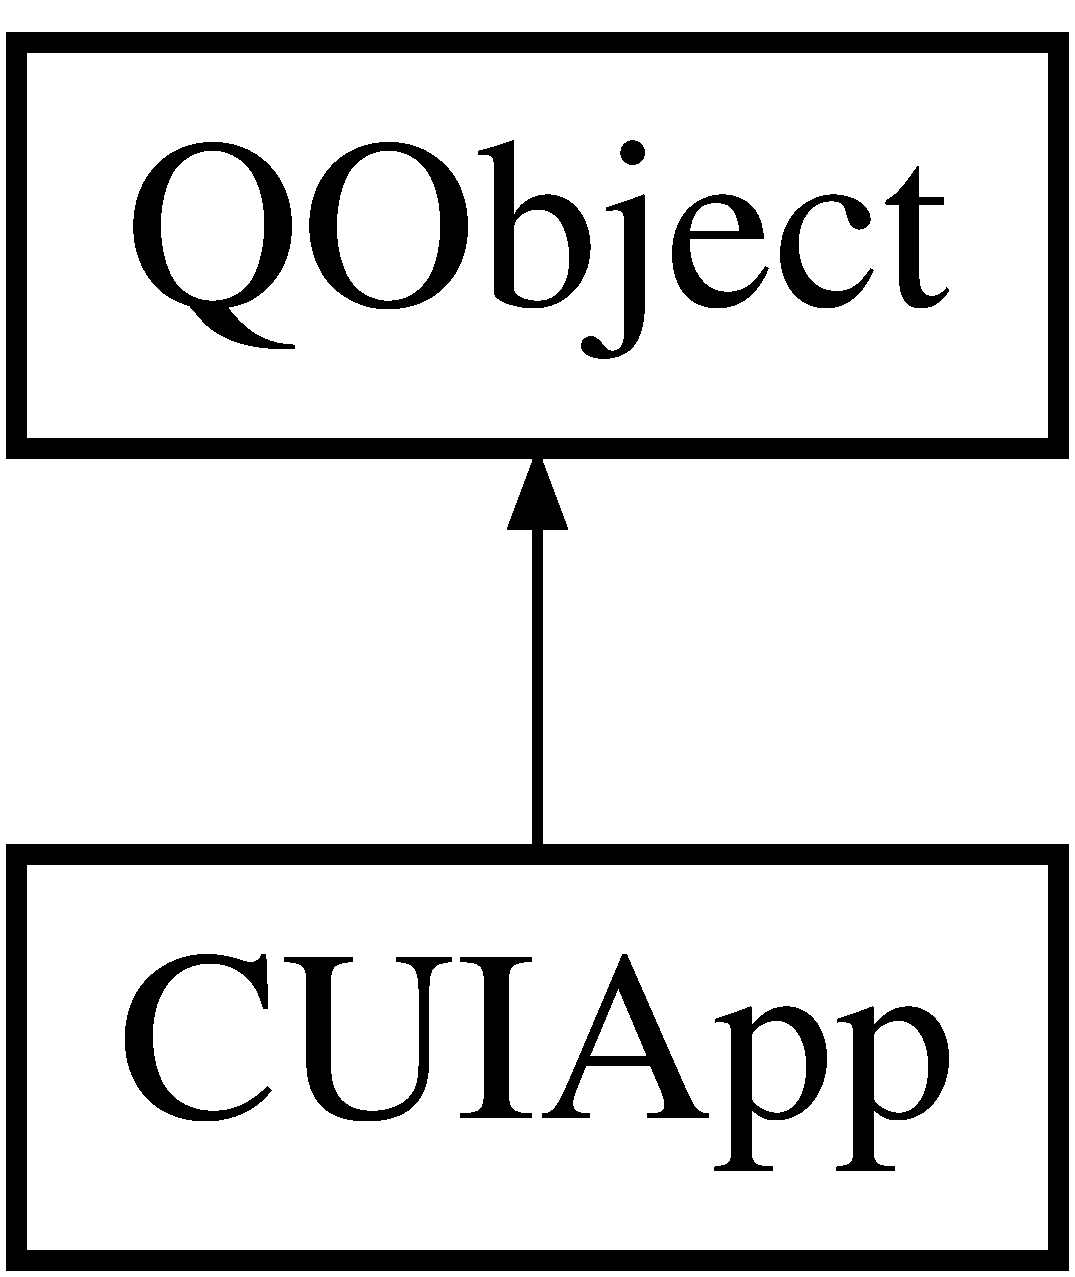
\includegraphics[height=2.000000cm]{classCUIApp}
\end{center}
\end{figure}
\subsection*{Signals}
\begin{DoxyCompactItemize}
\item 
void \hyperlink{classCUIApp_a9324e3388ce7ccfb3ec6b0862d61aa52}{receive\-Print\-Item} (const Q\-String \&str, int level)
\end{DoxyCompactItemize}
\subsection*{Public Member Functions}
\begin{DoxyCompactItemize}
\item 
\hyperlink{classCUIApp_afa0b05aa6039932ff99fda50db8e8110}{C\-U\-I\-App} (Q\-Object $\ast$parent=0)
\item 
void \hyperlink{classCUIApp_afd4cae5d66f7323cf38b9f1aed25f900}{set\-Standard\-Mode} (bool bstandard)
\item 
bool \hyperlink{classCUIApp_a0cc9cca9857c0bc9ef25230edc531ccf}{is\-Motor\-On} ()
\item 
bool \hyperlink{classCUIApp_ac8cab0d33456272cfe83542cba03788b}{is\-Motor\-On\-Switch} ()
\item 
bool \hyperlink{classCUIApp_a8e2b967299871e3f1c3a71e30d396f17}{is\-T\-P\-Enable} ()
\item 
bool \hyperlink{classCUIApp_a23dc5321e74f32f21bd32cbf8f483a42}{is\-Moving} ()
\item 
bool \hyperlink{classCUIApp_ac2c793ecc97fd8fdc13873bd425748c1}{is\-T\-P\-Inching} ()
\item 
bool \hyperlink{classCUIApp_a9b5b40e734cd6df6da5e5cb6b8d0f47b}{is\-Error} ()
\item 
bool \hyperlink{classCUIApp_abe557a84d4f46371691d64195f9bfdc1}{is\-Warning} ()
\item 
bool \hyperlink{classCUIApp_afede9804c9ff808fe7fda9cace46317a}{is\-Teach} ()
\item 
C\-N\-R\-\_\-\-T\-A\-S\-K\-\_\-\-S\-T\-A\-T\-U\-S \hyperlink{classCUIApp_a38b78efb82df844035218bf55d242446}{get\-Task\-Status} (int taskid)
\item 
bool \hyperlink{classCUIApp_a1cbbff02bbc244311de643be07f2ab50}{get\-Hold\-Done\-Status} ()
\item 
bool \hyperlink{classCUIApp_af1543e05abe6e4f10612a812f72ac2e4}{get\-Servo\-On} ()
\item 
int \hyperlink{classCUIApp_aa1f8e42c318759f87de95791a272e26d}{get\-Servo\-On2} ()
\item 
void \hyperlink{classCUIApp_a43c0f679870ab278c036ab542cfefe55}{set\-Servo\-On} (bool onoff)
\item 
bool \hyperlink{classCUIApp_a7b6b23d1380f0980aa23e54c588b50ef}{get\-Enabled} ()
\item 
void \hyperlink{classCUIApp_a0bb9aaecc950f991d3ecc69e5895e9e6}{set\-Enabled} (bool onoff)
\item 
bool \hyperlink{classCUIApp_a0e1919fc8bffe64510862903d2997746}{get\-Inching\-On} ()
\item 
void \hyperlink{classCUIApp_a875b8e4442379f90ce94c841bfb275ee}{set\-Inching\-On} (bool onoff)
\item 
int \hyperlink{classCUIApp_aed3628c3a5b2a214d95b66c158261469}{get\-Teach\-Speed} ()
\item 
void \hyperlink{classCUIApp_a48f2c72b1eedf48487c308c565102b04}{set\-Teach\-Speed} (int speed)
\item 
int \hyperlink{classCUIApp_a5a1b0c3f5b9ba0160e7fd04ce9045ad5}{get\-Jog\-Speed} (int level, float \&ratio)
\item 
int \hyperlink{classCUIApp_a7df9ad69084f03b2e610d0bc35769320}{set\-Jog\-Speed} (int level, float ratio)
\item 
int \hyperlink{classCUIApp_aa4adccaece246aa22b93d16219755521}{get\-Coordinate} ()
\item 
\hypertarget{classCUIApp_a20ea8f0c390d9ef552a006f153f4fbdf}{void {\bfseries set\-Coordinate} (int co)}\label{classCUIApp_a20ea8f0c390d9ef552a006f153f4fbdf}

\item 
int \hyperlink{classCUIApp_afae22d445cdef37f9c797084f16fc055}{get\-Use\-User\-Coord\-Flag} (bool $\ast$flag)
\item 
bool \hyperlink{classCUIApp_a51873975bdae2a082cf93ecd28592517}{get\-Hold\-Run} ()
\item 
void \hyperlink{classCUIApp_af3be79ba4b9c4feda7db65ea1c664d07}{set\-Hold\-Run} (bool b\-Hold)
\item 
bool \hyperlink{classCUIApp_a1e13081fe2b308c0ed6b48515d8e3ee1}{get\-Teach\-Mode} ()
\item 
void \hyperlink{classCUIApp_ac2f4c21479ef20f75ac6f5076835b15f}{set\-Teach\-Mode} (bool b\-Teach)
\item 
bool \hyperlink{classCUIApp_adaf17858538066ca486e6dba3cfe40bf}{get\-Check\-Mode} ()
\item 
int \hyperlink{classCUIApp_ab417f07d00c8d7804ee29dc16c9d1cef}{set\-Check\-Mode} (bool b\-Check\-Mode)
\item 
int \hyperlink{classCUIApp_a4806d708e39f2aa3392cdcfefe31fd28}{set\-Check\-Program} (const Q\-String \&prg\-Name, int index)
\item 
void \hyperlink{classCUIApp_af1cb9ef08858fc07b9fdb1a541c4f1a7}{set\-Check\-Key} (int check\-Key)
\item 
void \hyperlink{classCUIApp_a8810e1c9c6852373f02dd63c46b40aa9}{set\-Jog\-On} (unsigned int plus\-Key, unsigned int minus\-Key)
\item 
void \hyperlink{classCUIApp_a307e341b403a08fa1bb43738eff18698}{set\-Jog\-Off} (unsigned int plus\-Key, unsigned int minus\-Key)
\item 
int \hyperlink{classCUIApp_ab89ed3cfa8984f02170f51f064ef800b}{get\-Error\-Msg} (Q\-String \&error\-Msg)
\item 
int \hyperlink{classCUIApp_aa9b6b12846d38b038afdebb423e66d30}{get\-Last\-Error\-Info} (int \&error\-Code, int \&axis, int \&sub\-Code)
\item 
int \hyperlink{classCUIApp_a843c50491f63fba830c9d321b4af811b}{get\-Save\-Error\-List\-Size} ()
\item 
void \hyperlink{classCUIApp_abf330221079f242d37032e212d0cf401}{get\-Save\-Error\-List} (int errlist\mbox{[}$\,$\mbox{]}, int $\ast$nlist)
\item 
void \hyperlink{classCUIApp_a7e636d2d36cc25795e286cdc9b20b292}{reset\-Error} ()
\item 
void \hyperlink{classCUIApp_a49cb79bd21645b2247a7246c23178940}{reset\-Ecat\-Error} ()
\item 
void \hyperlink{classCUIApp_a4d7b7d79f9058f4788436b618c5d3f8c}{reset\-All\-Error} (bool bgmode=true)
\item 
bool \hyperlink{classCUIApp_a71f52cfd98a3b974e6e5bb18792022fa}{get\-Reset\-Error\-Status} ()
\item 
int \hyperlink{classCUIApp_af62220023edaab281f7ad32df8c7149d}{get\-Warning\-Code} (int \&warning\-Code)
\item 
int \hyperlink{classCUIApp_a65fd5f0b44938f9fd50b7ffa95beb2f3}{clear\-Warning\-Code} ()
\item 
int \hyperlink{classCUIApp_abb8769af70015d3d55aa180df9783c9b}{get\-E\-C\-A\-T\-Master\-Status} (int $\ast$status, int $\ast$nresponding, int $\ast$linkstatus)
\item 
int \hyperlink{classCUIApp_a80553db100390f6a3cba662ba79f0011}{get\-E\-C\-A\-T\-Domain\-Status} (int $\ast$wc, int $\ast$wc\-\_\-state)
\item 
void \hyperlink{classCUIApp_a16723ff044ecfcc4eac46f1190490261}{set\-E\-M\-G\-On} (bool on\-Off)
\item 
bool \hyperlink{classCUIApp_a37ba11617d17bd7876e678ad1a23080f}{get\-E\-M\-G\-On} ()
\item 
void \hyperlink{classCUIApp_ab08c13cf86c8600d6355a4b82d0d44cc}{filter\-System\-Key} (bool \hyperlink{classCUIApp_a0bb9aaecc950f991d3ecc69e5895e9e6}{set\-Enabled}=false)
\item 
bool \hyperlink{classCUIApp_a3929465084f3838bdcb958fffb3d6ee3}{get\-System\-Key\-Flag} ()
\item 
float $\ast$ \hyperlink{classCUIApp_a3044e8082b57b131955349a9e59d1341}{get\-Cur\-Joint} ()
\item 
float $\ast$ \hyperlink{classCUIApp_ad51349f53d180797ac563eee94b14305}{get\-Cur\-U\-C} ()
\item 
float $\ast$ \hyperlink{classCUIApp_a3644d18cbd1ba30478da55a8c36d759e}{get\-Cur\-Trans} ()
\item 
float $\ast$ \hyperlink{classCUIApp_a1d7f8fbb63c50f39d49a7b74b8df41e6}{get\-Cur\-V\-A\-Position} ()
\item 
float $\ast$ \hyperlink{classCUIApp_a6b09f14f5945d44728c84e4717a95aa6}{get\-Physical\-Joint} ()
\item 
int \hyperlink{classCUIApp_a01e8913a5caef79b31a1ca5f5473d406}{get\-Axis\-Count} ()
\item 
int \hyperlink{classCUIApp_add27a97e06315b685aabb293b4e9652f}{get\-D\-I} (cn\-\_\-ui32 $\ast$vals, int lenth)
\item 
int \hyperlink{classCUIApp_aa663db4584639c16d6fad80199d7b548}{set\-D\-I} (int vals)
\item 
int \hyperlink{classCUIApp_ade6a8c4817b025076a76d5d1c36c8f7a}{get\-D\-O} (cn\-\_\-ui32 $\ast$vals, int lenth)
\item 
int \hyperlink{classCUIApp_a994ecfe4ec23e565c0a7be4100867aa8}{set\-D\-O} (int $\ast$vals, int length)
\item 
int \hyperlink{classCUIApp_a15a6be8b534004d69462e879ca47d2cf}{get\-A\-I} (cn\-\_\-f32 $\ast$vals, int length)
\item 
int \hyperlink{classCUIApp_ab1953f84d2678e22425bdf2a77d721b7}{get\-A\-O} (cn\-\_\-f32 $\ast$vals, int length)
\item 
int \hyperlink{classCUIApp_aec709af257dd9baac1a891f3495902a3}{set\-A\-O} (int channel, cn\-\_\-f32 value)
\item 
int \hyperlink{classCUIApp_adef4e805121b59f9457b4ddf16aecbf8}{get\-Override\-D\-I\-N} (bool \&boverride)
\item 
int \hyperlink{classCUIApp_a1145d1a8d1db9391696cccecdee904d0}{set\-Override\-D\-I\-N} (bool boverride)
\item 
int \hyperlink{classCUIApp_ac5c2c5f0cebb36c358dc938a6eaaef6a}{get\-Programs} (Q\-String\-List \&pgms)
\item 
Q\-String \hyperlink{classCUIApp_a369cfe1db4b1f3d93e8f39ce9e3160e6}{get\-Cur\-Program\-Name} (int taskid, bool plan\-Program=false)
\item 
int \hyperlink{classCUIApp_a0b0973b55c62a2108e2f3a4b6e3d83f5}{set\-Cur\-Program} (int taskid, const Q\-String \&prg\-Name, int cycle=-\/1)
\item 
int \hyperlink{classCUIApp_ac137f1bd9ac1ada393c069943af1404c}{set\-Cur\-Step} (int taskid, int istrp)
\item 
int \hyperlink{classCUIApp_a15aeca2eb05975a0d22fdd92e3580f7a}{create\-Program} (const Q\-String \&prg\-Name)
\item 
int \hyperlink{classCUIApp_a12802aa0fbd6f6ec3ab9ef8a68ae3d5f}{delete\-Program} (const Q\-String \&prg\-Name)
\item 
int \hyperlink{classCUIApp_af7aa5b3cb8ec0e3053f2c594c2d53d33}{get\-Program\-Steps\-Count} (const Q\-String \&prg\-Name, int $\ast$step\-Count)
\item 
int \hyperlink{classCUIApp_acf883a14e463b52807f8eb1451db1e78}{get\-Cur\-Program\-Cycle} (int taskid)
\item 
int \hyperlink{classCUIApp_ad12e56e44ce01e82bd70616c0448598a}{get\-Program\-Run\-Count} (int taskid)
\item 
int \hyperlink{classCUIApp_ac9d5e6115e0369c90d96a58e208fe9ba}{set\-Program\-Run\-Count} (int taskid, int count)
\item 
bool \hyperlink{classCUIApp_a9fdc1f0419dbfb6fb9b5c699443aaa6f}{find\-Program} (const Q\-String \&prg\-Name)
\item 
int \hyperlink{classCUIApp_ac6aae50ce175ebb747b3cf6a09eac470}{get\-Programs\-Count} ()
\item 
int \hyperlink{classCUIApp_abb18a18a93e84838a34d99e10aa0b036}{insert\-Step} (const Q\-String \&prg\-Name, const Q\-String \&step\-Name, int index=1)
\item 
int \hyperlink{classCUIApp_a228f715f0ab12f6903fe78d4ce5fac8d}{delete\-Step} (const Q\-String \&prg\-Name, int index)
\item 
int \hyperlink{classCUIApp_a8829edc5cbe151eb81e310080f95e6b9}{get\-Program\-Steps} (const Q\-String \&prg\-Name, Q\-String\-List \&steps)
\item 
int \hyperlink{classCUIApp_a7cada6fdcbaf4f3390726ba03bb5f164}{set\-Program\-Steps} (const Q\-String \&prg\-Name, Q\-String\-List \&steps)
\item 
int \hyperlink{classCUIApp_a037de6d8be99831562b1c157eef1cfae}{save\-Program} (const Q\-String \&prg\-Name)
\item 
int \hyperlink{classCUIApp_a762c36f582d0f2d80280129a5cfa8845}{save\-Program\-All} ()
\item 
int \hyperlink{classCUIApp_a82d14569d3fb78a02379cd061233754c}{execute\-Command} (char $\ast$str)
\item 
int \hyperlink{classCUIApp_a3725056976dca5ff4421b818e19aba41}{execute\-Program} (int taskid, const Q\-String \&prg\-Name, int cycle)
\item 
int \hyperlink{classCUIApp_a800f6928aa302c9898282b33d6f67063}{hold\-Program} (int taskid)
\item 
int \hyperlink{classCUIApp_acbf70cc0ff1d7a7d470424065984c37d}{abort\-Program} (int taskid)
\item 
int \hyperlink{classCUIApp_ac9e8075a0d1645830b451870368be7d7}{continue\-Program} (int taskid)
\item 
int \hyperlink{classCUIApp_a1418345bd5ea072ad265e1832da5be1c}{clear\-Cur\-Program} (int taskid)
\item 
int \hyperlink{classCUIApp_aab24a02fe45512a2d04a03cf308f4846}{reset\-Cur\-Program} (int taskid)
\item 
int \hyperlink{classCUIApp_a1cb0b7f420d5c736eabe5aeade669684}{run\-Nxt\-Step} (int taskid)
\item 
int \hyperlink{classCUIApp_a259d5dab2d54a11caf34c15cf8b7d7cc}{run\-Nxt\-Step\-Over} (int taskid)
\item 
int \hyperlink{classCUIApp_acf6132d19e753ba5548f9af6fbcaaa32}{run\-To\-Next\-Motion\-Step} ()
\item 
int \hyperlink{classCUIApp_a53d60c9f8804ed89187d1d06b0afb14c}{run\-Back\-Step} (int taskid)
\item 
int \hyperlink{classCUIApp_aa7570a64d24746ae8e876b78bafef329}{run\-Back\-Step\-Over} (int taskid)
\item 
int \hyperlink{classCUIApp_a44cdd21e80259e4718a443737e881cc1}{move\-To\-Position} (const Q\-String \&var\-Name, bool is\-Linear=false)
\item 
int \hyperlink{classCUIApp_ae6fb6a202f9d1a189c093eeb5e4ad4a9}{move\-To\-Position2} (const Q\-String \&var\-Name, float stable\-Time=0.f, bool is\-Linear=false)
\item 
int \hyperlink{classCUIApp_ab9ad5f3f98559557dcac912771043d34}{set\-Stable\-Time} (float time)
\item 
int \hyperlink{classCUIApp_ab37f3a8b7d7e183c81ba807b2e808cd8}{get\-Running\-Step\-Index} (int taskid, int $\ast$movestep, int $\ast$planstep)
\item 
int \hyperlink{classCUIApp_af00947fd23c355c47bfc4601ba4db337}{get\-Running\-Main\-Step\-Index} (int $\ast$planstep, int taskid=0)
\item 
int \hyperlink{classCUIApp_a5260cf4599017e2da6c99295dd6b9558}{set\-Speed} (float speed)
\item 
int \hyperlink{classCUIApp_a916a3ae9eea10c497d29b1ffc0a0af1a}{get\-Override\-Speed} ()
\item 
int \hyperlink{classCUIApp_a40a04b9026dff73dac5f426700205fdc}{get\-Cur\-Program\-Stack} (int taskid, Q\-String\-List \&str\-List)
\item 
int \hyperlink{classCUIApp_af3f0a39e3dacc4ab67611e527f91a53a}{get\-Auto\-Run\-Sub\-Program} (bool \&\hyperlink{classCUIApp_a0bb9aaecc950f991d3ecc69e5895e9e6}{set\-Enabled}, int taskid=1)
\item 
int \hyperlink{classCUIApp_a7ec5fc0b595cc0744216a3ea157db1e3}{set\-Auto\-Run\-Sub\-Program} (bool \hyperlink{classCUIApp_a0bb9aaecc950f991d3ecc69e5895e9e6}{set\-Enabled}, int taskid=1)
\item 
int \hyperlink{classCUIApp_af7fb38556ebd9cb1dab1c054170f9918}{get\-Variable\-Count} (int type, int $\ast$count)
\item 
int \hyperlink{classCUIApp_ae70f81bcbc00de588c4c50d1b556da10}{get\-Variable\-Name} (int type, int index, Q\-String \&varname)
\item 
int \hyperlink{classCUIApp_a925db4d1b2bbd1afb9444c0e0107e8b0}{get\-Variable\-List\-All} (int type, Q\-String\-List \&varname, Q\-Vector$<$ \hyperlink{structcn__variant}{cn\-\_\-variant} $>$ \&vardata\-List)
\item 
int \hyperlink{classCUIApp_aa91bb1b3ee8cd64c045070501febc093}{get\-Variable\-List} (int type, Q\-String\-List \&varname, Q\-Vector$<$ \hyperlink{structcn__variant}{cn\-\_\-variant} $>$ \&vardata\-List)
\item 
int \hyperlink{classCUIApp_a2e1f43703c1671c83597eb4c49fcdb84}{get\-Variable\-Data} (int type, const Q\-String \&varname, \hyperlink{structcn__variant}{cn\-\_\-variant} $\ast$value)
\item 
int \hyperlink{classCUIApp_a1278c6736ec4e320ded37fcf47c7f947}{set\-Variable\-Data} (int type, const Q\-String \&varname, \hyperlink{structcn__variant}{cn\-\_\-variant} \&value, bool create\-Non\-Exist)
\item 
int \hyperlink{classCUIApp_ab3516417e2cea5be658322391350312e}{delete\-Variable} (int type, const Q\-String \&varname)
\item 
int \hyperlink{classCUIApp_ad515e95f6925fb50d6945baee291b017}{delete\-Variable\-All} ()
\item 
int \hyperlink{classCUIApp_aa79bafb099375e6dd3abc597282a5637}{get\-Variable\-Type} (const Q\-String \&varname, int \&type, int \&dimension, int \&exist)
\item 
int \hyperlink{classCUIApp_af85b9d32033d3eb9fccf453d074e3be8}{get\-Variables} (Q\-String\-List \&varnames, Q\-List$<$ \hyperlink{structcn__variant}{cn\-\_\-variant} $>$ \&values)
\item 
int \hyperlink{classCUIApp_aa8642ecf51f34f93073e5708586ad56c}{set\-Variables} (Q\-String\-List \&varnames, Q\-List$<$ \hyperlink{structcn__variant}{cn\-\_\-variant} $>$ \&values)
\item 
void \hyperlink{classCUIApp_ad06f7d4fe267316a5f408b20b380fc3e}{save\-Variable} ()
\item 
int \hyperlink{classCUIApp_ac406cc3f26f1b415e145cd0bee60b46e}{get\-Variable\-Auto\-Save} (bool \&\hyperlink{classCUIApp_a0bb9aaecc950f991d3ecc69e5895e9e6}{set\-Enabled})
\item 
int \hyperlink{classCUIApp_a3c0ac9e02ec745c05658c8ab58b8bc02}{set\-Variable\-Auto\-Save} (bool \hyperlink{classCUIApp_a0bb9aaecc950f991d3ecc69e5895e9e6}{set\-Enabled})
\item 
int \hyperlink{classCUIApp_a64d3d2e86624b51e5f990ac73b85f9ec}{zeroing} (unsigned long axis\-\_\-mask)
\item 
int \hyperlink{classCUIApp_aaf099c230d05b323f5ab62c25ca040ba}{zeroing\-Count} (long $\ast$penc)
\item 
int \hyperlink{classCUIApp_a2936477854549f24236662a1967c0c78}{set\-Zeroing\-Offset} (float $\ast$pos\-Array, int naxis)
\item 
int \hyperlink{classCUIApp_ade2fe0edbcadb0d9c31e23db494033c3}{get\-Zeroing\-Offset} (float $\ast$pos\-Array)
\item 
int \hyperlink{classCUIApp_a02a5f7d94a6ca9ba0c050574e8fb9ee5}{get\-Log\-List} (Q\-String\-List \&loglist)
\item 
int \hyperlink{classCUIApp_abbe30c42f3161debd9c5b61c4afea678}{set\-User\-Log} (int code, const Q\-String \&msg)
\item 
void \hyperlink{classCUIApp_a803e0e51595b7d38ead94d1fe6cae849}{clear\-Log\-Mask} ()
\item 
int \hyperlink{classCUIApp_a29dc28296cfb8e9271cd0b77fa13789a}{add\-Log\-Mask} (int from, int to)
\item 
int \hyperlink{classCUIApp_a2590acef111dbbaa876de86ac1b323a5}{get\-Log\-Mask\-Size} (int \&size)
\item 
int \hyperlink{classCUIApp_ad4f668fddc3ba074f8006bc13b6fa445}{get\-Log\-Mask} (int index, int \&from, int \&to)
\item 
int \hyperlink{classCUIApp_a174d987f2079552ee55978771061dc9b}{enque\-Print\-List\-Item} (int level, const Q\-String \&msg)
\item 
int \hyperlink{classCUIApp_a997e16c024559902626cc6fc98c9ef6b}{get\-I\-O\-Count} (C\-N\-R\-\_\-\-S\-L\-A\-V\-E\-\_\-\-T\-Y\-P\-E type, int \&Count)
\item 
int \hyperlink{classCUIApp_a36a0dd9664cf48673640716277638e58}{get\-Slave\-Count} (int \&count)
\item 
int \hyperlink{classCUIApp_ada4c7ae52850321862eb34f6c3190af6}{get\-Slave\-Type} (Q\-Vector$<$ C\-N\-R\-\_\-\-S\-L\-A\-V\-E\-\_\-\-T\-Y\-P\-E $>$ \&v\-Slv\-Type)
\item 
int \hyperlink{classCUIApp_aef270c9f46a09ee42c4a6213e6a0ef3f}{get\-Slave\-Model} (Q\-String\-List \&slv\-List)
\item 
int \hyperlink{classCUIApp_a3f28630e81a274fb998aec04e17992f2}{set\-Enable\-Deivated\-Signal} (C\-N\-R\-\_\-\-D\-D\-C\-\_\-\-S\-I\-G\-N\-A\-L signal, bool \hyperlink{classCUIApp_a0bb9aaecc950f991d3ecc69e5895e9e6}{set\-Enabled})
\item 
int $\ast$ \hyperlink{classCUIApp_a4a20047ab2d7ec753785db2b4b955666}{get\-Motor\-Actual\-Velocity} ()
\item 
int $\ast$ \hyperlink{classCUIApp_a022c1b824525745e09c6080c22ac179a}{get\-Motor\-Actual\-Torque} ()
\item 
long $\ast$ \hyperlink{classCUIApp_a3c11238c75f11140c7bc79ec6c69d175}{get\-P\-D\-O\-T\-\_\-\-Following\-Error} ()
\item 
long $\ast$ \hyperlink{classCUIApp_a7b5fcf976a2f6b7c5d396ad379cfe30a}{get\-P\-D\-O\-T\-\_\-\-Velocity} ()
\item 
short $\ast$ \hyperlink{classCUIApp_a1aad67b6ffa78081b285c4b55b601b93}{get\-P\-D\-O\-T\-\_\-\-Torque} ()
\item 
int $\ast$ \hyperlink{classCUIApp_adfc9ee94df8b0e299985f4e7de4e9755}{get\-P\-D\-O\-T\-\_\-\-Status\-Word} ()
\item 
int \hyperlink{classCUIApp_a339bd304f36c7eafa52efd7d06742b33}{get\-S\-D\-O} (int id, int $\ast$args, int lenth, unsigned long $\ast$data\-List)
\item 
int \hyperlink{classCUIApp_a7db69eefe8a46e4e7b2791ada7efe719}{set\-S\-D\-O} (int id, int $\ast$args, int lenth, unsigned long $\ast$data\-List)
\item 
int \hyperlink{classCUIApp_af91843d583fe4bd9b12abf1ea1d04bea}{get\-S\-D\-O\-List} (int $\ast$args, int arg\-Lenth, unsigned long $\ast$data\-List, int \&data\-Lenth)
\item 
int \hyperlink{classCUIApp_ad6d72a0b565f779b61eb0b4e71810a77}{get\-T\-P\-Write} (Q\-String\-List \&str\-List, Q\-Vector$<$ C\-N\-R\-\_\-\-T\-P\-\_\-\-M\-S\-G\-\_\-\-S\-T\-A\-T\-U\-S $>$ \&msg\-Status)
\item 
int \hyperlink{classCUIApp_af65c69d76062c8c0b9eded1761c1e7e9}{get\-User\-Params} (Q\-String\-List \&params)
\item 
int \hyperlink{classCUIApp_a8e509954cca273e527eafc4fde64a0b2}{set\-User\-Params} (Q\-String\-List params)
\item 
int \hyperlink{classCUIApp_a674f263816eeb0bdb7b68439f421260a}{get\-Robot\-Conf} (Q\-String\-List \&data\-List)
\item 
int \hyperlink{classCUIApp_a72fc3d4ed526cc68125ad588f67b5425}{set\-Robot\-Conf} (Q\-String\-List data\-List)
\item 
int \hyperlink{classCUIApp_a9a5718d007c4d0dec21ad234a2827dc2}{get\-Robot\-Name} (Q\-String \&robot\-Name)
\item 
C\-N\-R\-\_\-\-M\-E\-C\-H\-\_\-\-T\-Y\-P\-E \hyperlink{classCUIApp_a33d884ef8a808b2868dbbc47e05e2ac2}{get\-Robot\-Type} ()
\item 
int \hyperlink{classCUIApp_a194fa60ec23503459897381d36f41706}{get\-Date\-Time} (Q\-String \&str\-Time)
\item 
int \hyperlink{classCUIApp_a62cfddfc18a235f0cfc6ea7e168f37ce}{set\-Date\-Time} (Q\-String str\-Time)
\item 
int \hyperlink{classCUIApp_a2ae1abae4dd4aaf40332b127c3fc5b13}{reboot\-System} ()
\item 
int \hyperlink{classCUIApp_a9b47dc610983417f16fcd26a78386814}{set\-D\-P\-T\-Buzzer\-On} (int count, int interval)
\item 
int \hyperlink{classCUIApp_a53a903ed784f511799d39a920d6c1618}{set\-D\-P\-T\-Buzzer\-Off} ()
\item 
int \hyperlink{classCUIApp_acb86ae6150571428671015ef6859826e}{set\-D\-T\-P\-Led} (C\-N\-R\-\_\-\-L\-E\-D led\-Pos, C\-N\-R\-\_\-\-L\-E\-D\-\_\-\-C\-O\-L\-O\-R led\-Color)
\item 
bool \hyperlink{classCUIApp_a779ad6bc661533b3c75a3f8f8cce2ece}{get\-Debug\-Flag} ()
\item 
int \hyperlink{classCUIApp_a1566cbcfdf9a3eb4f8c841edffa00dcc}{get\-Cur\-Base\-Name} (Q\-String \&base\-Name)
\item 
int \hyperlink{classCUIApp_a7536797eac45ecf5beb09f5fe2765b0a}{get\-Cur\-Tool\-Name} (Q\-String \&tool\-Name)
\item 
int \hyperlink{classCUIApp_a2b00b9e3246df2c98ab2303e3988049e}{get\-Inching\-Step} (int level, float \&step\-\_\-mm)
\item 
int \hyperlink{classCUIApp_a73b625566370601ba8a7c581b6426090}{set\-Inching\-Step} (int level, float step\-\_\-mm)
\item 
int \hyperlink{classCUIApp_ac424a7fd3fec4d813638342c80eefe64}{get\-Inching\-Step\-Angular} (int level, float \&step\-\_\-deg)
\item 
int \hyperlink{classCUIApp_a34d6c57d939b7b5750ace5b630f11114}{set\-Inching\-Step\-Angular} (int level, float step\-\_\-deg)
\item 
int \hyperlink{classCUIApp_a8f49d15e94fa3339041d11b121c0f81a}{get\-Inching\-Acc\-Time} (float \&acctime)
\item 
int \hyperlink{classCUIApp_a19bc933038b12820648d71d494719809}{set\-Inching\-Acc\-Time} (float acctime)
\item 
int \hyperlink{classCUIApp_aff9bfd02433068705595b74ed50b5d6e}{set\-Home\-Start} ()
\item 
int \hyperlink{classCUIApp_abcf462661e4d7a92b36a6a1bea7bc036}{set\-Home\-Stop} ()
\item 
C\-N\-R\-\_\-\-H\-O\-M\-E\-\_\-\-S\-T\-A\-T\-U\-S \hyperlink{classCUIApp_a2151edd77746c8862cc46f02319b0274}{get\-Home\-Status} ()
\item 
int \hyperlink{classCUIApp_a478a122cd1d492055b063a6836a33212}{get\-Home\-Position} (int index, float $\ast$pos, int npos, float \&bound)
\item 
int \hyperlink{classCUIApp_ab3595ed37eb43bb0c552623806e90249}{set\-Home\-Position} (int index, float $\ast$pos, int npos, float bound)
\item 
int \hyperlink{classCUIApp_ae4246ee91a5f098604d03d8459f1b634}{move\-To\-Home} (int index=0)
\item 
int \hyperlink{classCUIApp_a392d9f88563aa020c997f11a829dc909}{get\-Euler\-Angle\-Type} (C\-N\-R\-\_\-\-E\-U\-L\-E\-R\-\_\-\-A\-N\-G\-L\-E\-\_\-\-T\-Y\-P\-E \&type)
\item 
int \hyperlink{classCUIApp_a18eca8206aa0eedab39af17c3e55c511}{set\-Euler\-Angle\-Type} (C\-N\-R\-\_\-\-E\-U\-L\-E\-R\-\_\-\-A\-N\-G\-L\-E\-\_\-\-T\-Y\-P\-E type)
\item 
int \hyperlink{classCUIApp_aec69bd13266bc0bb999b2f3d28bc17b3}{get\-Hybrid\-Jog\-Mode} (bool \&hybrid, C\-N\-R\-\_\-\-H\-Y\-B\-\_\-\-J\-O\-G\-\_\-\-T\-Y\-P\-E xyzrpy\mbox{[}$\,$\mbox{]}, int ntype)
\item 
int \hyperlink{classCUIApp_a4d5e32f869d8cd37f595ac0581c548c0}{set\-Hybrid\-Jog\-Mode} (bool hybrid, C\-N\-R\-\_\-\-H\-Y\-B\-\_\-\-J\-O\-G\-\_\-\-T\-Y\-P\-E xyzrpy\mbox{[}$\,$\mbox{]}, int ntype)
\item 
int \hyperlink{classCUIApp_af643f6bcefda4737060fb9225a304ed8}{set\-Soft\-Limit\-Monitor\-Flag} (bool \hyperlink{classCUIApp_a0bb9aaecc950f991d3ecc69e5895e9e6}{set\-Enabled})
\item 
bool \hyperlink{classCUIApp_a87e000f4f97ea7f78c3e40cb2ed305cd}{get\-Soft\-Limit\-Monitor\-Flag} ()
\item 
unsigned char \hyperlink{classCUIApp_a339658f6d6002aa770b0a0a416653904}{get\-W\-Z\-Check\-Flag} ()
\item 
int \hyperlink{classCUIApp_a186fff0fa0564e376726df78bf31802f}{set\-W\-Z\-Check\-Flag} (unsigned char flag)
\item 
int \hyperlink{classCUIApp_ab5c2ed7bd5bacb715485e286e3d9e33e}{W\-Z\-Clear} (int index)
\item 
int \hyperlink{classCUIApp_a7ae08ed44f496fe5a3eeb0ec2c828fdb}{W\-Z\-Add\-Box} (int index, int op, \hyperlink{structcn__vec3}{cn\-\_\-vec3} \&pmin, \hyperlink{structcn__vec3}{cn\-\_\-vec3} \&pmax, \hyperlink{structcn__trans2}{cn\-\_\-trans2} \&frame)
\item 
int \hyperlink{classCUIApp_a499e134cf18fc918a83e0cd31fd56ba6}{W\-Z\-Add\-Cyl} (int index, int op, \hyperlink{structcn__vec3}{cn\-\_\-vec3} \&pc, float r, float h, \hyperlink{structcn__trans2}{cn\-\_\-trans2} \&frame)
\item 
int \hyperlink{classCUIApp_a9431ce97ebd52d159463c139c9dae083}{W\-Z\-Enable} (int index, int is\-\_\-negate)
\item 
int \hyperlink{classCUIApp_a2183043cadcc4afbebbd6afc10e57313}{W\-Z\-Disable} (int index)
\item 
int \hyperlink{classCUIApp_adc50b08e02682b5e3f1e002d31040e4c}{W\-Z\-Get\-Flag} (int index, int \&is\-\_\-enabled, int \&is\-\_\-negate)
\item 
int \hyperlink{classCUIApp_addb92c34a41a38e8688ec8c16da6396a}{W\-Z\-Get\-Entity\-Count} (int index, int \&count)
\item 
int \hyperlink{classCUIApp_aeb65cce62258e48239d713554e062794}{W\-Z\-Get\-Entity\-Type} (int index, int entity\-\_\-index, int \&type)
\item 
int \hyperlink{classCUIApp_a716eda397e3bec88da602c18b0e91556}{W\-Z\-Get\-Entity\-Box} (int index, int entity\-\_\-index, \hyperlink{structcn__vec3}{cn\-\_\-vec3} \&pmin, \hyperlink{structcn__vec3}{cn\-\_\-vec3} \&pmax)
\item 
int \hyperlink{classCUIApp_a72a74c0cbd2242374cf69b53a9c03e36}{W\-Z\-Get\-Entity\-Cyl} (int index, int entity\-\_\-index, \hyperlink{structcn__vec3}{cn\-\_\-vec3} \&pc, float \&radius, float \&height)
\item 
int \hyperlink{classCUIApp_a4e3483222d1296c96d04e46e28b03715}{W\-Z\-Get\-Entity\-Frame} (int index, int entity\-\_\-index, \hyperlink{structcn__trans2}{cn\-\_\-trans2} \&frame)
\item 
int \hyperlink{classCUIApp_ab90f33b53859cf92935b2e8b4618d747}{W\-Z\-Get\-Entity\-Operator} (int index, int entity\-\_\-index, int \&op)
\item 
int \hyperlink{classCUIApp_aacac360f0c6dd5a21ddc672a7ae8c52b}{W\-Z\-Save\-All} ()
\item 
int \hyperlink{classCUIApp_a2b36c2c000c8ac40267a32e5588874b9}{get\-Z\-Comp\-Table\-Size} (int tblidx, int \&size)
\item 
int \hyperlink{classCUIApp_a9c2d0d375c5ebfdd37bf8eb8c070248e}{clear\-Z\-Comp\-Table} (int tblidx)
\item 
int \hyperlink{classCUIApp_a4f1db639671b867b5d77821a2a9bbf59}{add\-Z\-Comp\-Table\-Item} (int tblidx, float r, float z)
\item 
int \hyperlink{classCUIApp_ab5aba87f4504310bacaa9472d86749f6}{get\-Z\-Comp\-Table\-Item} (int tblidx, int index, float \&r, float \&z)
\item 
int \hyperlink{classCUIApp_a421e0358fe93ca66e0f7a74f6c4075b2}{set\-Z\-Comp\-Table\-Item} (int tblidx, int index, float r, float z)
\item 
int \hyperlink{classCUIApp_a8c27562518b7b419056798edfcd2581c}{clac\-Inverse} (\hyperlink{structcn__trans}{cn\-\_\-trans} \&tr\-In, float $\ast$oldang, float $\ast$jnt\-Out, \hyperlink{structcn__conf}{cn\-\_\-conf} \&conf\-In)
\item 
bool \hyperlink{classCUIApp_a5e01da316ce0b59ae5780ef55c1fb9af}{get\-Repeat\-Cycle\-Sync\-Motion\-Flag} ()
\item 
int \hyperlink{classCUIApp_a677a189567521410686a0f302fcb88a2}{set\-Repeat\-Cycle\-Sync\-Motion\-Flag} (bool flag)
\item 
int \hyperlink{classCUIApp_a00d24384842a8f89965038629122628d}{set\-Run\-Sequence\-Timer} (float servo\-\_\-on, float brake\-\_\-on, float run\-\_\-ok)
\item 
int \hyperlink{classCUIApp_a66980bb62ac3fee3ce2eda42cdf632b9}{get\-Run\-Sequence\-Timer} (float \&servo\-\_\-on, float \&brake\-\_\-on, float \&run\-\_\-ok)
\item 
\hypertarget{classCUIApp_aa7d6a48216718947d460c53ef50e20d3}{void {\bfseries raise\-Receive\-Print\-Item\-Signal} (const Q\-String \&str, int level)}\label{classCUIApp_aa7d6a48216718947d460c53ef50e20d3}

\item 
int \hyperlink{classCUIApp_a9d18970cff5ce1265a65098c5a866dcb}{show\-Number\-Dialog} (const Q\-String \&str\-In, Q\-String \&str\-Out)
\item 
int \hyperlink{classCUIApp_a8cec29d70ac25427f29b774ba441202c}{show\-Password\-Dialog} (const Q\-String \&str\-In, Q\-String \&str\-Out)
\item 
int \hyperlink{classCUIApp_a8601870e0a38673fb01b2c4434370f5b}{show\-Hex\-Dialog} (const Q\-String \&str\-In, Q\-String \&str\-Out)
\item 
int \hyperlink{classCUIApp_a88513c30feec1d4fe8066371ca112d71}{show\-Keyboard\-Dialog} (Q\-String \&str)
\item 
int \hyperlink{classCUIApp_ae2633f43e94dfb880ff1277699226519}{show\-Home\-Search\-Dialog} ()
\item 
int \hyperlink{classCUIApp_aaa47294e1b6c6c671c5c0bdd94091a83}{show\-Set\-Inching\-Dialog} ()
\item 
int \hyperlink{classCUIApp_a13a1b4f0cc4b06e300cec033532735b7}{show\-Program\-List\-Dialog} (const Q\-String \&str\-In, Q\-String \&str\-Out)
\item 
bool \hyperlink{classCUIApp_af86f04f24e5529f99e952d69b9a9c787}{get\-Dry\-Run\-Mode} ()
\item 
int \hyperlink{classCUIApp_aa3d417803b6914e8b5b9d7ddb58d4efd}{get\-Min\-Torque\-Log\-Data} (int axis, short \&log\-Data)
\item 
int \hyperlink{classCUIApp_a43b0348d921203b6d15874b3f56a8298}{get\-Max\-Torque\-Log\-Data} (int axis, short \&log\-Data)
\item 
int \hyperlink{classCUIApp_a5c062b76fb34f6585138cecfddecaebf}{get\-Average\-Torque\-Log\-Data} (int axis, short \&log\-Data)
\item 
int \hyperlink{classCUIApp_a13fb4cbbb6da8eaddd3559291346a17d}{start\-Torque\-Data\-Logging} (bool flag)
\item 
int \hyperlink{classCUIApp_a316cae00cda86a676ec0dc350b0f985e}{set\-Torque\-Limit\-Monitor\-Flag} (bool flag)
\item 
int \hyperlink{classCUIApp_a2817d696dbe549b3e5024b5710c36aaa}{set\-Torque\-Limit\-Value} (int axis, short positive, short negative)
\item 
int \hyperlink{classCUIApp_afec821ab1d2fbe6c56f3824e9eca0452}{set\-Kalman\-Filter\-Volumn} (int volumn)
\item 
int \hyperlink{classCUIApp_a4c947f133769866ed8f83ca0fb26b8bf}{reset\-Min\-Max\-Torque\-Data} ()
\item 
int \hyperlink{classCUIApp_a50b55afe3b66bc00cb1e2e34ed8db2b0}{get\-Version} (C\-N\-R\-\_\-\-V\-E\-R\-S\-I\-O\-N\-\_\-\-T\-Y\-P\-E type, Q\-String \&version)
\end{DoxyCompactItemize}
\subsection*{Static Public Member Functions}
\begin{DoxyCompactItemize}
\item 
\hypertarget{classCUIApp_a22bded8c962f876f02b38f6cdc1fbfa2}{static \hyperlink{classCUIApp}{C\-U\-I\-App} $\ast$ {\bfseries get\-Instance} ()}\label{classCUIApp_a22bded8c962f876f02b38f6cdc1fbfa2}

\end{DoxyCompactItemize}


\subsection{Constructor \& Destructor Documentation}
\hypertarget{classCUIApp_afa0b05aa6039932ff99fda50db8e8110}{\index{C\-U\-I\-App@{C\-U\-I\-App}!C\-U\-I\-App@{C\-U\-I\-App}}
\index{C\-U\-I\-App@{C\-U\-I\-App}!CUIApp@{C\-U\-I\-App}}
\subsubsection[{C\-U\-I\-App}]{\setlength{\rightskip}{0pt plus 5cm}C\-U\-I\-App\-::\-C\-U\-I\-App (
\begin{DoxyParamCaption}
\item[{Q\-Object $\ast$}]{parent = {\ttfamily 0}}
\end{DoxyParamCaption}
)\hspace{0.3cm}{\ttfamily [explicit]}}}\label{classCUIApp_afa0b05aa6039932ff99fda50db8e8110}

\begin{DoxyParams}{Parameters}
{\em parent} & \\
\hline
\end{DoxyParams}


\subsection{Member Function Documentation}
\hypertarget{classCUIApp_acbf70cc0ff1d7a7d470424065984c37d}{\index{C\-U\-I\-App@{C\-U\-I\-App}!abort\-Program@{abort\-Program}}
\index{abort\-Program@{abort\-Program}!CUIApp@{C\-U\-I\-App}}
\subsubsection[{abort\-Program}]{\setlength{\rightskip}{0pt plus 5cm}int C\-U\-I\-App\-::abort\-Program (
\begin{DoxyParamCaption}
\item[{int}]{taskid}
\end{DoxyParamCaption}
)}}\label{classCUIApp_acbf70cc0ff1d7a7d470424065984c37d}
Abort the working macro \par
 if set the abort command, macro will be stop after the current step finish. 
\begin{DoxyParams}[1]{Parameters}
\mbox{\tt in}  & {\em taskid} & 0, 100 $\sim$ 109 \-: main task 1, 110 $\sim$ 119 \-: sub task \\
\hline
\end{DoxyParams}
\begin{DoxyReturn}{Returns}
success 0 
\end{DoxyReturn}
\hypertarget{classCUIApp_a29dc28296cfb8e9271cd0b77fa13789a}{\index{C\-U\-I\-App@{C\-U\-I\-App}!add\-Log\-Mask@{add\-Log\-Mask}}
\index{add\-Log\-Mask@{add\-Log\-Mask}!CUIApp@{C\-U\-I\-App}}
\subsubsection[{add\-Log\-Mask}]{\setlength{\rightskip}{0pt plus 5cm}int C\-U\-I\-App\-::add\-Log\-Mask (
\begin{DoxyParamCaption}
\item[{int}]{from, }
\item[{int}]{to}
\end{DoxyParamCaption}
)}}\label{classCUIApp_a29dc28296cfb8e9271cd0b77fa13789a}
Masking the log code 
\begin{DoxyParams}[1]{Parameters}
\mbox{\tt in}  & {\em from} & Start log code number \\
\hline
\mbox{\tt in}  & {\em to} & Eng log code number \\
\hline
\end{DoxyParams}
\begin{DoxyReturn}{Returns}
success 0 
\end{DoxyReturn}
\hypertarget{classCUIApp_a4f1db639671b867b5d77821a2a9bbf59}{\index{C\-U\-I\-App@{C\-U\-I\-App}!add\-Z\-Comp\-Table\-Item@{add\-Z\-Comp\-Table\-Item}}
\index{add\-Z\-Comp\-Table\-Item@{add\-Z\-Comp\-Table\-Item}!CUIApp@{C\-U\-I\-App}}
\subsubsection[{add\-Z\-Comp\-Table\-Item}]{\setlength{\rightskip}{0pt plus 5cm}int C\-U\-I\-App\-::add\-Z\-Comp\-Table\-Item (
\begin{DoxyParamCaption}
\item[{int}]{tblidx, }
\item[{float}]{r, }
\item[{float}]{z}
\end{DoxyParamCaption}
)}}\label{classCUIApp_a4f1db639671b867b5d77821a2a9bbf59}
Add z-\/compensation data in the selected index. z-\/compensation \-: Compensate the deflection due to gravity, 
\begin{DoxyParams}[1]{Parameters}
\mbox{\tt in}  & {\em tblidx} & zcomp table index \\
\hline
\mbox{\tt in}  & {\em r} & X\-Y plane distance between T\-C\-P position and zero position \\
\hline
\mbox{\tt in}  & {\em z} & z-\/axis compensate unit \-: mm Z-\/axis direction must be set oppesite from the deflection direction \\
\hline
\end{DoxyParams}
\begin{DoxyReturn}{Returns}
success 0 
\end{DoxyReturn}
\hypertarget{classCUIApp_a8c27562518b7b419056798edfcd2581c}{\index{C\-U\-I\-App@{C\-U\-I\-App}!clac\-Inverse@{clac\-Inverse}}
\index{clac\-Inverse@{clac\-Inverse}!CUIApp@{C\-U\-I\-App}}
\subsubsection[{clac\-Inverse}]{\setlength{\rightskip}{0pt plus 5cm}int C\-U\-I\-App\-::clac\-Inverse (
\begin{DoxyParamCaption}
\item[{{\bf cn\-\_\-trans} \&}]{tr\-In, }
\item[{float $\ast$}]{oldang, }
\item[{float $\ast$}]{jnt\-Out, }
\item[{{\bf cn\-\_\-conf} \&}]{conf\-In}
\end{DoxyParamCaption}
)}}\label{classCUIApp_a8c27562518b7b419056798edfcd2581c}
Solve the inverse kinematice to get the joint coordinate 
\begin{DoxyParams}[1]{Parameters}
\mbox{\tt in}  & {\em tr\-In} & \par
 Trans value \\
\hline
\mbox{\tt in}  & {\em oldang} & \par
 Ord Joint value \\
\hline
\mbox{\tt out}  & {\em jnt\-Out} & \par
 Solved Joint value \\
\hline
\mbox{\tt in}  & {\em conf\-In} & \par
 geometric hint(robot) \\
\hline
\end{DoxyParams}
\begin{DoxyReturn}{Returns}
success 0 
\end{DoxyReturn}
\hypertarget{classCUIApp_a1418345bd5ea072ad265e1832da5be1c}{\index{C\-U\-I\-App@{C\-U\-I\-App}!clear\-Cur\-Program@{clear\-Cur\-Program}}
\index{clear\-Cur\-Program@{clear\-Cur\-Program}!CUIApp@{C\-U\-I\-App}}
\subsubsection[{clear\-Cur\-Program}]{\setlength{\rightskip}{0pt plus 5cm}int C\-U\-I\-App\-::clear\-Cur\-Program (
\begin{DoxyParamCaption}
\item[{int}]{taskid}
\end{DoxyParamCaption}
)}}\label{classCUIApp_a1418345bd5ea072ad265e1832da5be1c}
Initialize loaded macro program it works in repeat mode 
\begin{DoxyParams}[1]{Parameters}
\mbox{\tt in}  & {\em taskid} & 0, 100 $\sim$ 109 \-: main task 1, 110 $\sim$ 119 \-: sub task \\
\hline
\end{DoxyParams}
\begin{DoxyReturn}{Returns}
success 0 
\end{DoxyReturn}
\hypertarget{classCUIApp_a803e0e51595b7d38ead94d1fe6cae849}{\index{C\-U\-I\-App@{C\-U\-I\-App}!clear\-Log\-Mask@{clear\-Log\-Mask}}
\index{clear\-Log\-Mask@{clear\-Log\-Mask}!CUIApp@{C\-U\-I\-App}}
\subsubsection[{clear\-Log\-Mask}]{\setlength{\rightskip}{0pt plus 5cm}void C\-U\-I\-App\-::clear\-Log\-Mask (
\begin{DoxyParamCaption}
{}
\end{DoxyParamCaption}
)}}\label{classCUIApp_a803e0e51595b7d38ead94d1fe6cae849}
clear the all log logged by addlogmask \hypertarget{classCUIApp_a65fd5f0b44938f9fd50b7ffa95beb2f3}{\index{C\-U\-I\-App@{C\-U\-I\-App}!clear\-Warning\-Code@{clear\-Warning\-Code}}
\index{clear\-Warning\-Code@{clear\-Warning\-Code}!CUIApp@{C\-U\-I\-App}}
\subsubsection[{clear\-Warning\-Code}]{\setlength{\rightskip}{0pt plus 5cm}int C\-U\-I\-App\-::clear\-Warning\-Code (
\begin{DoxyParamCaption}
{}
\end{DoxyParamCaption}
)}}\label{classCUIApp_a65fd5f0b44938f9fd50b7ffa95beb2f3}
Clear the warning status \begin{DoxyReturn}{Returns}
success 0 
\end{DoxyReturn}
\hypertarget{classCUIApp_a9c2d0d375c5ebfdd37bf8eb8c070248e}{\index{C\-U\-I\-App@{C\-U\-I\-App}!clear\-Z\-Comp\-Table@{clear\-Z\-Comp\-Table}}
\index{clear\-Z\-Comp\-Table@{clear\-Z\-Comp\-Table}!CUIApp@{C\-U\-I\-App}}
\subsubsection[{clear\-Z\-Comp\-Table}]{\setlength{\rightskip}{0pt plus 5cm}int C\-U\-I\-App\-::clear\-Z\-Comp\-Table (
\begin{DoxyParamCaption}
\item[{int}]{tblidx}
\end{DoxyParamCaption}
)}}\label{classCUIApp_a9c2d0d375c5ebfdd37bf8eb8c070248e}
Clear selected index z-\/compensation table data 
\begin{DoxyParams}[1]{Parameters}
\mbox{\tt in}  & {\em tblidx} & zcomp table index \\
\hline
\end{DoxyParams}
\begin{DoxyReturn}{Returns}
success 0 
\end{DoxyReturn}
\hypertarget{classCUIApp_ac9e8075a0d1645830b451870368be7d7}{\index{C\-U\-I\-App@{C\-U\-I\-App}!continue\-Program@{continue\-Program}}
\index{continue\-Program@{continue\-Program}!CUIApp@{C\-U\-I\-App}}
\subsubsection[{continue\-Program}]{\setlength{\rightskip}{0pt plus 5cm}int C\-U\-I\-App\-::continue\-Program (
\begin{DoxyParamCaption}
\item[{int}]{taskid}
\end{DoxyParamCaption}
)}}\label{classCUIApp_ac9e8075a0d1645830b451870368be7d7}
Execute the macro program from the current step it commonly use after hold\-Program and abort\-Program, set\-Cur\-Step command. 
\begin{DoxyParams}[1]{Parameters}
\mbox{\tt in}  & {\em taskid} & 0, 100 $\sim$ 109 \-: main task 1, 110 $\sim$ 119 \-: sub task \\
\hline
\end{DoxyParams}
\begin{DoxyReturn}{Returns}
success 0 
\end{DoxyReturn}
\hypertarget{classCUIApp_a15aeca2eb05975a0d22fdd92e3580f7a}{\index{C\-U\-I\-App@{C\-U\-I\-App}!create\-Program@{create\-Program}}
\index{create\-Program@{create\-Program}!CUIApp@{C\-U\-I\-App}}
\subsubsection[{create\-Program}]{\setlength{\rightskip}{0pt plus 5cm}int C\-U\-I\-App\-::create\-Program (
\begin{DoxyParamCaption}
\item[{const Q\-String \&}]{prg\-Name}
\end{DoxyParamCaption}
)}}\label{classCUIApp_a15aeca2eb05975a0d22fdd92e3580f7a}
creat macro program 
\begin{DoxyParams}[1]{Parameters}
\mbox{\tt in}  & {\em prg\-Name} & macro program name \\
\hline
\end{DoxyParams}
\begin{DoxyReturn}{Returns}
0 
\end{DoxyReturn}
\hypertarget{classCUIApp_a12802aa0fbd6f6ec3ab9ef8a68ae3d5f}{\index{C\-U\-I\-App@{C\-U\-I\-App}!delete\-Program@{delete\-Program}}
\index{delete\-Program@{delete\-Program}!CUIApp@{C\-U\-I\-App}}
\subsubsection[{delete\-Program}]{\setlength{\rightskip}{0pt plus 5cm}int C\-U\-I\-App\-::delete\-Program (
\begin{DoxyParamCaption}
\item[{const Q\-String \&}]{prg\-Name}
\end{DoxyParamCaption}
)}}\label{classCUIApp_a12802aa0fbd6f6ec3ab9ef8a68ae3d5f}
delete the macro program using program name\par
 if program locked, program can not deleted 
\begin{DoxyParams}[1]{Parameters}
\mbox{\tt in}  & {\em prg\-Name} & macro program name \\
\hline
\end{DoxyParams}
\begin{DoxyReturn}{Returns}
success 0 
\end{DoxyReturn}
\hypertarget{classCUIApp_a228f715f0ab12f6903fe78d4ce5fac8d}{\index{C\-U\-I\-App@{C\-U\-I\-App}!delete\-Step@{delete\-Step}}
\index{delete\-Step@{delete\-Step}!CUIApp@{C\-U\-I\-App}}
\subsubsection[{delete\-Step}]{\setlength{\rightskip}{0pt plus 5cm}int C\-U\-I\-App\-::delete\-Step (
\begin{DoxyParamCaption}
\item[{const Q\-String \&}]{prg\-Name, }
\item[{int}]{index}
\end{DoxyParamCaption}
)}}\label{classCUIApp_a228f715f0ab12f6903fe78d4ce5fac8d}
Delete the selected line in the macro 
\begin{DoxyParams}[1]{Parameters}
\mbox{\tt in}  & {\em prg\-Name} & macro program name \\
\hline
\mbox{\tt in}  & {\em index} & Step which will be deleting in the program \\
\hline
\end{DoxyParams}
\begin{DoxyReturn}{Returns}
success 0 
\end{DoxyReturn}
\hypertarget{classCUIApp_ab3516417e2cea5be658322391350312e}{\index{C\-U\-I\-App@{C\-U\-I\-App}!delete\-Variable@{delete\-Variable}}
\index{delete\-Variable@{delete\-Variable}!CUIApp@{C\-U\-I\-App}}
\subsubsection[{delete\-Variable}]{\setlength{\rightskip}{0pt plus 5cm}int C\-U\-I\-App\-::delete\-Variable (
\begin{DoxyParamCaption}
\item[{int}]{type, }
\item[{const Q\-String \&}]{varname}
\end{DoxyParamCaption}
)}}\label{classCUIApp_ab3516417e2cea5be658322391350312e}
Delete variable seleted by type and name. 
\begin{DoxyParams}[1]{Parameters}
\mbox{\tt in}  & {\em type} & 1 \-: joint position 2 \-: trans position, 3 \-: number 4 \-: string \\
\hline
\mbox{\tt in}  & {\em varname} & variable name \\
\hline
\end{DoxyParams}
\begin{DoxyReturn}{Returns}
success 0 
\end{DoxyReturn}
\hypertarget{classCUIApp_ad515e95f6925fb50d6945baee291b017}{\index{C\-U\-I\-App@{C\-U\-I\-App}!delete\-Variable\-All@{delete\-Variable\-All}}
\index{delete\-Variable\-All@{delete\-Variable\-All}!CUIApp@{C\-U\-I\-App}}
\subsubsection[{delete\-Variable\-All}]{\setlength{\rightskip}{0pt plus 5cm}int C\-U\-I\-App\-::delete\-Variable\-All (
\begin{DoxyParamCaption}
{}
\end{DoxyParamCaption}
)}}\label{classCUIApp_ad515e95f6925fb50d6945baee291b017}
Delete all variable data \begin{DoxyReturn}{Returns}
success 0 
\end{DoxyReturn}
\hypertarget{classCUIApp_a174d987f2079552ee55978771061dc9b}{\index{C\-U\-I\-App@{C\-U\-I\-App}!enque\-Print\-List\-Item@{enque\-Print\-List\-Item}}
\index{enque\-Print\-List\-Item@{enque\-Print\-List\-Item}!CUIApp@{C\-U\-I\-App}}
\subsubsection[{enque\-Print\-List\-Item}]{\setlength{\rightskip}{0pt plus 5cm}int C\-U\-I\-App\-::enque\-Print\-List\-Item (
\begin{DoxyParamCaption}
\item[{int}]{level, }
\item[{const Q\-String \&}]{msg}
\end{DoxyParamCaption}
)}}\label{classCUIApp_a174d987f2079552ee55978771061dc9b}
Print the message by configualed level\par
 the message can be print using T\-Pwrite function 
\begin{DoxyParams}[1]{Parameters}
\mbox{\tt in}  & {\em level} & 0 \-: E\-R\-R\-O\-R, 1 \-: W\-A\-R\-N\-I\-N\-G, 2\-: I\-N\-F\-O \\
\hline
\mbox{\tt in}  & {\em msg} & string \\
\hline
\end{DoxyParams}
\begin{DoxyReturn}{Returns}
success 0 
\end{DoxyReturn}
\hypertarget{classCUIApp_a82d14569d3fb78a02379cd061233754c}{\index{C\-U\-I\-App@{C\-U\-I\-App}!execute\-Command@{execute\-Command}}
\index{execute\-Command@{execute\-Command}!CUIApp@{C\-U\-I\-App}}
\subsubsection[{execute\-Command}]{\setlength{\rightskip}{0pt plus 5cm}int C\-U\-I\-App\-::execute\-Command (
\begin{DoxyParamCaption}
\item[{char $\ast$}]{str}
\end{DoxyParamCaption}
)}}\label{classCUIApp_a82d14569d3fb78a02379cd061233754c}
Execute the macro by string command 
\begin{DoxyParams}[1]{Parameters}
\mbox{\tt in}  & {\em str} & command \\
\hline
\end{DoxyParams}
\begin{DoxyReturn}{Returns}
success 0
\end{DoxyReturn}

\begin{DoxyCode}
\textcolor{keywordtype}{char} cmdbuf[256];<br>
\textcolor{keywordtype}{float} speed = 10;<br>
sprintf(cmdbuf, \textcolor{stringliteral}{"Speed %f"}, speed); \textcolor{comment}{//speed 10% configure <br>}
\hyperlink{classCUIApp_a82d14569d3fb78a02379cd061233754c}{executeCommand}(cmdbuf);<br>
<br> <br>
ex-command : <br>
speed arg \textcolor{comment}{// arg flaot : 1~100% : set speed<br>}
Do MoveJ arg \textcolor{comment}{// arg string : var name, Move joint<br>}
Do MoveL arg \textcolor{comment}{// arg string : var name, Move Linear<br>}
Do Stable arg \textcolor{comment}{// arg float : time, Move Stable time<br>}
Do Home         \textcolor{comment}{// home1 start<br>}
Do Home2        \textcolor{comment}{// home2 start<br>}
Do Smooth arg1 arg2  \textcolor{comment}{//arg1 int : 1(on) or 0(off), arg2 float : jerk time, set Smooth moving}
\end{DoxyCode}
 \hypertarget{classCUIApp_a3725056976dca5ff4421b818e19aba41}{\index{C\-U\-I\-App@{C\-U\-I\-App}!execute\-Program@{execute\-Program}}
\index{execute\-Program@{execute\-Program}!CUIApp@{C\-U\-I\-App}}
\subsubsection[{execute\-Program}]{\setlength{\rightskip}{0pt plus 5cm}int C\-U\-I\-App\-::execute\-Program (
\begin{DoxyParamCaption}
\item[{int}]{taskid, }
\item[{const Q\-String \&}]{prg\-Name, }
\item[{int}]{cycle}
\end{DoxyParamCaption}
)}}\label{classCUIApp_a3725056976dca5ff4421b818e19aba41}
Execute the macro by program \par
 it works in repeat mode 
\begin{DoxyParams}[1]{Parameters}
\mbox{\tt in}  & {\em taskid} & 0, 100 $\sim$ 109 \-: main task 1, 110 $\sim$ 119 \-: sub task \\
\hline
\mbox{\tt in}  & {\em prg\-Name} & macro program name \\
\hline
\mbox{\tt in}  & {\em cycle} & repeat cycle count -\/1 \-: repeat continuously \\
\hline
\end{DoxyParams}
\begin{DoxyReturn}{Returns}
success 0 
\end{DoxyReturn}
\hypertarget{classCUIApp_ab08c13cf86c8600d6355a4b82d0d44cc}{\index{C\-U\-I\-App@{C\-U\-I\-App}!filter\-System\-Key@{filter\-System\-Key}}
\index{filter\-System\-Key@{filter\-System\-Key}!CUIApp@{C\-U\-I\-App}}
\subsubsection[{filter\-System\-Key}]{\setlength{\rightskip}{0pt plus 5cm}void C\-U\-I\-App\-::filter\-System\-Key (
\begin{DoxyParamCaption}
\item[{bool}]{set\-Enabled = {\ttfamily false}}
\end{DoxyParamCaption}
)}}\label{classCUIApp_ab08c13cf86c8600d6355a4b82d0d44cc}
Filtering the system\-Key and tpwrite, etc \par
 when extra key operation, filter\-System\-Key are used 
\begin{DoxyParams}[1]{Parameters}
\mbox{\tt in}  & {\em enable} & \\
\hline
\end{DoxyParams}
\hypertarget{classCUIApp_a9fdc1f0419dbfb6fb9b5c699443aaa6f}{\index{C\-U\-I\-App@{C\-U\-I\-App}!find\-Program@{find\-Program}}
\index{find\-Program@{find\-Program}!CUIApp@{C\-U\-I\-App}}
\subsubsection[{find\-Program}]{\setlength{\rightskip}{0pt plus 5cm}bool C\-U\-I\-App\-::find\-Program (
\begin{DoxyParamCaption}
\item[{const Q\-String \&}]{prg\-Name}
\end{DoxyParamCaption}
)}}\label{classCUIApp_a9fdc1f0419dbfb6fb9b5c699443aaa6f}
Checking the program exist 
\begin{DoxyParams}[1]{Parameters}
\mbox{\tt in}  & {\em prog\-Name} & \\
\hline
\end{DoxyParams}
\begin{DoxyReturn}{Returns}
true \-: exist, false \-: not exist 
\end{DoxyReturn}
\hypertarget{classCUIApp_a15a6be8b534004d69462e879ca47d2cf}{\index{C\-U\-I\-App@{C\-U\-I\-App}!get\-A\-I@{get\-A\-I}}
\index{get\-A\-I@{get\-A\-I}!CUIApp@{C\-U\-I\-App}}
\subsubsection[{get\-A\-I}]{\setlength{\rightskip}{0pt plus 5cm}int C\-U\-I\-App\-::get\-A\-I (
\begin{DoxyParamCaption}
\item[{cn\-\_\-f32 $\ast$}]{vals, }
\item[{int}]{length}
\end{DoxyParamCaption}
)}}\label{classCUIApp_a15a6be8b534004d69462e879ca47d2cf}
Get Analog input value \par
 length is analog channel count 
\begin{DoxyParams}[1]{Parameters}
\mbox{\tt out}  & {\em vals} & \\
\hline
\mbox{\tt in}  & {\em length} & \\
\hline
\end{DoxyParams}
\begin{DoxyReturn}{Returns}
success 0
\end{DoxyReturn}

\begin{DoxyCode}
\textcolor{keywordtype}{float} val[8];
\hyperlink{classCUIApp_a15a6be8b534004d69462e879ca47d2cf}{getAI}(val, 8);
\end{DoxyCode}
 \hypertarget{classCUIApp_ab1953f84d2678e22425bdf2a77d721b7}{\index{C\-U\-I\-App@{C\-U\-I\-App}!get\-A\-O@{get\-A\-O}}
\index{get\-A\-O@{get\-A\-O}!CUIApp@{C\-U\-I\-App}}
\subsubsection[{get\-A\-O}]{\setlength{\rightskip}{0pt plus 5cm}int C\-U\-I\-App\-::get\-A\-O (
\begin{DoxyParamCaption}
\item[{cn\-\_\-f32 $\ast$}]{vals, }
\item[{int}]{length}
\end{DoxyParamCaption}
)}}\label{classCUIApp_ab1953f84d2678e22425bdf2a77d721b7}
Get Analog output value \par
 length is analog channel count 
\begin{DoxyParams}[1]{Parameters}
\mbox{\tt in}  & {\em vals} & \\
\hline
\mbox{\tt out}  & {\em length} & \\
\hline
\end{DoxyParams}
\begin{DoxyReturn}{Returns}
success 0
\end{DoxyReturn}

\begin{DoxyCode}
\textcolor{keywordtype}{float} val[8];
\hyperlink{classCUIApp_ab1953f84d2678e22425bdf2a77d721b7}{getAO}(val, 8);
\end{DoxyCode}
 \hypertarget{classCUIApp_af3f0a39e3dacc4ab67611e527f91a53a}{\index{C\-U\-I\-App@{C\-U\-I\-App}!get\-Auto\-Run\-Sub\-Program@{get\-Auto\-Run\-Sub\-Program}}
\index{get\-Auto\-Run\-Sub\-Program@{get\-Auto\-Run\-Sub\-Program}!CUIApp@{C\-U\-I\-App}}
\subsubsection[{get\-Auto\-Run\-Sub\-Program}]{\setlength{\rightskip}{0pt plus 5cm}int C\-U\-I\-App\-::get\-Auto\-Run\-Sub\-Program (
\begin{DoxyParamCaption}
\item[{bool \&}]{set\-Enabled, }
\item[{int}]{taskid = {\ttfamily 1}}
\end{DoxyParamCaption}
)}}\label{classCUIApp_af3f0a39e3dacc4ab67611e527f91a53a}
Return the auto run sub program flag \par
 When controller are turned on, if autorun flag is true then task run the selected program 
\begin{DoxyParams}[1]{Parameters}
\mbox{\tt out}  & {\em enable} & true \-: enable false \-: disable \\
\hline
\mbox{\tt in}  & {\em taskid} & 0, 100 $\sim$ 109 \-: main task 1, 110 $\sim$ 119 \-: sub task \\
\hline
\end{DoxyParams}
\begin{DoxyReturn}{Returns}
success 0 
\end{DoxyReturn}
\hypertarget{classCUIApp_a5c062b76fb34f6585138cecfddecaebf}{\index{C\-U\-I\-App@{C\-U\-I\-App}!get\-Average\-Torque\-Log\-Data@{get\-Average\-Torque\-Log\-Data}}
\index{get\-Average\-Torque\-Log\-Data@{get\-Average\-Torque\-Log\-Data}!CUIApp@{C\-U\-I\-App}}
\subsubsection[{get\-Average\-Torque\-Log\-Data}]{\setlength{\rightskip}{0pt plus 5cm}int C\-U\-I\-App\-::get\-Average\-Torque\-Log\-Data (
\begin{DoxyParamCaption}
\item[{int}]{axis, }
\item[{short \&}]{log\-Data}
\end{DoxyParamCaption}
)}}\label{classCUIApp_a5c062b76fb34f6585138cecfddecaebf}
Return the average torque of selected axis during the 5000 cycle 
\begin{DoxyParams}[1]{Parameters}
\mbox{\tt in}  & {\em axis} & \par
 servo driver id \\
\hline
\mbox{\tt out}  & {\em log\-Data} & \par
 average torque data \\
\hline
\end{DoxyParams}
\begin{DoxyReturn}{Returns}
success 0 
\end{DoxyReturn}
\begin{DoxySeeAlso}{See Also}
\hyperlink{classCUIApp_a13fb4cbbb6da8eaddd3559291346a17d}{C\-U\-I\-App\-::start\-Torque\-Data\-Logging()} 
\end{DoxySeeAlso}
\hypertarget{classCUIApp_a01e8913a5caef79b31a1ca5f5473d406}{\index{C\-U\-I\-App@{C\-U\-I\-App}!get\-Axis\-Count@{get\-Axis\-Count}}
\index{get\-Axis\-Count@{get\-Axis\-Count}!CUIApp@{C\-U\-I\-App}}
\subsubsection[{get\-Axis\-Count}]{\setlength{\rightskip}{0pt plus 5cm}int C\-U\-I\-App\-::get\-Axis\-Count (
\begin{DoxyParamCaption}
{}
\end{DoxyParamCaption}
)}}\label{classCUIApp_a01e8913a5caef79b31a1ca5f5473d406}
Return the servo motor count \begin{DoxyReturn}{Returns}
servo Axis Count
\end{DoxyReturn}
\begin{DoxySeeAlso}{See Also}
\hyperlink{classCUIApp_a36a0dd9664cf48673640716277638e58}{C\-U\-I\-App\-::get\-Slave\-Count()} 
\end{DoxySeeAlso}
\hypertarget{classCUIApp_adaf17858538066ca486e6dba3cfe40bf}{\index{C\-U\-I\-App@{C\-U\-I\-App}!get\-Check\-Mode@{get\-Check\-Mode}}
\index{get\-Check\-Mode@{get\-Check\-Mode}!CUIApp@{C\-U\-I\-App}}
\subsubsection[{get\-Check\-Mode}]{\setlength{\rightskip}{0pt plus 5cm}bool C\-U\-I\-App\-::get\-Check\-Mode (
\begin{DoxyParamCaption}
{}
\end{DoxyParamCaption}
)}}\label{classCUIApp_adaf17858538066ca486e6dba3cfe40bf}
Return the flag whether to use check mode \begin{DoxyReturn}{Returns}
true \-: check mode, false \-: other mode
\end{DoxyReturn}
\begin{DoxySeeAlso}{See Also}
\hyperlink{classCUIApp_ab417f07d00c8d7804ee29dc16c9d1cef}{C\-U\-I\-App\-::set\-Check\-Mode()} 
\end{DoxySeeAlso}
\hypertarget{classCUIApp_aa4adccaece246aa22b93d16219755521}{\index{C\-U\-I\-App@{C\-U\-I\-App}!get\-Coordinate@{get\-Coordinate}}
\index{get\-Coordinate@{get\-Coordinate}!CUIApp@{C\-U\-I\-App}}
\subsubsection[{get\-Coordinate}]{\setlength{\rightskip}{0pt plus 5cm}int C\-U\-I\-App\-::get\-Coordinate (
\begin{DoxyParamCaption}
{}
\end{DoxyParamCaption}
)}}\label{classCUIApp_aa4adccaece246aa22b93d16219755521}
Return the current robot coordinate \begin{DoxyReturn}{Returns}
0 \-: Joint, 1 \-: base, 2 \-: tool 
\end{DoxyReturn}
\hypertarget{classCUIApp_a1566cbcfdf9a3eb4f8c841edffa00dcc}{\index{C\-U\-I\-App@{C\-U\-I\-App}!get\-Cur\-Base\-Name@{get\-Cur\-Base\-Name}}
\index{get\-Cur\-Base\-Name@{get\-Cur\-Base\-Name}!CUIApp@{C\-U\-I\-App}}
\subsubsection[{get\-Cur\-Base\-Name}]{\setlength{\rightskip}{0pt plus 5cm}int C\-U\-I\-App\-::get\-Cur\-Base\-Name (
\begin{DoxyParamCaption}
\item[{Q\-String \&}]{base\-Name}
\end{DoxyParamCaption}
)}}\label{classCUIApp_a1566cbcfdf9a3eb4f8c841edffa00dcc}
Return configualed current base frame name 
\begin{DoxyParams}[1]{Parameters}
\mbox{\tt out}  & {\em base\-Name} & \\
\hline
\end{DoxyParams}
\begin{DoxyReturn}{Returns}
success 0 or 1 1 \-: defualt 
\end{DoxyReturn}
\hypertarget{classCUIApp_a3044e8082b57b131955349a9e59d1341}{\index{C\-U\-I\-App@{C\-U\-I\-App}!get\-Cur\-Joint@{get\-Cur\-Joint}}
\index{get\-Cur\-Joint@{get\-Cur\-Joint}!CUIApp@{C\-U\-I\-App}}
\subsubsection[{get\-Cur\-Joint}]{\setlength{\rightskip}{0pt plus 5cm}float $\ast$ C\-U\-I\-App\-::get\-Cur\-Joint (
\begin{DoxyParamCaption}
{}
\end{DoxyParamCaption}
)}}\label{classCUIApp_a3044e8082b57b131955349a9e59d1341}
Return current Joint coordinate \begin{DoxyReturn}{Returns}
All axis Joint coordinate array 
\begin{DoxyCode}
\textcolor{keywordtype}{float}* joint = \hyperlink{classCUIApp_a3044e8082b57b131955349a9e59d1341}{getCurJoint}();
QString str;
str.sprintf(\textcolor{stringliteral}{"%8.3f"}, joint[0]);    \textcolor{comment}{// joint가 6개일 때 joint의 배열 값 0~5 까지 사용}
\end{DoxyCode}
 
\end{DoxyReturn}
\hypertarget{classCUIApp_acf883a14e463b52807f8eb1451db1e78}{\index{C\-U\-I\-App@{C\-U\-I\-App}!get\-Cur\-Program\-Cycle@{get\-Cur\-Program\-Cycle}}
\index{get\-Cur\-Program\-Cycle@{get\-Cur\-Program\-Cycle}!CUIApp@{C\-U\-I\-App}}
\subsubsection[{get\-Cur\-Program\-Cycle}]{\setlength{\rightskip}{0pt plus 5cm}int C\-U\-I\-App\-::get\-Cur\-Program\-Cycle (
\begin{DoxyParamCaption}
\item[{int}]{taskid}
\end{DoxyParamCaption}
)}}\label{classCUIApp_acf883a14e463b52807f8eb1451db1e78}
Return the completed cycle count 
\begin{DoxyParams}[1]{Parameters}
\mbox{\tt in}  & {\em taskid} & 0, 100 $\sim$ 109 \-: main task 1, 110 $\sim$ 119 \-: sub task \\
\hline
\end{DoxyParams}
\begin{DoxyReturn}{Returns}
cycle count 
\end{DoxyReturn}
\hypertarget{classCUIApp_a369cfe1db4b1f3d93e8f39ce9e3160e6}{\index{C\-U\-I\-App@{C\-U\-I\-App}!get\-Cur\-Program\-Name@{get\-Cur\-Program\-Name}}
\index{get\-Cur\-Program\-Name@{get\-Cur\-Program\-Name}!CUIApp@{C\-U\-I\-App}}
\subsubsection[{get\-Cur\-Program\-Name}]{\setlength{\rightskip}{0pt plus 5cm}Q\-String C\-U\-I\-App\-::get\-Cur\-Program\-Name (
\begin{DoxyParamCaption}
\item[{int}]{taskid, }
\item[{bool}]{plan\-Program = {\ttfamily false}}
\end{DoxyParamCaption}
)}}\label{classCUIApp_a369cfe1db4b1f3d93e8f39ce9e3160e6}
Return the current working program name\par
 When set the plan program true, return the caller pogram name 
\begin{DoxyParams}[1]{Parameters}
\mbox{\tt in}  & {\em taskid} & 0, 100 $\sim$ 109 \-: main task 1, 110 $\sim$ 119 \-: sub task \\
\hline
\mbox{\tt in}  & {\em plan\-Program} & true \-: return current working macro program name false \-: return loaded macro program name \\
\hline
\end{DoxyParams}
\begin{DoxyReturn}{Returns}
macro program name 
\end{DoxyReturn}
\hypertarget{classCUIApp_a40a04b9026dff73dac5f426700205fdc}{\index{C\-U\-I\-App@{C\-U\-I\-App}!get\-Cur\-Program\-Stack@{get\-Cur\-Program\-Stack}}
\index{get\-Cur\-Program\-Stack@{get\-Cur\-Program\-Stack}!CUIApp@{C\-U\-I\-App}}
\subsubsection[{get\-Cur\-Program\-Stack}]{\setlength{\rightskip}{0pt plus 5cm}int C\-U\-I\-App\-::get\-Cur\-Program\-Stack (
\begin{DoxyParamCaption}
\item[{int}]{taskid, }
\item[{Q\-String\-List \&}]{str\-List}
\end{DoxyParamCaption}
)}}\label{classCUIApp_a40a04b9026dff73dac5f426700205fdc}
Retrun loaded macro program and subroutine stack 
\begin{DoxyParams}[1]{Parameters}
\mbox{\tt in}  & {\em taskid} & 0, 100 $\sim$ 109 \-: main task 1, 110 $\sim$ 119 \-: sub task \\
\hline
\mbox{\tt out}  & {\em str\-List} & macro program list \\
\hline
\end{DoxyParams}
\begin{DoxyReturn}{Returns}
success 0 
\end{DoxyReturn}
\hypertarget{classCUIApp_a7536797eac45ecf5beb09f5fe2765b0a}{\index{C\-U\-I\-App@{C\-U\-I\-App}!get\-Cur\-Tool\-Name@{get\-Cur\-Tool\-Name}}
\index{get\-Cur\-Tool\-Name@{get\-Cur\-Tool\-Name}!CUIApp@{C\-U\-I\-App}}
\subsubsection[{get\-Cur\-Tool\-Name}]{\setlength{\rightskip}{0pt plus 5cm}int C\-U\-I\-App\-::get\-Cur\-Tool\-Name (
\begin{DoxyParamCaption}
\item[{Q\-String \&}]{tool\-Name}
\end{DoxyParamCaption}
)}}\label{classCUIApp_a7536797eac45ecf5beb09f5fe2765b0a}
Return configualed current tool frame name 
\begin{DoxyParams}[1]{Parameters}
\mbox{\tt out}  & {\em tool\-Name} & \\
\hline
\end{DoxyParams}
\begin{DoxyReturn}{Returns}
success 0 or 1 1 \-: defualt 
\end{DoxyReturn}
\hypertarget{classCUIApp_a3644d18cbd1ba30478da55a8c36d759e}{\index{C\-U\-I\-App@{C\-U\-I\-App}!get\-Cur\-Trans@{get\-Cur\-Trans}}
\index{get\-Cur\-Trans@{get\-Cur\-Trans}!CUIApp@{C\-U\-I\-App}}
\subsubsection[{get\-Cur\-Trans}]{\setlength{\rightskip}{0pt plus 5cm}float $\ast$ C\-U\-I\-App\-::get\-Cur\-Trans (
\begin{DoxyParamCaption}
{}
\end{DoxyParamCaption}
)}}\label{classCUIApp_a3644d18cbd1ba30478da55a8c36d759e}
Return trans coordinate \begin{DoxyReturn}{Returns}
Trans coordinate array
\end{DoxyReturn}

\begin{DoxyCode}
\textcolor{keywordtype}{float}* trans = getTrans();
QString str;
str.sprintf(\textcolor{stringliteral}{"%8.3f"}, trans[0]);    \textcolor{comment}{// trans 좌표계에서 축이 6개일 때 trans 축의 배열 값 0~5 까지 사용}
\end{DoxyCode}
 \hypertarget{classCUIApp_ad51349f53d180797ac563eee94b14305}{\index{C\-U\-I\-App@{C\-U\-I\-App}!get\-Cur\-U\-C@{get\-Cur\-U\-C}}
\index{get\-Cur\-U\-C@{get\-Cur\-U\-C}!CUIApp@{C\-U\-I\-App}}
\subsubsection[{get\-Cur\-U\-C}]{\setlength{\rightskip}{0pt plus 5cm}float $\ast$ C\-U\-I\-App\-::get\-Cur\-U\-C (
\begin{DoxyParamCaption}
{}
\end{DoxyParamCaption}
)}}\label{classCUIApp_ad51349f53d180797ac563eee94b14305}
Return user coordinate value \begin{DoxyReturn}{Returns}
User coordinate array 
\begin{DoxyCode}
\textcolor{keywordtype}{float}* user = \hyperlink{classCUIApp_ad51349f53d180797ac563eee94b14305}{getCurUC}();
QString str;
str.sprintf(\textcolor{stringliteral}{"%8.3f"}, user[0]);    \textcolor{comment}{// user 좌표계에서 축이 6개일 때 user 축의 배열 값 0~5 까지 사용}
\end{DoxyCode}
 
\end{DoxyReturn}
\hypertarget{classCUIApp_a1d7f8fbb63c50f39d49a7b74b8df41e6}{\index{C\-U\-I\-App@{C\-U\-I\-App}!get\-Cur\-V\-A\-Position@{get\-Cur\-V\-A\-Position}}
\index{get\-Cur\-V\-A\-Position@{get\-Cur\-V\-A\-Position}!CUIApp@{C\-U\-I\-App}}
\subsubsection[{get\-Cur\-V\-A\-Position}]{\setlength{\rightskip}{0pt plus 5cm}float $\ast$ C\-U\-I\-App\-::get\-Cur\-V\-A\-Position (
\begin{DoxyParamCaption}
{}
\end{DoxyParamCaption}
)}}\label{classCUIApp_a1d7f8fbb63c50f39d49a7b74b8df41e6}
Return Virtual Position value\par
 Virtual position is similar to joint Poisition value\par
 but Virtual position is algorithm-\/calculated value by user \begin{DoxyReturn}{Returns}
virtual position 
\end{DoxyReturn}
\hypertarget{classCUIApp_a194fa60ec23503459897381d36f41706}{\index{C\-U\-I\-App@{C\-U\-I\-App}!get\-Date\-Time@{get\-Date\-Time}}
\index{get\-Date\-Time@{get\-Date\-Time}!CUIApp@{C\-U\-I\-App}}
\subsubsection[{get\-Date\-Time}]{\setlength{\rightskip}{0pt plus 5cm}int C\-U\-I\-App\-::get\-Date\-Time (
\begin{DoxyParamCaption}
\item[{Q\-String \&}]{str\-Time}
\end{DoxyParamCaption}
)}}\label{classCUIApp_a194fa60ec23503459897381d36f41706}
get the current Teach Pandent time 
\begin{DoxyParams}[1]{Parameters}
\mbox{\tt out}  & {\em str\-Time} & \par
 format Qt\-::\-I\-S\-O\-Date \\
\hline
\end{DoxyParams}
\begin{DoxyReturn}{Returns}
success 0 
\end{DoxyReturn}
\hypertarget{classCUIApp_a779ad6bc661533b3c75a3f8f8cce2ece}{\index{C\-U\-I\-App@{C\-U\-I\-App}!get\-Debug\-Flag@{get\-Debug\-Flag}}
\index{get\-Debug\-Flag@{get\-Debug\-Flag}!CUIApp@{C\-U\-I\-App}}
\subsubsection[{get\-Debug\-Flag}]{\setlength{\rightskip}{0pt plus 5cm}bool C\-U\-I\-App\-::get\-Debug\-Flag (
\begin{DoxyParamCaption}
{}
\end{DoxyParamCaption}
)}}\label{classCUIApp_a779ad6bc661533b3c75a3f8f8cce2ece}
Retrun the flag whether to use Debug\-\_\-mode \par
 when config 'D\-E\-B\-U\-G\-\_\-\-M\-O\-D\-E = T\-R\-U\-E' in corecon.\-conf, Debug flag is true \begin{DoxyReturn}{Returns}
true \-: debug mode, false \-: or not 
\end{DoxyReturn}
\hypertarget{classCUIApp_add27a97e06315b685aabb293b4e9652f}{\index{C\-U\-I\-App@{C\-U\-I\-App}!get\-D\-I@{get\-D\-I}}
\index{get\-D\-I@{get\-D\-I}!CUIApp@{C\-U\-I\-App}}
\subsubsection[{get\-D\-I}]{\setlength{\rightskip}{0pt plus 5cm}int C\-U\-I\-App\-::get\-D\-I (
\begin{DoxyParamCaption}
\item[{cn\-\_\-ui32 $\ast$}]{vals, }
\item[{int}]{lenth}
\end{DoxyParamCaption}
)}}\label{classCUIApp_add27a97e06315b685aabb293b4e9652f}
Get digital input value \par
 Digital input vals are allocated 32-\/bit each variable \par
 Max variable count is 16 (32 $\ast$ 16)\par
 Max Digital input count is 512 
\begin{DoxyParams}[1]{Parameters}
\mbox{\tt out}  & {\em vals} & \par
 unsigned int array 1$\sim$4 \\
\hline
\mbox{\tt in}  & {\em length} & \par
 1$\sim$4 \\
\hline
\end{DoxyParams}
\begin{DoxyReturn}{Returns}
success 0
\end{DoxyReturn}

\begin{DoxyCode}
cn\_ui32 din[4]
\hyperlink{classCUIApp_add27a97e06315b685aabb293b4e9652f}{getDI}(din, 4); \textcolor{comment}{// 1~4}
\end{DoxyCode}
 \hypertarget{classCUIApp_ade6a8c4817b025076a76d5d1c36c8f7a}{\index{C\-U\-I\-App@{C\-U\-I\-App}!get\-D\-O@{get\-D\-O}}
\index{get\-D\-O@{get\-D\-O}!CUIApp@{C\-U\-I\-App}}
\subsubsection[{get\-D\-O}]{\setlength{\rightskip}{0pt plus 5cm}int C\-U\-I\-App\-::get\-D\-O (
\begin{DoxyParamCaption}
\item[{cn\-\_\-ui32 $\ast$}]{vals, }
\item[{int}]{lenth}
\end{DoxyParamCaption}
)}}\label{classCUIApp_ade6a8c4817b025076a76d5d1c36c8f7a}
Get digital output value \par
 Digital output vals are allocated 32-\/bit each variable \par
 Max variable count is 16 (32 $\ast$ 16)\par
 Max Digital output count is 512 
\begin{DoxyParams}[1]{Parameters}
\mbox{\tt out}  & {\em vals} & \par
 unsigned int array 1$\sim$4 \\
\hline
\mbox{\tt in}  & {\em length} & \par
 1$\sim$4 \\
\hline
\end{DoxyParams}
\begin{DoxyReturn}{Returns}
success 0
\end{DoxyReturn}

\begin{DoxyCode}
cn\_ui32 dout[4]
\hyperlink{classCUIApp_ade6a8c4817b025076a76d5d1c36c8f7a}{getDO}(dout, 4); \textcolor{comment}{// 1~4}
\end{DoxyCode}
 \hypertarget{classCUIApp_af86f04f24e5529f99e952d69b9a9c787}{\index{C\-U\-I\-App@{C\-U\-I\-App}!get\-Dry\-Run\-Mode@{get\-Dry\-Run\-Mode}}
\index{get\-Dry\-Run\-Mode@{get\-Dry\-Run\-Mode}!CUIApp@{C\-U\-I\-App}}
\subsubsection[{get\-Dry\-Run\-Mode}]{\setlength{\rightskip}{0pt plus 5cm}bool C\-U\-I\-App\-::get\-Dry\-Run\-Mode (
\begin{DoxyParamCaption}
{}
\end{DoxyParamCaption}
)}}\label{classCUIApp_af86f04f24e5529f99e952d69b9a9c787}
Return the flag whether current program is dryrun \par
 when config 'D\-R\-Y\-\_\-\-R\-U\-N = T\-R\-U\-E' in corecon.\-conf, Dryrun is true \begin{DoxyReturn}{Returns}
true \-: dryrun mode, false \-: real time mode 
\end{DoxyReturn}
\hypertarget{classCUIApp_a80553db100390f6a3cba662ba79f0011}{\index{C\-U\-I\-App@{C\-U\-I\-App}!get\-E\-C\-A\-T\-Domain\-Status@{get\-E\-C\-A\-T\-Domain\-Status}}
\index{get\-E\-C\-A\-T\-Domain\-Status@{get\-E\-C\-A\-T\-Domain\-Status}!CUIApp@{C\-U\-I\-App}}
\subsubsection[{get\-E\-C\-A\-T\-Domain\-Status}]{\setlength{\rightskip}{0pt plus 5cm}int C\-U\-I\-App\-::get\-E\-C\-A\-T\-Domain\-Status (
\begin{DoxyParamCaption}
\item[{int $\ast$}]{wc, }
\item[{int $\ast$}]{wc\-\_\-state}
\end{DoxyParamCaption}
)}}\label{classCUIApp_a80553db100390f6a3cba662ba79f0011}
Get ethercat domain status 
\begin{DoxyParams}[1]{Parameters}
\mbox{\tt out}  & {\em wc} & working count \\
\hline
\mbox{\tt out}  & {\em wc\-\_\-state} & 0 \-: Z\-E\-R\-O 1 \-: I\-M\-C\-O\-M\-P\-L\-E\-T\-E 2 \-: C\-O\-M\-P\-L\-E\-T\-E \\
\hline
\end{DoxyParams}
\begin{DoxyReturn}{Returns}
success 0 
\end{DoxyReturn}
\hypertarget{classCUIApp_abb8769af70015d3d55aa180df9783c9b}{\index{C\-U\-I\-App@{C\-U\-I\-App}!get\-E\-C\-A\-T\-Master\-Status@{get\-E\-C\-A\-T\-Master\-Status}}
\index{get\-E\-C\-A\-T\-Master\-Status@{get\-E\-C\-A\-T\-Master\-Status}!CUIApp@{C\-U\-I\-App}}
\subsubsection[{get\-E\-C\-A\-T\-Master\-Status}]{\setlength{\rightskip}{0pt plus 5cm}int C\-U\-I\-App\-::get\-E\-C\-A\-T\-Master\-Status (
\begin{DoxyParamCaption}
\item[{int $\ast$}]{status, }
\item[{int $\ast$}]{nresponding, }
\item[{int $\ast$}]{linkstatus}
\end{DoxyParamCaption}
)}}\label{classCUIApp_abb8769af70015d3d55aa180df9783c9b}
Get the ethercat master status 
\begin{DoxyParams}[1]{Parameters}
\mbox{\tt out}  & {\em status} & 1 \-: Init, 2 \-: Pre\-Op, 4 ; Safe\-Op, 8 \-: Op \\
\hline
\mbox{\tt out}  & {\em nresponding} & of slaves responing\\
\hline
\mbox{\tt out}  & {\em link\-\_\-status} & \-: output 0 \-: link down, 1 \-: link up \\
\hline
\end{DoxyParams}
\begin{DoxyReturn}{Returns}
success 0 
\end{DoxyReturn}
\hypertarget{classCUIApp_a37ba11617d17bd7876e678ad1a23080f}{\index{C\-U\-I\-App@{C\-U\-I\-App}!get\-E\-M\-G\-On@{get\-E\-M\-G\-On}}
\index{get\-E\-M\-G\-On@{get\-E\-M\-G\-On}!CUIApp@{C\-U\-I\-App}}
\subsubsection[{get\-E\-M\-G\-On}]{\setlength{\rightskip}{0pt plus 5cm}bool C\-U\-I\-App\-::get\-E\-M\-G\-On (
\begin{DoxyParamCaption}
{}
\end{DoxyParamCaption}
)}}\label{classCUIApp_a37ba11617d17bd7876e678ad1a23080f}
Get Emergency switch signal \begin{DoxyReturn}{Returns}
true \-: E\-M\-G enable state, false \-: normal state 
\end{DoxyReturn}
\hypertarget{classCUIApp_a7b6b23d1380f0980aa23e54c588b50ef}{\index{C\-U\-I\-App@{C\-U\-I\-App}!get\-Enabled@{get\-Enabled}}
\index{get\-Enabled@{get\-Enabled}!CUIApp@{C\-U\-I\-App}}
\subsubsection[{get\-Enabled}]{\setlength{\rightskip}{0pt plus 5cm}bool C\-U\-I\-App\-::get\-Enabled (
\begin{DoxyParamCaption}
{}
\end{DoxyParamCaption}
)}}\label{classCUIApp_a7b6b23d1380f0980aa23e54c588b50ef}
Return the Teach pandent enable switch state \begin{DoxyReturn}{Returns}
true \-: T\-P Enable, false \-: T\-P Disable
\end{DoxyReturn}
\begin{DoxySeeAlso}{See Also}
\hyperlink{classCUIApp_a8e2b967299871e3f1c3a71e30d396f17}{C\-U\-I\-App\-::is\-T\-P\-Enable()} 
\end{DoxySeeAlso}
\hypertarget{classCUIApp_ab89ed3cfa8984f02170f51f064ef800b}{\index{C\-U\-I\-App@{C\-U\-I\-App}!get\-Error\-Msg@{get\-Error\-Msg}}
\index{get\-Error\-Msg@{get\-Error\-Msg}!CUIApp@{C\-U\-I\-App}}
\subsubsection[{get\-Error\-Msg}]{\setlength{\rightskip}{0pt plus 5cm}int C\-U\-I\-App\-::get\-Error\-Msg (
\begin{DoxyParamCaption}
\item[{Q\-String \&}]{error\-Msg}
\end{DoxyParamCaption}
)}}\label{classCUIApp_ab89ed3cfa8984f02170f51f064ef800b}
Eng \-: Get error message \par
 when error flag on, get the error message 
\begin{DoxyParams}[1]{Parameters}
\mbox{\tt out}  & {\em error\-Code} & \\
\hline
\end{DoxyParams}
\begin{DoxyReturn}{Returns}
success 0 
\end{DoxyReturn}
\hypertarget{classCUIApp_a392d9f88563aa020c997f11a829dc909}{\index{C\-U\-I\-App@{C\-U\-I\-App}!get\-Euler\-Angle\-Type@{get\-Euler\-Angle\-Type}}
\index{get\-Euler\-Angle\-Type@{get\-Euler\-Angle\-Type}!CUIApp@{C\-U\-I\-App}}
\subsubsection[{get\-Euler\-Angle\-Type}]{\setlength{\rightskip}{0pt plus 5cm}int C\-U\-I\-App\-::get\-Euler\-Angle\-Type (
\begin{DoxyParamCaption}
\item[{C\-N\-R\-\_\-\-E\-U\-L\-E\-R\-\_\-\-A\-N\-G\-L\-E\-\_\-\-T\-Y\-P\-E \&}]{type}
\end{DoxyParamCaption}
)}}\label{classCUIApp_a392d9f88563aa020c997f11a829dc909}
Return configualed current euler angle type 
\begin{DoxyParams}[1]{Parameters}
\mbox{\tt out}  & {\em type} & \par
 C\-N\-R\-\_\-\-E\-U\-L\-E\-R\-\_\-\-A\-N\-G\-L\-E\-\_\-\-T\-Y\-P\-E \par
 C\-N\-R\-\_\-\-E\-U\-\_\-\-D\-E\-F\-A\-U\-L\-T \par
 C\-N\-R\-\_\-\-E\-U\-\_\-\-Z\-Y\-X \par
 C\-N\-R\-\_\-\-E\-U\-\_\-\-X\-Y\-Z \\
\hline
\end{DoxyParams}
\begin{DoxyReturn}{Returns}
success 0 
\end{DoxyReturn}
\hypertarget{classCUIApp_a1cbbff02bbc244311de643be07f2ab50}{\index{C\-U\-I\-App@{C\-U\-I\-App}!get\-Hold\-Done\-Status@{get\-Hold\-Done\-Status}}
\index{get\-Hold\-Done\-Status@{get\-Hold\-Done\-Status}!CUIApp@{C\-U\-I\-App}}
\subsubsection[{get\-Hold\-Done\-Status}]{\setlength{\rightskip}{0pt plus 5cm}bool C\-U\-I\-App\-::get\-Hold\-Done\-Status (
\begin{DoxyParamCaption}
{}
\end{DoxyParamCaption}
)}}\label{classCUIApp_a1cbbff02bbc244311de643be07f2ab50}
Get the hold status \par
 if hold\-Done Status True Both Motion and system working had been stop state \begin{DoxyReturn}{Returns}
ture \-: hold done, false \-: is runing 
\end{DoxyReturn}
\hypertarget{classCUIApp_a51873975bdae2a082cf93ecd28592517}{\index{C\-U\-I\-App@{C\-U\-I\-App}!get\-Hold\-Run@{get\-Hold\-Run}}
\index{get\-Hold\-Run@{get\-Hold\-Run}!CUIApp@{C\-U\-I\-App}}
\subsubsection[{get\-Hold\-Run}]{\setlength{\rightskip}{0pt plus 5cm}bool C\-U\-I\-App\-::get\-Hold\-Run (
\begin{DoxyParamCaption}
{}
\end{DoxyParamCaption}
)}}\label{classCUIApp_a51873975bdae2a082cf93ecd28592517}
stop the robot macro\par
 when robot is running, set\-Hold\-Run stop the robot macro at current step \begin{DoxyReturn}{Returns}
true \-: is held, false \-: is running
\end{DoxyReturn}
\begin{DoxySeeAlso}{See Also}
\hyperlink{classCUIApp_af3be79ba4b9c4feda7db65ea1c664d07}{C\-U\-I\-App\-::set\-Hold\-Run()} 
\end{DoxySeeAlso}
\hypertarget{classCUIApp_a478a122cd1d492055b063a6836a33212}{\index{C\-U\-I\-App@{C\-U\-I\-App}!get\-Home\-Position@{get\-Home\-Position}}
\index{get\-Home\-Position@{get\-Home\-Position}!CUIApp@{C\-U\-I\-App}}
\subsubsection[{get\-Home\-Position}]{\setlength{\rightskip}{0pt plus 5cm}int C\-U\-I\-App\-::get\-Home\-Position (
\begin{DoxyParamCaption}
\item[{int}]{index, }
\item[{float $\ast$}]{pos, }
\item[{int}]{npos, }
\item[{float \&}]{bound}
\end{DoxyParamCaption}
)}}\label{classCUIApp_a478a122cd1d492055b063a6836a33212}
Get the home position 
\begin{DoxyParams}[1]{Parameters}
\mbox{\tt in}  & {\em index} & \par
 0 \-: home, 1 \-: home2 \\
\hline
\mbox{\tt out}  & {\em pos} & \par
 home positon array (unit \-: mm) \\
\hline
\mbox{\tt out}  & {\em npos} & \par
 Position Count \\
\hline
\mbox{\tt out}  & {\em bound} & \par
 home chekc range (unit mm) \\
\hline
\end{DoxyParams}
\begin{DoxyReturn}{Returns}

\end{DoxyReturn}
\hypertarget{classCUIApp_a2151edd77746c8862cc46f02319b0274}{\index{C\-U\-I\-App@{C\-U\-I\-App}!get\-Home\-Status@{get\-Home\-Status}}
\index{get\-Home\-Status@{get\-Home\-Status}!CUIApp@{C\-U\-I\-App}}
\subsubsection[{get\-Home\-Status}]{\setlength{\rightskip}{0pt plus 5cm}C\-N\-R\-\_\-\-H\-O\-M\-E\-\_\-\-S\-T\-A\-T\-U\-S C\-U\-I\-App\-::get\-Home\-Status (
\begin{DoxyParamCaption}
{}
\end{DoxyParamCaption}
)}}\label{classCUIApp_a2151edd77746c8862cc46f02319b0274}
Get the axis Home search status \begin{DoxyReturn}{Returns}
C\-N\-R\-\_\-\-H\-O\-M\-E\-\_\-\-S\-T\-A\-T\-U\-S //-\/1 \-: C\-N\-R\-\_\-\-H\-O\-M\-E\-\_\-\-E\-R\-R\-O\-R, 0 \-: C\-N\-R\-\_\-\-H\-O\-M\-E\-\_\-\-R\-E\-A\-D\-Y, 1 \-: C\-N\-R\-\_\-\-H\-O\-M\-E\-\_\-\-S\-E\-R\-C\-H\-I\-N\-G, 2 \-: C\-N\-R\-\_\-\-H\-O\-M\-E\-\_\-\-F\-O\-U\-N\-D\-E\-D
\end{DoxyReturn}

\begin{DoxyCode}
CNR\_HOME\_STATUS status = \hyperlink{classCUIApp_a2151edd77746c8862cc46f02319b0274}{getHomeStatus}();
\end{DoxyCode}
 \hypertarget{classCUIApp_aec69bd13266bc0bb999b2f3d28bc17b3}{\index{C\-U\-I\-App@{C\-U\-I\-App}!get\-Hybrid\-Jog\-Mode@{get\-Hybrid\-Jog\-Mode}}
\index{get\-Hybrid\-Jog\-Mode@{get\-Hybrid\-Jog\-Mode}!CUIApp@{C\-U\-I\-App}}
\subsubsection[{get\-Hybrid\-Jog\-Mode}]{\setlength{\rightskip}{0pt plus 5cm}int C\-U\-I\-App\-::get\-Hybrid\-Jog\-Mode (
\begin{DoxyParamCaption}
\item[{bool \&}]{hybrid, }
\item[{C\-N\-R\-\_\-\-H\-Y\-B\-\_\-\-J\-O\-G\-\_\-\-T\-Y\-P\-E}]{xyzrpy\mbox{[}$\,$\mbox{]}, }
\item[{int}]{ntype}
\end{DoxyParamCaption}
)}}\label{classCUIApp_aec69bd13266bc0bb999b2f3d28bc17b3}
Get base coordinate configualed value 
\begin{DoxyParams}[1]{Parameters}
\mbox{\tt in}  & {\em hybrid} & true \-: use, false \-: disuse \\
\hline
\mbox{\tt out}  & {\em xyzrpy} & \par
 Set array depends on base count\par
 H\-Y\-B\-\_\-\-J\-O\-G\-\_\-\-F\-I\-X\-E\-D = -\/2, // fixed direction \par
 H\-Y\-B\-\_\-\-J\-O\-G\-\_\-\-B\-A\-S\-E = -\/1, // default \par
 H\-Y\-B\-\_\-\-J\-O\-G\-\_\-\-J1 = 0, // joint 1 \par
 H\-Y\-B\-\_\-\-J\-O\-G\-\_\-\-J2, // joint 2 \par
 H\-Y\-B\-\_\-\-J\-O\-G\-\_\-\-J3, // joint 3 \par
 H\-Y\-B\-\_\-\-J\-O\-G\-\_\-\-J4, // joint 4 \par
 H\-Y\-B\-\_\-\-J\-O\-G\-\_\-\-J5, // joint 5 \par
 H\-Y\-B\-\_\-\-J\-O\-G\-\_\-\-J6, // joint 6 \par
 H\-Y\-B\-\_\-\-J\-O\-G\-\_\-\-J7, // joint 7 \par
 H\-Y\-B\-\_\-\-J\-O\-G\-\_\-\-J8, // joint 8 \par
 \\
\hline
\mbox{\tt in}  & {\em ntype} & \par
 config count \\
\hline
\end{DoxyParams}
\begin{DoxyReturn}{Returns}
success 0 
\end{DoxyReturn}
\hypertarget{classCUIApp_a8f49d15e94fa3339041d11b121c0f81a}{\index{C\-U\-I\-App@{C\-U\-I\-App}!get\-Inching\-Acc\-Time@{get\-Inching\-Acc\-Time}}
\index{get\-Inching\-Acc\-Time@{get\-Inching\-Acc\-Time}!CUIApp@{C\-U\-I\-App}}
\subsubsection[{get\-Inching\-Acc\-Time}]{\setlength{\rightskip}{0pt plus 5cm}int C\-U\-I\-App\-::get\-Inching\-Acc\-Time (
\begin{DoxyParamCaption}
\item[{float \&}]{acctime}
\end{DoxyParamCaption}
)}}\label{classCUIApp_a8f49d15e94fa3339041d11b121c0f81a}
Get inching acceleration time 
\begin{DoxyParams}[1]{Parameters}
\mbox{\tt out}  & {\em acctime} & \\
\hline
\end{DoxyParams}
\begin{DoxyReturn}{Returns}
success 0 
\end{DoxyReturn}
\hypertarget{classCUIApp_a0e1919fc8bffe64510862903d2997746}{\index{C\-U\-I\-App@{C\-U\-I\-App}!get\-Inching\-On@{get\-Inching\-On}}
\index{get\-Inching\-On@{get\-Inching\-On}!CUIApp@{C\-U\-I\-App}}
\subsubsection[{get\-Inching\-On}]{\setlength{\rightskip}{0pt plus 5cm}bool C\-U\-I\-App\-::get\-Inching\-On (
\begin{DoxyParamCaption}
{}
\end{DoxyParamCaption}
)}}\label{classCUIApp_a0e1919fc8bffe64510862903d2997746}
Return the jog Inching mode \begin{DoxyReturn}{Returns}
true \-: Inching mode on, false \-: Inching mode off
\end{DoxyReturn}
\begin{DoxySeeAlso}{See Also}
\hyperlink{classCUIApp_ac2c793ecc97fd8fdc13873bd425748c1}{C\-U\-I\-App\-::is\-T\-P\-Inching()} 
\end{DoxySeeAlso}
\hypertarget{classCUIApp_a2b00b9e3246df2c98ab2303e3988049e}{\index{C\-U\-I\-App@{C\-U\-I\-App}!get\-Inching\-Step@{get\-Inching\-Step}}
\index{get\-Inching\-Step@{get\-Inching\-Step}!CUIApp@{C\-U\-I\-App}}
\subsubsection[{get\-Inching\-Step}]{\setlength{\rightskip}{0pt plus 5cm}int C\-U\-I\-App\-::get\-Inching\-Step (
\begin{DoxyParamCaption}
\item[{int}]{level, }
\item[{float \&}]{step\-\_\-mm}
\end{DoxyParamCaption}
)}}\label{classCUIApp_a2b00b9e3246df2c98ab2303e3988049e}
Get inching distance (unit \-: mm) 
\begin{DoxyParams}[1]{Parameters}
\mbox{\tt in}  & {\em level} & \par
 0 \-: low \par
 1 \-: mid \par
 2 \-: high \\
\hline
\mbox{\tt out}  & {\em step\-\_\-mm} & \par
 Moving distance \\
\hline
\end{DoxyParams}
\begin{DoxyReturn}{Returns}

\end{DoxyReturn}
\hypertarget{classCUIApp_ac424a7fd3fec4d813638342c80eefe64}{\index{C\-U\-I\-App@{C\-U\-I\-App}!get\-Inching\-Step\-Angular@{get\-Inching\-Step\-Angular}}
\index{get\-Inching\-Step\-Angular@{get\-Inching\-Step\-Angular}!CUIApp@{C\-U\-I\-App}}
\subsubsection[{get\-Inching\-Step\-Angular}]{\setlength{\rightskip}{0pt plus 5cm}int C\-U\-I\-App\-::get\-Inching\-Step\-Angular (
\begin{DoxyParamCaption}
\item[{int}]{level, }
\item[{float \&}]{step\-\_\-deg}
\end{DoxyParamCaption}
)}}\label{classCUIApp_ac424a7fd3fec4d813638342c80eefe64}
Get inching size (unit \-: deg) 
\begin{DoxyParams}[1]{Parameters}
\mbox{\tt in}  & {\em level} & \par
 0 \-: low \par
 1 \-: mid \par
 2 \-: high \\
\hline
\mbox{\tt out}  & {\em step\-\_\-deg} & \par
 rotate angle \\
\hline
\end{DoxyParams}
\begin{DoxyReturn}{Returns}
success 0 
\end{DoxyReturn}
\hypertarget{classCUIApp_a997e16c024559902626cc6fc98c9ef6b}{\index{C\-U\-I\-App@{C\-U\-I\-App}!get\-I\-O\-Count@{get\-I\-O\-Count}}
\index{get\-I\-O\-Count@{get\-I\-O\-Count}!CUIApp@{C\-U\-I\-App}}
\subsubsection[{get\-I\-O\-Count}]{\setlength{\rightskip}{0pt plus 5cm}int C\-U\-I\-App\-::get\-I\-O\-Count (
\begin{DoxyParamCaption}
\item[{C\-N\-R\-\_\-\-S\-L\-A\-V\-E\-\_\-\-T\-Y\-P\-E}]{type, }
\item[{int \&}]{Count}
\end{DoxyParamCaption}
)}}\label{classCUIApp_a997e16c024559902626cc6fc98c9ef6b}
Get connected I\-O device count 
\begin{DoxyParams}[1]{Parameters}
\mbox{\tt in}  & {\em type} & \par
 C\-N\-R\-\_\-\-S\-L\-A\-V\-E\-\_\-\-T\-Y\-P\-E에서 I\-O 관련 device의 count만 얻는다. \par
 E\-C\-A\-T\-I\-F\-\_\-\-S\-L\-A\-V\-E\-\_\-\-T\-Y\-P\-E\-\_\-\-D\-I\-N \par
 E\-C\-A\-T\-I\-F\-\_\-\-S\-L\-A\-V\-E\-\_\-\-T\-Y\-P\-E\-\_\-\-D\-O\-U\-T \par
 E\-C\-A\-T\-I\-F\-\_\-\-S\-L\-A\-V\-E\-\_\-\-T\-Y\-P\-E\-\_\-\-A\-I\-N \par
 E\-C\-A\-T\-I\-F\-\_\-\-S\-L\-A\-V\-E\-\_\-\-T\-Y\-P\-E\-\_\-\-A\-O\-U\-T \par
 E\-C\-A\-T\-I\-F\-\_\-\-S\-L\-A\-V\-E\-\_\-\-T\-Y\-P\-E\-\_\-\-D\-I\-O \\
\hline
\mbox{\tt out}  & {\em Count} & \\
\hline
\end{DoxyParams}
\begin{DoxyReturn}{Returns}
success 0 
\end{DoxyReturn}
\hypertarget{classCUIApp_a5a1b0c3f5b9ba0160e7fd04ce9045ad5}{\index{C\-U\-I\-App@{C\-U\-I\-App}!get\-Jog\-Speed@{get\-Jog\-Speed}}
\index{get\-Jog\-Speed@{get\-Jog\-Speed}!CUIApp@{C\-U\-I\-App}}
\subsubsection[{get\-Jog\-Speed}]{\setlength{\rightskip}{0pt plus 5cm}int C\-U\-I\-App\-::get\-Jog\-Speed (
\begin{DoxyParamCaption}
\item[{int}]{level, }
\item[{float \&}]{ratio}
\end{DoxyParamCaption}
)}}\label{classCUIApp_a5a1b0c3f5b9ba0160e7fd04ce9045ad5}
Get jog speed (unit \-: \%) 
\begin{DoxyParams}[1]{Parameters}
\mbox{\tt in}  & {\em level} & \par
 0 \-: low \par
 1 \-: mid \par
 2 \-: high \\
\hline
\mbox{\tt out}  & {\em ratio} & \\
\hline
\end{DoxyParams}
\begin{DoxyReturn}{Returns}
success 0 
\end{DoxyReturn}
\hypertarget{classCUIApp_aa9b6b12846d38b038afdebb423e66d30}{\index{C\-U\-I\-App@{C\-U\-I\-App}!get\-Last\-Error\-Info@{get\-Last\-Error\-Info}}
\index{get\-Last\-Error\-Info@{get\-Last\-Error\-Info}!CUIApp@{C\-U\-I\-App}}
\subsubsection[{get\-Last\-Error\-Info}]{\setlength{\rightskip}{0pt plus 5cm}int C\-U\-I\-App\-::get\-Last\-Error\-Info (
\begin{DoxyParamCaption}
\item[{int \&}]{error\-Code, }
\item[{int \&}]{axis, }
\item[{int \&}]{sub\-Code}
\end{DoxyParamCaption}
)}}\label{classCUIApp_aa9b6b12846d38b038afdebb423e66d30}
Ger last Error information 
\begin{DoxyParams}[1]{Parameters}
\mbox{\tt out}  & {\em error\-Code} & \par
 main error code \\
\hline
\mbox{\tt out}  & {\em axis} & \par
 error axis \\
\hline
\mbox{\tt out}  & {\em subcode} & \par
 driver error code \\
\hline
\end{DoxyParams}
\begin{DoxyReturn}{Returns}
success 0 
\end{DoxyReturn}
\hypertarget{classCUIApp_a02a5f7d94a6ca9ba0c050574e8fb9ee5}{\index{C\-U\-I\-App@{C\-U\-I\-App}!get\-Log\-List@{get\-Log\-List}}
\index{get\-Log\-List@{get\-Log\-List}!CUIApp@{C\-U\-I\-App}}
\subsubsection[{get\-Log\-List}]{\setlength{\rightskip}{0pt plus 5cm}int C\-U\-I\-App\-::get\-Log\-List (
\begin{DoxyParamCaption}
\item[{Q\-String\-List \&}]{loglist}
\end{DoxyParamCaption}
)}}\label{classCUIApp_a02a5f7d94a6ca9ba0c050574e8fb9ee5}
get system loglist 
\begin{DoxyParams}[1]{Parameters}
\mbox{\tt out}  & {\em loglist} & \\
\hline
\end{DoxyParams}
\begin{DoxyReturn}{Returns}
success 0 
\end{DoxyReturn}
\hypertarget{classCUIApp_ad4f668fddc3ba074f8006bc13b6fa445}{\index{C\-U\-I\-App@{C\-U\-I\-App}!get\-Log\-Mask@{get\-Log\-Mask}}
\index{get\-Log\-Mask@{get\-Log\-Mask}!CUIApp@{C\-U\-I\-App}}
\subsubsection[{get\-Log\-Mask}]{\setlength{\rightskip}{0pt plus 5cm}int C\-U\-I\-App\-::get\-Log\-Mask (
\begin{DoxyParamCaption}
\item[{int}]{index, }
\item[{int \&}]{from, }
\item[{int \&}]{to}
\end{DoxyParamCaption}
)}}\label{classCUIApp_ad4f668fddc3ba074f8006bc13b6fa445}
Eng \-: Get Masked log \par
 Retrun Form and to data corresponding th index 
\begin{DoxyParams}[1]{Parameters}
\mbox{\tt in}  & {\em index} & \par
 add masking order \\
\hline
\mbox{\tt out}  & {\em from} & \\
\hline
\mbox{\tt out}  & {\em to} & \\
\hline
\end{DoxyParams}
\begin{DoxyReturn}{Returns}
success 0 
\end{DoxyReturn}
\hypertarget{classCUIApp_a2590acef111dbbaa876de86ac1b323a5}{\index{C\-U\-I\-App@{C\-U\-I\-App}!get\-Log\-Mask\-Size@{get\-Log\-Mask\-Size}}
\index{get\-Log\-Mask\-Size@{get\-Log\-Mask\-Size}!CUIApp@{C\-U\-I\-App}}
\subsubsection[{get\-Log\-Mask\-Size}]{\setlength{\rightskip}{0pt plus 5cm}int C\-U\-I\-App\-::get\-Log\-Mask\-Size (
\begin{DoxyParamCaption}
\item[{int \&}]{size}
\end{DoxyParamCaption}
)}}\label{classCUIApp_a2590acef111dbbaa876de86ac1b323a5}
Return the Masked log count 
\begin{DoxyParams}[1]{Parameters}
\mbox{\tt out}  & {\em size} & \par
 making log size \\
\hline
\end{DoxyParams}
\begin{DoxyReturn}{Returns}
success 0 
\end{DoxyReturn}
\hypertarget{classCUIApp_a43b0348d921203b6d15874b3f56a8298}{\index{C\-U\-I\-App@{C\-U\-I\-App}!get\-Max\-Torque\-Log\-Data@{get\-Max\-Torque\-Log\-Data}}
\index{get\-Max\-Torque\-Log\-Data@{get\-Max\-Torque\-Log\-Data}!CUIApp@{C\-U\-I\-App}}
\subsubsection[{get\-Max\-Torque\-Log\-Data}]{\setlength{\rightskip}{0pt plus 5cm}int C\-U\-I\-App\-::get\-Max\-Torque\-Log\-Data (
\begin{DoxyParamCaption}
\item[{int}]{axis, }
\item[{short \&}]{log\-Data}
\end{DoxyParamCaption}
)}}\label{classCUIApp_a43b0348d921203b6d15874b3f56a8298}
Return the maximun torque of selected axis during the 5000 cycle 
\begin{DoxyParams}[1]{Parameters}
\mbox{\tt in}  & {\em axis} & \par
 servo driver id \\
\hline
\mbox{\tt out}  & {\em log\-Data} & \par
 Maximun torque data \\
\hline
\end{DoxyParams}
\begin{DoxyReturn}{Returns}
success 0 
\end{DoxyReturn}
\begin{DoxySeeAlso}{See Also}
\hyperlink{classCUIApp_a13fb4cbbb6da8eaddd3559291346a17d}{C\-U\-I\-App\-::start\-Torque\-Data\-Logging()} 
\end{DoxySeeAlso}
\hypertarget{classCUIApp_aa3d417803b6914e8b5b9d7ddb58d4efd}{\index{C\-U\-I\-App@{C\-U\-I\-App}!get\-Min\-Torque\-Log\-Data@{get\-Min\-Torque\-Log\-Data}}
\index{get\-Min\-Torque\-Log\-Data@{get\-Min\-Torque\-Log\-Data}!CUIApp@{C\-U\-I\-App}}
\subsubsection[{get\-Min\-Torque\-Log\-Data}]{\setlength{\rightskip}{0pt plus 5cm}int C\-U\-I\-App\-::get\-Min\-Torque\-Log\-Data (
\begin{DoxyParamCaption}
\item[{int}]{axis, }
\item[{short \&}]{log\-Data}
\end{DoxyParamCaption}
)}}\label{classCUIApp_aa3d417803b6914e8b5b9d7ddb58d4efd}
Return the minimun torque of selected axis during the 5000 cycle 
\begin{DoxyParams}[1]{Parameters}
\mbox{\tt in}  & {\em axis} & \par
 servo driver id \\
\hline
\mbox{\tt out}  & {\em log\-Data} & \par
 minimun torque data \\
\hline
\end{DoxyParams}
\begin{DoxyReturn}{Returns}
success 0 
\end{DoxyReturn}
\begin{DoxySeeAlso}{See Also}
\hyperlink{classCUIApp_a13fb4cbbb6da8eaddd3559291346a17d}{C\-U\-I\-App\-::start\-Torque\-Data\-Logging()} 
\end{DoxySeeAlso}
\hypertarget{classCUIApp_a022c1b824525745e09c6080c22ac179a}{\index{C\-U\-I\-App@{C\-U\-I\-App}!get\-Motor\-Actual\-Torque@{get\-Motor\-Actual\-Torque}}
\index{get\-Motor\-Actual\-Torque@{get\-Motor\-Actual\-Torque}!CUIApp@{C\-U\-I\-App}}
\subsubsection[{get\-Motor\-Actual\-Torque}]{\setlength{\rightskip}{0pt plus 5cm}int $\ast$ C\-U\-I\-App\-::get\-Motor\-Actual\-Torque (
\begin{DoxyParamCaption}
{}
\end{DoxyParamCaption}
)}}\label{classCUIApp_a022c1b824525745e09c6080c22ac179a}
Return the actual torque value \begin{DoxyWarning}{Warning}
S\-D\-O communication cause decrease perfermance \par
 S\-D\-O communication is not periodic function so\par
 if you need real-\/time data, insert the content in the P\-D\-O list 
\end{DoxyWarning}
\begin{DoxyReturn}{Returns}
Actual\-Torque unit \-: different by servo drive(refer servo drive manual) 
\end{DoxyReturn}
\hypertarget{classCUIApp_a4a20047ab2d7ec753785db2b4b955666}{\index{C\-U\-I\-App@{C\-U\-I\-App}!get\-Motor\-Actual\-Velocity@{get\-Motor\-Actual\-Velocity}}
\index{get\-Motor\-Actual\-Velocity@{get\-Motor\-Actual\-Velocity}!CUIApp@{C\-U\-I\-App}}
\subsubsection[{get\-Motor\-Actual\-Velocity}]{\setlength{\rightskip}{0pt plus 5cm}int $\ast$ C\-U\-I\-App\-::get\-Motor\-Actual\-Velocity (
\begin{DoxyParamCaption}
{}
\end{DoxyParamCaption}
)}}\label{classCUIApp_a4a20047ab2d7ec753785db2b4b955666}
Return the actual velocity\par
 get the value using S\-D\-O communication \begin{DoxyWarning}{Warning}
S\-D\-O communication cause decrease perfermance \par
 S\-D\-O communication is not periodic function so\par
 if you need real-\/time data, insert the content in the P\-D\-O list 
\end{DoxyWarning}
\begin{DoxyReturn}{Returns}
Actual\-Velocity unit \-: Command/s 
\end{DoxyReturn}
\hypertarget{classCUIApp_adef4e805121b59f9457b4ddf16aecbf8}{\index{C\-U\-I\-App@{C\-U\-I\-App}!get\-Override\-D\-I\-N@{get\-Override\-D\-I\-N}}
\index{get\-Override\-D\-I\-N@{get\-Override\-D\-I\-N}!CUIApp@{C\-U\-I\-App}}
\subsubsection[{get\-Override\-D\-I\-N}]{\setlength{\rightskip}{0pt plus 5cm}int C\-U\-I\-App\-::get\-Override\-D\-I\-N (
\begin{DoxyParamCaption}
\item[{bool \&}]{boverride}
\end{DoxyParamCaption}
)}}\label{classCUIApp_adef4e805121b59f9457b4ddf16aecbf8}
Get override function enable state \par
 Override is an A\-P\-I that selected inputs D\-I\-N programmatically 
\begin{DoxyParams}[1]{Parameters}
\mbox{\tt out}  & {\em boverride} & \\
\hline
\end{DoxyParams}
\begin{DoxyReturn}{Returns}
success 0 
\end{DoxyReturn}
\hypertarget{classCUIApp_a916a3ae9eea10c497d29b1ffc0a0af1a}{\index{C\-U\-I\-App@{C\-U\-I\-App}!get\-Override\-Speed@{get\-Override\-Speed}}
\index{get\-Override\-Speed@{get\-Override\-Speed}!CUIApp@{C\-U\-I\-App}}
\subsubsection[{get\-Override\-Speed}]{\setlength{\rightskip}{0pt plus 5cm}int C\-U\-I\-App\-::get\-Override\-Speed (
\begin{DoxyParamCaption}
{}
\end{DoxyParamCaption}
)}}\label{classCUIApp_a916a3ae9eea10c497d29b1ffc0a0af1a}
\begin{DoxyReturn}{Returns}
Return the configured macro speed 
\end{DoxyReturn}
\hypertarget{classCUIApp_a3c11238c75f11140c7bc79ec6c69d175}{\index{C\-U\-I\-App@{C\-U\-I\-App}!get\-P\-D\-O\-T\-\_\-\-Following\-Error@{get\-P\-D\-O\-T\-\_\-\-Following\-Error}}
\index{get\-P\-D\-O\-T\-\_\-\-Following\-Error@{get\-P\-D\-O\-T\-\_\-\-Following\-Error}!CUIApp@{C\-U\-I\-App}}
\subsubsection[{get\-P\-D\-O\-T\-\_\-\-Following\-Error}]{\setlength{\rightskip}{0pt plus 5cm}long $\ast$ C\-U\-I\-App\-::get\-P\-D\-O\-T\-\_\-\-Following\-Error (
\begin{DoxyParamCaption}
{}
\end{DoxyParamCaption}
)}}\label{classCUIApp_a3c11238c75f11140c7bc79ec6c69d175}
it can be used only by set the position demand value content in the P\-D\-O list \par
 Return the difference between position demand value and position actual value \par
 Following error actual value = position demand value -\/ position actual value \begin{DoxyReturn}{Returns}
Folowing\-Error unit \-: encoder value 
\end{DoxyReturn}
\hypertarget{classCUIApp_adfc9ee94df8b0e299985f4e7de4e9755}{\index{C\-U\-I\-App@{C\-U\-I\-App}!get\-P\-D\-O\-T\-\_\-\-Status\-Word@{get\-P\-D\-O\-T\-\_\-\-Status\-Word}}
\index{get\-P\-D\-O\-T\-\_\-\-Status\-Word@{get\-P\-D\-O\-T\-\_\-\-Status\-Word}!CUIApp@{C\-U\-I\-App}}
\subsubsection[{get\-P\-D\-O\-T\-\_\-\-Status\-Word}]{\setlength{\rightskip}{0pt plus 5cm}int $\ast$ C\-U\-I\-App\-::get\-P\-D\-O\-T\-\_\-\-Status\-Word (
\begin{DoxyParamCaption}
{}
\end{DoxyParamCaption}
)}}\label{classCUIApp_adfc9ee94df8b0e299985f4e7de4e9755}
it can be used only by set the statusword content in the P\-D\-O list\par
 return the status value \begin{DoxyReturn}{Returns}
Statusword 
\end{DoxyReturn}
\hypertarget{classCUIApp_a1aad67b6ffa78081b285c4b55b601b93}{\index{C\-U\-I\-App@{C\-U\-I\-App}!get\-P\-D\-O\-T\-\_\-\-Torque@{get\-P\-D\-O\-T\-\_\-\-Torque}}
\index{get\-P\-D\-O\-T\-\_\-\-Torque@{get\-P\-D\-O\-T\-\_\-\-Torque}!CUIApp@{C\-U\-I\-App}}
\subsubsection[{get\-P\-D\-O\-T\-\_\-\-Torque}]{\setlength{\rightskip}{0pt plus 5cm}short $\ast$ C\-U\-I\-App\-::get\-P\-D\-O\-T\-\_\-\-Torque (
\begin{DoxyParamCaption}
{}
\end{DoxyParamCaption}
)}}\label{classCUIApp_a1aad67b6ffa78081b285c4b55b601b93}
it can be used only by set the torque content in the P\-D\-O list\par
 return the actual torque \begin{DoxyReturn}{Returns}
Actual\-Torque unit \-: different by servo drive(refer servo drive manual) 
\end{DoxyReturn}
\hypertarget{classCUIApp_a7b5fcf976a2f6b7c5d396ad379cfe30a}{\index{C\-U\-I\-App@{C\-U\-I\-App}!get\-P\-D\-O\-T\-\_\-\-Velocity@{get\-P\-D\-O\-T\-\_\-\-Velocity}}
\index{get\-P\-D\-O\-T\-\_\-\-Velocity@{get\-P\-D\-O\-T\-\_\-\-Velocity}!CUIApp@{C\-U\-I\-App}}
\subsubsection[{get\-P\-D\-O\-T\-\_\-\-Velocity}]{\setlength{\rightskip}{0pt plus 5cm}long $\ast$ C\-U\-I\-App\-::get\-P\-D\-O\-T\-\_\-\-Velocity (
\begin{DoxyParamCaption}
{}
\end{DoxyParamCaption}
)}}\label{classCUIApp_a7b5fcf976a2f6b7c5d396ad379cfe30a}
it can be used only by set the velocity content in the P\-D\-O list \par
 return the actual velocity \begin{DoxyReturn}{Returns}
Actual\-Velocity unit \-: Command/s 
\end{DoxyReturn}
\hypertarget{classCUIApp_a6b09f14f5945d44728c84e4717a95aa6}{\index{C\-U\-I\-App@{C\-U\-I\-App}!get\-Physical\-Joint@{get\-Physical\-Joint}}
\index{get\-Physical\-Joint@{get\-Physical\-Joint}!CUIApp@{C\-U\-I\-App}}
\subsubsection[{get\-Physical\-Joint}]{\setlength{\rightskip}{0pt plus 5cm}float $\ast$ C\-U\-I\-App\-::get\-Physical\-Joint (
\begin{DoxyParamCaption}
{}
\end{DoxyParamCaption}
)}}\label{classCUIApp_a6b09f14f5945d44728c84e4717a95aa6}
Return actual Physical Joint value \begin{DoxyReturn}{Returns}
Physical Joint Position 
\end{DoxyReturn}
\hypertarget{classCUIApp_ad12e56e44ce01e82bd70616c0448598a}{\index{C\-U\-I\-App@{C\-U\-I\-App}!get\-Program\-Run\-Count@{get\-Program\-Run\-Count}}
\index{get\-Program\-Run\-Count@{get\-Program\-Run\-Count}!CUIApp@{C\-U\-I\-App}}
\subsubsection[{get\-Program\-Run\-Count}]{\setlength{\rightskip}{0pt plus 5cm}int C\-U\-I\-App\-::get\-Program\-Run\-Count (
\begin{DoxyParamCaption}
\item[{int}]{taskid}
\end{DoxyParamCaption}
)}}\label{classCUIApp_ad12e56e44ce01e82bd70616c0448598a}
Return the configured repeat cycle count. 
\begin{DoxyParams}[1]{Parameters}
\mbox{\tt in}  & {\em taskid} & 0, 100 $\sim$ 109 \-: main task 1, 110 $\sim$ 119 \-: sub task \\
\hline
\end{DoxyParams}
\begin{DoxyReturn}{Returns}
Configured cycle conut -\/1 \-: Repeat continuously -\/10 \-: C\-N\-\_\-\-E\-R\-R\-\_\-\-W\-R\-O\-N\-G\-\_\-\-D\-A\-T\-A -\/37 \-: C\-N\-\_\-\-E\-R\-R\-\_\-\-N\-O\-T\-\_\-\-E\-X\-I\-S\-T\-\_\-\-L\-I\-C\-E\-N\-S\-E 
\end{DoxyReturn}
\hypertarget{classCUIApp_ac5c2c5f0cebb36c358dc938a6eaaef6a}{\index{C\-U\-I\-App@{C\-U\-I\-App}!get\-Programs@{get\-Programs}}
\index{get\-Programs@{get\-Programs}!CUIApp@{C\-U\-I\-App}}
\subsubsection[{get\-Programs}]{\setlength{\rightskip}{0pt plus 5cm}int C\-U\-I\-App\-::get\-Programs (
\begin{DoxyParamCaption}
\item[{Q\-String\-List \&}]{pgms}
\end{DoxyParamCaption}
)}}\label{classCUIApp_ac5c2c5f0cebb36c358dc938a6eaaef6a}
Get name list of macro 
\begin{DoxyParams}[1]{Parameters}
\mbox{\tt out}  & {\em pgms} & return macro program name list \\
\hline
\end{DoxyParams}
\begin{DoxyReturn}{Returns}
success 0
\end{DoxyReturn}

\begin{DoxyCode}
QStringList macroList;
\hyperlink{classCUIApp_ac5c2c5f0cebb36c358dc938a6eaaef6a}{getPrograms}(macroList);
\end{DoxyCode}
 \hypertarget{classCUIApp_ac6aae50ce175ebb747b3cf6a09eac470}{\index{C\-U\-I\-App@{C\-U\-I\-App}!get\-Programs\-Count@{get\-Programs\-Count}}
\index{get\-Programs\-Count@{get\-Programs\-Count}!CUIApp@{C\-U\-I\-App}}
\subsubsection[{get\-Programs\-Count}]{\setlength{\rightskip}{0pt plus 5cm}int C\-U\-I\-App\-::get\-Programs\-Count (
\begin{DoxyParamCaption}
{}
\end{DoxyParamCaption}
)}}\label{classCUIApp_ac6aae50ce175ebb747b3cf6a09eac470}
Return the whole program count \begin{DoxyReturn}{Returns}
count 
\end{DoxyReturn}
\hypertarget{classCUIApp_a8829edc5cbe151eb81e310080f95e6b9}{\index{C\-U\-I\-App@{C\-U\-I\-App}!get\-Program\-Steps@{get\-Program\-Steps}}
\index{get\-Program\-Steps@{get\-Program\-Steps}!CUIApp@{C\-U\-I\-App}}
\subsubsection[{get\-Program\-Steps}]{\setlength{\rightskip}{0pt plus 5cm}int C\-U\-I\-App\-::get\-Program\-Steps (
\begin{DoxyParamCaption}
\item[{const Q\-String \&}]{prg\-Name, }
\item[{Q\-String\-List \&}]{steps}
\end{DoxyParamCaption}
)}}\label{classCUIApp_a8829edc5cbe151eb81e310080f95e6b9}
Get program whole step 
\begin{DoxyParams}[1]{Parameters}
\mbox{\tt in}  & {\em prg\-Name} & macro program name \\
\hline
\mbox{\tt out}  & {\em steps} & macro program steps \\
\hline
\end{DoxyParams}
\begin{DoxyReturn}{Returns}
success 0 
\end{DoxyReturn}
\hypertarget{classCUIApp_af7aa5b3cb8ec0e3053f2c594c2d53d33}{\index{C\-U\-I\-App@{C\-U\-I\-App}!get\-Program\-Steps\-Count@{get\-Program\-Steps\-Count}}
\index{get\-Program\-Steps\-Count@{get\-Program\-Steps\-Count}!CUIApp@{C\-U\-I\-App}}
\subsubsection[{get\-Program\-Steps\-Count}]{\setlength{\rightskip}{0pt plus 5cm}int C\-U\-I\-App\-::get\-Program\-Steps\-Count (
\begin{DoxyParamCaption}
\item[{const Q\-String \&}]{prg\-Name, }
\item[{int $\ast$}]{step\-Count}
\end{DoxyParamCaption}
)}}\label{classCUIApp_af7aa5b3cb8ec0e3053f2c594c2d53d33}
get macro program whole steps 
\begin{DoxyParams}[1]{Parameters}
\mbox{\tt in}  & {\em prg\-Name} & macro program name \\
\hline
\mbox{\tt out}  & {\em step\-Count} & return step line count return \\
\hline
\end{DoxyParams}
\begin{DoxyReturn}{Returns}
success 0 
\end{DoxyReturn}
\hypertarget{classCUIApp_a5e01da316ce0b59ae5780ef55c1fb9af}{\index{C\-U\-I\-App@{C\-U\-I\-App}!get\-Repeat\-Cycle\-Sync\-Motion\-Flag@{get\-Repeat\-Cycle\-Sync\-Motion\-Flag}}
\index{get\-Repeat\-Cycle\-Sync\-Motion\-Flag@{get\-Repeat\-Cycle\-Sync\-Motion\-Flag}!CUIApp@{C\-U\-I\-App}}
\subsubsection[{get\-Repeat\-Cycle\-Sync\-Motion\-Flag}]{\setlength{\rightskip}{0pt plus 5cm}bool C\-U\-I\-App\-::get\-Repeat\-Cycle\-Sync\-Motion\-Flag (
\begin{DoxyParamCaption}
{}
\end{DoxyParamCaption}
)}}\label{classCUIApp_a5e01da316ce0b59ae5780ef55c1fb9af}
\begin{DoxyReturn}{Returns}

\end{DoxyReturn}
\hypertarget{classCUIApp_a71f52cfd98a3b974e6e5bb18792022fa}{\index{C\-U\-I\-App@{C\-U\-I\-App}!get\-Reset\-Error\-Status@{get\-Reset\-Error\-Status}}
\index{get\-Reset\-Error\-Status@{get\-Reset\-Error\-Status}!CUIApp@{C\-U\-I\-App}}
\subsubsection[{get\-Reset\-Error\-Status}]{\setlength{\rightskip}{0pt plus 5cm}bool C\-U\-I\-App\-::get\-Reset\-Error\-Status (
\begin{DoxyParamCaption}
{}
\end{DoxyParamCaption}
)}}\label{classCUIApp_a71f52cfd98a3b974e6e5bb18792022fa}
Get the error status \begin{DoxyReturn}{Returns}
true \-: error cleared, false \-: error exists 
\end{DoxyReturn}
\hypertarget{classCUIApp_a674f263816eeb0bdb7b68439f421260a}{\index{C\-U\-I\-App@{C\-U\-I\-App}!get\-Robot\-Conf@{get\-Robot\-Conf}}
\index{get\-Robot\-Conf@{get\-Robot\-Conf}!CUIApp@{C\-U\-I\-App}}
\subsubsection[{get\-Robot\-Conf}]{\setlength{\rightskip}{0pt plus 5cm}int C\-U\-I\-App\-::get\-Robot\-Conf (
\begin{DoxyParamCaption}
\item[{Q\-String\-List \&}]{data\-List}
\end{DoxyParamCaption}
)}}\label{classCUIApp_a674f263816eeb0bdb7b68439f421260a}
Get the robot config file (location is \char`\"{}/mnt/mtd5/robots/\char`\"{}) 
\begin{DoxyParams}[1]{Parameters}
\mbox{\tt out}  & {\em data\-List} & \par
 conf data \\
\hline
\end{DoxyParams}
\begin{DoxyReturn}{Returns}
success 0 
\end{DoxyReturn}
\hypertarget{classCUIApp_a9a5718d007c4d0dec21ad234a2827dc2}{\index{C\-U\-I\-App@{C\-U\-I\-App}!get\-Robot\-Name@{get\-Robot\-Name}}
\index{get\-Robot\-Name@{get\-Robot\-Name}!CUIApp@{C\-U\-I\-App}}
\subsubsection[{get\-Robot\-Name}]{\setlength{\rightskip}{0pt plus 5cm}int C\-U\-I\-App\-::get\-Robot\-Name (
\begin{DoxyParamCaption}
\item[{Q\-String \&}]{robot\-Name}
\end{DoxyParamCaption}
)}}\label{classCUIApp_a9a5718d007c4d0dec21ad234a2827dc2}
get the robot name, ex) R\-O\-B\-O\-T\-\_\-\-N\-A\-M\-E = serial 
\begin{DoxyParams}[1]{Parameters}
\mbox{\tt out}  & {\em robot\-Name} & \par
 Robot name is configured in corecon.\-conf \\
\hline
\end{DoxyParams}
\begin{DoxyReturn}{Returns}
success 0 
\end{DoxyReturn}
\hypertarget{classCUIApp_a33d884ef8a808b2868dbbc47e05e2ac2}{\index{C\-U\-I\-App@{C\-U\-I\-App}!get\-Robot\-Type@{get\-Robot\-Type}}
\index{get\-Robot\-Type@{get\-Robot\-Type}!CUIApp@{C\-U\-I\-App}}
\subsubsection[{get\-Robot\-Type}]{\setlength{\rightskip}{0pt plus 5cm}C\-N\-R\-\_\-\-M\-E\-C\-H\-\_\-\-T\-Y\-P\-E C\-U\-I\-App\-::get\-Robot\-Type (
\begin{DoxyParamCaption}
{}
\end{DoxyParamCaption}
)}}\label{classCUIApp_a33d884ef8a808b2868dbbc47e05e2ac2}
Get current robot type \begin{DoxyReturn}{Returns}
Robot\-Type \-: 1$\sim$9, Custom \-: 0x\-F\-F
\end{DoxyReturn}
S\-E\-R\-I\-A\-L6 = 0 \par
 P\-A\-R\-A\-L\-L\-E\-L6 = 1 \par
 S\-P\-A\-R\-A\-L\-L\-E\-L6 = 2 \par
 C\-A\-R\-T\-E\-S\-I\-A\-N = 3 \par
 S\-C\-A\-R\-A = 4 \par
 D\-E\-L\-T\-A = 5 \par
 D\-E\-L\-T\-A3 = 6 \par
 U\-R6 = 7 \par
 P\-A\-L\-L\-E\-T = 8 \par
 P\-A\-L\-L\-E\-T\-\_\-\-L = 9 \par
 C\-U\-S\-T\-O\-M = 0x\-F\-F \par
 \hypertarget{classCUIApp_af00947fd23c355c47bfc4601ba4db337}{\index{C\-U\-I\-App@{C\-U\-I\-App}!get\-Running\-Main\-Step\-Index@{get\-Running\-Main\-Step\-Index}}
\index{get\-Running\-Main\-Step\-Index@{get\-Running\-Main\-Step\-Index}!CUIApp@{C\-U\-I\-App}}
\subsubsection[{get\-Running\-Main\-Step\-Index}]{\setlength{\rightskip}{0pt plus 5cm}int C\-U\-I\-App\-::get\-Running\-Main\-Step\-Index (
\begin{DoxyParamCaption}
\item[{int $\ast$}]{planstep, }
\item[{int}]{taskid = {\ttfamily 0}}
\end{DoxyParamCaption}
)}}\label{classCUIApp_af00947fd23c355c47bfc4601ba4db337}
Return the current plan step \par
 Return the plan step of the loaded macro program regardless of the subroutine. 
\begin{DoxyParams}[1]{Parameters}
\mbox{\tt out}  & {\em planstep} & Return the current plan step \\
\hline
\mbox{\tt in}  & {\em taskid} & 0, 100 $\sim$ 109 \-: main task 1, 110 $\sim$ 119 \-: sub task \\
\hline
\end{DoxyParams}
\begin{DoxyReturn}{Returns}
success 0 
\end{DoxyReturn}
\hypertarget{classCUIApp_ab37f3a8b7d7e183c81ba807b2e808cd8}{\index{C\-U\-I\-App@{C\-U\-I\-App}!get\-Running\-Step\-Index@{get\-Running\-Step\-Index}}
\index{get\-Running\-Step\-Index@{get\-Running\-Step\-Index}!CUIApp@{C\-U\-I\-App}}
\subsubsection[{get\-Running\-Step\-Index}]{\setlength{\rightskip}{0pt plus 5cm}int C\-U\-I\-App\-::get\-Running\-Step\-Index (
\begin{DoxyParamCaption}
\item[{int}]{taskid, }
\item[{int $\ast$}]{movestep, }
\item[{int $\ast$}]{planstep}
\end{DoxyParamCaption}
)}}\label{classCUIApp_ab37f3a8b7d7e183c81ba807b2e808cd8}
Return the current motion step and plan step \par
 robot program have two working step motion step and working(analize) step \par
 plan step starts first to analize the motion, following motion step 
\begin{DoxyParams}[1]{Parameters}
\mbox{\tt in}  & {\em taskid} & 0, 100 $\sim$ 109 \-: main task 1, 110 $\sim$ 119 \-: sub task \\
\hline
\mbox{\tt out}  & {\em movestep} & Return the current motion step \\
\hline
\mbox{\tt out}  & {\em planstep} & Return the current plan step \\
\hline
\end{DoxyParams}
\begin{DoxyReturn}{Returns}
0 
\end{DoxyReturn}
\hypertarget{classCUIApp_a66980bb62ac3fee3ce2eda42cdf632b9}{\index{C\-U\-I\-App@{C\-U\-I\-App}!get\-Run\-Sequence\-Timer@{get\-Run\-Sequence\-Timer}}
\index{get\-Run\-Sequence\-Timer@{get\-Run\-Sequence\-Timer}!CUIApp@{C\-U\-I\-App}}
\subsubsection[{get\-Run\-Sequence\-Timer}]{\setlength{\rightskip}{0pt plus 5cm}int C\-U\-I\-App\-::get\-Run\-Sequence\-Timer (
\begin{DoxyParamCaption}
\item[{float \&}]{servo\-\_\-on, }
\item[{float \&}]{brake\-\_\-on, }
\item[{float \&}]{run\-\_\-ok}
\end{DoxyParamCaption}
)}}\label{classCUIApp_a66980bb62ac3fee3ce2eda42cdf632b9}
Return servo on time and motor brake on/off time, run ready time \par
 when run the robot, first controller set the servo on signal at the servo on time \par
 second set the brake signal(release the motor brake) at the motor brake off time \par
 third run the robot marco at the run ready time unit \-: sec 
\begin{DoxyParams}[1]{Parameters}
\mbox{\tt out}  & {\em servo\-\_\-on} & configured servo on time \\
\hline
\mbox{\tt out}  & {\em brake\-\_\-on} & configured brake off time \\
\hline
\mbox{\tt out}  & {\em run\-\_\-ok} & configured run ready time \\
\hline
\end{DoxyParams}
\begin{DoxyReturn}{Returns}
success 0 
\end{DoxyReturn}
\hypertarget{classCUIApp_abf330221079f242d37032e212d0cf401}{\index{C\-U\-I\-App@{C\-U\-I\-App}!get\-Save\-Error\-List@{get\-Save\-Error\-List}}
\index{get\-Save\-Error\-List@{get\-Save\-Error\-List}!CUIApp@{C\-U\-I\-App}}
\subsubsection[{get\-Save\-Error\-List}]{\setlength{\rightskip}{0pt plus 5cm}void C\-U\-I\-App\-::get\-Save\-Error\-List (
\begin{DoxyParamCaption}
\item[{int}]{errlist\mbox{[}$\,$\mbox{]}, }
\item[{int $\ast$}]{nlist}
\end{DoxyParamCaption}
)}}\label{classCUIApp_abf330221079f242d37032e212d0cf401}

\begin{DoxyParams}[1]{Parameters}
\mbox{\tt out}  & {\em errlist} & \\
\hline
\mbox{\tt out}  & {\em nlist} & \\
\hline
\end{DoxyParams}
\hypertarget{classCUIApp_a843c50491f63fba830c9d321b4af811b}{\index{C\-U\-I\-App@{C\-U\-I\-App}!get\-Save\-Error\-List\-Size@{get\-Save\-Error\-List\-Size}}
\index{get\-Save\-Error\-List\-Size@{get\-Save\-Error\-List\-Size}!CUIApp@{C\-U\-I\-App}}
\subsubsection[{get\-Save\-Error\-List\-Size}]{\setlength{\rightskip}{0pt plus 5cm}int C\-U\-I\-App\-::get\-Save\-Error\-List\-Size (
\begin{DoxyParamCaption}
{}
\end{DoxyParamCaption}
)}}\label{classCUIApp_a843c50491f63fba830c9d321b4af811b}
\begin{DoxyReturn}{Returns}
success 0 
\end{DoxyReturn}
\hypertarget{classCUIApp_a339bd304f36c7eafa52efd7d06742b33}{\index{C\-U\-I\-App@{C\-U\-I\-App}!get\-S\-D\-O@{get\-S\-D\-O}}
\index{get\-S\-D\-O@{get\-S\-D\-O}!CUIApp@{C\-U\-I\-App}}
\subsubsection[{get\-S\-D\-O}]{\setlength{\rightskip}{0pt plus 5cm}int C\-U\-I\-App\-::get\-S\-D\-O (
\begin{DoxyParamCaption}
\item[{int}]{id, }
\item[{int $\ast$}]{args, }
\item[{int}]{lenth, }
\item[{unsigned long $\ast$}]{data\-List}
\end{DoxyParamCaption}
)}}\label{classCUIApp_a339bd304f36c7eafa52efd7d06742b33}
Read the S\-D\-O data \par
 This function to obtain the S\-D\-O value, check the S\-D\-O address of the desired item in the servo drive manual \par
 address -\/$>$ 0x30130010 -\/$>$ 0x3013 \-: driver index, 00 \-: sub-\/index, 10 \-: data\-Lenth(data\-Type)\par
 there are three types of data\-Lenth -\/$>$ 8bit, 16bit, 32bit 
\begin{DoxyParams}[1]{Parameters}
\mbox{\tt in}  & {\em id} & Insert desire slave count, start number is 0 \\
\hline
\mbox{\tt in}  & {\em args} & Insert parameter address(0x00000000, front 1$\sim$4 hex is index and 5$\sim$6 hex is sub index, 7$\sim$8 hex is bit length) \\
\hline
\mbox{\tt in}  & {\em length} & Insert desired prameter count.(0x00000008,0x00010008,0x00020008 -\/$>$ length \-: 3) \\
\hline
\mbox{\tt out}  & {\em data\-List} & return value \\
\hline
\end{DoxyParams}
\begin{DoxyReturn}{Returns}
success 0
\end{DoxyReturn}

\begin{DoxyCode}
\textcolor{comment}{//if you want to get some value in third slave}

\textcolor{keywordtype}{int} \textcolor{keywordtype}{id} = 2;          \textcolor{comment}{//third slave}
\textcolor{keywordtype}{int} args[2] = \{0x30130010, 0x30140010\};
\textcolor{keywordtype}{int} lenth = 2;
\textcolor{keywordtype}{unsigned} \textcolor{keywordtype}{long} dataList[2];
memset(dataList, 0, \textcolor{keyword}{sizeof}(dataList));

\hyperlink{classCUIApp_a339bd304f36c7eafa52efd7d06742b33}{getSDO}(\textcolor{keywordtype}{id}, args, lenth, dataList);

\textcolor{keywordflow}{for}(\textcolor{keywordtype}{int} i = 0; i <lenth; i++)
\{
    QString str = QString::number(dataList[i]);
    ui->txtOutput->append(str);
\}
\end{DoxyCode}
 \hypertarget{classCUIApp_af91843d583fe4bd9b12abf1ea1d04bea}{\index{C\-U\-I\-App@{C\-U\-I\-App}!get\-S\-D\-O\-List@{get\-S\-D\-O\-List}}
\index{get\-S\-D\-O\-List@{get\-S\-D\-O\-List}!CUIApp@{C\-U\-I\-App}}
\subsubsection[{get\-S\-D\-O\-List}]{\setlength{\rightskip}{0pt plus 5cm}int C\-U\-I\-App\-::get\-S\-D\-O\-List (
\begin{DoxyParamCaption}
\item[{int $\ast$}]{args, }
\item[{int}]{arg\-Lenth, }
\item[{unsigned long $\ast$}]{data\-List, }
\item[{int \&}]{data\-Lenth}
\end{DoxyParamCaption}
)}}\label{classCUIApp_af91843d583fe4bd9b12abf1ea1d04bea}
Read the S\-D\-O data from all connected slaves\par
 This function to obtain the S\-D\-O value, check the S\-D\-O address of the desired item in the servo drive manual \par
 address -\/$>$ 0x30130010 -\/$>$ 0x3013 \-: driver index, 00 \-: sub-\/index, 10 \-: data\-Lenth(data\-Type)\par
 
\begin{DoxyParams}[1]{Parameters}
\mbox{\tt in}  & {\em args} & Insert parameter address(0x00000000, front 1$\sim$4 hex is index and 5$\sim$6 hex is sub index, 7$\sim$8 hex is bit length) \\
\hline
\mbox{\tt in}  & {\em arg\-Lenth} & Insert desired prameter count.(0x00000008,0x00010008,0x00020008 -\/$>$ length \-: 3) \\
\hline
\mbox{\tt out}  & {\em data\-List} & return value \\
\hline
\mbox{\tt out}  & {\em data\-Lenth} & return data\-List count \\
\hline
\end{DoxyParams}
\begin{DoxyReturn}{Returns}
success 0
\end{DoxyReturn}

\begin{DoxyCode}
\textcolor{comment}{//get two parameter value using sdo}

\textcolor{keywordtype}{int} args[2] = \{0x30130010, 0x30140010\};
\textcolor{keywordtype}{int} argLenth = 2;
\textcolor{keywordtype}{unsigned} \textcolor{keywordtype}{long} dataList[64];
memset(dataList, 0, \textcolor{keyword}{sizeof}(dataList));

\textcolor{keywordtype}{int} dataLenth;

\hyperlink{classCUIApp_a339bd304f36c7eafa52efd7d06742b33}{getSDO}(args, argLenth, dataList, dataLenth);

\textcolor{keywordtype}{int} dec = 1;

\textcolor{keywordflow}{for}(\textcolor{keywordtype}{int} i = 0; i <dataLenth; i++)
\{
    str = QString::number(dataList[i]);
    ui->txtOutput->append(str);
\}
\end{DoxyCode}
 \hypertarget{classCUIApp_af1543e05abe6e4f10612a812f72ac2e4}{\index{C\-U\-I\-App@{C\-U\-I\-App}!get\-Servo\-On@{get\-Servo\-On}}
\index{get\-Servo\-On@{get\-Servo\-On}!CUIApp@{C\-U\-I\-App}}
\subsubsection[{get\-Servo\-On}]{\setlength{\rightskip}{0pt plus 5cm}bool C\-U\-I\-App\-::get\-Servo\-On (
\begin{DoxyParamCaption}
{}
\end{DoxyParamCaption}
)}}\label{classCUIApp_af1543e05abe6e4f10612a812f72ac2e4}
Return servo on/off state \par
 This function equal to is\-Motor\-On \begin{DoxyWarning}{Warning}
check servo on state then jogging the servo drive 
\end{DoxyWarning}
\begin{DoxyReturn}{Returns}
true \-: servo on, false \-: servo off
\end{DoxyReturn}

\begin{DoxyCode}
\textcolor{keywordflow}{if}(!\hyperlink{classCUIApp_af1543e05abe6e4f10612a812f72ac2e4}{getServoOn}())
       \textcolor{keywordflow}{return};
\end{DoxyCode}
 \hypertarget{classCUIApp_aa1f8e42c318759f87de95791a272e26d}{\index{C\-U\-I\-App@{C\-U\-I\-App}!get\-Servo\-On2@{get\-Servo\-On2}}
\index{get\-Servo\-On2@{get\-Servo\-On2}!CUIApp@{C\-U\-I\-App}}
\subsubsection[{get\-Servo\-On2}]{\setlength{\rightskip}{0pt plus 5cm}int C\-U\-I\-App\-::get\-Servo\-On2 (
\begin{DoxyParamCaption}
{}
\end{DoxyParamCaption}
)}}\label{classCUIApp_aa1f8e42c318759f87de95791a272e26d}
Return the servo state classify by three type \begin{DoxyReturn}{Returns}
0 \-: Servo On, 1 \-: Servo Off, 2\-: Master isn't O\-P Status, 3 \-: Master has ecat error 
\end{DoxyReturn}
\hypertarget{classCUIApp_a36a0dd9664cf48673640716277638e58}{\index{C\-U\-I\-App@{C\-U\-I\-App}!get\-Slave\-Count@{get\-Slave\-Count}}
\index{get\-Slave\-Count@{get\-Slave\-Count}!CUIApp@{C\-U\-I\-App}}
\subsubsection[{get\-Slave\-Count}]{\setlength{\rightskip}{0pt plus 5cm}int C\-U\-I\-App\-::get\-Slave\-Count (
\begin{DoxyParamCaption}
\item[{int \&}]{count}
\end{DoxyParamCaption}
)}}\label{classCUIApp_a36a0dd9664cf48673640716277638e58}
Return connected slave count 
\begin{DoxyParams}[1]{Parameters}
\mbox{\tt out}  & {\em count} & slave count \\
\hline
\end{DoxyParams}
\begin{DoxyReturn}{Returns}
success 0 
\end{DoxyReturn}
\hypertarget{classCUIApp_aef270c9f46a09ee42c4a6213e6a0ef3f}{\index{C\-U\-I\-App@{C\-U\-I\-App}!get\-Slave\-Model@{get\-Slave\-Model}}
\index{get\-Slave\-Model@{get\-Slave\-Model}!CUIApp@{C\-U\-I\-App}}
\subsubsection[{get\-Slave\-Model}]{\setlength{\rightskip}{0pt plus 5cm}int C\-U\-I\-App\-::get\-Slave\-Model (
\begin{DoxyParamCaption}
\item[{Q\-String\-List \&}]{slv\-List}
\end{DoxyParamCaption}
)}}\label{classCUIApp_aef270c9f46a09ee42c4a6213e6a0ef3f}
Return all connected slave model name \par
 it is configured int robot config file \par
 return data type is string 
\begin{DoxyParams}[1]{Parameters}
\mbox{\tt out}  & {\em slv\-List} & slave name list \\
\hline
\end{DoxyParams}
\begin{DoxyReturn}{Returns}

\end{DoxyReturn}
\hypertarget{classCUIApp_ada4c7ae52850321862eb34f6c3190af6}{\index{C\-U\-I\-App@{C\-U\-I\-App}!get\-Slave\-Type@{get\-Slave\-Type}}
\index{get\-Slave\-Type@{get\-Slave\-Type}!CUIApp@{C\-U\-I\-App}}
\subsubsection[{get\-Slave\-Type}]{\setlength{\rightskip}{0pt plus 5cm}int C\-U\-I\-App\-::get\-Slave\-Type (
\begin{DoxyParamCaption}
\item[{Q\-Vector$<$ C\-N\-R\-\_\-\-S\-L\-A\-V\-E\-\_\-\-T\-Y\-P\-E $>$ \&}]{v\-Slv\-Type}
\end{DoxyParamCaption}
)}}\label{classCUIApp_ada4c7ae52850321862eb34f6c3190af6}
Return all connected slave type 
\begin{DoxyParams}[1]{Parameters}
\mbox{\tt out}  & {\em v\-Slv\-Type} & Refer the C\-N\-R\-\_\-\-S\-L\-A\-V\-E\-\_\-\-T\-Y\-P\-E \\
\hline
\end{DoxyParams}
\begin{DoxyReturn}{Returns}
success 0
\end{DoxyReturn}

\begin{DoxyCode}
 \textcolor{comment}{//slave type}

\textcolor{keyword}{typedef} \textcolor{keyword}{enum}
\{
  CNR\_SLAVE\_DRIVER    = 1,   \textcolor{comment}{// motor driver}
  CNR\_SLAVE\_DIN       = 2,   \textcolor{comment}{// digital output}
  CNR\_SLAVE\_DOUT      = 4,   \textcolor{comment}{// digital input}
  CNR\_SLAVE\_AIN       = 8,   \textcolor{comment}{// analog output}
  CNR\_SLAVE\_AOUT      = 16,  \textcolor{comment}{// analog input}
  CNR\_SLAVE\_SYSTEM    = 32,  \textcolor{comment}{// coupler ...}
  CNR\_SLAVE\_COUNTER   = 64,  \textcolor{comment}{// counter ...}
  CNR\_SLAVE\_DIO       = 7,   \textcolor{comment}{// digital input + digital output}
\}CNR\_SLAVE\_TYPE;
\end{DoxyCode}
 \hypertarget{classCUIApp_a87e000f4f97ea7f78c3e40cb2ed305cd}{\index{C\-U\-I\-App@{C\-U\-I\-App}!get\-Soft\-Limit\-Monitor\-Flag@{get\-Soft\-Limit\-Monitor\-Flag}}
\index{get\-Soft\-Limit\-Monitor\-Flag@{get\-Soft\-Limit\-Monitor\-Flag}!CUIApp@{C\-U\-I\-App}}
\subsubsection[{get\-Soft\-Limit\-Monitor\-Flag}]{\setlength{\rightskip}{0pt plus 5cm}bool C\-U\-I\-App\-::get\-Soft\-Limit\-Monitor\-Flag (
\begin{DoxyParamCaption}
{}
\end{DoxyParamCaption}
)}}\label{classCUIApp_a87e000f4f97ea7f78c3e40cb2ed305cd}
get Softlimitmonitorflag you can check the current flag\par
 Soft\-Limitmonitorflag True, when P\-O\-T or N\-O\-T state turn on robot will be stop \par
 if you want to homing in repeat mode diable the Softlimitmonition flag\par
 if homing motion complete enable the softlimitmonitorflag \begin{DoxyReturn}{Returns}
true \-: soft limit off, false \-: on 
\end{DoxyReturn}
\hypertarget{classCUIApp_a3929465084f3838bdcb958fffb3d6ee3}{\index{C\-U\-I\-App@{C\-U\-I\-App}!get\-System\-Key\-Flag@{get\-System\-Key\-Flag}}
\index{get\-System\-Key\-Flag@{get\-System\-Key\-Flag}!CUIApp@{C\-U\-I\-App}}
\subsubsection[{get\-System\-Key\-Flag}]{\setlength{\rightskip}{0pt plus 5cm}bool C\-U\-I\-App\-::get\-System\-Key\-Flag (
\begin{DoxyParamCaption}
{}
\end{DoxyParamCaption}
)}}\label{classCUIApp_a3929465084f3838bdcb958fffb3d6ee3}
Get system\-Key state \begin{DoxyReturn}{Returns}
true \-: is filtering, false \-: isn't filtering 
\end{DoxyReturn}
\hypertarget{classCUIApp_a38b78efb82df844035218bf55d242446}{\index{C\-U\-I\-App@{C\-U\-I\-App}!get\-Task\-Status@{get\-Task\-Status}}
\index{get\-Task\-Status@{get\-Task\-Status}!CUIApp@{C\-U\-I\-App}}
\subsubsection[{get\-Task\-Status}]{\setlength{\rightskip}{0pt plus 5cm}C\-N\-R\-\_\-\-T\-A\-S\-K\-\_\-\-S\-T\-A\-T\-U\-S C\-U\-I\-App\-::get\-Task\-Status (
\begin{DoxyParamCaption}
\item[{int}]{taskid}
\end{DoxyParamCaption}
)}}\label{classCUIApp_a38b78efb82df844035218bf55d242446}
Return the task operating state \par
 when load the program, task state change to 2 
\begin{DoxyParams}[1]{Parameters}
\mbox{\tt in}  & {\em taskid} & 0, 100 $\sim$ 109 \-: main task 1, 110 $\sim$ 119 \-: sub task \\
\hline
\end{DoxyParams}
\begin{DoxyReturn}{Returns}
0 \-: not used, 1 \-: running, 2 \-: stopped/hold
\end{DoxyReturn}

\begin{DoxyCode}
QString TaskMainStatus = QString::number(\hyperlink{classCUIApp_a38b78efb82df844035218bf55d242446}{getTaskStatus}(0));
QString TaskSubStatus = QString::number(\hyperlink{classCUIApp_a38b78efb82df844035218bf55d242446}{getTaskStatus}(1));
\end{DoxyCode}
 \hypertarget{classCUIApp_a1e13081fe2b308c0ed6b48515d8e3ee1}{\index{C\-U\-I\-App@{C\-U\-I\-App}!get\-Teach\-Mode@{get\-Teach\-Mode}}
\index{get\-Teach\-Mode@{get\-Teach\-Mode}!CUIApp@{C\-U\-I\-App}}
\subsubsection[{get\-Teach\-Mode}]{\setlength{\rightskip}{0pt plus 5cm}bool C\-U\-I\-App\-::get\-Teach\-Mode (
\begin{DoxyParamCaption}
{}
\end{DoxyParamCaption}
)}}\label{classCUIApp_a1e13081fe2b308c0ed6b48515d8e3ee1}
get the robot mode Teach or Repeat \par
 setting, macro edit, jog function are available in teach mode \begin{DoxyWarning}{Warning}
run fuction is available in Repeat mode 
\end{DoxyWarning}
\begin{DoxyReturn}{Returns}
true \-: Teach mode, false \-: Repeat mode
\end{DoxyReturn}
\begin{DoxySeeAlso}{See Also}
\hyperlink{classCUIApp_afede9804c9ff808fe7fda9cace46317a}{C\-U\-I\-App\-::is\-Teach()} 
\end{DoxySeeAlso}
\hypertarget{classCUIApp_aed3628c3a5b2a214d95b66c158261469}{\index{C\-U\-I\-App@{C\-U\-I\-App}!get\-Teach\-Speed@{get\-Teach\-Speed}}
\index{get\-Teach\-Speed@{get\-Teach\-Speed}!CUIApp@{C\-U\-I\-App}}
\subsubsection[{get\-Teach\-Speed}]{\setlength{\rightskip}{0pt plus 5cm}int C\-U\-I\-App\-::get\-Teach\-Speed (
\begin{DoxyParamCaption}
{}
\end{DoxyParamCaption}
)}}\label{classCUIApp_aed3628c3a5b2a214d95b66c158261469}
Return the teach speed. \par
 low \-: 5\%, mid \-: 30\%, high \-: 100\% \begin{DoxyWarning}{Warning}
Manual max speed is 250mm/s(linear speed based) 
\end{DoxyWarning}
\begin{DoxyReturn}{Returns}
0 \-: low, 1 \-: middle, 2 \-:high 
\end{DoxyReturn}
\hypertarget{classCUIApp_ad6d72a0b565f779b61eb0b4e71810a77}{\index{C\-U\-I\-App@{C\-U\-I\-App}!get\-T\-P\-Write@{get\-T\-P\-Write}}
\index{get\-T\-P\-Write@{get\-T\-P\-Write}!CUIApp@{C\-U\-I\-App}}
\subsubsection[{get\-T\-P\-Write}]{\setlength{\rightskip}{0pt plus 5cm}int C\-U\-I\-App\-::get\-T\-P\-Write (
\begin{DoxyParamCaption}
\item[{Q\-String\-List \&}]{str\-List, }
\item[{Q\-Vector$<$ C\-N\-R\-\_\-\-T\-P\-\_\-\-M\-S\-G\-\_\-\-S\-T\-A\-T\-U\-S $>$ \&}]{msg\-Status}
\end{DoxyParamCaption}
)}}\label{classCUIApp_ad6d72a0b565f779b61eb0b4e71810a77}
Print the message in the teach pandent 
\begin{DoxyParams}[1]{Parameters}
\mbox{\tt out}  & {\em str\-List} & T\-P\-Write의 message \\
\hline
\mbox{\tt out}  & {\em msg\-Status} & -\/1 \-: clear, 0 \-: error, 1 \-: warning, 2 \-: info \\
\hline
\end{DoxyParams}
\begin{DoxyReturn}{Returns}
succuss 0
\end{DoxyReturn}

\begin{DoxyCode}
 QStringList strList;
 CNR\_TP\_MSG\_STATUS msgStatus;
 \hyperlink{classCUIApp_ad6d72a0b565f779b61eb0b4e71810a77}{getTPWrite}(strList, msgStatus);

 \textcolor{keywordflow}{if}(msgStatus == CNR\_TP\_MSG\_CLEAR)
 setPlainText(\textcolor{stringliteral}{""});

 \textcolor{keywordflow}{for}(\textcolor{keywordtype}{int} i = 0; i < strList.lenth; i++)
 \{
    \textcolor{keywordflow}{switch} (msgStatus)
    \{
    \textcolor{keywordflow}{case} CNR\_TP\_MSG\_ERROR:
      ui->txtoutput->append(strList); \textcolor{comment}{//add error cursor}
      \textcolor{keywordflow}{break};
    \textcolor{keywordflow}{case} CNR\_TP\_MSG\_WARNING:
      ui->txtoutput->append(strList); \textcolor{comment}{//add warning cursor}
      \textcolor{keywordflow}{break};
    \textcolor{keywordflow}{case} CNR\_TP\_MSG\_INFO:
      ui->txtoutput->append(strList); \textcolor{comment}{//add info cursor}
      \textcolor{keywordflow}{break};
    \}
\}
\end{DoxyCode}
 \begin{DoxySeeAlso}{See Also}
\hyperlink{classCUIApp_a9324e3388ce7ccfb3ec6b0862d61aa52}{C\-U\-I\-App\-::receive\-Print\-Item()} 

\hyperlink{classCUIApp_a174d987f2079552ee55978771061dc9b}{C\-U\-I\-App\-::enque\-Print\-List\-Item()} 

\hyperlink{classCUIApp_abbe30c42f3161debd9c5b61c4afea678}{C\-U\-I\-App\-::set\-User\-Log()} 
\end{DoxySeeAlso}
\begin{DoxyWarning}{Warning}
if set C\-U\-I\-App\-::filter\-System\-Key(true),C\-U\-I\-App\-::receive\-Print\-Item(\-Qstring,int) is deactivate\par
 you have to use \hyperlink{classCUIApp_ad6d72a0b565f779b61eb0b4e71810a77}{C\-U\-I\-App\-::get\-T\-P\-Write()} function 

Must be set the message limit count, if not memorey become full and a fatal error may occur 
\end{DoxyWarning}
\hypertarget{classCUIApp_af65c69d76062c8c0b9eded1761c1e7e9}{\index{C\-U\-I\-App@{C\-U\-I\-App}!get\-User\-Params@{get\-User\-Params}}
\index{get\-User\-Params@{get\-User\-Params}!CUIApp@{C\-U\-I\-App}}
\subsubsection[{get\-User\-Params}]{\setlength{\rightskip}{0pt plus 5cm}int C\-U\-I\-App\-::get\-User\-Params (
\begin{DoxyParamCaption}
\item[{Q\-String\-List \&}]{params}
\end{DoxyParamCaption}
)}}\label{classCUIApp_af65c69d76062c8c0b9eded1761c1e7e9}
get the user parameter in /mnt/mtd5/params/user\-Params.conf 
\begin{DoxyParams}[1]{Parameters}
\mbox{\tt out}  & {\em params} & \par
 param data \\
\hline
\end{DoxyParams}
\begin{DoxyReturn}{Returns}
success 0 
\end{DoxyReturn}
\hypertarget{classCUIApp_afae22d445cdef37f9c797084f16fc055}{\index{C\-U\-I\-App@{C\-U\-I\-App}!get\-Use\-User\-Coord\-Flag@{get\-Use\-User\-Coord\-Flag}}
\index{get\-Use\-User\-Coord\-Flag@{get\-Use\-User\-Coord\-Flag}!CUIApp@{C\-U\-I\-App}}
\subsubsection[{get\-Use\-User\-Coord\-Flag}]{\setlength{\rightskip}{0pt plus 5cm}int C\-U\-I\-App\-::get\-Use\-User\-Coord\-Flag (
\begin{DoxyParamCaption}
\item[{bool $\ast$}]{flag}
\end{DoxyParamCaption}
)}}\label{classCUIApp_afae22d445cdef37f9c797084f16fc055}
Get use user coordinate flag \par
 if use user\-Coordnate, must be set the C\-U\-S\-T\-O\-M in the robot.\-conf \par
 if robot use user coordinate, get\-Use\-User\-Coord\-Flag return true 
\begin{DoxyParams}[1]{Parameters}
\mbox{\tt out}  & {\em flag} & true \-: use false \-: not use \\
\hline
\end{DoxyParams}
\begin{DoxyReturn}{Returns}
success 0
\end{DoxyReturn}

\begin{DoxyCode}
\textcolor{keywordtype}{bool} userCoordinate;
getUseUserCoodFlag(&userCoordinate);
\end{DoxyCode}
 \begin{DoxySeeAlso}{See Also}
C\-U\-I\-App\-::set\-Coordinate(); 
\end{DoxySeeAlso}
\hypertarget{classCUIApp_ac406cc3f26f1b415e145cd0bee60b46e}{\index{C\-U\-I\-App@{C\-U\-I\-App}!get\-Variable\-Auto\-Save@{get\-Variable\-Auto\-Save}}
\index{get\-Variable\-Auto\-Save@{get\-Variable\-Auto\-Save}!CUIApp@{C\-U\-I\-App}}
\subsubsection[{get\-Variable\-Auto\-Save}]{\setlength{\rightskip}{0pt plus 5cm}int C\-U\-I\-App\-::get\-Variable\-Auto\-Save (
\begin{DoxyParamCaption}
\item[{bool \&}]{set\-Enabled}
\end{DoxyParamCaption}
)}}\label{classCUIApp_ac406cc3f26f1b415e145cd0bee60b46e}
absence \begin{DoxyReturn}{Returns}
success 0 
\end{DoxyReturn}
\hypertarget{classCUIApp_af7fb38556ebd9cb1dab1c054170f9918}{\index{C\-U\-I\-App@{C\-U\-I\-App}!get\-Variable\-Count@{get\-Variable\-Count}}
\index{get\-Variable\-Count@{get\-Variable\-Count}!CUIApp@{C\-U\-I\-App}}
\subsubsection[{get\-Variable\-Count}]{\setlength{\rightskip}{0pt plus 5cm}int C\-U\-I\-App\-::get\-Variable\-Count (
\begin{DoxyParamCaption}
\item[{int}]{type, }
\item[{int $\ast$}]{count}
\end{DoxyParamCaption}
)}}\label{classCUIApp_af7fb38556ebd9cb1dab1c054170f9918}
Return seleced type variable data count 
\begin{DoxyParams}[1]{Parameters}
\mbox{\tt in}  & {\em type} & 1 \-: joint position 2 \-: trans position, 3 \-: number 4 \-: string \\
\hline
\mbox{\tt out}  & {\em count} & variable count \\
\hline
\end{DoxyParams}
\begin{DoxyReturn}{Returns}
success 0 
\end{DoxyReturn}
\hypertarget{classCUIApp_a2e1f43703c1671c83597eb4c49fcdb84}{\index{C\-U\-I\-App@{C\-U\-I\-App}!get\-Variable\-Data@{get\-Variable\-Data}}
\index{get\-Variable\-Data@{get\-Variable\-Data}!CUIApp@{C\-U\-I\-App}}
\subsubsection[{get\-Variable\-Data}]{\setlength{\rightskip}{0pt plus 5cm}int C\-U\-I\-App\-::get\-Variable\-Data (
\begin{DoxyParamCaption}
\item[{int}]{type, }
\item[{const Q\-String \&}]{varname, }
\item[{{\bf cn\-\_\-variant} $\ast$}]{value}
\end{DoxyParamCaption}
)}}\label{classCUIApp_a2e1f43703c1671c83597eb4c49fcdb84}
Get variable data 
\begin{DoxyParams}[1]{Parameters}
\mbox{\tt in}  & {\em type} & 1 \-: joint position 2 \-: trans position, 3 \-: number 4 \-: string \\
\hline
\mbox{\tt in}  & {\em varname} & variable name \\
\hline
\mbox{\tt out}  & {\em value} & joint position -\/ cn\-\_\-variant.\-val.\-joint trans position -\/ cn\-\_\-variant.\-val.\-trans number -\/ cn\-\_\-variant.\-val.\-f32 string -\/ cn\-\_\-variant.\-val.\-str \\
\hline
\end{DoxyParams}
\begin{DoxyReturn}{Returns}
success 0 
\end{DoxyReturn}
\hypertarget{classCUIApp_aa91bb1b3ee8cd64c045070501febc093}{\index{C\-U\-I\-App@{C\-U\-I\-App}!get\-Variable\-List@{get\-Variable\-List}}
\index{get\-Variable\-List@{get\-Variable\-List}!CUIApp@{C\-U\-I\-App}}
\subsubsection[{get\-Variable\-List}]{\setlength{\rightskip}{0pt plus 5cm}int C\-U\-I\-App\-::get\-Variable\-List (
\begin{DoxyParamCaption}
\item[{int}]{type, }
\item[{Q\-String\-List \&}]{varname, }
\item[{Q\-Vector$<$ {\bf cn\-\_\-variant} $>$ \&}]{vardata\-List}
\end{DoxyParamCaption}
)}}\label{classCUIApp_aa91bb1b3ee8cd64c045070501febc093}
Return selected tpye variable data name and value \par
 Return only the variable which the value is set 
\begin{DoxyParams}[1]{Parameters}
\mbox{\tt in}  & {\em type} & 1 \-: joint position 2 \-: trans position, 3 \-: number 4 \-: string \\
\hline
\mbox{\tt out}  & {\em varnames} & variable name array \\
\hline
\mbox{\tt out}  & {\em vardata\-List} & variable data array \\
\hline
\end{DoxyParams}
\begin{DoxyReturn}{Returns}
success 0
\end{DoxyReturn}
\begin{DoxySeeAlso}{See Also}
\hyperlink{classCUIApp_a925db4d1b2bbd1afb9444c0e0107e8b0}{C\-U\-I\-App\-::get\-Variable\-List\-All()} 
\end{DoxySeeAlso}
\hypertarget{classCUIApp_a925db4d1b2bbd1afb9444c0e0107e8b0}{\index{C\-U\-I\-App@{C\-U\-I\-App}!get\-Variable\-List\-All@{get\-Variable\-List\-All}}
\index{get\-Variable\-List\-All@{get\-Variable\-List\-All}!CUIApp@{C\-U\-I\-App}}
\subsubsection[{get\-Variable\-List\-All}]{\setlength{\rightskip}{0pt plus 5cm}int C\-U\-I\-App\-::get\-Variable\-List\-All (
\begin{DoxyParamCaption}
\item[{int}]{type, }
\item[{Q\-String\-List \&}]{varname, }
\item[{Q\-Vector$<$ {\bf cn\-\_\-variant} $>$ \&}]{vardata\-List}
\end{DoxyParamCaption}
)}}\label{classCUIApp_a925db4d1b2bbd1afb9444c0e0107e8b0}
Return selected tpye variable data name and value \par
 Return variables which data is not set 
\begin{DoxyParams}[1]{Parameters}
\mbox{\tt in}  & {\em type} & 1 \-: joint position 2 \-: trans position, 3 \-: number 4 \-: string \\
\hline
\mbox{\tt out}  & {\em varnames} & variable name array \\
\hline
\mbox{\tt out}  & {\em vardata\-List} & variable data array \\
\hline
\end{DoxyParams}
\begin{DoxyReturn}{Returns}
success 0
\end{DoxyReturn}
\begin{DoxySeeAlso}{See Also}
\hyperlink{classCUIApp_aa91bb1b3ee8cd64c045070501febc093}{C\-U\-I\-App\-::get\-Variable\-List()} 
\end{DoxySeeAlso}
\hypertarget{classCUIApp_ae70f81bcbc00de588c4c50d1b556da10}{\index{C\-U\-I\-App@{C\-U\-I\-App}!get\-Variable\-Name@{get\-Variable\-Name}}
\index{get\-Variable\-Name@{get\-Variable\-Name}!CUIApp@{C\-U\-I\-App}}
\subsubsection[{get\-Variable\-Name}]{\setlength{\rightskip}{0pt plus 5cm}int C\-U\-I\-App\-::get\-Variable\-Name (
\begin{DoxyParamCaption}
\item[{int}]{type, }
\item[{int}]{index, }
\item[{Q\-String \&}]{varname}
\end{DoxyParamCaption}
)}}\label{classCUIApp_ae70f81bcbc00de588c4c50d1b556da10}
Get selected type variable name 
\begin{DoxyParams}[1]{Parameters}
\mbox{\tt in}  & {\em type} & 1 \-: joint position 2 \-: trans position, 3 \-: number 4 \-: string \\
\hline
\mbox{\tt in}  & {\em index} & array index \\
\hline
\mbox{\tt out}  & {\em varname} & variable name \\
\hline
\end{DoxyParams}
\begin{DoxyReturn}{Returns}
success 0
\end{DoxyReturn}
\begin{DoxyWarning}{Warning}
\#p1 and array index 0 must both be entered 
\end{DoxyWarning}
\hypertarget{classCUIApp_af85b9d32033d3eb9fccf453d074e3be8}{\index{C\-U\-I\-App@{C\-U\-I\-App}!get\-Variables@{get\-Variables}}
\index{get\-Variables@{get\-Variables}!CUIApp@{C\-U\-I\-App}}
\subsubsection[{get\-Variables}]{\setlength{\rightskip}{0pt plus 5cm}int C\-U\-I\-App\-::get\-Variables (
\begin{DoxyParamCaption}
\item[{Q\-String\-List \&}]{varnames, }
\item[{Q\-List$<$ {\bf cn\-\_\-variant} $>$ \&}]{values}
\end{DoxyParamCaption}
)}}\label{classCUIApp_af85b9d32033d3eb9fccf453d074e3be8}
Get multiple variable data 
\begin{DoxyParams}[1]{Parameters}
\mbox{\tt in}  & {\em varnames} & \\
\hline
\mbox{\tt out}  & {\em values} & vartype -\/ C\-N\-V\-A\-R\-\_\-\-N\-O\-N\-E \-: error (none variable) C\-N\-V\-A\-R\-\_\-\-J\-O\-I\-N\-T C\-N\-V\-A\-R\-\_\-\-T\-R\-A\-N\-S C\-N\-V\-A\-R\-\_\-\-F\-L\-O\-A\-T C\-N\-V\-A\-R\-\_\-\-S\-T\-R\-I\-N\-G value -\/ joint position -\/ cn\-\_\-variant.\-val.\-joint trans position -\/ cn\-\_\-variant.\-val.\-trans number -\/ cn\-\_\-variant.\-val.\-f32 string -\/ cn\-\_\-variant.\-val.\-str \\
\hline
\end{DoxyParams}
\begin{DoxyReturn}{Returns}
success 0
\end{DoxyReturn}

\begin{DoxyCode}
QStringList varnames;
varnames.append(\textcolor{stringliteral}{"#p1"});
varnames.append(\textcolor{stringliteral}{"#p2"});
varnames.append(\textcolor{stringliteral}{"#p3"});
QList<cn\_variant> values;
\hyperlink{classCUIApp_af85b9d32033d3eb9fccf453d074e3be8}{getVariables}(varnames, values); \textcolor{comment}{// Return #p1, #p2, #p3 data}
\end{DoxyCode}
 \begin{DoxySeeAlso}{See Also}
\hyperlink{classCUIApp_a2e1f43703c1671c83597eb4c49fcdb84}{C\-U\-I\-App\-::get\-Variable\-Data()} 
\end{DoxySeeAlso}
\hypertarget{classCUIApp_aa79bafb099375e6dd3abc597282a5637}{\index{C\-U\-I\-App@{C\-U\-I\-App}!get\-Variable\-Type@{get\-Variable\-Type}}
\index{get\-Variable\-Type@{get\-Variable\-Type}!CUIApp@{C\-U\-I\-App}}
\subsubsection[{get\-Variable\-Type}]{\setlength{\rightskip}{0pt plus 5cm}int C\-U\-I\-App\-::get\-Variable\-Type (
\begin{DoxyParamCaption}
\item[{const Q\-String \&}]{varname, }
\item[{int \&}]{type, }
\item[{int \&}]{dimension, }
\item[{int \&}]{exist}
\end{DoxyParamCaption}
)}}\label{classCUIApp_aa79bafb099375e6dd3abc597282a5637}
return selected variable type and data 
\begin{DoxyParams}[1]{Parameters}
\mbox{\tt in}  & {\em varname} & variable name \\
\hline
\mbox{\tt out}  & {\em type} & 1 \-: joint position 2 \-: trans position, 3 \-: number 4 \-: string \\
\hline
\mbox{\tt out}  & {\em dimension} & 0 \-: variable 1 \-: array variable \\
\hline
\mbox{\tt out}  & {\em exist} & -\/2\-: variable + none data -\/1 \-: none variable + none data 0 \-: vriable + data \\
\hline
\end{DoxyParams}
\begin{DoxyReturn}{Returns}
success 0 
\end{DoxyReturn}
\hypertarget{classCUIApp_a50b55afe3b66bc00cb1e2e34ed8db2b0}{\index{C\-U\-I\-App@{C\-U\-I\-App}!get\-Version@{get\-Version}}
\index{get\-Version@{get\-Version}!CUIApp@{C\-U\-I\-App}}
\subsubsection[{get\-Version}]{\setlength{\rightskip}{0pt plus 5cm}int C\-U\-I\-App\-::get\-Version (
\begin{DoxyParamCaption}
\item[{C\-N\-R\-\_\-\-V\-E\-R\-S\-I\-O\-N\-\_\-\-T\-Y\-P\-E}]{type, }
\item[{Q\-String \&}]{version}
\end{DoxyParamCaption}
)}}\label{classCUIApp_a50b55afe3b66bc00cb1e2e34ed8db2b0}
Get version information about corecon, master, kernel 
\begin{DoxyParams}[1]{Parameters}
\mbox{\tt in}  & {\em type} & \par
 C\-O\-R\-E\-C\-O\-N, M\-A\-S\-T\-E\-R, K\-E\-R\-N\-E\-L \\
\hline
\mbox{\tt out}  & {\em version} & \par
 C\-O\-R\-E\-C\-O\-N \-: major.\-minor.\-build\-\_\-date.\-build\-\_\-time\-:engine\-\_\-version.\-engine\-\_\-build\-\_\-day.\-engine\-\_\-build\-\_\-time \par
 major \-: version update when program depolyed \par
 minor \-: version update when program modify \par
 build\-\_\-date \-: date update when program builded \par
 build\-\_\-time \-: time update when program builded \par
 engine\-\_\-version \-: version update when engine modify \par
 engine\-\_\-build\-\_\-day \-: date update when engine builded \par
 engine\-\_\-build\-\_\-time \-: time update when engine builded \par
 M\-A\-S\-T\-E\-R \-: major.\-minor.\-build \par
 major \-: version update when master depolyed \par
 minor \-: version update when master modify \par
 build \-: date update when master builded \par
 K\-E\-R\-N\-E\-L \-: domainname.\-machine.\-nodename.\-release.\-sysname,version \par
 P\-O\-S\-I\-X Standard\-: 4.\-4 System Identification \\
\hline
\end{DoxyParams}
\begin{DoxyReturn}{Returns}
success 0 
\end{DoxyReturn}
\hypertarget{classCUIApp_af62220023edaab281f7ad32df8c7149d}{\index{C\-U\-I\-App@{C\-U\-I\-App}!get\-Warning\-Code@{get\-Warning\-Code}}
\index{get\-Warning\-Code@{get\-Warning\-Code}!CUIApp@{C\-U\-I\-App}}
\subsubsection[{get\-Warning\-Code}]{\setlength{\rightskip}{0pt plus 5cm}int C\-U\-I\-App\-::get\-Warning\-Code (
\begin{DoxyParamCaption}
\item[{int \&}]{warning\-Code}
\end{DoxyParamCaption}
)}}\label{classCUIApp_af62220023edaab281f7ad32df8c7149d}
Retrun warning code when the progam is set to raiswarning 
\begin{DoxyParams}[1]{Parameters}
\mbox{\tt out}  & {\em warning\-Code} & \par
 user warning code \\
\hline
\end{DoxyParams}
\begin{DoxyReturn}{Returns}
success 0 
\end{DoxyReturn}
\hypertarget{classCUIApp_a339658f6d6002aa770b0a0a416653904}{\index{C\-U\-I\-App@{C\-U\-I\-App}!get\-W\-Z\-Check\-Flag@{get\-W\-Z\-Check\-Flag}}
\index{get\-W\-Z\-Check\-Flag@{get\-W\-Z\-Check\-Flag}!CUIApp@{C\-U\-I\-App}}
\subsubsection[{get\-W\-Z\-Check\-Flag}]{\setlength{\rightskip}{0pt plus 5cm}unsigned char C\-U\-I\-App\-::get\-W\-Z\-Check\-Flag (
\begin{DoxyParamCaption}
{}
\end{DoxyParamCaption}
)}}\label{classCUIApp_a339658f6d6002aa770b0a0a416653904}
Get world zone check flag \par
 when set\-W\-Z\-Check\-Flag turned on, world zone check start \begin{DoxyReturn}{Returns}
1 \-: check on, 0 \-: check off 
\end{DoxyReturn}
\hypertarget{classCUIApp_ab5aba87f4504310bacaa9472d86749f6}{\index{C\-U\-I\-App@{C\-U\-I\-App}!get\-Z\-Comp\-Table\-Item@{get\-Z\-Comp\-Table\-Item}}
\index{get\-Z\-Comp\-Table\-Item@{get\-Z\-Comp\-Table\-Item}!CUIApp@{C\-U\-I\-App}}
\subsubsection[{get\-Z\-Comp\-Table\-Item}]{\setlength{\rightskip}{0pt plus 5cm}int C\-U\-I\-App\-::get\-Z\-Comp\-Table\-Item (
\begin{DoxyParamCaption}
\item[{int}]{tblidx, }
\item[{int}]{index, }
\item[{float \&}]{r, }
\item[{float \&}]{z}
\end{DoxyParamCaption}
)}}\label{classCUIApp_ab5aba87f4504310bacaa9472d86749f6}
Get configured Zcomp data 
\begin{DoxyParams}[1]{Parameters}
\mbox{\tt in}  & {\em tblidx} & zcomp table index \\
\hline
\mbox{\tt in}  & {\em index} & zcomp table item index \\
\hline
\mbox{\tt out}  & {\em r} & X\-Y plane distance between T\-C\-P position and zero position \\
\hline
\mbox{\tt out}  & {\em z} & z-\/axis compensate unit \-: mm Z-\/axis direction must be set oppesite from the deflection direction \\
\hline
\end{DoxyParams}
\begin{DoxyReturn}{Returns}
success 0 
\end{DoxyReturn}
\hypertarget{classCUIApp_a2b36c2c000c8ac40267a32e5588874b9}{\index{C\-U\-I\-App@{C\-U\-I\-App}!get\-Z\-Comp\-Table\-Size@{get\-Z\-Comp\-Table\-Size}}
\index{get\-Z\-Comp\-Table\-Size@{get\-Z\-Comp\-Table\-Size}!CUIApp@{C\-U\-I\-App}}
\subsubsection[{get\-Z\-Comp\-Table\-Size}]{\setlength{\rightskip}{0pt plus 5cm}int C\-U\-I\-App\-::get\-Z\-Comp\-Table\-Size (
\begin{DoxyParamCaption}
\item[{int}]{tblidx, }
\item[{int \&}]{size}
\end{DoxyParamCaption}
)}}\label{classCUIApp_a2b36c2c000c8ac40267a32e5588874b9}
Return z-\/compensation table size 
\begin{DoxyParams}[1]{Parameters}
\mbox{\tt in}  & {\em tblidx} & zcomp table index \\
\hline
\mbox{\tt in}  & {\em size} & zcomp count \\
\hline
\end{DoxyParams}
\begin{DoxyReturn}{Returns}
success 0 
\end{DoxyReturn}
\hypertarget{classCUIApp_ade2fe0edbcadb0d9c31e23db494033c3}{\index{C\-U\-I\-App@{C\-U\-I\-App}!get\-Zeroing\-Offset@{get\-Zeroing\-Offset}}
\index{get\-Zeroing\-Offset@{get\-Zeroing\-Offset}!CUIApp@{C\-U\-I\-App}}
\subsubsection[{get\-Zeroing\-Offset}]{\setlength{\rightskip}{0pt plus 5cm}int C\-U\-I\-App\-::get\-Zeroing\-Offset (
\begin{DoxyParamCaption}
\item[{float $\ast$}]{pos\-Array}
\end{DoxyParamCaption}
)}}\label{classCUIApp_ade2fe0edbcadb0d9c31e23db494033c3}
get all axis zeroing offset 
\begin{DoxyParams}[1]{Parameters}
\mbox{\tt out}  & {\em pos\-Array} & \par
 Axis pos\-Array; \\
\hline
\mbox{\tt in}  & {\em naxis} & \par
 Axis count \\
\hline
\end{DoxyParams}
\begin{DoxyReturn}{Returns}
seccuss 0
\end{DoxyReturn}

\begin{DoxyCode}
\textcolor{keywordtype}{float} posArray[12];
memset(posArray, 0, \textcolor{keyword}{sizeof}(posArray));
\hyperlink{classCUIApp_ade2fe0edbcadb0d9c31e23db494033c3}{getZeroingOffset}(posArray);
\end{DoxyCode}
 \hypertarget{classCUIApp_a800f6928aa302c9898282b33d6f67063}{\index{C\-U\-I\-App@{C\-U\-I\-App}!hold\-Program@{hold\-Program}}
\index{hold\-Program@{hold\-Program}!CUIApp@{C\-U\-I\-App}}
\subsubsection[{hold\-Program}]{\setlength{\rightskip}{0pt plus 5cm}int C\-U\-I\-App\-::hold\-Program (
\begin{DoxyParamCaption}
\item[{int}]{taskid}
\end{DoxyParamCaption}
)}}\label{classCUIApp_a800f6928aa302c9898282b33d6f67063}
Hold(\-Stop) the working macro\par
 After system completely hold, Hold\-Done\-Status change to true\par
 if Hold\-Done\-Status is false, then the robot still working 
\begin{DoxyParams}[1]{Parameters}
\mbox{\tt in}  & {\em taskid} & 0, 100 $\sim$ 109 \-: main task 1, 110 $\sim$ 119 \-: sub task \\
\hline
\end{DoxyParams}
\begin{DoxyReturn}{Returns}
success 0 
\end{DoxyReturn}
\hypertarget{classCUIApp_abb18a18a93e84838a34d99e10aa0b036}{\index{C\-U\-I\-App@{C\-U\-I\-App}!insert\-Step@{insert\-Step}}
\index{insert\-Step@{insert\-Step}!CUIApp@{C\-U\-I\-App}}
\subsubsection[{insert\-Step}]{\setlength{\rightskip}{0pt plus 5cm}int C\-U\-I\-App\-::insert\-Step (
\begin{DoxyParamCaption}
\item[{const Q\-String \&}]{prg\-Name, }
\item[{const Q\-String \&}]{step\-Name, }
\item[{int}]{index = {\ttfamily 1}}
\end{DoxyParamCaption}
)}}\label{classCUIApp_abb18a18a93e84838a34d99e10aa0b036}
Insert the work step in to the macro program. 
\begin{DoxyParams}[1]{Parameters}
\mbox{\tt in}  & {\em prg\-Name} & macro program name \\
\hline
\mbox{\tt in}  & {\em step\-Name} & work step \\
\hline
\mbox{\tt in}  & {\em index} & Step which will be inserting in the program \\
\hline
\end{DoxyParams}
\begin{DoxyReturn}{Returns}
success 0 
\end{DoxyReturn}
\hypertarget{classCUIApp_a9b5b40e734cd6df6da5e5cb6b8d0f47b}{\index{C\-U\-I\-App@{C\-U\-I\-App}!is\-Error@{is\-Error}}
\index{is\-Error@{is\-Error}!CUIApp@{C\-U\-I\-App}}
\subsubsection[{is\-Error}]{\setlength{\rightskip}{0pt plus 5cm}bool C\-U\-I\-App\-::is\-Error (
\begin{DoxyParamCaption}
{}
\end{DoxyParamCaption}
)}}\label{classCUIApp_a9b5b40e734cd6df6da5e5cb6b8d0f47b}
Return error flag. \begin{DoxyReturn}{Returns}
true \-: error
\end{DoxyReturn}
\begin{DoxySeeAlso}{See Also}
\hyperlink{classCUIApp_ab89ed3cfa8984f02170f51f064ef800b}{C\-U\-I\-App\-::get\-Error\-Msg()} 

\hyperlink{classCUIApp_a7e636d2d36cc25795e286cdc9b20b292}{C\-U\-I\-App\-::reset\-Error()} 

\hyperlink{classCUIApp_a4d7b7d79f9058f4788436b618c5d3f8c}{C\-U\-I\-App\-::reset\-All\-Error()} 

\hyperlink{classCUIApp_a49cb79bd21645b2247a7246c23178940}{C\-U\-I\-App\-::reset\-Ecat\-Error()} 

\hyperlink{classCUIApp_a71f52cfd98a3b974e6e5bb18792022fa}{C\-U\-I\-App\-::get\-Reset\-Error\-Status()}; 
\end{DoxySeeAlso}
\hypertarget{classCUIApp_a0cc9cca9857c0bc9ef25230edc531ccf}{\index{C\-U\-I\-App@{C\-U\-I\-App}!is\-Motor\-On@{is\-Motor\-On}}
\index{is\-Motor\-On@{is\-Motor\-On}!CUIApp@{C\-U\-I\-App}}
\subsubsection[{is\-Motor\-On}]{\setlength{\rightskip}{0pt plus 5cm}bool C\-U\-I\-App\-::is\-Motor\-On (
\begin{DoxyParamCaption}
{}
\end{DoxyParamCaption}
)}}\label{classCUIApp_a0cc9cca9857c0bc9ef25230edc531ccf}
Return servo on/off state \begin{DoxyWarning}{Warning}
check servo on state then jogging the servo drive 
\end{DoxyWarning}
\begin{DoxyReturn}{Returns}
true \-: servo on, false \-: servo off
\end{DoxyReturn}

\begin{DoxyCode}
\textcolor{keywordflow}{if}(!\hyperlink{classCUIApp_a0cc9cca9857c0bc9ef25230edc531ccf}{isMotorOn}())
       \textcolor{keywordflow}{return};
\end{DoxyCode}
 \begin{DoxySeeAlso}{See Also}
\hyperlink{classCUIApp_af1543e05abe6e4f10612a812f72ac2e4}{C\-U\-I\-App\-::get\-Servo\-On()} 

\hyperlink{classCUIApp_aa1f8e42c318759f87de95791a272e26d}{C\-U\-I\-App\-::get\-Servo\-On2()} 

\hyperlink{classCUIApp_ac8cab0d33456272cfe83542cba03788b}{C\-U\-I\-App\-::is\-Motor\-On\-Switch()} 
\end{DoxySeeAlso}
\hypertarget{classCUIApp_ac8cab0d33456272cfe83542cba03788b}{\index{C\-U\-I\-App@{C\-U\-I\-App}!is\-Motor\-On\-Switch@{is\-Motor\-On\-Switch}}
\index{is\-Motor\-On\-Switch@{is\-Motor\-On\-Switch}!CUIApp@{C\-U\-I\-App}}
\subsubsection[{is\-Motor\-On\-Switch}]{\setlength{\rightskip}{0pt plus 5cm}bool C\-U\-I\-App\-::is\-Motor\-On\-Switch (
\begin{DoxyParamCaption}
{}
\end{DoxyParamCaption}
)}}\label{classCUIApp_ac8cab0d33456272cfe83542cba03788b}
Return the servo motor power on/off state \begin{DoxyWarning}{Warning}
check motor power state then jogging the servo drive 
\end{DoxyWarning}
\begin{DoxyReturn}{Returns}
true \-: servo on, false \-: servo off
\end{DoxyReturn}

\begin{DoxyCode}
\textcolor{keywordflow}{if}(!\hyperlink{classCUIApp_ac8cab0d33456272cfe83542cba03788b}{isMotorOnSwitch}())
       \textcolor{keywordflow}{return};
\end{DoxyCode}
 \begin{DoxySeeAlso}{See Also}
\hyperlink{classCUIApp_af1543e05abe6e4f10612a812f72ac2e4}{C\-U\-I\-App\-::get\-Servo\-On()} 

\hyperlink{classCUIApp_aa1f8e42c318759f87de95791a272e26d}{C\-U\-I\-App\-::get\-Servo\-On2()} 

\hyperlink{classCUIApp_a0cc9cca9857c0bc9ef25230edc531ccf}{C\-U\-I\-App\-::is\-Motor\-On()} 
\end{DoxySeeAlso}
\hypertarget{classCUIApp_a23dc5321e74f32f21bd32cbf8f483a42}{\index{C\-U\-I\-App@{C\-U\-I\-App}!is\-Moving@{is\-Moving}}
\index{is\-Moving@{is\-Moving}!CUIApp@{C\-U\-I\-App}}
\subsubsection[{is\-Moving}]{\setlength{\rightskip}{0pt plus 5cm}bool C\-U\-I\-App\-::is\-Moving (
\begin{DoxyParamCaption}
{}
\end{DoxyParamCaption}
)}}\label{classCUIApp_a23dc5321e74f32f21bd32cbf8f483a42}
return the motor moving state \begin{DoxyReturn}{Returns}
true \-: motor moving, false \-: motor stop 
\end{DoxyReturn}
\hypertarget{classCUIApp_afede9804c9ff808fe7fda9cace46317a}{\index{C\-U\-I\-App@{C\-U\-I\-App}!is\-Teach@{is\-Teach}}
\index{is\-Teach@{is\-Teach}!CUIApp@{C\-U\-I\-App}}
\subsubsection[{is\-Teach}]{\setlength{\rightskip}{0pt plus 5cm}bool C\-U\-I\-App\-::is\-Teach (
\begin{DoxyParamCaption}
{}
\end{DoxyParamCaption}
)}}\label{classCUIApp_afede9804c9ff808fe7fda9cace46317a}
Return the current robot mode (Teach or Repeat mode) \par
 setting, macro edit, jog function are available in teach mode \begin{DoxyWarning}{Warning}
run fuction is available in Repeat mode 
\end{DoxyWarning}
\begin{DoxyReturn}{Returns}
true \-: Teach mode, false \-: Repeat mode
\end{DoxyReturn}
\begin{DoxySeeAlso}{See Also}
\hyperlink{classCUIApp_a1e13081fe2b308c0ed6b48515d8e3ee1}{C\-U\-I\-App\-::get\-Teach\-Mode()} 
\end{DoxySeeAlso}
\hypertarget{classCUIApp_a8e2b967299871e3f1c3a71e30d396f17}{\index{C\-U\-I\-App@{C\-U\-I\-App}!is\-T\-P\-Enable@{is\-T\-P\-Enable}}
\index{is\-T\-P\-Enable@{is\-T\-P\-Enable}!CUIApp@{C\-U\-I\-App}}
\subsubsection[{is\-T\-P\-Enable}]{\setlength{\rightskip}{0pt plus 5cm}bool C\-U\-I\-App\-::is\-T\-P\-Enable (
\begin{DoxyParamCaption}
{}
\end{DoxyParamCaption}
)}}\label{classCUIApp_a8e2b967299871e3f1c3a71e30d396f17}
Return the Teach pandent enable switch state \begin{DoxyReturn}{Returns}
true \-: T\-P Enable, false \-: T\-P Disable
\end{DoxyReturn}
\begin{DoxySeeAlso}{See Also}
\hyperlink{classCUIApp_a7b6b23d1380f0980aa23e54c588b50ef}{C\-U\-I\-App\-::get\-Enabled()} 
\end{DoxySeeAlso}
\hypertarget{classCUIApp_ac2c793ecc97fd8fdc13873bd425748c1}{\index{C\-U\-I\-App@{C\-U\-I\-App}!is\-T\-P\-Inching@{is\-T\-P\-Inching}}
\index{is\-T\-P\-Inching@{is\-T\-P\-Inching}!CUIApp@{C\-U\-I\-App}}
\subsubsection[{is\-T\-P\-Inching}]{\setlength{\rightskip}{0pt plus 5cm}bool C\-U\-I\-App\-::is\-T\-P\-Inching (
\begin{DoxyParamCaption}
{}
\end{DoxyParamCaption}
)}}\label{classCUIApp_ac2c793ecc97fd8fdc13873bd425748c1}
Return corrnet jog inching state \begin{DoxyReturn}{Returns}
true \-: Inching mode on, false \-: Inching mode off
\end{DoxyReturn}
\begin{DoxySeeAlso}{See Also}
\hyperlink{classCUIApp_a0e1919fc8bffe64510862903d2997746}{C\-U\-I\-App\-::get\-Inching\-On()} 
\end{DoxySeeAlso}
\hypertarget{classCUIApp_abe557a84d4f46371691d64195f9bfdc1}{\index{C\-U\-I\-App@{C\-U\-I\-App}!is\-Warning@{is\-Warning}}
\index{is\-Warning@{is\-Warning}!CUIApp@{C\-U\-I\-App}}
\subsubsection[{is\-Warning}]{\setlength{\rightskip}{0pt plus 5cm}bool C\-U\-I\-App\-::is\-Warning (
\begin{DoxyParamCaption}
{}
\end{DoxyParamCaption}
)}}\label{classCUIApp_abe557a84d4f46371691d64195f9bfdc1}
Return the Warning flag \begin{DoxyReturn}{Returns}
true \-: error 
\end{DoxyReturn}
\hypertarget{classCUIApp_ae4246ee91a5f098604d03d8459f1b634}{\index{C\-U\-I\-App@{C\-U\-I\-App}!move\-To\-Home@{move\-To\-Home}}
\index{move\-To\-Home@{move\-To\-Home}!CUIApp@{C\-U\-I\-App}}
\subsubsection[{move\-To\-Home}]{\setlength{\rightskip}{0pt plus 5cm}int C\-U\-I\-App\-::move\-To\-Home (
\begin{DoxyParamCaption}
\item[{int}]{index = {\ttfamily 0}}
\end{DoxyParamCaption}
)}}\label{classCUIApp_ae4246ee91a5f098604d03d8459f1b634}
Move to home position 
\begin{DoxyParams}[1]{Parameters}
\mbox{\tt in}  & {\em index} & \par
 0 \-: home, 1 \-: home2 \\
\hline
\end{DoxyParams}
\begin{DoxyReturn}{Returns}
success 0 
\end{DoxyReturn}
\hypertarget{classCUIApp_a44cdd21e80259e4718a443737e881cc1}{\index{C\-U\-I\-App@{C\-U\-I\-App}!move\-To\-Position@{move\-To\-Position}}
\index{move\-To\-Position@{move\-To\-Position}!CUIApp@{C\-U\-I\-App}}
\subsubsection[{move\-To\-Position}]{\setlength{\rightskip}{0pt plus 5cm}int C\-U\-I\-App\-::move\-To\-Position (
\begin{DoxyParamCaption}
\item[{const Q\-String \&}]{var\-Name, }
\item[{bool}]{is\-Linear = {\ttfamily false}}
\end{DoxyParamCaption}
)}}\label{classCUIApp_a44cdd21e80259e4718a443737e881cc1}
Moving the robot to selected joint or trans variable position if robot need stable motion, recommand to use move\-To\-Position2 function. Caution the is\-Linear config is the opposite of move\-To\-Position2 
\begin{DoxyParams}[1]{Parameters}
\mbox{\tt in}  & {\em var\-Name} & joint \& trans variable name \\
\hline
\mbox{\tt in}  & {\em mode} & true \-: Move\-L false \-: Move\-J \\
\hline
\end{DoxyParams}
\begin{DoxyReturn}{Returns}
success 0 
\end{DoxyReturn}
\hypertarget{classCUIApp_ae6fb6a202f9d1a189c093eeb5e4ad4a9}{\index{C\-U\-I\-App@{C\-U\-I\-App}!move\-To\-Position2@{move\-To\-Position2}}
\index{move\-To\-Position2@{move\-To\-Position2}!CUIApp@{C\-U\-I\-App}}
\subsubsection[{move\-To\-Position2}]{\setlength{\rightskip}{0pt plus 5cm}int C\-U\-I\-App\-::move\-To\-Position2 (
\begin{DoxyParamCaption}
\item[{const Q\-String \&}]{var\-Name, }
\item[{float}]{stable\-Time = {\ttfamily 0.f}, }
\item[{bool}]{is\-Linear = {\ttfamily false}}
\end{DoxyParamCaption}
)}}\label{classCUIApp_ae6fb6a202f9d1a189c093eeb5e4ad4a9}
Moving the robot to selected joint or trans variable position \par
 if set the stable Time, robot arrive at the destinate position and wait for stable time \par
 Caution the is\-Linear config is the opposite of move\-To\-Position 
\begin{DoxyParams}[1]{Parameters}
\mbox{\tt in}  & {\em var\-Name} & joint \& trans variable name \\
\hline
\mbox{\tt in}  & {\em stable\-Time} & wait for the set time at the destination.(unit \-: sec) \\
\hline
\mbox{\tt in}  & {\em is\-Linear} & true \-: Move\-J false \-: Move\-L \\
\hline
\end{DoxyParams}
\begin{DoxyReturn}{Returns}
success 0 
\end{DoxyReturn}
\hypertarget{classCUIApp_a2ae1abae4dd4aaf40332b127c3fc5b13}{\index{C\-U\-I\-App@{C\-U\-I\-App}!reboot\-System@{reboot\-System}}
\index{reboot\-System@{reboot\-System}!CUIApp@{C\-U\-I\-App}}
\subsubsection[{reboot\-System}]{\setlength{\rightskip}{0pt plus 5cm}int C\-U\-I\-App\-::reboot\-System (
\begin{DoxyParamCaption}
{}
\end{DoxyParamCaption}
)}}\label{classCUIApp_a2ae1abae4dd4aaf40332b127c3fc5b13}
Reboot the Teach Pandent \begin{DoxyReturn}{Returns}
success reboot 
\end{DoxyReturn}
\hypertarget{classCUIApp_a9324e3388ce7ccfb3ec6b0862d61aa52}{\index{C\-U\-I\-App@{C\-U\-I\-App}!receive\-Print\-Item@{receive\-Print\-Item}}
\index{receive\-Print\-Item@{receive\-Print\-Item}!CUIApp@{C\-U\-I\-App}}
\subsubsection[{receive\-Print\-Item}]{\setlength{\rightskip}{0pt plus 5cm}C\-U\-I\-App\-::receive\-Print\-Item (
\begin{DoxyParamCaption}
\item[{const Q\-String \&}]{str, }
\item[{int}]{level}
\end{DoxyParamCaption}
)\hspace{0.3cm}{\ttfamily [signal]}}}\label{classCUIApp_a9324e3388ce7ccfb3ec6b0862d61aa52}
get\-T\-P\-Write와 동일한 기능이며 함께 사용하지 않아야한다. \begin{DoxyWarning}{Warning}
get\-T\-P\-Write와 함께 사용하지 않아야한다. 

filter\-System\-Key true 시 동작되지 않는다. 
\end{DoxyWarning}

\begin{DoxyParams}[1]{Parameters}
\mbox{\tt out}  & {\em str} & print message \\
\hline
\mbox{\tt in}  & {\em level} & -\/1 \-: clear, 0 \-: error, 1 \-: warning, 2 \-: info \\
\hline
\end{DoxyParams}
\hypertarget{classCUIApp_a4d7b7d79f9058f4788436b618c5d3f8c}{\index{C\-U\-I\-App@{C\-U\-I\-App}!reset\-All\-Error@{reset\-All\-Error}}
\index{reset\-All\-Error@{reset\-All\-Error}!CUIApp@{C\-U\-I\-App}}
\subsubsection[{reset\-All\-Error}]{\setlength{\rightskip}{0pt plus 5cm}void C\-U\-I\-App\-::reset\-All\-Error (
\begin{DoxyParamCaption}
\item[{bool}]{bgmode = {\ttfamily true}}
\end{DoxyParamCaption}
)}}\label{classCUIApp_a4d7b7d79f9058f4788436b618c5d3f8c}
Clear the all error state 
\begin{DoxyParams}[1]{Parameters}
\mbox{\tt in}  & {\em bgmode} & true \-: Activate internal thread, clear all error. do not wait until complete the clear\par
 false \-: Activate internal thread, clear all error. wait until complete the clear \\
\hline
\end{DoxyParams}
\hypertarget{classCUIApp_aab24a02fe45512a2d04a03cf308f4846}{\index{C\-U\-I\-App@{C\-U\-I\-App}!reset\-Cur\-Program@{reset\-Cur\-Program}}
\index{reset\-Cur\-Program@{reset\-Cur\-Program}!CUIApp@{C\-U\-I\-App}}
\subsubsection[{reset\-Cur\-Program}]{\setlength{\rightskip}{0pt plus 5cm}int C\-U\-I\-App\-::reset\-Cur\-Program (
\begin{DoxyParamCaption}
\item[{int}]{taskid}
\end{DoxyParamCaption}
)}}\label{classCUIApp_aab24a02fe45512a2d04a03cf308f4846}
Reset the loaded macro program it works in teach mode 
\begin{DoxyParams}[1]{Parameters}
\mbox{\tt in}  & {\em taskid} & 0, 100 $\sim$ 109 \-: main task 1, 110 $\sim$ 119 \-: sub task \\
\hline
\end{DoxyParams}
\begin{DoxyReturn}{Returns}
success 0 
\end{DoxyReturn}
\hypertarget{classCUIApp_a49cb79bd21645b2247a7246c23178940}{\index{C\-U\-I\-App@{C\-U\-I\-App}!reset\-Ecat\-Error@{reset\-Ecat\-Error}}
\index{reset\-Ecat\-Error@{reset\-Ecat\-Error}!CUIApp@{C\-U\-I\-App}}
\subsubsection[{reset\-Ecat\-Error}]{\setlength{\rightskip}{0pt plus 5cm}void C\-U\-I\-App\-::reset\-Ecat\-Error (
\begin{DoxyParamCaption}
{}
\end{DoxyParamCaption}
)}}\label{classCUIApp_a49cb79bd21645b2247a7246c23178940}
Clear the ethercat slave error \hypertarget{classCUIApp_a7e636d2d36cc25795e286cdc9b20b292}{\index{C\-U\-I\-App@{C\-U\-I\-App}!reset\-Error@{reset\-Error}}
\index{reset\-Error@{reset\-Error}!CUIApp@{C\-U\-I\-App}}
\subsubsection[{reset\-Error}]{\setlength{\rightskip}{0pt plus 5cm}void C\-U\-I\-App\-::reset\-Error (
\begin{DoxyParamCaption}
{}
\end{DoxyParamCaption}
)}}\label{classCUIApp_a7e636d2d36cc25795e286cdc9b20b292}
Clear the error \hypertarget{classCUIApp_a4c947f133769866ed8f83ca0fb26b8bf}{\index{C\-U\-I\-App@{C\-U\-I\-App}!reset\-Min\-Max\-Torque\-Data@{reset\-Min\-Max\-Torque\-Data}}
\index{reset\-Min\-Max\-Torque\-Data@{reset\-Min\-Max\-Torque\-Data}!CUIApp@{C\-U\-I\-App}}
\subsubsection[{reset\-Min\-Max\-Torque\-Data}]{\setlength{\rightskip}{0pt plus 5cm}int C\-U\-I\-App\-::reset\-Min\-Max\-Torque\-Data (
\begin{DoxyParamCaption}
{}
\end{DoxyParamCaption}
)}}\label{classCUIApp_a4c947f133769866ed8f83ca0fb26b8bf}
Reset Min Max Torque Data \begin{DoxyReturn}{Returns}
success 0 
\end{DoxyReturn}
\hypertarget{classCUIApp_a53d60c9f8804ed89187d1d06b0afb14c}{\index{C\-U\-I\-App@{C\-U\-I\-App}!run\-Back\-Step@{run\-Back\-Step}}
\index{run\-Back\-Step@{run\-Back\-Step}!CUIApp@{C\-U\-I\-App}}
\subsubsection[{run\-Back\-Step}]{\setlength{\rightskip}{0pt plus 5cm}int C\-U\-I\-App\-::run\-Back\-Step (
\begin{DoxyParamCaption}
\item[{int}]{taskid}
\end{DoxyParamCaption}
)}}\label{classCUIApp_a53d60c9f8804ed89187d1d06b0afb14c}
Run step before current macro program step \par
 does not support loop operations. 
\begin{DoxyParams}[1]{Parameters}
\mbox{\tt in}  & {\em taskid} & 0, 100 $\sim$ 109 \-: main task 1, 110 $\sim$ 119 \-: sub task \\
\hline
\end{DoxyParams}
\begin{DoxyReturn}{Returns}
success 0 
\end{DoxyReturn}
\hypertarget{classCUIApp_aa7570a64d24746ae8e876b78bafef329}{\index{C\-U\-I\-App@{C\-U\-I\-App}!run\-Back\-Step\-Over@{run\-Back\-Step\-Over}}
\index{run\-Back\-Step\-Over@{run\-Back\-Step\-Over}!CUIApp@{C\-U\-I\-App}}
\subsubsection[{run\-Back\-Step\-Over}]{\setlength{\rightskip}{0pt plus 5cm}int C\-U\-I\-App\-::run\-Back\-Step\-Over (
\begin{DoxyParamCaption}
\item[{int}]{taskid}
\end{DoxyParamCaption}
)}}\label{classCUIApp_aa7570a64d24746ae8e876b78bafef329}
Run step before current macro program step \par
 the step based on main routine, so calle Program works all step at a time \par
 does not support loop operations. 
\begin{DoxyParams}[1]{Parameters}
\mbox{\tt in}  & {\em taskid} & 0, 100 $\sim$ 109 \-: main task 1, 110 $\sim$ 119 \-: sub task \\
\hline
\end{DoxyParams}
\begin{DoxyReturn}{Returns}
success 0 
\end{DoxyReturn}
\hypertarget{classCUIApp_a1cb0b7f420d5c736eabe5aeade669684}{\index{C\-U\-I\-App@{C\-U\-I\-App}!run\-Nxt\-Step@{run\-Nxt\-Step}}
\index{run\-Nxt\-Step@{run\-Nxt\-Step}!CUIApp@{C\-U\-I\-App}}
\subsubsection[{run\-Nxt\-Step}]{\setlength{\rightskip}{0pt plus 5cm}int C\-U\-I\-App\-::run\-Nxt\-Step (
\begin{DoxyParamCaption}
\item[{int}]{taskid}
\end{DoxyParamCaption}
)}}\label{classCUIApp_a1cb0b7f420d5c736eabe5aeade669684}
Run macro program by one step 
\begin{DoxyParams}[1]{Parameters}
\mbox{\tt in}  & {\em taskid} & 0, 100 $\sim$ 109 \-: main task 1, 110 $\sim$ 119 \-: sub task \\
\hline
\end{DoxyParams}
\begin{DoxyReturn}{Returns}
success 0 
\end{DoxyReturn}
\hypertarget{classCUIApp_a259d5dab2d54a11caf34c15cf8b7d7cc}{\index{C\-U\-I\-App@{C\-U\-I\-App}!run\-Nxt\-Step\-Over@{run\-Nxt\-Step\-Over}}
\index{run\-Nxt\-Step\-Over@{run\-Nxt\-Step\-Over}!CUIApp@{C\-U\-I\-App}}
\subsubsection[{run\-Nxt\-Step\-Over}]{\setlength{\rightskip}{0pt plus 5cm}int C\-U\-I\-App\-::run\-Nxt\-Step\-Over (
\begin{DoxyParamCaption}
\item[{int}]{taskid}
\end{DoxyParamCaption}
)}}\label{classCUIApp_a259d5dab2d54a11caf34c15cf8b7d7cc}
Run macro program by one step \par
 the step based on main routine, so calle Program works all step at a time 
\begin{DoxyParams}[1]{Parameters}
\mbox{\tt in}  & {\em taskid} & 0, 100 $\sim$ 109 \-: main task 1, 110 $\sim$ 119 \-: sub task \\
\hline
\end{DoxyParams}
\begin{DoxyReturn}{Returns}
success 0 
\end{DoxyReturn}
\hypertarget{classCUIApp_acf6132d19e753ba5548f9af6fbcaaa32}{\index{C\-U\-I\-App@{C\-U\-I\-App}!run\-To\-Next\-Motion\-Step@{run\-To\-Next\-Motion\-Step}}
\index{run\-To\-Next\-Motion\-Step@{run\-To\-Next\-Motion\-Step}!CUIApp@{C\-U\-I\-App}}
\subsubsection[{run\-To\-Next\-Motion\-Step}]{\setlength{\rightskip}{0pt plus 5cm}int C\-U\-I\-App\-::run\-To\-Next\-Motion\-Step (
\begin{DoxyParamCaption}
{}
\end{DoxyParamCaption}
)}}\label{classCUIApp_acf6132d19e753ba5548f9af6fbcaaa32}
Run macro program by robot motion command step \par
 \begin{DoxyReturn}{Returns}
success 0 
\end{DoxyReturn}
\hypertarget{classCUIApp_a037de6d8be99831562b1c157eef1cfae}{\index{C\-U\-I\-App@{C\-U\-I\-App}!save\-Program@{save\-Program}}
\index{save\-Program@{save\-Program}!CUIApp@{C\-U\-I\-App}}
\subsubsection[{save\-Program}]{\setlength{\rightskip}{0pt plus 5cm}int C\-U\-I\-App\-::save\-Program (
\begin{DoxyParamCaption}
\item[{const Q\-String \&}]{prg\-Name}
\end{DoxyParamCaption}
)}}\label{classCUIApp_a037de6d8be99831562b1c157eef1cfae}
Save selected macro program \begin{DoxyWarning}{Warning}
Save program is store date in to dist, so do not save program repeatly. It cause decrease Nand Flash Memory life. Recommand to use save program when program edit finished. 
\end{DoxyWarning}

\begin{DoxyParams}[1]{Parameters}
\mbox{\tt in}  & {\em prg\-Name} & macro program name \\
\hline
\end{DoxyParams}
\begin{DoxyReturn}{Returns}
success 0 
\end{DoxyReturn}
\hypertarget{classCUIApp_a762c36f582d0f2d80280129a5cfa8845}{\index{C\-U\-I\-App@{C\-U\-I\-App}!save\-Program\-All@{save\-Program\-All}}
\index{save\-Program\-All@{save\-Program\-All}!CUIApp@{C\-U\-I\-App}}
\subsubsection[{save\-Program\-All}]{\setlength{\rightskip}{0pt plus 5cm}int C\-U\-I\-App\-::save\-Program\-All (
\begin{DoxyParamCaption}
{}
\end{DoxyParamCaption}
)}}\label{classCUIApp_a762c36f582d0f2d80280129a5cfa8845}
Save all the program \begin{DoxyWarning}{Warning}
Save program is store date in to dist, so do not save program repeatly. It cause decrease Nand Flash Memory life. Recommand to use save program when program edit finished. save\-Program\-All is time consuming because it save all data and program. 
\end{DoxyWarning}
\begin{DoxyReturn}{Returns}
success 0 
\end{DoxyReturn}
\hypertarget{classCUIApp_ad06f7d4fe267316a5f408b20b380fc3e}{\index{C\-U\-I\-App@{C\-U\-I\-App}!save\-Variable@{save\-Variable}}
\index{save\-Variable@{save\-Variable}!CUIApp@{C\-U\-I\-App}}
\subsubsection[{save\-Variable}]{\setlength{\rightskip}{0pt plus 5cm}void C\-U\-I\-App\-::save\-Variable (
\begin{DoxyParamCaption}
{}
\end{DoxyParamCaption}
)}}\label{classCUIApp_ad06f7d4fe267316a5f408b20b380fc3e}
Save all variable data \hypertarget{classCUIApp_aec709af257dd9baac1a891f3495902a3}{\index{C\-U\-I\-App@{C\-U\-I\-App}!set\-A\-O@{set\-A\-O}}
\index{set\-A\-O@{set\-A\-O}!CUIApp@{C\-U\-I\-App}}
\subsubsection[{set\-A\-O}]{\setlength{\rightskip}{0pt plus 5cm}int C\-U\-I\-App\-::set\-A\-O (
\begin{DoxyParamCaption}
\item[{int}]{channel, }
\item[{cn\-\_\-f32}]{value}
\end{DoxyParamCaption}
)}}\label{classCUIApp_aec709af257dd9baac1a891f3495902a3}
Set analog output value 
\begin{DoxyParams}[1]{Parameters}
\mbox{\tt in}  & {\em channel} & \\
\hline
\mbox{\tt in}  & {\em value} & \\
\hline
\end{DoxyParams}
\begin{DoxyReturn}{Returns}
success 0
\end{DoxyReturn}

\begin{DoxyCode}
\textcolor{keywordtype}{int} channel = 0
\textcolor{keywordtype}{float} value = 1
\hyperlink{classCUIApp_aec709af257dd9baac1a891f3495902a3}{setAO}(channel, value);   \textcolor{comment}{//channel 0 print signal 1}

channel = 1
value = 1
\hyperlink{classCUIApp_aec709af257dd9baac1a891f3495902a3}{setAO}(channel, value);   \textcolor{comment}{//channel 1 print signal 1}
\end{DoxyCode}
 \hypertarget{classCUIApp_a7ec5fc0b595cc0744216a3ea157db1e3}{\index{C\-U\-I\-App@{C\-U\-I\-App}!set\-Auto\-Run\-Sub\-Program@{set\-Auto\-Run\-Sub\-Program}}
\index{set\-Auto\-Run\-Sub\-Program@{set\-Auto\-Run\-Sub\-Program}!CUIApp@{C\-U\-I\-App}}
\subsubsection[{set\-Auto\-Run\-Sub\-Program}]{\setlength{\rightskip}{0pt plus 5cm}int C\-U\-I\-App\-::set\-Auto\-Run\-Sub\-Program (
\begin{DoxyParamCaption}
\item[{bool}]{set\-Enabled, }
\item[{int}]{taskid = {\ttfamily 1}}
\end{DoxyParamCaption}
)}}\label{classCUIApp_a7ec5fc0b595cc0744216a3ea157db1e3}
Set the auto run sub program flag \par
 When controller are turned on, if autorun flag is true then task run the selected program 
\begin{DoxyParams}[1]{Parameters}
\mbox{\tt in}  & {\em enable} & true \-: enable false \-: disable \\
\hline
\mbox{\tt in}  & {\em taskid} & 0, 100 $\sim$ 109 \-: main task 1, 110 $\sim$ 119 \-: sub task \\
\hline
\end{DoxyParams}
\begin{DoxyReturn}{Returns}
success 0 
\end{DoxyReturn}
\hypertarget{classCUIApp_af1cb9ef08858fc07b9fdb1a541c4f1a7}{\index{C\-U\-I\-App@{C\-U\-I\-App}!set\-Check\-Key@{set\-Check\-Key}}
\index{set\-Check\-Key@{set\-Check\-Key}!CUIApp@{C\-U\-I\-App}}
\subsubsection[{set\-Check\-Key}]{\setlength{\rightskip}{0pt plus 5cm}void C\-U\-I\-App\-::set\-Check\-Key (
\begin{DoxyParamCaption}
\item[{int}]{check\-Key}
\end{DoxyParamCaption}
)}}\label{classCUIApp_af1cb9ef08858fc07b9fdb1a541c4f1a7}

\begin{DoxyParams}[1]{Parameters}
\mbox{\tt in}  & {\em check\-Key} & //1 = F\-W\-D, others = stop \\
\hline
\end{DoxyParams}
\begin{DoxyReturn}{Returns}
success 0 
\end{DoxyReturn}
\hypertarget{classCUIApp_ab417f07d00c8d7804ee29dc16c9d1cef}{\index{C\-U\-I\-App@{C\-U\-I\-App}!set\-Check\-Mode@{set\-Check\-Mode}}
\index{set\-Check\-Mode@{set\-Check\-Mode}!CUIApp@{C\-U\-I\-App}}
\subsubsection[{set\-Check\-Mode}]{\setlength{\rightskip}{0pt plus 5cm}int C\-U\-I\-App\-::set\-Check\-Mode (
\begin{DoxyParamCaption}
\item[{bool}]{b\-Check\-Mode}
\end{DoxyParamCaption}
)}}\label{classCUIApp_ab417f07d00c8d7804ee29dc16c9d1cef}
Set the check mode true or false \begin{DoxyReturn}{Returns}
\mbox{[}in\mbox{]} b\-Check \-: check mode, false \-: other mode 

success 0 
\end{DoxyReturn}
\hypertarget{classCUIApp_a4806d708e39f2aa3392cdcfefe31fd28}{\index{C\-U\-I\-App@{C\-U\-I\-App}!set\-Check\-Program@{set\-Check\-Program}}
\index{set\-Check\-Program@{set\-Check\-Program}!CUIApp@{C\-U\-I\-App}}
\subsubsection[{set\-Check\-Program}]{\setlength{\rightskip}{0pt plus 5cm}int C\-U\-I\-App\-::set\-Check\-Program (
\begin{DoxyParamCaption}
\item[{const Q\-String \&}]{prg\-Name, }
\item[{int}]{index}
\end{DoxyParamCaption}
)}}\label{classCUIApp_a4806d708e39f2aa3392cdcfefe31fd28}
Set the Check program (check the robot macro program)\par
 select the check program before change change the check mode\par
 after check mode, use setcheckkey operate the robot macro program 
\begin{DoxyParams}[1]{Parameters}
\mbox{\tt in}  & {\em prg\-Name} & //\-Porgrma name \\
\hline
\mbox{\tt in}  & {\em index} & //index step \\
\hline
\end{DoxyParams}
\begin{DoxyReturn}{Returns}

\end{DoxyReturn}
\begin{DoxySeeAlso}{See Also}
\hyperlink{classCUIApp_adaf17858538066ca486e6dba3cfe40bf}{C\-U\-I\-App\-::get\-Check\-Mode()} 
\end{DoxySeeAlso}
\hypertarget{classCUIApp_a0b0973b55c62a2108e2f3a4b6e3d83f5}{\index{C\-U\-I\-App@{C\-U\-I\-App}!set\-Cur\-Program@{set\-Cur\-Program}}
\index{set\-Cur\-Program@{set\-Cur\-Program}!CUIApp@{C\-U\-I\-App}}
\subsubsection[{set\-Cur\-Program}]{\setlength{\rightskip}{0pt plus 5cm}int C\-U\-I\-App\-::set\-Cur\-Program (
\begin{DoxyParamCaption}
\item[{int}]{taskid, }
\item[{const Q\-String \&}]{prg\-Name, }
\item[{int}]{cycle = {\ttfamily -\/1}}
\end{DoxyParamCaption}
)}}\label{classCUIApp_a0b0973b55c62a2108e2f3a4b6e3d83f5}
load the macro progam in to the selected task\par
 it works in repeat mode 
\begin{DoxyParams}[1]{Parameters}
\mbox{\tt in}  & {\em taskid} & 0, 100 $\sim$ 109 \-: main task 1, 110 $\sim$ 119 \-: sub task \\
\hline
\mbox{\tt in}  & {\em prg\-Name} & macro program name \\
\hline
\mbox{\tt in}  & {\em cycle} & repeat times, set -\/1 keep working \\
\hline
\end{DoxyParams}
\begin{DoxyReturn}{Returns}
success 0 
\end{DoxyReturn}
\hypertarget{classCUIApp_ac137f1bd9ac1ada393c069943af1404c}{\index{C\-U\-I\-App@{C\-U\-I\-App}!set\-Cur\-Step@{set\-Cur\-Step}}
\index{set\-Cur\-Step@{set\-Cur\-Step}!CUIApp@{C\-U\-I\-App}}
\subsubsection[{set\-Cur\-Step}]{\setlength{\rightskip}{0pt plus 5cm}int C\-U\-I\-App\-::set\-Cur\-Step (
\begin{DoxyParamCaption}
\item[{int}]{taskid, }
\item[{int}]{istrp}
\end{DoxyParamCaption}
)}}\label{classCUIApp_ac137f1bd9ac1ada393c069943af1404c}
Set the start step line after set the step, activate the execut macro program \par
 program start at selected step \par
 it works in repeat mode 
\begin{DoxyParams}[1]{Parameters}
\mbox{\tt in}  & {\em taskid} & 0, 100 $\sim$ 109 \-: main task 1, 110 $\sim$ 119 \-: sub task \\
\hline
\mbox{\tt in}  & {\em istrp} & step index \\
\hline
\end{DoxyParams}
\begin{DoxyReturn}{Returns}
success 0 
\end{DoxyReturn}
\hypertarget{classCUIApp_a62cfddfc18a235f0cfc6ea7e168f37ce}{\index{C\-U\-I\-App@{C\-U\-I\-App}!set\-Date\-Time@{set\-Date\-Time}}
\index{set\-Date\-Time@{set\-Date\-Time}!CUIApp@{C\-U\-I\-App}}
\subsubsection[{set\-Date\-Time}]{\setlength{\rightskip}{0pt plus 5cm}int C\-U\-I\-App\-::set\-Date\-Time (
\begin{DoxyParamCaption}
\item[{Q\-String}]{str\-Time}
\end{DoxyParamCaption}
)}}\label{classCUIApp_a62cfddfc18a235f0cfc6ea7e168f37ce}
Set the Teach Pandent time 
\begin{DoxyParams}[1]{Parameters}
\mbox{\tt in}  & {\em str\-Time} & \par
 format Qt\-::\-I\-S\-O\-Date \\
\hline
\end{DoxyParams}
\begin{DoxyReturn}{Returns}
success 0 
\end{DoxyReturn}
\hypertarget{classCUIApp_aa663db4584639c16d6fad80199d7b548}{\index{C\-U\-I\-App@{C\-U\-I\-App}!set\-D\-I@{set\-D\-I}}
\index{set\-D\-I@{set\-D\-I}!CUIApp@{C\-U\-I\-App}}
\subsubsection[{set\-D\-I}]{\setlength{\rightskip}{0pt plus 5cm}int C\-U\-I\-App\-::set\-D\-I (
\begin{DoxyParamCaption}
\item[{int}]{vals}
\end{DoxyParamCaption}
)}}\label{classCUIApp_aa663db4584639c16d6fad80199d7b548}
Set Digital input, it is used in debuging process \par
 
\begin{DoxyParams}[1]{Parameters}
\mbox{\tt in}  & {\em vals} & \par
 D\-I index vals \\
\hline
\end{DoxyParams}
\begin{DoxyReturn}{Returns}
success 0
\end{DoxyReturn}

\begin{DoxyCode}
\textcolor{keywordtype}{int} signal = 1;      \textcolor{comment}{//DI index 1 bit on.}
\hyperlink{classCUIApp_aa663db4584639c16d6fad80199d7b548}{setDI}(signal);
signal = -1;
\hyperlink{classCUIApp_aa663db4584639c16d6fad80199d7b548}{setDI}(signal);       \textcolor{comment}{//DI index 1 bit off.}
\end{DoxyCode}
 \hypertarget{classCUIApp_a994ecfe4ec23e565c0a7be4100867aa8}{\index{C\-U\-I\-App@{C\-U\-I\-App}!set\-D\-O@{set\-D\-O}}
\index{set\-D\-O@{set\-D\-O}!CUIApp@{C\-U\-I\-App}}
\subsubsection[{set\-D\-O}]{\setlength{\rightskip}{0pt plus 5cm}int C\-U\-I\-App\-::set\-D\-O (
\begin{DoxyParamCaption}
\item[{int $\ast$}]{vals, }
\item[{int}]{length}
\end{DoxyParamCaption}
)}}\label{classCUIApp_a994ecfe4ec23e565c0a7be4100867aa8}
Set Digital output \par
 it is applyed as a bit unit, positive order is true and negative order is false \par
 length is the count of selecting digital output \par
 Max length is 512\par
 vals(list \-: 1, -\/2, 3, 4, -\/5 -\/$>$ Digital output 5bit \-: 01101) 
\begin{DoxyParams}[1]{Parameters}
\mbox{\tt in}  & {\em do\-\_\-list} & \par
 \{1, -\/2, 10, ... \} do signal index array not bit value \\
\hline
\mbox{\tt in}  & {\em lenth} & \par
 1$\sim$127 \\
\hline
\end{DoxyParams}
\begin{DoxyReturn}{Returns}
success 0
\end{DoxyReturn}

\begin{DoxyCode}
\textcolor{keywordtype}{int} sdo[5] = \{1,2,-3,-4, 5\};    \textcolor{comment}{// 1,2,5 on, 3,4 off}
\hyperlink{classCUIApp_a994ecfe4ec23e565c0a7be4100867aa8}{setDO}(sdo, 5);                  \textcolor{comment}{// output length}
\end{DoxyCode}
 
\begin{DoxyCode}
\textcolor{keywordtype}{int} sdo = 1;                    \textcolor{comment}{// 1 on}
\hyperlink{classCUIApp_a994ecfe4ec23e565c0a7be4100867aa8}{setDO}(&sdo, 1);
\end{DoxyCode}
 \hypertarget{classCUIApp_a53a903ed784f511799d39a920d6c1618}{\index{C\-U\-I\-App@{C\-U\-I\-App}!set\-D\-P\-T\-Buzzer\-Off@{set\-D\-P\-T\-Buzzer\-Off}}
\index{set\-D\-P\-T\-Buzzer\-Off@{set\-D\-P\-T\-Buzzer\-Off}!CUIApp@{C\-U\-I\-App}}
\subsubsection[{set\-D\-P\-T\-Buzzer\-Off}]{\setlength{\rightskip}{0pt plus 5cm}int C\-U\-I\-App\-::set\-D\-P\-T\-Buzzer\-Off (
\begin{DoxyParamCaption}
{}
\end{DoxyParamCaption}
)}}\label{classCUIApp_a53a903ed784f511799d39a920d6c1618}
O\-F\-F the Teach Pandent Buzzer \begin{DoxyReturn}{Returns}
success 0 
\end{DoxyReturn}
\hypertarget{classCUIApp_a9b47dc610983417f16fcd26a78386814}{\index{C\-U\-I\-App@{C\-U\-I\-App}!set\-D\-P\-T\-Buzzer\-On@{set\-D\-P\-T\-Buzzer\-On}}
\index{set\-D\-P\-T\-Buzzer\-On@{set\-D\-P\-T\-Buzzer\-On}!CUIApp@{C\-U\-I\-App}}
\subsubsection[{set\-D\-P\-T\-Buzzer\-On}]{\setlength{\rightskip}{0pt plus 5cm}int C\-U\-I\-App\-::set\-D\-P\-T\-Buzzer\-On (
\begin{DoxyParamCaption}
\item[{int}]{count, }
\item[{int}]{interval}
\end{DoxyParamCaption}
)}}\label{classCUIApp_a9b47dc610983417f16fcd26a78386814}
Eng \-: Repeat the Teach Pandent buzzer O\-N/\-O\-F\-F 
\begin{DoxyParams}[1]{Parameters}
\mbox{\tt in}  & {\em count} & \par
 Buzzer On/\-Off repeat count \\
\hline
\mbox{\tt in}  & {\em interval} & \par
 Buzzer On/\-Off time interval \\
\hline
\end{DoxyParams}
\begin{DoxyReturn}{Returns}
success 0 
\end{DoxyReturn}
\hypertarget{classCUIApp_acb86ae6150571428671015ef6859826e}{\index{C\-U\-I\-App@{C\-U\-I\-App}!set\-D\-T\-P\-Led@{set\-D\-T\-P\-Led}}
\index{set\-D\-T\-P\-Led@{set\-D\-T\-P\-Led}!CUIApp@{C\-U\-I\-App}}
\subsubsection[{set\-D\-T\-P\-Led}]{\setlength{\rightskip}{0pt plus 5cm}int C\-U\-I\-App\-::set\-D\-T\-P\-Led (
\begin{DoxyParamCaption}
\item[{C\-N\-R\-\_\-\-L\-E\-D}]{led\-Pos, }
\item[{C\-N\-R\-\_\-\-L\-E\-D\-\_\-\-C\-O\-L\-O\-R}]{led\-Color}
\end{DoxyParamCaption}
)}}\label{classCUIApp_acb86ae6150571428671015ef6859826e}
Turn On/\-Off the L\-E\-D 
\begin{DoxyParams}[1]{Parameters}
\mbox{\tt in}  & {\em led\-Pos} & \par
 L\-E\-D Order \\
\hline
\mbox{\tt in}  & {\em led\-Color} & \par
 L\-E\-D Color \\
\hline
\end{DoxyParams}
\begin{DoxyReturn}{Returns}
success 0 
\end{DoxyReturn}
\hypertarget{classCUIApp_a16723ff044ecfcc4eac46f1190490261}{\index{C\-U\-I\-App@{C\-U\-I\-App}!set\-E\-M\-G\-On@{set\-E\-M\-G\-On}}
\index{set\-E\-M\-G\-On@{set\-E\-M\-G\-On}!CUIApp@{C\-U\-I\-App}}
\subsubsection[{set\-E\-M\-G\-On}]{\setlength{\rightskip}{0pt plus 5cm}void C\-U\-I\-App\-::set\-E\-M\-G\-On (
\begin{DoxyParamCaption}
\item[{bool}]{on\-Off}
\end{DoxyParamCaption}
)}}\label{classCUIApp_a16723ff044ecfcc4eac46f1190490261}
Set Emergency switch signal 
\begin{DoxyParams}[1]{Parameters}
\mbox{\tt in}  & {\em on\-Off} & 
\begin{DoxyCode}
\hyperlink{classCUIApp_a16723ff044ecfcc4eac46f1190490261}{setEMGOn}(\textcolor{keyword}{true});  \textcolor{comment}{//EMG On}
\end{DoxyCode}
 \\
\hline
\end{DoxyParams}
\hypertarget{classCUIApp_a0bb9aaecc950f991d3ecc69e5895e9e6}{\index{C\-U\-I\-App@{C\-U\-I\-App}!set\-Enabled@{set\-Enabled}}
\index{set\-Enabled@{set\-Enabled}!CUIApp@{C\-U\-I\-App}}
\subsubsection[{set\-Enabled}]{\setlength{\rightskip}{0pt plus 5cm}void C\-U\-I\-App\-::set\-Enabled (
\begin{DoxyParamCaption}
\item[{bool}]{onoff}
\end{DoxyParamCaption}
)}}\label{classCUIApp_a0bb9aaecc950f991d3ecc69e5895e9e6}
Set Teach pandent deadman switch on or off 
\begin{DoxyParams}[1]{Parameters}
\mbox{\tt in}  & {\em onoff} & //true \-: T\-P Enable, false \-: T\-P Disable \\
\hline
\end{DoxyParams}
\begin{DoxyReturn}{Returns}
success 0
\end{DoxyReturn}

\begin{DoxyCode}
\hyperlink{classCUIApp_a0bb9aaecc950f991d3ecc69e5895e9e6}{setEnabled}(\textcolor{keyword}{true});  \textcolor{comment}{// Enable}
\hyperlink{classCUIApp_a0bb9aaecc950f991d3ecc69e5895e9e6}{setEnabled}(\textcolor{keyword}{false}); \textcolor{comment}{// Disable}
\end{DoxyCode}
 \hypertarget{classCUIApp_a3f28630e81a274fb998aec04e17992f2}{\index{C\-U\-I\-App@{C\-U\-I\-App}!set\-Enable\-Deivated\-Signal@{set\-Enable\-Deivated\-Signal}}
\index{set\-Enable\-Deivated\-Signal@{set\-Enable\-Deivated\-Signal}!CUIApp@{C\-U\-I\-App}}
\subsubsection[{set\-Enable\-Deivated\-Signal}]{\setlength{\rightskip}{0pt plus 5cm}int C\-U\-I\-App\-::set\-Enable\-Deivated\-Signal (
\begin{DoxyParamCaption}
\item[{C\-N\-R\-\_\-\-D\-D\-C\-\_\-\-S\-I\-G\-N\-A\-L}]{signal, }
\item[{bool}]{set\-Enabled}
\end{DoxyParamCaption}
)}}\label{classCUIApp_a3f28630e81a274fb998aec04e17992f2}
Set system I\-O enable or disable 
\begin{DoxyParams}[1]{Parameters}
\mbox{\tt in}  & {\em signal} & \\
\hline
\mbox{\tt in}  & {\em enable} & \par
 true \-: enable \par
 false \-: disable \\
\hline
\end{DoxyParams}
\begin{DoxyReturn}{Returns}
success 0 
\end{DoxyReturn}
\hypertarget{classCUIApp_a18eca8206aa0eedab39af17c3e55c511}{\index{C\-U\-I\-App@{C\-U\-I\-App}!set\-Euler\-Angle\-Type@{set\-Euler\-Angle\-Type}}
\index{set\-Euler\-Angle\-Type@{set\-Euler\-Angle\-Type}!CUIApp@{C\-U\-I\-App}}
\subsubsection[{set\-Euler\-Angle\-Type}]{\setlength{\rightskip}{0pt plus 5cm}int C\-U\-I\-App\-::set\-Euler\-Angle\-Type (
\begin{DoxyParamCaption}
\item[{C\-N\-R\-\_\-\-E\-U\-L\-E\-R\-\_\-\-A\-N\-G\-L\-E\-\_\-\-T\-Y\-P\-E}]{type}
\end{DoxyParamCaption}
)}}\label{classCUIApp_a18eca8206aa0eedab39af17c3e55c511}
Set euler angel type 
\begin{DoxyParams}[1]{Parameters}
\mbox{\tt in}  & {\em type} & \par
 C\-N\-R\-\_\-\-E\-U\-L\-E\-R\-\_\-\-A\-N\-G\-L\-E\-\_\-\-T\-Y\-P\-E \par
 C\-N\-R\-\_\-\-E\-U\-\_\-\-D\-E\-F\-A\-U\-L\-T \par
 C\-N\-R\-\_\-\-E\-U\-\_\-\-Z\-Y\-X \par
 C\-N\-R\-\_\-\-E\-U\-\_\-\-X\-Y\-Z \\
\hline
\end{DoxyParams}
\begin{DoxyReturn}{Returns}
success 0 
\end{DoxyReturn}
\hypertarget{classCUIApp_af3be79ba4b9c4feda7db65ea1c664d07}{\index{C\-U\-I\-App@{C\-U\-I\-App}!set\-Hold\-Run@{set\-Hold\-Run}}
\index{set\-Hold\-Run@{set\-Hold\-Run}!CUIApp@{C\-U\-I\-App}}
\subsubsection[{set\-Hold\-Run}]{\setlength{\rightskip}{0pt plus 5cm}void C\-U\-I\-App\-::set\-Hold\-Run (
\begin{DoxyParamCaption}
\item[{bool}]{b\-Hold}
\end{DoxyParamCaption}
)}}\label{classCUIApp_af3be79ba4b9c4feda7db65ea1c664d07}
Stop the robot macro\par
 when robot is running, set\-Hold\-Run stop the robot macro at current step\par
 (continue start the robot macro at current stoped step) 
\begin{DoxyParams}[1]{Parameters}
\mbox{\tt in}  & {\em b\-Hold} & //true \-: macro hold, false \-: macro free \\
\hline
\end{DoxyParams}
\begin{DoxyReturn}{Returns}
success 0
\end{DoxyReturn}

\begin{DoxyCode}
\hyperlink{classCUIApp_af3be79ba4b9c4feda7db65ea1c664d07}{setHoldRun}(\textcolor{keyword}{true});  \textcolor{comment}{// run hold}
\hyperlink{classCUIApp_af3be79ba4b9c4feda7db65ea1c664d07}{setHoldRun}(\textcolor{keyword}{false}); \textcolor{comment}{// run free}
\end{DoxyCode}
 \hypertarget{classCUIApp_ab3595ed37eb43bb0c552623806e90249}{\index{C\-U\-I\-App@{C\-U\-I\-App}!set\-Home\-Position@{set\-Home\-Position}}
\index{set\-Home\-Position@{set\-Home\-Position}!CUIApp@{C\-U\-I\-App}}
\subsubsection[{set\-Home\-Position}]{\setlength{\rightskip}{0pt plus 5cm}int C\-U\-I\-App\-::set\-Home\-Position (
\begin{DoxyParamCaption}
\item[{int}]{index, }
\item[{float $\ast$}]{pos, }
\item[{int}]{npos, }
\item[{float}]{bound}
\end{DoxyParamCaption}
)}}\label{classCUIApp_ab3595ed37eb43bb0c552623806e90249}
Set home position 
\begin{DoxyParams}[1]{Parameters}
\mbox{\tt in}  & {\em index} & \par
 0 \-: home, 1 \-: home2 \\
\hline
\mbox{\tt in}  & {\em pos} & \par
 position array value (unit mm) \\
\hline
\mbox{\tt in}  & {\em npos} & \par
 Position count \\
\hline
\mbox{\tt in}  & {\em bound} & \par
 home chekc range (unit mm) \\
\hline
\end{DoxyParams}
\begin{DoxyReturn}{Returns}

\end{DoxyReturn}
\hypertarget{classCUIApp_aff9bfd02433068705595b74ed50b5d6e}{\index{C\-U\-I\-App@{C\-U\-I\-App}!set\-Home\-Start@{set\-Home\-Start}}
\index{set\-Home\-Start@{set\-Home\-Start}!CUIApp@{C\-U\-I\-App}}
\subsubsection[{set\-Home\-Start}]{\setlength{\rightskip}{0pt plus 5cm}int C\-U\-I\-App\-::set\-Home\-Start (
\begin{DoxyParamCaption}
{}
\end{DoxyParamCaption}
)}}\label{classCUIApp_aff9bfd02433068705595b74ed50b5d6e}
Order the Home search command then robot go to find home senser\par
 If robot is homing motion, other commands are intherlocked \begin{DoxyReturn}{Returns}
success 0 
\end{DoxyReturn}
\hypertarget{classCUIApp_abcf462661e4d7a92b36a6a1bea7bc036}{\index{C\-U\-I\-App@{C\-U\-I\-App}!set\-Home\-Stop@{set\-Home\-Stop}}
\index{set\-Home\-Stop@{set\-Home\-Stop}!CUIApp@{C\-U\-I\-App}}
\subsubsection[{set\-Home\-Stop}]{\setlength{\rightskip}{0pt plus 5cm}int C\-U\-I\-App\-::set\-Home\-Stop (
\begin{DoxyParamCaption}
{}
\end{DoxyParamCaption}
)}}\label{classCUIApp_abcf462661e4d7a92b36a6a1bea7bc036}
Stop the homing operation\par
 if you wand to stop the homing or already found the home position \par
 Use this function to stop the home search \begin{DoxyReturn}{Returns}
success 0 
\end{DoxyReturn}
\hypertarget{classCUIApp_a4d5e32f869d8cd37f595ac0581c548c0}{\index{C\-U\-I\-App@{C\-U\-I\-App}!set\-Hybrid\-Jog\-Mode@{set\-Hybrid\-Jog\-Mode}}
\index{set\-Hybrid\-Jog\-Mode@{set\-Hybrid\-Jog\-Mode}!CUIApp@{C\-U\-I\-App}}
\subsubsection[{set\-Hybrid\-Jog\-Mode}]{\setlength{\rightskip}{0pt plus 5cm}int C\-U\-I\-App\-::set\-Hybrid\-Jog\-Mode (
\begin{DoxyParamCaption}
\item[{bool}]{hybrid, }
\item[{C\-N\-R\-\_\-\-H\-Y\-B\-\_\-\-J\-O\-G\-\_\-\-T\-Y\-P\-E}]{xyzrpy\mbox{[}$\,$\mbox{]}, }
\item[{int}]{ntype}
\end{DoxyParamCaption}
)}}\label{classCUIApp_a4d5e32f869d8cd37f595ac0581c548c0}
Set base coordinate config\par
 set the base coordinate trans or joint \par
 defualt coordinate is trans 
\begin{DoxyParams}[1]{Parameters}
\mbox{\tt in}  & {\em hybrid} & true \-: use, false \-: disuse \\
\hline
\mbox{\tt in}  & {\em xyzrpy} & \par
 Set array depends on base count\par
 H\-Y\-B\-\_\-\-J\-O\-G\-\_\-\-F\-I\-X\-E\-D = -\/2, // fixed direction \par
 H\-Y\-B\-\_\-\-J\-O\-G\-\_\-\-B\-A\-S\-E = -\/1, // default \par
 H\-Y\-B\-\_\-\-J\-O\-G\-\_\-\-J1 = 0, // joint 1 \par
 H\-Y\-B\-\_\-\-J\-O\-G\-\_\-\-J2, // joint 2 \par
 H\-Y\-B\-\_\-\-J\-O\-G\-\_\-\-J3, // joint 3 \par
 H\-Y\-B\-\_\-\-J\-O\-G\-\_\-\-J4, // joint 4 \par
 H\-Y\-B\-\_\-\-J\-O\-G\-\_\-\-J5, // joint 5 \par
 H\-Y\-B\-\_\-\-J\-O\-G\-\_\-\-J6, // joint 6 \par
 H\-Y\-B\-\_\-\-J\-O\-G\-\_\-\-J7, // joint 7 \par
 H\-Y\-B\-\_\-\-J\-O\-G\-\_\-\-J8, // joint 8 \par
 \\
\hline
\mbox{\tt in}  & {\em ntype} & \par
 config count \\
\hline
\end{DoxyParams}
\begin{DoxyReturn}{Returns}
success 0 
\end{DoxyReturn}
\hypertarget{classCUIApp_a19bc933038b12820648d71d494719809}{\index{C\-U\-I\-App@{C\-U\-I\-App}!set\-Inching\-Acc\-Time@{set\-Inching\-Acc\-Time}}
\index{set\-Inching\-Acc\-Time@{set\-Inching\-Acc\-Time}!CUIApp@{C\-U\-I\-App}}
\subsubsection[{set\-Inching\-Acc\-Time}]{\setlength{\rightskip}{0pt plus 5cm}int C\-U\-I\-App\-::set\-Inching\-Acc\-Time (
\begin{DoxyParamCaption}
\item[{float}]{acctime}
\end{DoxyParamCaption}
)}}\label{classCUIApp_a19bc933038b12820648d71d494719809}
Set inching acceleration time 
\begin{DoxyParams}[1]{Parameters}
\mbox{\tt in}  & {\em acctime} & \\
\hline
\end{DoxyParams}
\begin{DoxyReturn}{Returns}
success 0 
\end{DoxyReturn}
\hypertarget{classCUIApp_a875b8e4442379f90ce94c841bfb275ee}{\index{C\-U\-I\-App@{C\-U\-I\-App}!set\-Inching\-On@{set\-Inching\-On}}
\index{set\-Inching\-On@{set\-Inching\-On}!CUIApp@{C\-U\-I\-App}}
\subsubsection[{set\-Inching\-On}]{\setlength{\rightskip}{0pt plus 5cm}void C\-U\-I\-App\-::set\-Inching\-On (
\begin{DoxyParamCaption}
\item[{bool}]{onoff}
\end{DoxyParamCaption}
)}}\label{classCUIApp_a875b8e4442379f90ce94c841bfb275ee}
Set the inching mode on or off 
\begin{DoxyParams}[1]{Parameters}
\mbox{\tt in}  & {\em onoff} & //true \-: Inching mode on, false \-: Inching mode off \\
\hline
\end{DoxyParams}
\begin{DoxyReturn}{Returns}
success 0
\end{DoxyReturn}

\begin{DoxyCode}
\hyperlink{classCUIApp_a875b8e4442379f90ce94c841bfb275ee}{setInchingOn}(\textcolor{keyword}{true});  \textcolor{comment}{// on}
\hyperlink{classCUIApp_a875b8e4442379f90ce94c841bfb275ee}{setInchingOn}(\textcolor{keyword}{false}); \textcolor{comment}{// off}
\end{DoxyCode}
 \hypertarget{classCUIApp_a73b625566370601ba8a7c581b6426090}{\index{C\-U\-I\-App@{C\-U\-I\-App}!set\-Inching\-Step@{set\-Inching\-Step}}
\index{set\-Inching\-Step@{set\-Inching\-Step}!CUIApp@{C\-U\-I\-App}}
\subsubsection[{set\-Inching\-Step}]{\setlength{\rightskip}{0pt plus 5cm}int C\-U\-I\-App\-::set\-Inching\-Step (
\begin{DoxyParamCaption}
\item[{int}]{level, }
\item[{float}]{step\-\_\-mm}
\end{DoxyParamCaption}
)}}\label{classCUIApp_a73b625566370601ba8a7c581b6426090}
Set inching distance (unit \-: mm) 
\begin{DoxyParams}[1]{Parameters}
\mbox{\tt in}  & {\em level} & \par
 0 \-: low \par
 1 \-: mid \par
 2 \-: high \\
\hline
\mbox{\tt in}  & {\em step\-\_\-mm} & \par
 Moving distance \\
\hline
\end{DoxyParams}
\begin{DoxyReturn}{Returns}

\end{DoxyReturn}
\hypertarget{classCUIApp_a34d6c57d939b7b5750ace5b630f11114}{\index{C\-U\-I\-App@{C\-U\-I\-App}!set\-Inching\-Step\-Angular@{set\-Inching\-Step\-Angular}}
\index{set\-Inching\-Step\-Angular@{set\-Inching\-Step\-Angular}!CUIApp@{C\-U\-I\-App}}
\subsubsection[{set\-Inching\-Step\-Angular}]{\setlength{\rightskip}{0pt plus 5cm}int C\-U\-I\-App\-::set\-Inching\-Step\-Angular (
\begin{DoxyParamCaption}
\item[{int}]{level, }
\item[{float}]{step\-\_\-deg}
\end{DoxyParamCaption}
)}}\label{classCUIApp_a34d6c57d939b7b5750ace5b630f11114}
Set inching size (unit \-: deg) 
\begin{DoxyParams}[1]{Parameters}
\mbox{\tt in}  & {\em level} & \par
 0 \-: low \par
 1 \-: mid \par
 2 \-: high \\
\hline
\mbox{\tt in}  & {\em step\-\_\-deg} & \par
 rotate angle \\
\hline
\end{DoxyParams}
\begin{DoxyReturn}{Returns}
success 0 
\end{DoxyReturn}
\hypertarget{classCUIApp_a307e341b403a08fa1bb43738eff18698}{\index{C\-U\-I\-App@{C\-U\-I\-App}!set\-Jog\-Off@{set\-Jog\-Off}}
\index{set\-Jog\-Off@{set\-Jog\-Off}!CUIApp@{C\-U\-I\-App}}
\subsubsection[{set\-Jog\-Off}]{\setlength{\rightskip}{0pt plus 5cm}void C\-U\-I\-App\-::set\-Jog\-Off (
\begin{DoxyParamCaption}
\item[{unsigned int}]{plus\-Key, }
\item[{unsigned int}]{minus\-Key}
\end{DoxyParamCaption}
)}}\label{classCUIApp_a307e341b403a08fa1bb43738eff18698}
Deactivate Jog to stop motors \par
 When activate jog motion, if did not deactive jog motion then motor will keep moving\par
 Jog\-Key use hexa code (ex\-: second axis is 0x2)\par
 currently A\-P\-I provide 6aixs, 0x01, 0x02, 0x04, 0x08, 0x10, 0x20 
\begin{DoxyParams}{Parameters}
{\em 1} & \mbox{[}in\mbox{]} plus\-Key \par
 jog + direction, Input code is hex 2 \mbox{[}in\mbox{]} minus\-Key \par
 jog -\/ direction, Input code is hex\\
\hline
\end{DoxyParams}

\begin{DoxyCode}
\textcolor{keywordtype}{unsigned} \textcolor{keywordtype}{int} Bits[] = \{ 0x01, 0x02, 0x04, 0x08, 0x10, 0x20 \};
\textcolor{keywordflow}{for}(\textcolor{keywordtype}{int} i = 0; i < joint.Size; i++)
\{
     \textcolor{keywordflow}{if}(joint[i] == btn)
         \hyperlink{classCUIApp_a307e341b403a08fa1bb43738eff18698}{setJogOff}(Bits[i], 0);
\}
\end{DoxyCode}
 \hypertarget{classCUIApp_a8810e1c9c6852373f02dd63c46b40aa9}{\index{C\-U\-I\-App@{C\-U\-I\-App}!set\-Jog\-On@{set\-Jog\-On}}
\index{set\-Jog\-On@{set\-Jog\-On}!CUIApp@{C\-U\-I\-App}}
\subsubsection[{set\-Jog\-On}]{\setlength{\rightskip}{0pt plus 5cm}void C\-U\-I\-App\-::set\-Jog\-On (
\begin{DoxyParamCaption}
\item[{unsigned int}]{plus\-Key, }
\item[{unsigned int}]{minus\-Key}
\end{DoxyParamCaption}
)}}\label{classCUIApp_a8810e1c9c6852373f02dd63c46b40aa9}
Activate Jog to move motors \par
 When activate jog motion, if did not deactive jog motion then motor will keep moving\par
 Jog\-Key use hexa code (ex\-: second axis is 0x2)\par
 currently A\-P\-I provide 6aixs, 0x01, 0x02, 0x04, 0x08, 0x10, 0x20 
\begin{DoxyParams}{Parameters}
{\em 1} & \mbox{[}in\mbox{]} plus\-Key \par
 jog + direction, Input code is hex \\
\hline
{\em 2} & \mbox{[}in\mbox{]} minus\-Key \par
 jog -\/ direction, Input code is hex 
\begin{DoxyCode}
\textcolor{keywordtype}{unsigned} \textcolor{keywordtype}{int} Bits[] = \{ 0x01, 0x02, 0x04, 0x08, 0x10, 0x20 \};
\textcolor{keywordflow}{for}(\textcolor{keywordtype}{int} i = 0; i < joint.Size; i++)
\{
     \textcolor{keywordflow}{if}(joint[i] == btn)
         \hyperlink{classCUIApp_a8810e1c9c6852373f02dd63c46b40aa9}{setJogOn}(Bits[i], 0);
\}
\end{DoxyCode}
 \\
\hline
\end{DoxyParams}
\hypertarget{classCUIApp_a7df9ad69084f03b2e610d0bc35769320}{\index{C\-U\-I\-App@{C\-U\-I\-App}!set\-Jog\-Speed@{set\-Jog\-Speed}}
\index{set\-Jog\-Speed@{set\-Jog\-Speed}!CUIApp@{C\-U\-I\-App}}
\subsubsection[{set\-Jog\-Speed}]{\setlength{\rightskip}{0pt plus 5cm}int C\-U\-I\-App\-::set\-Jog\-Speed (
\begin{DoxyParamCaption}
\item[{int}]{level, }
\item[{float}]{ratio}
\end{DoxyParamCaption}
)}}\label{classCUIApp_a7df9ad69084f03b2e610d0bc35769320}
Set jogspeed (unit \-: \%) 
\begin{DoxyParams}[1]{Parameters}
\mbox{\tt in}  & {\em level} & \par
 0 \-: low \par
 1 \-: mid \par
 2 \-: high \\
\hline
\mbox{\tt in}  & {\em ratio} & \\
\hline
\end{DoxyParams}
\begin{DoxyReturn}{Returns}
success 0 
\end{DoxyReturn}
\hypertarget{classCUIApp_afec821ab1d2fbe6c56f3824e9eca0452}{\index{C\-U\-I\-App@{C\-U\-I\-App}!set\-Kalman\-Filter\-Volumn@{set\-Kalman\-Filter\-Volumn}}
\index{set\-Kalman\-Filter\-Volumn@{set\-Kalman\-Filter\-Volumn}!CUIApp@{C\-U\-I\-App}}
\subsubsection[{set\-Kalman\-Filter\-Volumn}]{\setlength{\rightskip}{0pt plus 5cm}int C\-U\-I\-App\-::set\-Kalman\-Filter\-Volumn (
\begin{DoxyParamCaption}
\item[{int}]{volumn}
\end{DoxyParamCaption}
)}}\label{classCUIApp_afec821ab1d2fbe6c56f3824e9eca0452}
Set Kalman filter rate range \-: 1 to 300. 
\begin{DoxyParams}[1]{Parameters}
\mbox{\tt in}  & {\em volumn} & \par
 1$\sim$300 \\
\hline
\end{DoxyParams}
\begin{DoxyReturn}{Returns}
success 0 
\end{DoxyReturn}
\hypertarget{classCUIApp_a1145d1a8d1db9391696cccecdee904d0}{\index{C\-U\-I\-App@{C\-U\-I\-App}!set\-Override\-D\-I\-N@{set\-Override\-D\-I\-N}}
\index{set\-Override\-D\-I\-N@{set\-Override\-D\-I\-N}!CUIApp@{C\-U\-I\-App}}
\subsubsection[{set\-Override\-D\-I\-N}]{\setlength{\rightskip}{0pt plus 5cm}int C\-U\-I\-App\-::set\-Override\-D\-I\-N (
\begin{DoxyParamCaption}
\item[{bool}]{boverride}
\end{DoxyParamCaption}
)}}\label{classCUIApp_a1145d1a8d1db9391696cccecdee904d0}
Set override function \par
 Override is an A\-P\-I that selected inputs D\-I\-N programmatically 
\begin{DoxyParams}[1]{Parameters}
\mbox{\tt in}  & {\em boverride} & \\
\hline
\end{DoxyParams}
\begin{DoxyReturn}{Returns}
success 0 
\end{DoxyReturn}
\hypertarget{classCUIApp_ac9d5e6115e0369c90d96a58e208fe9ba}{\index{C\-U\-I\-App@{C\-U\-I\-App}!set\-Program\-Run\-Count@{set\-Program\-Run\-Count}}
\index{set\-Program\-Run\-Count@{set\-Program\-Run\-Count}!CUIApp@{C\-U\-I\-App}}
\subsubsection[{set\-Program\-Run\-Count}]{\setlength{\rightskip}{0pt plus 5cm}int C\-U\-I\-App\-::set\-Program\-Run\-Count (
\begin{DoxyParamCaption}
\item[{int}]{taskid, }
\item[{int}]{count}
\end{DoxyParamCaption}
)}}\label{classCUIApp_ac9d5e6115e0369c90d96a58e208fe9ba}
Set macro program repeat times. 
\begin{DoxyParams}[1]{Parameters}
\mbox{\tt in}  & {\em taskid} & 0, 100 $\sim$ 109 \-: main task 1, 110 $\sim$ 119 \-: sub task \\
\hline
\mbox{\tt in}  & {\em count} & repeat cycle count -\/1 \-: repeat continuously \\
\hline
\end{DoxyParams}
\begin{DoxyReturn}{Returns}
success 0 
\end{DoxyReturn}
\hypertarget{classCUIApp_a7cada6fdcbaf4f3390726ba03bb5f164}{\index{C\-U\-I\-App@{C\-U\-I\-App}!set\-Program\-Steps@{set\-Program\-Steps}}
\index{set\-Program\-Steps@{set\-Program\-Steps}!CUIApp@{C\-U\-I\-App}}
\subsubsection[{set\-Program\-Steps}]{\setlength{\rightskip}{0pt plus 5cm}int C\-U\-I\-App\-::set\-Program\-Steps (
\begin{DoxyParamCaption}
\item[{const Q\-String \&}]{prg\-Name, }
\item[{Q\-String\-List \&}]{steps}
\end{DoxyParamCaption}
)}}\label{classCUIApp_a7cada6fdcbaf4f3390726ba03bb5f164}
Upload program to the corecon 
\begin{DoxyParams}[1]{Parameters}
\mbox{\tt in}  & {\em prg\-Name} & macro program name \\
\hline
\mbox{\tt in}  & {\em steps} & macro program steps \\
\hline
\end{DoxyParams}
\begin{DoxyReturn}{Returns}
success 0 
\end{DoxyReturn}
\hypertarget{classCUIApp_a677a189567521410686a0f302fcb88a2}{\index{C\-U\-I\-App@{C\-U\-I\-App}!set\-Repeat\-Cycle\-Sync\-Motion\-Flag@{set\-Repeat\-Cycle\-Sync\-Motion\-Flag}}
\index{set\-Repeat\-Cycle\-Sync\-Motion\-Flag@{set\-Repeat\-Cycle\-Sync\-Motion\-Flag}!CUIApp@{C\-U\-I\-App}}
\subsubsection[{set\-Repeat\-Cycle\-Sync\-Motion\-Flag}]{\setlength{\rightskip}{0pt plus 5cm}int C\-U\-I\-App\-::set\-Repeat\-Cycle\-Sync\-Motion\-Flag (
\begin{DoxyParamCaption}
\item[{bool}]{flag}
\end{DoxyParamCaption}
)}}\label{classCUIApp_a677a189567521410686a0f302fcb88a2}

\begin{DoxyParams}{Parameters}
{\em flag} & \\
\hline
\end{DoxyParams}
\begin{DoxyReturn}{Returns}

\end{DoxyReturn}
\hypertarget{classCUIApp_a72fc3d4ed526cc68125ad588f67b5425}{\index{C\-U\-I\-App@{C\-U\-I\-App}!set\-Robot\-Conf@{set\-Robot\-Conf}}
\index{set\-Robot\-Conf@{set\-Robot\-Conf}!CUIApp@{C\-U\-I\-App}}
\subsubsection[{set\-Robot\-Conf}]{\setlength{\rightskip}{0pt plus 5cm}int C\-U\-I\-App\-::set\-Robot\-Conf (
\begin{DoxyParamCaption}
\item[{Q\-String\-List}]{data\-List}
\end{DoxyParamCaption}
)}}\label{classCUIApp_a72fc3d4ed526cc68125ad588f67b5425}
write the value in robot config file (location is \char`\"{}/mnt/mtd5/robots/\char`\"{}) 
\begin{DoxyParams}[1]{Parameters}
\mbox{\tt in}  & {\em data\-List} & \par
 conf data \\
\hline
\end{DoxyParams}
\begin{DoxyReturn}{Returns}
success 0 
\end{DoxyReturn}
\hypertarget{classCUIApp_a00d24384842a8f89965038629122628d}{\index{C\-U\-I\-App@{C\-U\-I\-App}!set\-Run\-Sequence\-Timer@{set\-Run\-Sequence\-Timer}}
\index{set\-Run\-Sequence\-Timer@{set\-Run\-Sequence\-Timer}!CUIApp@{C\-U\-I\-App}}
\subsubsection[{set\-Run\-Sequence\-Timer}]{\setlength{\rightskip}{0pt plus 5cm}int C\-U\-I\-App\-::set\-Run\-Sequence\-Timer (
\begin{DoxyParamCaption}
\item[{float}]{servo\-\_\-on, }
\item[{float}]{brake\-\_\-on, }
\item[{float}]{run\-\_\-ok}
\end{DoxyParamCaption}
)}}\label{classCUIApp_a00d24384842a8f89965038629122628d}
Set servo on time and motor brake on/off time, run ready time \par
 when run the robot, first controller set the servo on signal at the servo on time \par
 second set the brake signal(release the motor brake) at the motor brake off time \par
 third run the robot marco at the run ready time unit \-: sec 
\begin{DoxyParams}[1]{Parameters}
\mbox{\tt in}  & {\em servo\-\_\-on} & servo on 시 필요한 time 설정 \\
\hline
\mbox{\tt in}  & {\em brake\-\_\-on} & brake off 시 필요한 time 설정 \\
\hline
\mbox{\tt in}  & {\em run\-\_\-ok} & run 동작 준비 완료 time 설정 \\
\hline
\end{DoxyParams}
\begin{DoxyReturn}{Returns}
success 0 
\end{DoxyReturn}
\hypertarget{classCUIApp_a7db69eefe8a46e4e7b2791ada7efe719}{\index{C\-U\-I\-App@{C\-U\-I\-App}!set\-S\-D\-O@{set\-S\-D\-O}}
\index{set\-S\-D\-O@{set\-S\-D\-O}!CUIApp@{C\-U\-I\-App}}
\subsubsection[{set\-S\-D\-O}]{\setlength{\rightskip}{0pt plus 5cm}int C\-U\-I\-App\-::set\-S\-D\-O (
\begin{DoxyParamCaption}
\item[{int}]{id, }
\item[{int $\ast$}]{args, }
\item[{int}]{lenth, }
\item[{unsigned long $\ast$}]{data\-List}
\end{DoxyParamCaption}
)}}\label{classCUIApp_a7db69eefe8a46e4e7b2791ada7efe719}
set the S\-D\-O data \par
 This function to set the parameter value, check the S\-D\-O address of the desired item in the servo drive manual \par
 address -\/$>$ 0x30130010 -\/$>$ 0x3013 \-: driver index, 00 \-: sub-\/index, 10 \-: data\-Lenth(data\-Type)\par
 there are three types of data\-Lenth -\/$>$ 8bit, 16bit, 32bit 
\begin{DoxyParams}[1]{Parameters}
\mbox{\tt in}  & {\em id} & Insert desire slave count, start number is 0 \\
\hline
\mbox{\tt in}  & {\em args} & Insert parameter address(0x00000000, front 1$\sim$4 hex is index and 5$\sim$6 hex is sub index, 7$\sim$8 hex is bit length) \\
\hline
\mbox{\tt in}  & {\em length} & Insert desired prameter count.(0x00000008,0x00010008,0x00020008 -\/$>$ length \-: 3) \\
\hline
\mbox{\tt in}  & {\em data\-List} & Insert desired value of each parameter \\
\hline
\end{DoxyParams}
\begin{DoxyReturn}{Returns}
success 0
\end{DoxyReturn}

\begin{DoxyCode}
\textcolor{comment}{//set two parameter using sdo}
\textcolor{keywordtype}{int} \textcolor{keywordtype}{id} = 1;                                \textcolor{comment}{//slave number 2}
\textcolor{keywordtype}{int} args[2] = \{0x30110010, 0x30120010\};
\textcolor{keywordtype}{unsigned} \textcolor{keywordtype}{long} dataList[2] = \{10, 20\};    \textcolor{comment}{// desired each value}
lenth = 2;
\hyperlink{classCUIApp_a7db69eefe8a46e4e7b2791ada7efe719}{setSDO}(\textcolor{keywordtype}{id}, args, lenth, dataList);
\end{DoxyCode}
 \hypertarget{classCUIApp_a43c0f679870ab278c036ab542cfefe55}{\index{C\-U\-I\-App@{C\-U\-I\-App}!set\-Servo\-On@{set\-Servo\-On}}
\index{set\-Servo\-On@{set\-Servo\-On}!CUIApp@{C\-U\-I\-App}}
\subsubsection[{set\-Servo\-On}]{\setlength{\rightskip}{0pt plus 5cm}void C\-U\-I\-App\-::set\-Servo\-On (
\begin{DoxyParamCaption}
\item[{bool}]{onoff}
\end{DoxyParamCaption}
)}}\label{classCUIApp_a43c0f679870ab278c036ab542cfefe55}
set axis Servo On or off 
\begin{DoxyParams}[1]{Parameters}
\mbox{\tt in}  & {\em } & //true \-: on, flase \-: off \\
\hline
\end{DoxyParams}
\begin{DoxyReturn}{Returns}
success 0
\end{DoxyReturn}

\begin{DoxyCode}
\hyperlink{classCUIApp_a43c0f679870ab278c036ab542cfefe55}{setServoOn}(\textcolor{keyword}{true});  \textcolor{comment}{// on}
\hyperlink{classCUIApp_a43c0f679870ab278c036ab542cfefe55}{setServoOn}(\textcolor{keyword}{false}); \textcolor{comment}{// off}
\end{DoxyCode}
 \hypertarget{classCUIApp_af643f6bcefda4737060fb9225a304ed8}{\index{C\-U\-I\-App@{C\-U\-I\-App}!set\-Soft\-Limit\-Monitor\-Flag@{set\-Soft\-Limit\-Monitor\-Flag}}
\index{set\-Soft\-Limit\-Monitor\-Flag@{set\-Soft\-Limit\-Monitor\-Flag}!CUIApp@{C\-U\-I\-App}}
\subsubsection[{set\-Soft\-Limit\-Monitor\-Flag}]{\setlength{\rightskip}{0pt plus 5cm}int C\-U\-I\-App\-::set\-Soft\-Limit\-Monitor\-Flag (
\begin{DoxyParamCaption}
\item[{bool}]{set\-Enabled}
\end{DoxyParamCaption}
)}}\label{classCUIApp_af643f6bcefda4737060fb9225a304ed8}
Set the Softlimitmonitorflag\par
 Soft\-Limitmonitorflag True, when P\-O\-T or N\-O\-T state turn on robot will be stop \par
 if you want to homing in repeat mode diable the Softlimitmonition flag\par
 if homing motion complete enable the softlimitmonitorflag 
\begin{DoxyParams}[1]{Parameters}
\mbox{\tt in}  & {\em enable} & \par
 true \-: soft limit off, false \-: on \\
\hline
\end{DoxyParams}
\begin{DoxyReturn}{Returns}
success 0 
\end{DoxyReturn}
\hypertarget{classCUIApp_a5260cf4599017e2da6c99295dd6b9558}{\index{C\-U\-I\-App@{C\-U\-I\-App}!set\-Speed@{set\-Speed}}
\index{set\-Speed@{set\-Speed}!CUIApp@{C\-U\-I\-App}}
\subsubsection[{set\-Speed}]{\setlength{\rightskip}{0pt plus 5cm}int C\-U\-I\-App\-::set\-Speed (
\begin{DoxyParamCaption}
\item[{float}]{speed}
\end{DoxyParamCaption}
)}}\label{classCUIApp_a5260cf4599017e2da6c99295dd6b9558}
Set robot motion speed Range is 0 to 100, unit is \% 
\begin{DoxyParams}[1]{Parameters}
\mbox{\tt in}  & {\em speed} & range \-: 0$\sim$100\% \\
\hline
\end{DoxyParams}
\begin{DoxyReturn}{Returns}
success 0 
\end{DoxyReturn}
\hypertarget{classCUIApp_ab9ad5f3f98559557dcac912771043d34}{\index{C\-U\-I\-App@{C\-U\-I\-App}!set\-Stable\-Time@{set\-Stable\-Time}}
\index{set\-Stable\-Time@{set\-Stable\-Time}!CUIApp@{C\-U\-I\-App}}
\subsubsection[{set\-Stable\-Time}]{\setlength{\rightskip}{0pt plus 5cm}int C\-U\-I\-App\-::set\-Stable\-Time (
\begin{DoxyParamCaption}
\item[{float}]{time}
\end{DoxyParamCaption}
)}}\label{classCUIApp_ab9ad5f3f98559557dcac912771043d34}
if set the stable Time, robot arrive at the destinate position and wait for stable time \par
 it used after movetopotion step 
\begin{DoxyParams}[1]{Parameters}
\mbox{\tt in}  & {\em time} & wait for the set time at the destination.(unit \-: sec) \\
\hline
\end{DoxyParams}
\begin{DoxyReturn}{Returns}
success 0 
\end{DoxyReturn}
\hypertarget{classCUIApp_afd4cae5d66f7323cf38b9f1aed25f900}{\index{C\-U\-I\-App@{C\-U\-I\-App}!set\-Standard\-Mode@{set\-Standard\-Mode}}
\index{set\-Standard\-Mode@{set\-Standard\-Mode}!CUIApp@{C\-U\-I\-App}}
\subsubsection[{set\-Standard\-Mode}]{\setlength{\rightskip}{0pt plus 5cm}void C\-U\-I\-App\-::set\-Standard\-Mode (
\begin{DoxyParamCaption}
\item[{bool}]{bstandard}
\end{DoxyParamCaption}
)}}\label{classCUIApp_afd4cae5d66f7323cf38b9f1aed25f900}
Switching page \char`\"{}customui\char`\"{} or \char`\"{}coreui\char`\"{}(show and hide) 
\begin{DoxyParams}[1]{Parameters}
\mbox{\tt in}  & {\em bstandard} & \par
 true \-: customui \par
 false \-: coreui \\
\hline
\end{DoxyParams}
\hypertarget{classCUIApp_ac2f4c21479ef20f75ac6f5076835b15f}{\index{C\-U\-I\-App@{C\-U\-I\-App}!set\-Teach\-Mode@{set\-Teach\-Mode}}
\index{set\-Teach\-Mode@{set\-Teach\-Mode}!CUIApp@{C\-U\-I\-App}}
\subsubsection[{set\-Teach\-Mode}]{\setlength{\rightskip}{0pt plus 5cm}void C\-U\-I\-App\-::set\-Teach\-Mode (
\begin{DoxyParamCaption}
\item[{bool}]{b\-Teach}
\end{DoxyParamCaption}
)}}\label{classCUIApp_ac2f4c21479ef20f75ac6f5076835b15f}
Set the robot mode Teach or Repeat 
\begin{DoxyParams}[1]{Parameters}
\mbox{\tt in}  & {\em b\-Teach} & //true \-: Teach mode, false \-: Repeat mode \\
\hline
\end{DoxyParams}
\begin{DoxyReturn}{Returns}
success 0
\end{DoxyReturn}

\begin{DoxyCode}
\hyperlink{classCUIApp_ac2f4c21479ef20f75ac6f5076835b15f}{setTeachMode}(\textcolor{keyword}{true})  \textcolor{comment}{//Teach mode}
\hyperlink{classCUIApp_ac2f4c21479ef20f75ac6f5076835b15f}{setTeachMode}(false) \textcolor{comment}{//Repeat mode}
\end{DoxyCode}
 \hypertarget{classCUIApp_a48f2c72b1eedf48487c308c565102b04}{\index{C\-U\-I\-App@{C\-U\-I\-App}!set\-Teach\-Speed@{set\-Teach\-Speed}}
\index{set\-Teach\-Speed@{set\-Teach\-Speed}!CUIApp@{C\-U\-I\-App}}
\subsubsection[{set\-Teach\-Speed}]{\setlength{\rightskip}{0pt plus 5cm}void C\-U\-I\-App\-::set\-Teach\-Speed (
\begin{DoxyParamCaption}
\item[{int}]{speed}
\end{DoxyParamCaption}
)}}\label{classCUIApp_a48f2c72b1eedf48487c308c565102b04}
Set teach mode jog speed 
\begin{DoxyParams}[1]{Parameters}
\mbox{\tt in}  & {\em speed} & //0 \-: low, 1 \-: middle, 2 \-: high \\
\hline
\end{DoxyParams}
\begin{DoxyReturn}{Returns}
success 0
\end{DoxyReturn}

\begin{DoxyCode}
\hyperlink{classCUIApp_a48f2c72b1eedf48487c308c565102b04}{setTeachSpeed}(0); \textcolor{comment}{//low}
\hyperlink{classCUIApp_a48f2c72b1eedf48487c308c565102b04}{setTeachSpeed}(1); \textcolor{comment}{//middle}
\hyperlink{classCUIApp_a48f2c72b1eedf48487c308c565102b04}{setTeachSpeed}(2); \textcolor{comment}{//high}
\end{DoxyCode}
 \hypertarget{classCUIApp_a316cae00cda86a676ec0dc350b0f985e}{\index{C\-U\-I\-App@{C\-U\-I\-App}!set\-Torque\-Limit\-Monitor\-Flag@{set\-Torque\-Limit\-Monitor\-Flag}}
\index{set\-Torque\-Limit\-Monitor\-Flag@{set\-Torque\-Limit\-Monitor\-Flag}!CUIApp@{C\-U\-I\-App}}
\subsubsection[{set\-Torque\-Limit\-Monitor\-Flag}]{\setlength{\rightskip}{0pt plus 5cm}int C\-U\-I\-App\-::set\-Torque\-Limit\-Monitor\-Flag (
\begin{DoxyParamCaption}
\item[{bool}]{flag}
\end{DoxyParamCaption}
)}}\label{classCUIApp_a316cae00cda86a676ec0dc350b0f985e}
Start torque limit Monitor. 
\begin{DoxyParams}{Parameters}
{\em flag} & \par
 true \-: start \\
\hline
\end{DoxyParams}
\begin{DoxyReturn}{Returns}
success 0 
\end{DoxyReturn}
\hypertarget{classCUIApp_a2817d696dbe549b3e5024b5710c36aaa}{\index{C\-U\-I\-App@{C\-U\-I\-App}!set\-Torque\-Limit\-Value@{set\-Torque\-Limit\-Value}}
\index{set\-Torque\-Limit\-Value@{set\-Torque\-Limit\-Value}!CUIApp@{C\-U\-I\-App}}
\subsubsection[{set\-Torque\-Limit\-Value}]{\setlength{\rightskip}{0pt plus 5cm}int C\-U\-I\-App\-::set\-Torque\-Limit\-Value (
\begin{DoxyParamCaption}
\item[{int}]{axis, }
\item[{short}]{positive, }
\item[{short}]{negative}
\end{DoxyParamCaption}
)}}\label{classCUIApp_a2817d696dbe549b3e5024b5710c36aaa}
Set the positive and negative torque limit for each axis 
\begin{DoxyParams}[1]{Parameters}
\mbox{\tt in}  & {\em axis} & \par
 servo driver id \\
\hline
\mbox{\tt in}  & {\em positive} & \par
 positive torque limit \\
\hline
\mbox{\tt in}  & {\em negative} & \par
 negative torque limit \\
\hline
\end{DoxyParams}
\begin{DoxyReturn}{Returns}
success 0 
\end{DoxyReturn}
\hypertarget{classCUIApp_abbe30c42f3161debd9c5b61c4afea678}{\index{C\-U\-I\-App@{C\-U\-I\-App}!set\-User\-Log@{set\-User\-Log}}
\index{set\-User\-Log@{set\-User\-Log}!CUIApp@{C\-U\-I\-App}}
\subsubsection[{set\-User\-Log}]{\setlength{\rightskip}{0pt plus 5cm}int C\-U\-I\-App\-::set\-User\-Log (
\begin{DoxyParamCaption}
\item[{int}]{code, }
\item[{const Q\-String \&}]{msg}
\end{DoxyParamCaption}
)}}\label{classCUIApp_abbe30c42f3161debd9c5b61c4afea678}
set the user log \par
 user can be set log code and message, code range is -\/9000 to -\/9999 
\begin{DoxyParams}[1]{Parameters}
\mbox{\tt in}  & {\em code} & \\
\hline
\mbox{\tt in}  & {\em msg} & \\
\hline
\end{DoxyParams}
\begin{DoxyReturn}{Returns}
success 0 
\end{DoxyReturn}
\hypertarget{classCUIApp_a8e509954cca273e527eafc4fde64a0b2}{\index{C\-U\-I\-App@{C\-U\-I\-App}!set\-User\-Params@{set\-User\-Params}}
\index{set\-User\-Params@{set\-User\-Params}!CUIApp@{C\-U\-I\-App}}
\subsubsection[{set\-User\-Params}]{\setlength{\rightskip}{0pt plus 5cm}int C\-U\-I\-App\-::set\-User\-Params (
\begin{DoxyParamCaption}
\item[{Q\-String\-List}]{params}
\end{DoxyParamCaption}
)}}\label{classCUIApp_a8e509954cca273e527eafc4fde64a0b2}
Write the user parameter to /mnt/mtd5/params/user\-Params.conf 
\begin{DoxyParams}[1]{Parameters}
\mbox{\tt in}  & {\em params} & \par
 param data \\
\hline
\end{DoxyParams}
\begin{DoxyReturn}{Returns}
success 0 
\end{DoxyReturn}
\hypertarget{classCUIApp_a3c0ac9e02ec745c05658c8ab58b8bc02}{\index{C\-U\-I\-App@{C\-U\-I\-App}!set\-Variable\-Auto\-Save@{set\-Variable\-Auto\-Save}}
\index{set\-Variable\-Auto\-Save@{set\-Variable\-Auto\-Save}!CUIApp@{C\-U\-I\-App}}
\subsubsection[{set\-Variable\-Auto\-Save}]{\setlength{\rightskip}{0pt plus 5cm}int C\-U\-I\-App\-::set\-Variable\-Auto\-Save (
\begin{DoxyParamCaption}
\item[{bool}]{set\-Enabled}
\end{DoxyParamCaption}
)}}\label{classCUIApp_a3c0ac9e02ec745c05658c8ab58b8bc02}
absence 
\begin{DoxyParams}[1]{Parameters}
\mbox{\tt in}  & {\em enable} & true \-: enable false \-: disable \\
\hline
\end{DoxyParams}
\begin{DoxyReturn}{Returns}
success 0 
\end{DoxyReturn}
\hypertarget{classCUIApp_a1278c6736ec4e320ded37fcf47c7f947}{\index{C\-U\-I\-App@{C\-U\-I\-App}!set\-Variable\-Data@{set\-Variable\-Data}}
\index{set\-Variable\-Data@{set\-Variable\-Data}!CUIApp@{C\-U\-I\-App}}
\subsubsection[{set\-Variable\-Data}]{\setlength{\rightskip}{0pt plus 5cm}int C\-U\-I\-App\-::set\-Variable\-Data (
\begin{DoxyParamCaption}
\item[{int}]{type, }
\item[{const Q\-String \&}]{varname, }
\item[{{\bf cn\-\_\-variant} \&}]{value, }
\item[{bool}]{create\-Non\-Exist}
\end{DoxyParamCaption}
)}}\label{classCUIApp_a1278c6736ec4e320ded37fcf47c7f947}
Define the variable and set the variable data 
\begin{DoxyParams}[1]{Parameters}
\mbox{\tt in}  & {\em type} & 1 \-: joint position 2 \-: trans position, 3 \-: number 4 \-: string \\
\hline
\mbox{\tt in}  & {\em varname} & variable name \\
\hline
\mbox{\tt in}  & {\em value} & joint position -\/ cn\-\_\-variant.\-val.\-joint trans position -\/ cn\-\_\-variant.\-val.\-trans number -\/ cn\-\_\-variant.\-val.\-f32 string -\/ cn\-\_\-variant.\-val.\-str \\
\hline
\mbox{\tt in}  & {\em create\-No\-Exist} & if you want to change the defined variable data set create\-Non\-Exist false \\
\hline
\end{DoxyParams}
\begin{DoxyReturn}{Returns}
success 0 
\end{DoxyReturn}
\hypertarget{classCUIApp_aa8642ecf51f34f93073e5708586ad56c}{\index{C\-U\-I\-App@{C\-U\-I\-App}!set\-Variables@{set\-Variables}}
\index{set\-Variables@{set\-Variables}!CUIApp@{C\-U\-I\-App}}
\subsubsection[{set\-Variables}]{\setlength{\rightskip}{0pt plus 5cm}int C\-U\-I\-App\-::set\-Variables (
\begin{DoxyParamCaption}
\item[{Q\-String\-List \&}]{varnames, }
\item[{Q\-List$<$ {\bf cn\-\_\-variant} $>$ \&}]{values}
\end{DoxyParamCaption}
)}}\label{classCUIApp_aa8642ecf51f34f93073e5708586ad56c}
Set multiple variable data 
\begin{DoxyParams}[1]{Parameters}
\mbox{\tt in}  & {\em varnames} & \\
\hline
\mbox{\tt in}  & {\em values} & vartype -\/ C\-N\-V\-A\-R\-\_\-\-N\-O\-N\-E \-: error (none variable) C\-N\-V\-A\-R\-\_\-\-J\-O\-I\-N\-T C\-N\-V\-A\-R\-\_\-\-T\-R\-A\-N\-S C\-N\-V\-A\-R\-\_\-\-F\-L\-O\-A\-T C\-N\-V\-A\-R\-\_\-\-S\-T\-R\-I\-N\-G value -\/ joint position -\/ cn\-\_\-variant.\-val.\-joint trans position -\/ cn\-\_\-variant.\-val.\-trans number -\/ cn\-\_\-variant.\-val.\-f32 string -\/ cn\-\_\-variant.\-val.\-str \\
\hline
\end{DoxyParams}
\begin{DoxyReturn}{Returns}
success 0
\end{DoxyReturn}

\begin{DoxyCode}
QStringList varnames;
varnames.append(\textcolor{stringliteral}{"num1"});
varnames.append(\textcolor{stringliteral}{"num2"});
varnames.append(\textcolor{stringliteral}{"num3"});

\hyperlink{structcn__variant}{cn\_variant} val;
QList<cn\_variant> values;
val.f32 = 1;
values.append(val);
val.f32 = 2;
values.append(val);
val.f32 = 3;
values.append(val);

\hyperlink{classCUIApp_aa8642ecf51f34f93073e5708586ad56c}{setVariables}(varnames, values); \textcolor{comment}{// Set data about num1, num2, num3}
\end{DoxyCode}
 \begin{DoxySeeAlso}{See Also}
\hyperlink{classCUIApp_a1278c6736ec4e320ded37fcf47c7f947}{C\-U\-I\-App\-::set\-Variable\-Data()} 
\end{DoxySeeAlso}
\hypertarget{classCUIApp_a186fff0fa0564e376726df78bf31802f}{\index{C\-U\-I\-App@{C\-U\-I\-App}!set\-W\-Z\-Check\-Flag@{set\-W\-Z\-Check\-Flag}}
\index{set\-W\-Z\-Check\-Flag@{set\-W\-Z\-Check\-Flag}!CUIApp@{C\-U\-I\-App}}
\subsubsection[{set\-W\-Z\-Check\-Flag}]{\setlength{\rightskip}{0pt plus 5cm}int C\-U\-I\-App\-::set\-W\-Z\-Check\-Flag (
\begin{DoxyParamCaption}
\item[{unsigned char}]{flag}
\end{DoxyParamCaption}
)}}\label{classCUIApp_a186fff0fa0564e376726df78bf31802f}
Set world zone check flag \par
 when set\-W\-Z\-Check\-Flag turned on, world zone check start 
\begin{DoxyParams}[1]{Parameters}
\mbox{\tt in}  & {\em flag} & // 0 \-: check off, 1 \-: check on \\
\hline
\end{DoxyParams}
\begin{DoxyReturn}{Returns}
success 0
\end{DoxyReturn}

\begin{DoxyCode}
serWZCheckFlag(1); \textcolor{comment}{//check on}
\end{DoxyCode}
 \hypertarget{classCUIApp_a421e0358fe93ca66e0f7a74f6c4075b2}{\index{C\-U\-I\-App@{C\-U\-I\-App}!set\-Z\-Comp\-Table\-Item@{set\-Z\-Comp\-Table\-Item}}
\index{set\-Z\-Comp\-Table\-Item@{set\-Z\-Comp\-Table\-Item}!CUIApp@{C\-U\-I\-App}}
\subsubsection[{set\-Z\-Comp\-Table\-Item}]{\setlength{\rightskip}{0pt plus 5cm}int C\-U\-I\-App\-::set\-Z\-Comp\-Table\-Item (
\begin{DoxyParamCaption}
\item[{int}]{tblidx, }
\item[{int}]{index, }
\item[{float}]{r, }
\item[{float}]{z}
\end{DoxyParamCaption}
)}}\label{classCUIApp_a421e0358fe93ca66e0f7a74f6c4075b2}
Set the selected Z-\/compensate data 
\begin{DoxyParams}[1]{Parameters}
\mbox{\tt in}  & {\em tblidx} & zcomp table index \\
\hline
\mbox{\tt in}  & {\em index} & zcomp table item index \\
\hline
\mbox{\tt in}  & {\em r} & X\-Y plane distance between T\-C\-P position and zero position \\
\hline
\mbox{\tt in}  & {\em z} & z-\/axis compensate unit \-: mm Z-\/axis direction must be set oppesite from the deflection direction \\
\hline
\end{DoxyParams}
\begin{DoxyReturn}{Returns}
success 0 
\end{DoxyReturn}
\hypertarget{classCUIApp_a2936477854549f24236662a1967c0c78}{\index{C\-U\-I\-App@{C\-U\-I\-App}!set\-Zeroing\-Offset@{set\-Zeroing\-Offset}}
\index{set\-Zeroing\-Offset@{set\-Zeroing\-Offset}!CUIApp@{C\-U\-I\-App}}
\subsubsection[{set\-Zeroing\-Offset}]{\setlength{\rightskip}{0pt plus 5cm}int C\-U\-I\-App\-::set\-Zeroing\-Offset (
\begin{DoxyParamCaption}
\item[{float $\ast$}]{pos\-Array, }
\item[{int}]{naxis}
\end{DoxyParamCaption}
)}}\label{classCUIApp_a2936477854549f24236662a1967c0c78}
Set the zeroing Offset value\par
 when zeroingoffset value is 10, \par
 set the zeroing axis 1 -\/$>$ axis 1 joint coordinate turn to 10(not 0) 
\begin{DoxyParams}[1]{Parameters}
\mbox{\tt in}  & {\em pos\-Array} & \par
 Axis pos\-Array; \\
\hline
\mbox{\tt in}  & {\em naxis} & \par
 Axis count \\
\hline
\end{DoxyParams}
\begin{DoxyReturn}{Returns}
seccuss 0
\end{DoxyReturn}

\begin{DoxyCode}
\textcolor{keywordtype}{float} posArray[2] = \{10.1, 20.1\};
\textcolor{keywordtype}{int} naxis = 2;
\hyperlink{classCUIApp_a2936477854549f24236662a1967c0c78}{setZeroingOffset}(posArray, naxis);
\end{DoxyCode}
 \hypertarget{classCUIApp_a8601870e0a38673fb01b2c4434370f5b}{\index{C\-U\-I\-App@{C\-U\-I\-App}!show\-Hex\-Dialog@{show\-Hex\-Dialog}}
\index{show\-Hex\-Dialog@{show\-Hex\-Dialog}!CUIApp@{C\-U\-I\-App}}
\subsubsection[{show\-Hex\-Dialog}]{\setlength{\rightskip}{0pt plus 5cm}int C\-U\-I\-App\-::show\-Hex\-Dialog (
\begin{DoxyParamCaption}
\item[{const Q\-String \&}]{str\-In, }
\item[{Q\-String \&}]{str\-Out}
\end{DoxyParamCaption}
)}}\label{classCUIApp_a8601870e0a38673fb01b2c4434370f5b}
Execute Hex dialog 
\begin{DoxyParams}[1]{Parameters}
\mbox{\tt in}  & {\em str\-In} & \\
\hline
\mbox{\tt out}  & {\em str\-Out} & \\
\hline
\end{DoxyParams}
\begin{DoxyReturn}{Returns}
success 0 
\end{DoxyReturn}
\hypertarget{classCUIApp_ae2633f43e94dfb880ff1277699226519}{\index{C\-U\-I\-App@{C\-U\-I\-App}!show\-Home\-Search\-Dialog@{show\-Home\-Search\-Dialog}}
\index{show\-Home\-Search\-Dialog@{show\-Home\-Search\-Dialog}!CUIApp@{C\-U\-I\-App}}
\subsubsection[{show\-Home\-Search\-Dialog}]{\setlength{\rightskip}{0pt plus 5cm}int C\-U\-I\-App\-::show\-Home\-Search\-Dialog (
\begin{DoxyParamCaption}
{}
\end{DoxyParamCaption}
)}}\label{classCUIApp_ae2633f43e94dfb880ff1277699226519}
Execute search dialog \begin{DoxyReturn}{Returns}

\end{DoxyReturn}
\hypertarget{classCUIApp_a88513c30feec1d4fe8066371ca112d71}{\index{C\-U\-I\-App@{C\-U\-I\-App}!show\-Keyboard\-Dialog@{show\-Keyboard\-Dialog}}
\index{show\-Keyboard\-Dialog@{show\-Keyboard\-Dialog}!CUIApp@{C\-U\-I\-App}}
\subsubsection[{show\-Keyboard\-Dialog}]{\setlength{\rightskip}{0pt plus 5cm}int C\-U\-I\-App\-::show\-Keyboard\-Dialog (
\begin{DoxyParamCaption}
\item[{Q\-String \&}]{str}
\end{DoxyParamCaption}
)}}\label{classCUIApp_a88513c30feec1d4fe8066371ca112d71}
Execute keyboard dialog 
\begin{DoxyParams}[1]{Parameters}
\mbox{\tt out}  & {\em str} & \\
\hline
\end{DoxyParams}
\begin{DoxyReturn}{Returns}
success 0 
\end{DoxyReturn}
\hypertarget{classCUIApp_a9d18970cff5ce1265a65098c5a866dcb}{\index{C\-U\-I\-App@{C\-U\-I\-App}!show\-Number\-Dialog@{show\-Number\-Dialog}}
\index{show\-Number\-Dialog@{show\-Number\-Dialog}!CUIApp@{C\-U\-I\-App}}
\subsubsection[{show\-Number\-Dialog}]{\setlength{\rightskip}{0pt plus 5cm}int C\-U\-I\-App\-::show\-Number\-Dialog (
\begin{DoxyParamCaption}
\item[{const Q\-String \&}]{str\-In, }
\item[{Q\-String \&}]{str\-Out}
\end{DoxyParamCaption}
)}}\label{classCUIApp_a9d18970cff5ce1265a65098c5a866dcb}
Execute Number dialog 
\begin{DoxyParams}[1]{Parameters}
\mbox{\tt in}  & {\em str\-In} & \\
\hline
\mbox{\tt out}  & {\em str\-Out} & \\
\hline
\end{DoxyParams}
\begin{DoxyReturn}{Returns}
success 0 
\end{DoxyReturn}
\hypertarget{classCUIApp_a8cec29d70ac25427f29b774ba441202c}{\index{C\-U\-I\-App@{C\-U\-I\-App}!show\-Password\-Dialog@{show\-Password\-Dialog}}
\index{show\-Password\-Dialog@{show\-Password\-Dialog}!CUIApp@{C\-U\-I\-App}}
\subsubsection[{show\-Password\-Dialog}]{\setlength{\rightskip}{0pt plus 5cm}int C\-U\-I\-App\-::show\-Password\-Dialog (
\begin{DoxyParamCaption}
\item[{const Q\-String \&}]{str\-In, }
\item[{Q\-String \&}]{str\-Out}
\end{DoxyParamCaption}
)}}\label{classCUIApp_a8cec29d70ac25427f29b774ba441202c}
Execute Password dialog 
\begin{DoxyParams}[1]{Parameters}
\mbox{\tt in}  & {\em str\-In} & \\
\hline
\mbox{\tt out}  & {\em str\-Out} & \\
\hline
\end{DoxyParams}
\begin{DoxyReturn}{Returns}
success 0 
\end{DoxyReturn}
\hypertarget{classCUIApp_a13a1b4f0cc4b06e300cec033532735b7}{\index{C\-U\-I\-App@{C\-U\-I\-App}!show\-Program\-List\-Dialog@{show\-Program\-List\-Dialog}}
\index{show\-Program\-List\-Dialog@{show\-Program\-List\-Dialog}!CUIApp@{C\-U\-I\-App}}
\subsubsection[{show\-Program\-List\-Dialog}]{\setlength{\rightskip}{0pt plus 5cm}int C\-U\-I\-App\-::show\-Program\-List\-Dialog (
\begin{DoxyParamCaption}
\item[{const Q\-String \&}]{str\-In, }
\item[{Q\-String \&}]{str\-Out}
\end{DoxyParamCaption}
)}}\label{classCUIApp_a13a1b4f0cc4b06e300cec033532735b7}
Execute Program\-List dialog 
\begin{DoxyParams}[1]{Parameters}
\mbox{\tt in}  & {\em str\-In} & \\
\hline
\mbox{\tt out}  & {\em str\-Out} & \\
\hline
\end{DoxyParams}
\begin{DoxyReturn}{Returns}
success 0 
\end{DoxyReturn}
\hypertarget{classCUIApp_aaa47294e1b6c6c671c5c0bdd94091a83}{\index{C\-U\-I\-App@{C\-U\-I\-App}!show\-Set\-Inching\-Dialog@{show\-Set\-Inching\-Dialog}}
\index{show\-Set\-Inching\-Dialog@{show\-Set\-Inching\-Dialog}!CUIApp@{C\-U\-I\-App}}
\subsubsection[{show\-Set\-Inching\-Dialog}]{\setlength{\rightskip}{0pt plus 5cm}int C\-U\-I\-App\-::show\-Set\-Inching\-Dialog (
\begin{DoxyParamCaption}
{}
\end{DoxyParamCaption}
)}}\label{classCUIApp_aaa47294e1b6c6c671c5c0bdd94091a83}
Execute Inching config dialog \begin{DoxyReturn}{Returns}
success 0 
\end{DoxyReturn}
\hypertarget{classCUIApp_a13fb4cbbb6da8eaddd3559291346a17d}{\index{C\-U\-I\-App@{C\-U\-I\-App}!start\-Torque\-Data\-Logging@{start\-Torque\-Data\-Logging}}
\index{start\-Torque\-Data\-Logging@{start\-Torque\-Data\-Logging}!CUIApp@{C\-U\-I\-App}}
\subsubsection[{start\-Torque\-Data\-Logging}]{\setlength{\rightskip}{0pt plus 5cm}int C\-U\-I\-App\-::start\-Torque\-Data\-Logging (
\begin{DoxyParamCaption}
\item[{bool}]{flag}
\end{DoxyParamCaption}
)}}\label{classCUIApp_a13fb4cbbb6da8eaddd3559291346a17d}
Start torque data logging \par
 it can be clear using \hyperlink{classCUIApp_a4c947f133769866ed8f83ca0fb26b8bf}{C\-U\-I\-App\-::reset\-Min\-Max\-Torque\-Data()} 
\begin{DoxyParams}[1]{Parameters}
\mbox{\tt in}  & {\em flag} & \par
 ture \-: start torque data logging \\
\hline
\end{DoxyParams}
\begin{DoxyReturn}{Returns}
success 0 
\end{DoxyReturn}
\hypertarget{classCUIApp_a7ae08ed44f496fe5a3eeb0ec2c828fdb}{\index{C\-U\-I\-App@{C\-U\-I\-App}!W\-Z\-Add\-Box@{W\-Z\-Add\-Box}}
\index{W\-Z\-Add\-Box@{W\-Z\-Add\-Box}!CUIApp@{C\-U\-I\-App}}
\subsubsection[{W\-Z\-Add\-Box}]{\setlength{\rightskip}{0pt plus 5cm}int C\-U\-I\-App\-::\-W\-Z\-Add\-Box (
\begin{DoxyParamCaption}
\item[{int}]{index, }
\item[{int}]{op, }
\item[{{\bf cn\-\_\-vec3} \&}]{pmin, }
\item[{{\bf cn\-\_\-vec3} \&}]{pmax, }
\item[{{\bf cn\-\_\-trans2} \&}]{frame}
\end{DoxyParamCaption}
)}}\label{classCUIApp_a7ae08ed44f496fe5a3eeb0ec2c828fdb}
Set the box shape world zone 
\begin{DoxyParams}[1]{Parameters}
\mbox{\tt in}  & {\em index} & range \-: 0 $\sim$ 3 \\
\hline
\mbox{\tt in}  & {\em op} & operation +1 or -\/1 world zone space add or subtract \\
\hline
\mbox{\tt in}  & {\em pmin} & Start box position \\
\hline
\mbox{\tt in}  & {\em pmax} & End box position \\
\hline
\mbox{\tt in}  & {\em frame} & frame x,y,z \-: direction of coordinate and box zero position. \\
\hline
\end{DoxyParams}
\begin{DoxyReturn}{Returns}
success 0
\end{DoxyReturn}

\begin{DoxyCode}
\textcolor{keywordtype}{int} index = 0;
\textcolor{keywordtype}{int} op = 1;
\hyperlink{structcn__vec3}{cn\_vec3} pmin;
\hyperlink{structcn__vec3}{cn\_vec3} pmax;
cn\_tmat frame;

pmin.x = 0;
pmin.y = 0;
pmin.z = 0;

pmax.x = 100;
pmax.y = 100;
pmax.z = 100;

\textcolor{comment}{//box size is x100, y100, z100}

frame.n.x = 1 \textcolor{comment}{//x+}
frame.n.y = 0
frame.n.z = 0

frame.o.x = 0
frame.o.y = 1 \textcolor{comment}{//y+}
frame.o.z = 0

frame.a.x = 0
frame.a.y = 0
frame.a.z = 1 \textcolor{comment}{//z+}

frame.p.x = 10
frame.p.y = 10
frame.p.z = 10

\textcolor{comment}{//box origen is x10,y10,z10}

\hyperlink{classCUIApp_a7ae08ed44f496fe5a3eeb0ec2c828fdb}{WZAddBox}(index, op, pmin, pmax, frame);
\end{DoxyCode}
 \hypertarget{classCUIApp_a499e134cf18fc918a83e0cd31fd56ba6}{\index{C\-U\-I\-App@{C\-U\-I\-App}!W\-Z\-Add\-Cyl@{W\-Z\-Add\-Cyl}}
\index{W\-Z\-Add\-Cyl@{W\-Z\-Add\-Cyl}!CUIApp@{C\-U\-I\-App}}
\subsubsection[{W\-Z\-Add\-Cyl}]{\setlength{\rightskip}{0pt plus 5cm}int C\-U\-I\-App\-::\-W\-Z\-Add\-Cyl (
\begin{DoxyParamCaption}
\item[{int}]{index, }
\item[{int}]{op, }
\item[{{\bf cn\-\_\-vec3} \&}]{pc, }
\item[{float}]{r, }
\item[{float}]{h, }
\item[{{\bf cn\-\_\-trans2} \&}]{frame}
\end{DoxyParamCaption}
)}}\label{classCUIApp_a499e134cf18fc918a83e0cd31fd56ba6}
Set the cylinder shape world zone 
\begin{DoxyParams}[1]{Parameters}
\mbox{\tt in}  & {\em index} & range \-: 0 $\sim$ 3 \\
\hline
\mbox{\tt in}  & {\em op} & operation +1 or -\/1 world zone space add or subtract \\
\hline
\mbox{\tt in}  & {\em pc} & Center position of cylinder \\
\hline
\mbox{\tt in}  & {\em r} & Radius of cylinder \\
\hline
\mbox{\tt in}  & {\em frame} & frame x,y,z \-: direction of coordinate and box zero position. \\
\hline
\end{DoxyParams}
\begin{DoxyReturn}{Returns}
success 0
\end{DoxyReturn}

\begin{DoxyCode}
\textcolor{keywordtype}{int} index = 0;
\textcolor{keywordtype}{int} op = 1;
\hyperlink{structcn__vec3}{cn\_vec3} pc;
\textcolor{keywordtype}{float} r;
cn\_tmat frame;

pc.x = 100;
pc.y = 100;
pc.z = 0;

\textcolor{comment}{//cyl size is x100, y100, zMax}

frame.n.x = 1 \textcolor{comment}{//x+}
frame.n.y = 0
frame.n.z = 0

frame.o.x = 0
frame.o.y = 1 \textcolor{comment}{//y+}
frame.o.z = 0

frame.a.x = 0
frame.a.y = 0
frame.a.z = 1 \textcolor{comment}{//z+}

frame.p.x = 10
frame.p.y = 10
frame.p.z = 10

\textcolor{comment}{//box origen is x10,y10,z10}

\hyperlink{classCUIApp_a7ae08ed44f496fe5a3eeb0ec2c828fdb}{WZAddBox}(index, op, pc, r, frame);
\end{DoxyCode}
 \hypertarget{classCUIApp_ab5c2ed7bd5bacb715485e286e3d9e33e}{\index{C\-U\-I\-App@{C\-U\-I\-App}!W\-Z\-Clear@{W\-Z\-Clear}}
\index{W\-Z\-Clear@{W\-Z\-Clear}!CUIApp@{C\-U\-I\-App}}
\subsubsection[{W\-Z\-Clear}]{\setlength{\rightskip}{0pt plus 5cm}int C\-U\-I\-App\-::\-W\-Z\-Clear (
\begin{DoxyParamCaption}
\item[{int}]{index}
\end{DoxyParamCaption}
)}}\label{classCUIApp_ab5c2ed7bd5bacb715485e286e3d9e33e}

\begin{DoxyParams}[1]{Parameters}
\mbox{\tt in}  & {\em index} & clear the configured index world zone data \\
\hline
\end{DoxyParams}
\begin{DoxyReturn}{Returns}
success 0
\end{DoxyReturn}

\begin{DoxyCode}
\hyperlink{classCUIApp_ab5c2ed7bd5bacb715485e286e3d9e33e}{WZClear}(0); \textcolor{comment}{//index 0 data clear}
\end{DoxyCode}
 \hypertarget{classCUIApp_a2183043cadcc4afbebbd6afc10e57313}{\index{C\-U\-I\-App@{C\-U\-I\-App}!W\-Z\-Disable@{W\-Z\-Disable}}
\index{W\-Z\-Disable@{W\-Z\-Disable}!CUIApp@{C\-U\-I\-App}}
\subsubsection[{W\-Z\-Disable}]{\setlength{\rightskip}{0pt plus 5cm}int C\-U\-I\-App\-::\-W\-Z\-Disable (
\begin{DoxyParamCaption}
\item[{int}]{index}
\end{DoxyParamCaption}
)}}\label{classCUIApp_a2183043cadcc4afbebbd6afc10e57313}
Disable the configured world zone 
\begin{DoxyParams}[1]{Parameters}
\mbox{\tt in}  & {\em index} & range \-: 0 $\sim$ 3 \\
\hline
\end{DoxyParams}
\begin{DoxyReturn}{Returns}
success 0 
\end{DoxyReturn}
\hypertarget{classCUIApp_a9431ce97ebd52d159463c139c9dae083}{\index{C\-U\-I\-App@{C\-U\-I\-App}!W\-Z\-Enable@{W\-Z\-Enable}}
\index{W\-Z\-Enable@{W\-Z\-Enable}!CUIApp@{C\-U\-I\-App}}
\subsubsection[{W\-Z\-Enable}]{\setlength{\rightskip}{0pt plus 5cm}int C\-U\-I\-App\-::\-W\-Z\-Enable (
\begin{DoxyParamCaption}
\item[{int}]{index, }
\item[{int}]{is\-\_\-negate}
\end{DoxyParamCaption}
)}}\label{classCUIApp_a9431ce97ebd52d159463c139c9dae083}
Enable the configured world zone 
\begin{DoxyParams}[1]{Parameters}
\mbox{\tt in}  & {\em index} & range \-: 0 $\sim$ 3 \\
\hline
\mbox{\tt in}  & {\em is\-\_\-negate} & 1 \-: negate 0 \-: not \\
\hline
\end{DoxyParams}
\begin{DoxyReturn}{Returns}
success 0 
\end{DoxyReturn}
\hypertarget{classCUIApp_a716eda397e3bec88da602c18b0e91556}{\index{C\-U\-I\-App@{C\-U\-I\-App}!W\-Z\-Get\-Entity\-Box@{W\-Z\-Get\-Entity\-Box}}
\index{W\-Z\-Get\-Entity\-Box@{W\-Z\-Get\-Entity\-Box}!CUIApp@{C\-U\-I\-App}}
\subsubsection[{W\-Z\-Get\-Entity\-Box}]{\setlength{\rightskip}{0pt plus 5cm}int C\-U\-I\-App\-::\-W\-Z\-Get\-Entity\-Box (
\begin{DoxyParamCaption}
\item[{int}]{index, }
\item[{int}]{entity\-\_\-index, }
\item[{{\bf cn\-\_\-vec3} \&}]{pmin, }
\item[{{\bf cn\-\_\-vec3} \&}]{pmax}
\end{DoxyParamCaption}
)}}\label{classCUIApp_a716eda397e3bec88da602c18b0e91556}
Get W\-Z Box start and end position 
\begin{DoxyParams}[1]{Parameters}
\mbox{\tt in}  & {\em index} & range 0 $\sim$ 3 \\
\hline
\mbox{\tt in}  & {\em entity\-\_\-index} & \\
\hline
\mbox{\tt out}  & {\em pmin} & Box start position \\
\hline
\mbox{\tt out}  & {\em pmax} & Box end position \\
\hline
\end{DoxyParams}
\begin{DoxyReturn}{Returns}
success 0 
\end{DoxyReturn}
\hypertarget{classCUIApp_addb92c34a41a38e8688ec8c16da6396a}{\index{C\-U\-I\-App@{C\-U\-I\-App}!W\-Z\-Get\-Entity\-Count@{W\-Z\-Get\-Entity\-Count}}
\index{W\-Z\-Get\-Entity\-Count@{W\-Z\-Get\-Entity\-Count}!CUIApp@{C\-U\-I\-App}}
\subsubsection[{W\-Z\-Get\-Entity\-Count}]{\setlength{\rightskip}{0pt plus 5cm}int C\-U\-I\-App\-::\-W\-Z\-Get\-Entity\-Count (
\begin{DoxyParamCaption}
\item[{int}]{index, }
\item[{int \&}]{count}
\end{DoxyParamCaption}
)}}\label{classCUIApp_addb92c34a41a38e8688ec8c16da6396a}
Get the number of world zone count in the selected index 
\begin{DoxyParams}[1]{Parameters}
\mbox{\tt in}  & {\em index} & range 0 $\sim$ 3 \\
\hline
\mbox{\tt out}  & {\em count} & world zone count \\
\hline
\end{DoxyParams}
\begin{DoxyReturn}{Returns}
success 0 
\end{DoxyReturn}
\hypertarget{classCUIApp_a72a74c0cbd2242374cf69b53a9c03e36}{\index{C\-U\-I\-App@{C\-U\-I\-App}!W\-Z\-Get\-Entity\-Cyl@{W\-Z\-Get\-Entity\-Cyl}}
\index{W\-Z\-Get\-Entity\-Cyl@{W\-Z\-Get\-Entity\-Cyl}!CUIApp@{C\-U\-I\-App}}
\subsubsection[{W\-Z\-Get\-Entity\-Cyl}]{\setlength{\rightskip}{0pt plus 5cm}int C\-U\-I\-App\-::\-W\-Z\-Get\-Entity\-Cyl (
\begin{DoxyParamCaption}
\item[{int}]{index, }
\item[{int}]{entity\-\_\-index, }
\item[{{\bf cn\-\_\-vec3} \&}]{pc, }
\item[{float \&}]{radius, }
\item[{float \&}]{height}
\end{DoxyParamCaption}
)}}\label{classCUIApp_a72a74c0cbd2242374cf69b53a9c03e36}
Get selected cyl type world zone center position and radius data 
\begin{DoxyParams}[1]{Parameters}
\mbox{\tt in}  & {\em index} & range 0 $\sim$ 3 \\
\hline
\mbox{\tt in}  & {\em entity\-\_\-index} & \\
\hline
\mbox{\tt out}  & {\em pc} & Cylinder center position \\
\hline
\mbox{\tt out}  & {\em radius} & Cylinder radius \\
\hline
\end{DoxyParams}
\begin{DoxyReturn}{Returns}
success 0 
\end{DoxyReturn}
\hypertarget{classCUIApp_a4e3483222d1296c96d04e46e28b03715}{\index{C\-U\-I\-App@{C\-U\-I\-App}!W\-Z\-Get\-Entity\-Frame@{W\-Z\-Get\-Entity\-Frame}}
\index{W\-Z\-Get\-Entity\-Frame@{W\-Z\-Get\-Entity\-Frame}!CUIApp@{C\-U\-I\-App}}
\subsubsection[{W\-Z\-Get\-Entity\-Frame}]{\setlength{\rightskip}{0pt plus 5cm}int C\-U\-I\-App\-::\-W\-Z\-Get\-Entity\-Frame (
\begin{DoxyParamCaption}
\item[{int}]{index, }
\item[{int}]{entity\-\_\-index, }
\item[{{\bf cn\-\_\-trans2} \&}]{frame}
\end{DoxyParamCaption}
)}}\label{classCUIApp_a4e3483222d1296c96d04e46e28b03715}
Get selected world zone frame 
\begin{DoxyParams}[1]{Parameters}
\mbox{\tt in}  & {\em index} & range 0 $\sim$ 3 \\
\hline
\mbox{\tt in}  & {\em entity\-\_\-index} & \\
\hline
\mbox{\tt out}  & {\em frame} & Trans value \\
\hline
\end{DoxyParams}
\begin{DoxyReturn}{Returns}
success 0 
\end{DoxyReturn}
\hypertarget{classCUIApp_ab90f33b53859cf92935b2e8b4618d747}{\index{C\-U\-I\-App@{C\-U\-I\-App}!W\-Z\-Get\-Entity\-Operator@{W\-Z\-Get\-Entity\-Operator}}
\index{W\-Z\-Get\-Entity\-Operator@{W\-Z\-Get\-Entity\-Operator}!CUIApp@{C\-U\-I\-App}}
\subsubsection[{W\-Z\-Get\-Entity\-Operator}]{\setlength{\rightskip}{0pt plus 5cm}int C\-U\-I\-App\-::\-W\-Z\-Get\-Entity\-Operator (
\begin{DoxyParamCaption}
\item[{int}]{index, }
\item[{int}]{entity\-\_\-index, }
\item[{int \&}]{op}
\end{DoxyParamCaption}
)}}\label{classCUIApp_ab90f33b53859cf92935b2e8b4618d747}
Get selected world zone operator 
\begin{DoxyParams}[1]{Parameters}
\mbox{\tt in}  & {\em index} & range 0 $\sim$ 3 \\
\hline
\mbox{\tt in}  & {\em entity\-\_\-index} & \\
\hline
\mbox{\tt out}  & {\em op} & -\/1 \-: -\/ subtraction 1 \-: + add \\
\hline
\end{DoxyParams}
\begin{DoxyReturn}{Returns}
success 0 
\end{DoxyReturn}
\hypertarget{classCUIApp_aeb65cce62258e48239d713554e062794}{\index{C\-U\-I\-App@{C\-U\-I\-App}!W\-Z\-Get\-Entity\-Type@{W\-Z\-Get\-Entity\-Type}}
\index{W\-Z\-Get\-Entity\-Type@{W\-Z\-Get\-Entity\-Type}!CUIApp@{C\-U\-I\-App}}
\subsubsection[{W\-Z\-Get\-Entity\-Type}]{\setlength{\rightskip}{0pt plus 5cm}int C\-U\-I\-App\-::\-W\-Z\-Get\-Entity\-Type (
\begin{DoxyParamCaption}
\item[{int}]{index, }
\item[{int}]{entity\-\_\-index, }
\item[{int \&}]{type}
\end{DoxyParamCaption}
)}}\label{classCUIApp_aeb65cce62258e48239d713554e062794}
Get the world zone type in the selected index 
\begin{DoxyParams}[1]{Parameters}
\mbox{\tt in}  & {\em index} & range 0 $\sim$ 3 \\
\hline
\mbox{\tt in}  & {\em entity\-\_\-index} & \\
\hline
\mbox{\tt out}  & {\em type} & 1 \-: box, 2\-: cyl \\
\hline
\end{DoxyParams}
\begin{DoxyReturn}{Returns}
success 0 
\end{DoxyReturn}
\hypertarget{classCUIApp_adc50b08e02682b5e3f1e002d31040e4c}{\index{C\-U\-I\-App@{C\-U\-I\-App}!W\-Z\-Get\-Flag@{W\-Z\-Get\-Flag}}
\index{W\-Z\-Get\-Flag@{W\-Z\-Get\-Flag}!CUIApp@{C\-U\-I\-App}}
\subsubsection[{W\-Z\-Get\-Flag}]{\setlength{\rightskip}{0pt plus 5cm}int C\-U\-I\-App\-::\-W\-Z\-Get\-Flag (
\begin{DoxyParamCaption}
\item[{int}]{index, }
\item[{int \&}]{is\-\_\-enabled, }
\item[{int \&}]{is\-\_\-negate}
\end{DoxyParamCaption}
)}}\label{classCUIApp_adc50b08e02682b5e3f1e002d31040e4c}
Check the world zone state 
\begin{DoxyParams}[1]{Parameters}
\mbox{\tt in}  & {\em index} & range 0 $\sim$ 3 \\
\hline
\mbox{\tt out}  & {\em is\-\_\-enabled} & 1 \-: enable 0 \-: disable \\
\hline
\mbox{\tt out}  & {\em is\-\_\-negate} & 1 \-: negate 0 \-: not \\
\hline
\end{DoxyParams}
\begin{DoxyReturn}{Returns}
success 0 
\end{DoxyReturn}
\hypertarget{classCUIApp_aacac360f0c6dd5a21ddc672a7ae8c52b}{\index{C\-U\-I\-App@{C\-U\-I\-App}!W\-Z\-Save\-All@{W\-Z\-Save\-All}}
\index{W\-Z\-Save\-All@{W\-Z\-Save\-All}!CUIApp@{C\-U\-I\-App}}
\subsubsection[{W\-Z\-Save\-All}]{\setlength{\rightskip}{0pt plus 5cm}int C\-U\-I\-App\-::\-W\-Z\-Save\-All (
\begin{DoxyParamCaption}
{}
\end{DoxyParamCaption}
)}}\label{classCUIApp_aacac360f0c6dd5a21ddc672a7ae8c52b}
Save all world zone data \begin{DoxyReturn}{Returns}
success 0 
\end{DoxyReturn}
\hypertarget{classCUIApp_a64d3d2e86624b51e5f990ac73b85f9ec}{\index{C\-U\-I\-App@{C\-U\-I\-App}!zeroing@{zeroing}}
\index{zeroing@{zeroing}!CUIApp@{C\-U\-I\-App}}
\subsubsection[{zeroing}]{\setlength{\rightskip}{0pt plus 5cm}int C\-U\-I\-App\-::zeroing (
\begin{DoxyParamCaption}
\item[{unsigned long}]{axis\-\_\-mask}
\end{DoxyParamCaption}
)}}\label{classCUIApp_a64d3d2e86624b51e5f990ac73b85f9ec}
Set the selected axis joint coordinate to 0\par
 If the zero point is not correct, the operation of the robot may be abnormal.\par
 input value -\/1 then all axis to be zeroing 
\begin{DoxyParams}[1]{Parameters}
\mbox{\tt in}  & {\em axis\-\_\-mask} & \par
 0x01, 0x02, 0x04, 0x08, 0x10 -\/$>$ 1,2,3,4,5 Motor; \\
\hline
\end{DoxyParams}
\begin{DoxyReturn}{Returns}
success 0
\end{DoxyReturn}

\begin{DoxyCode}
\hyperlink{classCUIApp_a64d3d2e86624b51e5f990ac73b85f9ec}{zeroing}(-1); \textcolor{comment}{//0xFFFFFFFF}
\end{DoxyCode}
 
\begin{DoxyCode}
\hyperlink{classCUIApp_a64d3d2e86624b51e5f990ac73b85f9ec}{zeroing}(7);  \textcolor{comment}{//0x07 -> 1,2,4 motor zeroing.}
\end{DoxyCode}
 \hypertarget{classCUIApp_aaf099c230d05b323f5ab62c25ca040ba}{\index{C\-U\-I\-App@{C\-U\-I\-App}!zeroing\-Count@{zeroing\-Count}}
\index{zeroing\-Count@{zeroing\-Count}!CUIApp@{C\-U\-I\-App}}
\subsubsection[{zeroing\-Count}]{\setlength{\rightskip}{0pt plus 5cm}int C\-U\-I\-App\-::zeroing\-Count (
\begin{DoxyParamCaption}
\item[{long $\ast$}]{penc}
\end{DoxyParamCaption}
)}}\label{classCUIApp_aaf099c230d05b323f5ab62c25ca040ba}
Get the axis zeroing value 
\begin{DoxyParams}[1]{Parameters}
\mbox{\tt out}  & {\em penc} & zeroing value \\
\hline
\end{DoxyParams}
\begin{DoxyReturn}{Returns}
success 0 
\end{DoxyReturn}


The documentation for this class was generated from the following files\-:\begin{DoxyCompactItemize}
\item 
cuiapi.\-h\item 
cuiapi.\-cpp\item 
cuiapi\-\_\-calc.\-cpp\item 
cuiapi\-\_\-coordinate.\-cpp\item 
cuiapi\-\_\-home.\-cpp\item 
cuiapi\-\_\-io.\-cpp\item 
cuiapi\-\_\-jog.\-cpp\item 
cuiapi\-\_\-key.\-cpp\item 
cuiapi\-\_\-log.\-cpp\item 
cuiapi\-\_\-program.\-cpp\item 
cuiapi\-\_\-run.\-cpp\item 
cuiapi\-\_\-sdo.\-cpp\item 
cuiapi\-\_\-slaves.\-cpp\item 
cuiapi\-\_\-status.\-cpp\item 
cuiapi\-\_\-torquelimit.\-cpp\item 
cuiapi\-\_\-tpwrite.\-cpp\item 
cuiapi\-\_\-ui.\-cpp\item 
cuiapi\-\_\-variable.\-cpp\item 
cuiapi\-\_\-woldzone.\-cpp\item 
cuiapi\-\_\-zcompensation.\-cpp\end{DoxyCompactItemize}

\hypertarget{classCUIEcat}{\section{C\-U\-I\-Ecat Class Reference}
\label{classCUIEcat}\index{C\-U\-I\-Ecat@{C\-U\-I\-Ecat}}
}
\subsection*{Public Member Functions}
\begin{DoxyCompactItemize}
\item 
int \hyperlink{classCUIEcat_a0f9a34ad0eb93fd5b5b508d23b478421}{read\-S\-D\-O} (int id, int index, int subindex, int bitsize, unsigned long $\ast$data)
\item 
int \hyperlink{classCUIEcat_a51e333dd134e6bd3ffacccc8b4dbf93c}{write\-S\-D\-O} (int id, int index, int subindex, int bitsize, unsigned long data)
\item 
int \hyperlink{classCUIEcat_a57b81ecc655ceceba421a89ac222edd2}{read\-Slave\-Reg} (int id, int index, int size, unsigned long $\ast$data)
\item 
int \hyperlink{classCUIEcat_a93785c42e09080da572de2ec958c827f}{write\-Slave\-Reg} (int id, int index, int size, unsigned long $\ast$data)
\item 
int \hyperlink{classCUIEcat_a7624c834deca3243eda90c269d22c663}{get\-Dec\-Error\-State} (unsigned int \&value)
\item 
int \hyperlink{classCUIEcat_ab62988589c529181b1b9716910d6e66a}{get\-Rt\-Cycletime\-Avg} (unsigned int \&value)
\item 
int \hyperlink{classCUIEcat_aee10d1bfa0042f7f7eed3fb799353643}{get\-Rt\-Cycletime\-Min} (unsigned int \&value)
\item 
int \hyperlink{classCUIEcat_af6d43ab5430d66093cec76234055baa7}{get\-Rt\-Cycletime\-Max} (unsigned int \&value)
\item 
int \hyperlink{classCUIEcat_adeb5b823fd182c274bcac03a9cfae560}{get\-Rt\-Task\-Runtime\-Avg} (unsigned int \&value)
\item 
int \hyperlink{classCUIEcat_a563eabb48053cfa9ec88213b96914179}{get\-Rt\-Rask\-Runtime\-Min} (unsigned int \&value)
\item 
int \hyperlink{classCUIEcat_a49de2bbe30a82bd57c5c3ce86234fece}{get\-Rt\-Task\-Runtime\-Max} (unsigned int \&value)
\item 
int \hyperlink{classCUIEcat_aab8856e80c8cfcee4cb007d4adba10e6}{get\-Cur\-Working\-Count} (unsigned short \&value)
\item 
int \hyperlink{classCUIEcat_a4a6ae9ad418142c1e048686063eab64d}{get\-Online\-Slave\-Num} (unsigned short \&value)
\item 
int \hyperlink{classCUIEcat_a63e237aae8398d348bf306a32644eac4}{get\-Rt\-Task\-State} (unsigned short \&value)
\item 
int \hyperlink{classCUIEcat_afa6be9b91db04dd2f80dc0abc401a305}{get\-Rt\-Task\-Count} (unsigned int \&value)
\item 
int \hyperlink{classCUIEcat_aba200a70bcdff42fad9ec5faef6017ad}{get\-W\-C\-Change\-Count} (unsigned short \&value)
\item 
int \hyperlink{classCUIEcat_affb9c24adc1110db865fe12a205c9e75}{get\-Online\-Slave\-Num\-Error\-Count} (unsigned short \&value)
\item 
int \hyperlink{classCUIEcat_a63b3686e23653058635c9d7c1cf26252}{get\-Rdy\-Event\-Error\-Count} (unsigned short \&value)
\item 
int \hyperlink{classCUIEcat_a20d8ed1c0b3d2cafbd98864f969677a5}{get\-App\-Event\-Error\-Count} (unsigned short \&value)
\item 
int \hyperlink{classCUIEcat_a49fba779055b9959e804b3d6587f9799}{get\-End\-Event\-Error\-Count} (unsigned short \&value)
\item 
int \hyperlink{classCUIEcat_a721382e4e2624ec021cda4a173b5fa6c}{get\-Wait\-Period\-Error\-Count} (unsigned short \&value)
\item 
int \hyperlink{classCUIEcat_a8957db458414aa0a3d4e8af9167b5a63}{get\-Deep\-Sleep\-Error\-Count} (unsigned short \&value)
\item 
int \hyperlink{classCUIEcat_a7cd108133cfbb78d08fec432de8d79f4}{get\-Wakeup\-Large\-Error\-Count} (unsigned short \&value)
\item 
int \hyperlink{classCUIEcat_ab9db5ac7dfc636819b1ece43d35ba7f4}{get\-Netdev\-Rx\-Length\-Errors} (unsigned int \&value)
\item 
int \hyperlink{classCUIEcat_a9a6d7227eb81138a671e936dae1488ea}{get\-Netdev\-Rx\-Crc\-Errors} (unsigned int \&value)
\item 
int \hyperlink{classCUIEcat_a6bb2c05f044bf6c0766b50027dc454e7}{get\-Netdev\-Rx\-Fifo\-Errors} (unsigned int \&value)
\item 
int \hyperlink{classCUIEcat_a761302de2176ec87fbe3fd74609f70dd}{get\-Ecdev\-Tx\-Count} (\-\_\-\-\_\-uint64\-\_\-t \&value)
\item 
int \hyperlink{classCUIEcat_af0f350ed72a6a541ded432cbf4c70e56}{get\-Ecdev\-Rx\-Count} (\-\_\-\-\_\-uint64\-\_\-t \&value)
\item 
int \hyperlink{classCUIEcat_a22955872bac93e2cad78bcd3f92f7950}{get\-Ecdev\-Lost\-Packet} (unsigned int \&value)
\item 
int \hyperlink{classCUIEcat_a54cba199d61add01ac1a3e8d9556ee69}{get\-Ecdev\-Tx\-Bytes} (\-\_\-\-\_\-uint64\-\_\-t \&value)
\item 
int \hyperlink{classCUIEcat_abbfab5b1cfa7865b62d65568e8d7717d}{get\-Ecdev\-Rx\-Bytes} (\-\_\-\-\_\-uint64\-\_\-t \&value)
\item 
int \hyperlink{classCUIEcat_ab8f415bfde5990a430b9c914728c704a}{get\-Cur\-D\-C\-Diff\-Time} (int \&value)
\item 
int \hyperlink{classCUIEcat_aa3925bea5f3005eb3148258af76bbb56}{get\-D\-C\-Time\-Diag\-Table} (unsigned int $\ast$values, int size)
\item 
int \hyperlink{classCUIEcat_a8f374b27b638738365452c3af355f985}{reset\-All\-Dec\-Stats} ()
\item 
int \hyperlink{classCUIEcat_a6161809b8f173a498d84b88dd73a7c69}{reset\-D\-C\-Time\-Diag\-Table} ()
\item 
bool \hyperlink{classCUIEcat_ad3735a860c41fd65b46391cccc06797f}{get\-Dry\-Run\-Mode} ()
\item 
int \hyperlink{classCUIEcat_aa747cfc7b2ad2a3fb8331aa954ca5fa7}{get\-Master\-Status} (int $\ast$nresponding, int $\ast$link\-\_\-status)
\item 
int \hyperlink{classCUIEcat_a0c938af16ecdceaedc0ad19291d30412}{get\-P\-D\-O\-T\-\_\-\-Status\-Word} (int lidx)
\item 
int \hyperlink{classCUIEcat_ab8d3d89cb7f2423c7169e394f8249093}{get\-Slave\-Count} (int \&count)
\item 
int \hyperlink{classCUIEcat_aa76e7a892399d346d2b1cd62df405680}{get\-Slave\-Type} (int index, int \&type)
\item 
int \hyperlink{classCUIEcat_a2f5f74641c1a1e53211148ad9d553625}{get\-Slave\-Model} (Q\-String\-List \&slv\-List)
\item 
int \hyperlink{classCUIEcat_a274705f2b3039015250d7a9905b656ca}{get\-Slave\-Status} (int index, int \&status)
\item 
int \hyperlink{classCUIEcat_a40efffb366ee16bd654f049f99ffcf90}{get\-Slave\-Config\-Status} (int index, int \&alstate, int \&linkstate)
\item 
int \hyperlink{classCUIEcat_a8d4f878e23b62931681cfddce5e8e797}{get\-Slave\-I\-D} (int index, unsigned int \&vendor, unsigned int \&product)
\end{DoxyCompactItemize}
\subsection*{Static Public Member Functions}
\begin{DoxyCompactItemize}
\item 
\hypertarget{classCUIEcat_a903ce71f0d20c4cb74d96cecdb51ae88}{static \hyperlink{classCUIEcat}{C\-U\-I\-Ecat} $\ast$ {\bfseries get\-Instance} ()}\label{classCUIEcat_a903ce71f0d20c4cb74d96cecdb51ae88}

\end{DoxyCompactItemize}


\subsection{Member Function Documentation}
\hypertarget{classCUIEcat_a20d8ed1c0b3d2cafbd98864f969677a5}{\index{C\-U\-I\-Ecat@{C\-U\-I\-Ecat}!get\-App\-Event\-Error\-Count@{get\-App\-Event\-Error\-Count}}
\index{get\-App\-Event\-Error\-Count@{get\-App\-Event\-Error\-Count}!CUIEcat@{C\-U\-I\-Ecat}}
\subsubsection[{get\-App\-Event\-Error\-Count}]{\setlength{\rightskip}{0pt plus 5cm}int C\-U\-I\-Ecat\-::get\-App\-Event\-Error\-Count (
\begin{DoxyParamCaption}
\item[{unsigned short \&}]{value}
\end{DoxyParamCaption}
)}}\label{classCUIEcat_a20d8ed1c0b3d2cafbd98864f969677a5}
A\-P\-P ev err, Master와 App 간의 App Event 에러 횟수 \par
 Cycle Time마다 주기적으로 Master -\/$>$ App으로 송신하는 App Event 함수가 실패 시 카운터 증가 
\begin{DoxyParams}[1]{Parameters}
\mbox{\tt out}  & {\em value} & \\
\hline
\end{DoxyParams}
\begin{DoxyReturn}{Returns}
success 0 
\end{DoxyReturn}
\hypertarget{classCUIEcat_ab8f415bfde5990a430b9c914728c704a}{\index{C\-U\-I\-Ecat@{C\-U\-I\-Ecat}!get\-Cur\-D\-C\-Diff\-Time@{get\-Cur\-D\-C\-Diff\-Time}}
\index{get\-Cur\-D\-C\-Diff\-Time@{get\-Cur\-D\-C\-Diff\-Time}!CUIEcat@{C\-U\-I\-Ecat}}
\subsubsection[{get\-Cur\-D\-C\-Diff\-Time}]{\setlength{\rightskip}{0pt plus 5cm}int C\-U\-I\-Ecat\-::get\-Cur\-D\-C\-Diff\-Time (
\begin{DoxyParamCaption}
\item[{int \&}]{value}
\end{DoxyParamCaption}
)}}\label{classCUIEcat_ab8f415bfde5990a430b9c914728c704a}
Master와 Reference Clock의 현재 D\-C Timing의 차이 값 reference slave clock과 master clock의 차이 단위 \-: usec 
\begin{DoxyParams}[1]{Parameters}
\mbox{\tt out}  & {\em value} & \\
\hline
\end{DoxyParams}
\begin{DoxyReturn}{Returns}
success 0 
\end{DoxyReturn}
\hypertarget{classCUIEcat_aab8856e80c8cfcee4cb007d4adba10e6}{\index{C\-U\-I\-Ecat@{C\-U\-I\-Ecat}!get\-Cur\-Working\-Count@{get\-Cur\-Working\-Count}}
\index{get\-Cur\-Working\-Count@{get\-Cur\-Working\-Count}!CUIEcat@{C\-U\-I\-Ecat}}
\subsubsection[{get\-Cur\-Working\-Count}]{\setlength{\rightskip}{0pt plus 5cm}int C\-U\-I\-Ecat\-::get\-Cur\-Working\-Count (
\begin{DoxyParamCaption}
\item[{unsigned short \&}]{value}
\end{DoxyParamCaption}
)}}\label{classCUIEcat_aab8856e80c8cfcee4cb007d4adba10e6}
Current working cnt, 현재 working counter 값 
\begin{DoxyParams}[1]{Parameters}
\mbox{\tt out}  & {\em value} & \\
\hline
\end{DoxyParams}
\begin{DoxyReturn}{Returns}
success 0 
\end{DoxyReturn}
\hypertarget{classCUIEcat_aa3925bea5f3005eb3148258af76bbb56}{\index{C\-U\-I\-Ecat@{C\-U\-I\-Ecat}!get\-D\-C\-Time\-Diag\-Table@{get\-D\-C\-Time\-Diag\-Table}}
\index{get\-D\-C\-Time\-Diag\-Table@{get\-D\-C\-Time\-Diag\-Table}!CUIEcat@{C\-U\-I\-Ecat}}
\subsubsection[{get\-D\-C\-Time\-Diag\-Table}]{\setlength{\rightskip}{0pt plus 5cm}int C\-U\-I\-Ecat\-::get\-D\-C\-Time\-Diag\-Table (
\begin{DoxyParamCaption}
\item[{unsigned int $\ast$}]{values, }
\item[{int}]{size}
\end{DoxyParamCaption}
)}}\label{classCUIEcat_aa3925bea5f3005eb3148258af76bbb56}
D\-Ctime diagnosis count table을 return 한다. reference slave clock과 master clock의 차이 50us 이상 나올 시 불안정 
\begin{DoxyParams}[1]{Parameters}
\mbox{\tt out}  & {\em values} & \par
 //\-D\-C Diagnosis Table \par
 \mbox{[}0\mbox{]} = Total count \par
 \mbox{[}1\mbox{]} = 1us 이하 \par
 \mbox{[}2\mbox{]} = 2us 이하 \par
 \mbox{[}3\mbox{]} = 5us 이하 \par
 \mbox{[}4\mbox{]} = 10us 이하 \par
 \mbox{[}5\mbox{]} = 20us 이하 \par
 \mbox{[}6\mbox{]} = 50us 이하 \par
 \mbox{[}7\mbox{]} = 100us 이하 \par
 \mbox{[}8\mbox{]} = 200us 이하 \par
 \mbox{[}9\mbox{]} = 500us 이하 \par
 \mbox{[}10\mbox{]} = 500us 이상 \par
 \mbox{[}11..15\mbox{]} = Reserved \\
\hline
\mbox{\tt in}  & {\em size} & \par
 value count \\
\hline
\end{DoxyParams}
\begin{DoxySeeAlso}{See Also}
\hyperlink{classCUIEcat_a6161809b8f173a498d84b88dd73a7c69}{C\-U\-I\-Ecat\-::reset\-D\-C\-Time\-Diag\-Table()} 

\hyperlink{classCUIEcat_ab8f415bfde5990a430b9c914728c704a}{C\-U\-I\-Ecat\-::get\-Cur\-D\-C\-Diff\-Time()} 
\end{DoxySeeAlso}
\begin{DoxyReturn}{Returns}
success 0 
\end{DoxyReturn}
\hypertarget{classCUIEcat_a7624c834deca3243eda90c269d22c663}{\index{C\-U\-I\-Ecat@{C\-U\-I\-Ecat}!get\-Dec\-Error\-State@{get\-Dec\-Error\-State}}
\index{get\-Dec\-Error\-State@{get\-Dec\-Error\-State}!CUIEcat@{C\-U\-I\-Ecat}}
\subsubsection[{get\-Dec\-Error\-State}]{\setlength{\rightskip}{0pt plus 5cm}int C\-U\-I\-Ecat\-::get\-Dec\-Error\-State (
\begin{DoxyParamCaption}
\item[{unsigned int \&}]{value}
\end{DoxyParamCaption}
)}}\label{classCUIEcat_a7624c834deca3243eda90c269d22c663}
Dec Error State, 현재 Master Error 상태 
\begin{DoxyParams}[1]{Parameters}
\mbox{\tt out}  & {\em value} & \par
 현재 Master Error 상태 변수 \par
 bit 0\-: 현재 Slave 개수 Error 상태, 참조\-: \hyperlink{classCUIEcat_affb9c24adc1110db865fe12a205c9e75}{C\-U\-I\-Ecat\-::get\-Online\-Slave\-Num\-Error\-Count()} \par
 bit 1\-: Ready Event Error 상태, 참조\-: \hyperlink{classCUIEcat_a63b3686e23653058635c9d7c1cf26252}{C\-U\-I\-Ecat\-::get\-Rdy\-Event\-Error\-Count()} \par
 bit 2\-: App Event Error 상태, 참조\-: \hyperlink{classCUIEcat_a20d8ed1c0b3d2cafbd98864f969677a5}{C\-U\-I\-Ecat\-::get\-App\-Event\-Error\-Count()} \par
 bit 3\-: End Event Error 상태, 참조\-: \hyperlink{classCUIEcat_a49fba779055b9959e804b3d6587f9799}{C\-U\-I\-Ecat\-::get\-End\-Event\-Error\-Count()} \par
 bit 4\-: Wait Period Error 상태, 참조\-: \hyperlink{classCUIEcat_a721382e4e2624ec021cda4a173b5fa6c}{C\-U\-I\-Ecat\-::get\-Wait\-Period\-Error\-Count()} \par
 bit 5\-: Deep Sleep Error 상태, 참조\-: \hyperlink{classCUIEcat_a8957db458414aa0a3d4e8af9167b5a63}{C\-U\-I\-Ecat\-::get\-Deep\-Sleep\-Error\-Count()} \par
 bit 6\-: Wakeup Count Error 상태, 참조\-: \hyperlink{classCUIEcat_a7cd108133cfbb78d08fec432de8d79f4}{C\-U\-I\-Ecat\-::get\-Wakeup\-Large\-Error\-Count()} \par
 bit 7\-: 현재 Error 상태 Flag \\
\hline
\end{DoxyParams}
\begin{DoxyReturn}{Returns}
success 0 
\end{DoxyReturn}
\hypertarget{classCUIEcat_a8957db458414aa0a3d4e8af9167b5a63}{\index{C\-U\-I\-Ecat@{C\-U\-I\-Ecat}!get\-Deep\-Sleep\-Error\-Count@{get\-Deep\-Sleep\-Error\-Count}}
\index{get\-Deep\-Sleep\-Error\-Count@{get\-Deep\-Sleep\-Error\-Count}!CUIEcat@{C\-U\-I\-Ecat}}
\subsubsection[{get\-Deep\-Sleep\-Error\-Count}]{\setlength{\rightskip}{0pt plus 5cm}int C\-U\-I\-Ecat\-::get\-Deep\-Sleep\-Error\-Count (
\begin{DoxyParamCaption}
\item[{unsigned short \&}]{value}
\end{DoxyParamCaption}
)}}\label{classCUIEcat_a8957db458414aa0a3d4e8af9167b5a63}
Deep sleep err, Master R\-T Task의 오랜시간 Sleep 횟수 
\begin{DoxyParams}[1]{Parameters}
\mbox{\tt out}  & {\em value} & \\
\hline
\end{DoxyParams}
\begin{DoxyReturn}{Returns}
success 0 
\end{DoxyReturn}
\hypertarget{classCUIEcat_ad3735a860c41fd65b46391cccc06797f}{\index{C\-U\-I\-Ecat@{C\-U\-I\-Ecat}!get\-Dry\-Run\-Mode@{get\-Dry\-Run\-Mode}}
\index{get\-Dry\-Run\-Mode@{get\-Dry\-Run\-Mode}!CUIEcat@{C\-U\-I\-Ecat}}
\subsubsection[{get\-Dry\-Run\-Mode}]{\setlength{\rightskip}{0pt plus 5cm}bool C\-U\-I\-Ecat\-::get\-Dry\-Run\-Mode (
\begin{DoxyParamCaption}
{}
\end{DoxyParamCaption}
)}}\label{classCUIEcat_ad3735a860c41fd65b46391cccc06797f}
Get Dryrun mode flag \begin{DoxyReturn}{Returns}
Dryrun true 
\end{DoxyReturn}
\hypertarget{classCUIEcat_a22955872bac93e2cad78bcd3f92f7950}{\index{C\-U\-I\-Ecat@{C\-U\-I\-Ecat}!get\-Ecdev\-Lost\-Packet@{get\-Ecdev\-Lost\-Packet}}
\index{get\-Ecdev\-Lost\-Packet@{get\-Ecdev\-Lost\-Packet}!CUIEcat@{C\-U\-I\-Ecat}}
\subsubsection[{get\-Ecdev\-Lost\-Packet}]{\setlength{\rightskip}{0pt plus 5cm}int C\-U\-I\-Ecat\-::get\-Ecdev\-Lost\-Packet (
\begin{DoxyParamCaption}
\item[{unsigned int \&}]{value}
\end{DoxyParamCaption}
)}}\label{classCUIEcat_a22955872bac93e2cad78bcd3f92f7950}
Lost Frame 횟수 
\begin{DoxyParams}[1]{Parameters}
\mbox{\tt out}  & {\em value} & \\
\hline
\end{DoxyParams}
\begin{DoxyReturn}{Returns}
success 0 
\end{DoxyReturn}
\hypertarget{classCUIEcat_abbfab5b1cfa7865b62d65568e8d7717d}{\index{C\-U\-I\-Ecat@{C\-U\-I\-Ecat}!get\-Ecdev\-Rx\-Bytes@{get\-Ecdev\-Rx\-Bytes}}
\index{get\-Ecdev\-Rx\-Bytes@{get\-Ecdev\-Rx\-Bytes}!CUIEcat@{C\-U\-I\-Ecat}}
\subsubsection[{get\-Ecdev\-Rx\-Bytes}]{\setlength{\rightskip}{0pt plus 5cm}int C\-U\-I\-Ecat\-::get\-Ecdev\-Rx\-Bytes (
\begin{DoxyParamCaption}
\item[{\-\_\-\-\_\-uint64\-\_\-t \&}]{value}
\end{DoxyParamCaption}
)}}\label{classCUIEcat_abbfab5b1cfa7865b62d65568e8d7717d}
Receive Frame의 누적 크기(\-Byte) 
\begin{DoxyParams}[1]{Parameters}
\mbox{\tt out}  & {\em value} & \\
\hline
\end{DoxyParams}
\begin{DoxyReturn}{Returns}
success 0 
\end{DoxyReturn}
\hypertarget{classCUIEcat_af0f350ed72a6a541ded432cbf4c70e56}{\index{C\-U\-I\-Ecat@{C\-U\-I\-Ecat}!get\-Ecdev\-Rx\-Count@{get\-Ecdev\-Rx\-Count}}
\index{get\-Ecdev\-Rx\-Count@{get\-Ecdev\-Rx\-Count}!CUIEcat@{C\-U\-I\-Ecat}}
\subsubsection[{get\-Ecdev\-Rx\-Count}]{\setlength{\rightskip}{0pt plus 5cm}int C\-U\-I\-Ecat\-::get\-Ecdev\-Rx\-Count (
\begin{DoxyParamCaption}
\item[{\-\_\-\-\_\-uint64\-\_\-t \&}]{value}
\end{DoxyParamCaption}
)}}\label{classCUIEcat_af0f350ed72a6a541ded432cbf4c70e56}
Receive Frame 횟수 
\begin{DoxyParams}[1]{Parameters}
\mbox{\tt out}  & {\em value} & \\
\hline
\end{DoxyParams}
\begin{DoxyReturn}{Returns}
success 0 
\end{DoxyReturn}
\hypertarget{classCUIEcat_a54cba199d61add01ac1a3e8d9556ee69}{\index{C\-U\-I\-Ecat@{C\-U\-I\-Ecat}!get\-Ecdev\-Tx\-Bytes@{get\-Ecdev\-Tx\-Bytes}}
\index{get\-Ecdev\-Tx\-Bytes@{get\-Ecdev\-Tx\-Bytes}!CUIEcat@{C\-U\-I\-Ecat}}
\subsubsection[{get\-Ecdev\-Tx\-Bytes}]{\setlength{\rightskip}{0pt plus 5cm}int C\-U\-I\-Ecat\-::get\-Ecdev\-Tx\-Bytes (
\begin{DoxyParamCaption}
\item[{\-\_\-\-\_\-uint64\-\_\-t \&}]{value}
\end{DoxyParamCaption}
)}}\label{classCUIEcat_a54cba199d61add01ac1a3e8d9556ee69}
Send Frame의 누적 크기(\-Byte) 
\begin{DoxyParams}[1]{Parameters}
\mbox{\tt out}  & {\em value} & \\
\hline
\end{DoxyParams}
\begin{DoxyReturn}{Returns}
success 0 
\end{DoxyReturn}
\hypertarget{classCUIEcat_a761302de2176ec87fbe3fd74609f70dd}{\index{C\-U\-I\-Ecat@{C\-U\-I\-Ecat}!get\-Ecdev\-Tx\-Count@{get\-Ecdev\-Tx\-Count}}
\index{get\-Ecdev\-Tx\-Count@{get\-Ecdev\-Tx\-Count}!CUIEcat@{C\-U\-I\-Ecat}}
\subsubsection[{get\-Ecdev\-Tx\-Count}]{\setlength{\rightskip}{0pt plus 5cm}int C\-U\-I\-Ecat\-::get\-Ecdev\-Tx\-Count (
\begin{DoxyParamCaption}
\item[{\-\_\-\-\_\-uint64\-\_\-t \&}]{value}
\end{DoxyParamCaption}
)}}\label{classCUIEcat_a761302de2176ec87fbe3fd74609f70dd}
Send Frame 횟수 
\begin{DoxyParams}[1]{Parameters}
\mbox{\tt out}  & {\em value} & \\
\hline
\end{DoxyParams}
\begin{DoxyReturn}{Returns}
success 0 
\end{DoxyReturn}
\hypertarget{classCUIEcat_a49fba779055b9959e804b3d6587f9799}{\index{C\-U\-I\-Ecat@{C\-U\-I\-Ecat}!get\-End\-Event\-Error\-Count@{get\-End\-Event\-Error\-Count}}
\index{get\-End\-Event\-Error\-Count@{get\-End\-Event\-Error\-Count}!CUIEcat@{C\-U\-I\-Ecat}}
\subsubsection[{get\-End\-Event\-Error\-Count}]{\setlength{\rightskip}{0pt plus 5cm}int C\-U\-I\-Ecat\-::get\-End\-Event\-Error\-Count (
\begin{DoxyParamCaption}
\item[{unsigned short \&}]{value}
\end{DoxyParamCaption}
)}}\label{classCUIEcat_a49fba779055b9959e804b3d6587f9799}
E\-N\-D ev err, Master와 App 간의 End Event 에러 횟수 \par
 Cycle Time마다 주기적으로 App -\/$>$ Master으로 송신하는 End Event 함수가 실패 시 카운터 증가 app 과 Master간 data 이동 시 cycle time을 초과 했을 때 발생. 
\begin{DoxyParams}[1]{Parameters}
\mbox{\tt out}  & {\em value} & \\
\hline
\end{DoxyParams}
\begin{DoxyReturn}{Returns}
success 0 
\end{DoxyReturn}
\hypertarget{classCUIEcat_aa747cfc7b2ad2a3fb8331aa954ca5fa7}{\index{C\-U\-I\-Ecat@{C\-U\-I\-Ecat}!get\-Master\-Status@{get\-Master\-Status}}
\index{get\-Master\-Status@{get\-Master\-Status}!CUIEcat@{C\-U\-I\-Ecat}}
\subsubsection[{get\-Master\-Status}]{\setlength{\rightskip}{0pt plus 5cm}int C\-U\-I\-Ecat\-::get\-Master\-Status (
\begin{DoxyParamCaption}
\item[{int $\ast$}]{nresponding, }
\item[{int $\ast$}]{link\-\_\-status}
\end{DoxyParamCaption}
)}}\label{classCUIEcat_aa747cfc7b2ad2a3fb8331aa954ca5fa7}
마스터의 통신정보 상태를 받아옴 
\begin{DoxyParams}{Parameters}
{\em nresponding} & 반응하는 슬레이브의 수 \\
\hline
{\em link\-\_\-status} & 1일시 통신 되고있는 상태 \\
\hline
\end{DoxyParams}
\begin{DoxyReturn}{Returns}

\end{DoxyReturn}
\hypertarget{classCUIEcat_a9a6d7227eb81138a671e936dae1488ea}{\index{C\-U\-I\-Ecat@{C\-U\-I\-Ecat}!get\-Netdev\-Rx\-Crc\-Errors@{get\-Netdev\-Rx\-Crc\-Errors}}
\index{get\-Netdev\-Rx\-Crc\-Errors@{get\-Netdev\-Rx\-Crc\-Errors}!CUIEcat@{C\-U\-I\-Ecat}}
\subsubsection[{get\-Netdev\-Rx\-Crc\-Errors}]{\setlength{\rightskip}{0pt plus 5cm}int C\-U\-I\-Ecat\-::get\-Netdev\-Rx\-Crc\-Errors (
\begin{DoxyParamCaption}
\item[{unsigned int \&}]{value}
\end{DoxyParamCaption}
)}}\label{classCUIEcat_a9a6d7227eb81138a671e936dae1488ea}
Receive Frame C\-R\-C 에러 횟수 
\begin{DoxyParams}[1]{Parameters}
\mbox{\tt out}  & {\em value} & \\
\hline
\end{DoxyParams}
\begin{DoxyReturn}{Returns}
success 0 
\end{DoxyReturn}
\hypertarget{classCUIEcat_a6bb2c05f044bf6c0766b50027dc454e7}{\index{C\-U\-I\-Ecat@{C\-U\-I\-Ecat}!get\-Netdev\-Rx\-Fifo\-Errors@{get\-Netdev\-Rx\-Fifo\-Errors}}
\index{get\-Netdev\-Rx\-Fifo\-Errors@{get\-Netdev\-Rx\-Fifo\-Errors}!CUIEcat@{C\-U\-I\-Ecat}}
\subsubsection[{get\-Netdev\-Rx\-Fifo\-Errors}]{\setlength{\rightskip}{0pt plus 5cm}int C\-U\-I\-Ecat\-::get\-Netdev\-Rx\-Fifo\-Errors (
\begin{DoxyParamCaption}
\item[{unsigned int \&}]{value}
\end{DoxyParamCaption}
)}}\label{classCUIEcat_a6bb2c05f044bf6c0766b50027dc454e7}
Receive Frame F\-I\-F\-O 에러 횟수 
\begin{DoxyParams}[1]{Parameters}
\mbox{\tt out}  & {\em value} & \\
\hline
\end{DoxyParams}
\begin{DoxyReturn}{Returns}
success 0 
\end{DoxyReturn}
\hypertarget{classCUIEcat_ab9db5ac7dfc636819b1ece43d35ba7f4}{\index{C\-U\-I\-Ecat@{C\-U\-I\-Ecat}!get\-Netdev\-Rx\-Length\-Errors@{get\-Netdev\-Rx\-Length\-Errors}}
\index{get\-Netdev\-Rx\-Length\-Errors@{get\-Netdev\-Rx\-Length\-Errors}!CUIEcat@{C\-U\-I\-Ecat}}
\subsubsection[{get\-Netdev\-Rx\-Length\-Errors}]{\setlength{\rightskip}{0pt plus 5cm}int C\-U\-I\-Ecat\-::get\-Netdev\-Rx\-Length\-Errors (
\begin{DoxyParamCaption}
\item[{unsigned int \&}]{value}
\end{DoxyParamCaption}
)}}\label{classCUIEcat_ab9db5ac7dfc636819b1ece43d35ba7f4}
Receive Frame 길이 에러 횟수 
\begin{DoxyParams}[1]{Parameters}
\mbox{\tt out}  & {\em value} & \\
\hline
\end{DoxyParams}
\begin{DoxyReturn}{Returns}
success 0 
\end{DoxyReturn}
\hypertarget{classCUIEcat_a4a6ae9ad418142c1e048686063eab64d}{\index{C\-U\-I\-Ecat@{C\-U\-I\-Ecat}!get\-Online\-Slave\-Num@{get\-Online\-Slave\-Num}}
\index{get\-Online\-Slave\-Num@{get\-Online\-Slave\-Num}!CUIEcat@{C\-U\-I\-Ecat}}
\subsubsection[{get\-Online\-Slave\-Num}]{\setlength{\rightskip}{0pt plus 5cm}int C\-U\-I\-Ecat\-::get\-Online\-Slave\-Num (
\begin{DoxyParamCaption}
\item[{unsigned short \&}]{value}
\end{DoxyParamCaption}
)}}\label{classCUIEcat_a4a6ae9ad418142c1e048686063eab64d}
Online slave num, 현재 연결 된 Slave device의 개수 
\begin{DoxyParams}[1]{Parameters}
\mbox{\tt out}  & {\em value} & \\
\hline
\end{DoxyParams}
\begin{DoxyReturn}{Returns}
success 0 
\end{DoxyReturn}
\hypertarget{classCUIEcat_affb9c24adc1110db865fe12a205c9e75}{\index{C\-U\-I\-Ecat@{C\-U\-I\-Ecat}!get\-Online\-Slave\-Num\-Error\-Count@{get\-Online\-Slave\-Num\-Error\-Count}}
\index{get\-Online\-Slave\-Num\-Error\-Count@{get\-Online\-Slave\-Num\-Error\-Count}!CUIEcat@{C\-U\-I\-Ecat}}
\subsubsection[{get\-Online\-Slave\-Num\-Error\-Count}]{\setlength{\rightskip}{0pt plus 5cm}int C\-U\-I\-Ecat\-::get\-Online\-Slave\-Num\-Error\-Count (
\begin{DoxyParamCaption}
\item[{unsigned short \&}]{value}
\end{DoxyParamCaption}
)}}\label{classCUIEcat_affb9c24adc1110db865fe12a205c9e75}
Online slave err, 연결 된 Slave device 갯수가 변동 된 횟수 
\begin{DoxyParams}[1]{Parameters}
\mbox{\tt out}  & {\em value} & \\
\hline
\end{DoxyParams}
\begin{DoxyReturn}{Returns}
success 0 
\end{DoxyReturn}
\hypertarget{classCUIEcat_a0c938af16ecdceaedc0ad19291d30412}{\index{C\-U\-I\-Ecat@{C\-U\-I\-Ecat}!get\-P\-D\-O\-T\-\_\-\-Status\-Word@{get\-P\-D\-O\-T\-\_\-\-Status\-Word}}
\index{get\-P\-D\-O\-T\-\_\-\-Status\-Word@{get\-P\-D\-O\-T\-\_\-\-Status\-Word}!CUIEcat@{C\-U\-I\-Ecat}}
\subsubsection[{get\-P\-D\-O\-T\-\_\-\-Status\-Word}]{\setlength{\rightskip}{0pt plus 5cm}int C\-U\-I\-Ecat\-::get\-P\-D\-O\-T\-\_\-\-Status\-Word (
\begin{DoxyParamCaption}
\item[{int}]{lidx}
\end{DoxyParamCaption}
)}}\label{classCUIEcat_a0c938af16ecdceaedc0ad19291d30412}
status word를 갖고옴 
\begin{DoxyParams}{Parameters}
{\em lidx} & slave index \\
\hline
\end{DoxyParams}
\begin{DoxyReturn}{Returns}

\end{DoxyReturn}
\hypertarget{classCUIEcat_a63b3686e23653058635c9d7c1cf26252}{\index{C\-U\-I\-Ecat@{C\-U\-I\-Ecat}!get\-Rdy\-Event\-Error\-Count@{get\-Rdy\-Event\-Error\-Count}}
\index{get\-Rdy\-Event\-Error\-Count@{get\-Rdy\-Event\-Error\-Count}!CUIEcat@{C\-U\-I\-Ecat}}
\subsubsection[{get\-Rdy\-Event\-Error\-Count}]{\setlength{\rightskip}{0pt plus 5cm}int C\-U\-I\-Ecat\-::get\-Rdy\-Event\-Error\-Count (
\begin{DoxyParamCaption}
\item[{unsigned short \&}]{value}
\end{DoxyParamCaption}
)}}\label{classCUIEcat_a63b3686e23653058635c9d7c1cf26252}
Ready ev err, Master와 App 간의 Ready Event 에러 횟수 \par
 R\-T Task 시작 시 Master와 App이 모두 Ready가 된 상태에서 시작하지 않을 경우 카운터 증가 
\begin{DoxyParams}[1]{Parameters}
\mbox{\tt out}  & {\em value} & \\
\hline
\end{DoxyParams}
\begin{DoxyReturn}{Returns}
success 0 
\end{DoxyReturn}
\hypertarget{classCUIEcat_ab62988589c529181b1b9716910d6e66a}{\index{C\-U\-I\-Ecat@{C\-U\-I\-Ecat}!get\-Rt\-Cycletime\-Avg@{get\-Rt\-Cycletime\-Avg}}
\index{get\-Rt\-Cycletime\-Avg@{get\-Rt\-Cycletime\-Avg}!CUIEcat@{C\-U\-I\-Ecat}}
\subsubsection[{get\-Rt\-Cycletime\-Avg}]{\setlength{\rightskip}{0pt plus 5cm}int C\-U\-I\-Ecat\-::get\-Rt\-Cycletime\-Avg (
\begin{DoxyParamCaption}
\item[{unsigned int \&}]{value}
\end{DoxyParamCaption}
)}}\label{classCUIEcat_ab62988589c529181b1b9716910d6e66a}
Dec R\-T Cycletime Avg, Master R\-T Task의 Cycle time 평균값 단위 \-: usec 
\begin{DoxyParams}[1]{Parameters}
\mbox{\tt out}  & {\em value} & \\
\hline
\end{DoxyParams}
\begin{DoxyReturn}{Returns}
success 0 
\end{DoxyReturn}
\hypertarget{classCUIEcat_af6d43ab5430d66093cec76234055baa7}{\index{C\-U\-I\-Ecat@{C\-U\-I\-Ecat}!get\-Rt\-Cycletime\-Max@{get\-Rt\-Cycletime\-Max}}
\index{get\-Rt\-Cycletime\-Max@{get\-Rt\-Cycletime\-Max}!CUIEcat@{C\-U\-I\-Ecat}}
\subsubsection[{get\-Rt\-Cycletime\-Max}]{\setlength{\rightskip}{0pt plus 5cm}int C\-U\-I\-Ecat\-::get\-Rt\-Cycletime\-Max (
\begin{DoxyParamCaption}
\item[{unsigned int \&}]{value}
\end{DoxyParamCaption}
)}}\label{classCUIEcat_af6d43ab5430d66093cec76234055baa7}
Dec R\-T Cycletime Max, Master R\-T Task의 Cycle time 최대값 단위 \-: usec 
\begin{DoxyParams}[1]{Parameters}
\mbox{\tt out}  & {\em value} & \\
\hline
\end{DoxyParams}
\begin{DoxyReturn}{Returns}
success 0 
\end{DoxyReturn}
\hypertarget{classCUIEcat_aee10d1bfa0042f7f7eed3fb799353643}{\index{C\-U\-I\-Ecat@{C\-U\-I\-Ecat}!get\-Rt\-Cycletime\-Min@{get\-Rt\-Cycletime\-Min}}
\index{get\-Rt\-Cycletime\-Min@{get\-Rt\-Cycletime\-Min}!CUIEcat@{C\-U\-I\-Ecat}}
\subsubsection[{get\-Rt\-Cycletime\-Min}]{\setlength{\rightskip}{0pt plus 5cm}int C\-U\-I\-Ecat\-::get\-Rt\-Cycletime\-Min (
\begin{DoxyParamCaption}
\item[{unsigned int \&}]{value}
\end{DoxyParamCaption}
)}}\label{classCUIEcat_aee10d1bfa0042f7f7eed3fb799353643}
Dec R\-T Cycletime Min, Master R\-T Task의 Cycle time 최소값 단위 \-: usec 
\begin{DoxyParams}[1]{Parameters}
\mbox{\tt out}  & {\em value} & \\
\hline
\end{DoxyParams}
\begin{DoxyReturn}{Returns}
success 0 
\end{DoxyReturn}
\hypertarget{classCUIEcat_a563eabb48053cfa9ec88213b96914179}{\index{C\-U\-I\-Ecat@{C\-U\-I\-Ecat}!get\-Rt\-Rask\-Runtime\-Min@{get\-Rt\-Rask\-Runtime\-Min}}
\index{get\-Rt\-Rask\-Runtime\-Min@{get\-Rt\-Rask\-Runtime\-Min}!CUIEcat@{C\-U\-I\-Ecat}}
\subsubsection[{get\-Rt\-Rask\-Runtime\-Min}]{\setlength{\rightskip}{0pt plus 5cm}int C\-U\-I\-Ecat\-::get\-Rt\-Rask\-Runtime\-Min (
\begin{DoxyParamCaption}
\item[{unsigned int \&}]{value}
\end{DoxyParamCaption}
)}}\label{classCUIEcat_a563eabb48053cfa9ec88213b96914179}
Dec R\-T Task Runtime Min, Master R\-T Task 수행시간 최소값 단위 \-: nsec 
\begin{DoxyParams}[1]{Parameters}
\mbox{\tt out}  & {\em value} & \\
\hline
\end{DoxyParams}
\begin{DoxyReturn}{Returns}
success 0 
\end{DoxyReturn}
\hypertarget{classCUIEcat_afa6be9b91db04dd2f80dc0abc401a305}{\index{C\-U\-I\-Ecat@{C\-U\-I\-Ecat}!get\-Rt\-Task\-Count@{get\-Rt\-Task\-Count}}
\index{get\-Rt\-Task\-Count@{get\-Rt\-Task\-Count}!CUIEcat@{C\-U\-I\-Ecat}}
\subsubsection[{get\-Rt\-Task\-Count}]{\setlength{\rightskip}{0pt plus 5cm}int C\-U\-I\-Ecat\-::get\-Rt\-Task\-Count (
\begin{DoxyParamCaption}
\item[{unsigned int \&}]{value}
\end{DoxyParamCaption}
)}}\label{classCUIEcat_afa6be9b91db04dd2f80dc0abc401a305}
R\-T task cnt, Master R\-T Task의 수행 횟수 
\begin{DoxyParams}[1]{Parameters}
\mbox{\tt out}  & {\em value} & \\
\hline
\end{DoxyParams}
\begin{DoxyReturn}{Returns}
success 0 
\end{DoxyReturn}
\hypertarget{classCUIEcat_adeb5b823fd182c274bcac03a9cfae560}{\index{C\-U\-I\-Ecat@{C\-U\-I\-Ecat}!get\-Rt\-Task\-Runtime\-Avg@{get\-Rt\-Task\-Runtime\-Avg}}
\index{get\-Rt\-Task\-Runtime\-Avg@{get\-Rt\-Task\-Runtime\-Avg}!CUIEcat@{C\-U\-I\-Ecat}}
\subsubsection[{get\-Rt\-Task\-Runtime\-Avg}]{\setlength{\rightskip}{0pt plus 5cm}int C\-U\-I\-Ecat\-::get\-Rt\-Task\-Runtime\-Avg (
\begin{DoxyParamCaption}
\item[{unsigned int \&}]{value}
\end{DoxyParamCaption}
)}}\label{classCUIEcat_adeb5b823fd182c274bcac03a9cfae560}
Dec R\-T Task Runtime Avg, Master R\-T Task 수행시간 평균값 Master에서 소요되는 시간 단위 \-: nsec 
\begin{DoxyParams}[1]{Parameters}
\mbox{\tt out}  & {\em value} & \\
\hline
\end{DoxyParams}
\begin{DoxyReturn}{Returns}
success 0 
\end{DoxyReturn}
\hypertarget{classCUIEcat_a49de2bbe30a82bd57c5c3ce86234fece}{\index{C\-U\-I\-Ecat@{C\-U\-I\-Ecat}!get\-Rt\-Task\-Runtime\-Max@{get\-Rt\-Task\-Runtime\-Max}}
\index{get\-Rt\-Task\-Runtime\-Max@{get\-Rt\-Task\-Runtime\-Max}!CUIEcat@{C\-U\-I\-Ecat}}
\subsubsection[{get\-Rt\-Task\-Runtime\-Max}]{\setlength{\rightskip}{0pt plus 5cm}int C\-U\-I\-Ecat\-::get\-Rt\-Task\-Runtime\-Max (
\begin{DoxyParamCaption}
\item[{unsigned int \&}]{value}
\end{DoxyParamCaption}
)}}\label{classCUIEcat_a49de2bbe30a82bd57c5c3ce86234fece}
Dec R\-T Task Runtime Max, Master R\-T Task 수행시간 최대값 단위 \-: nsec 
\begin{DoxyParams}[1]{Parameters}
\mbox{\tt out}  & {\em value} & \\
\hline
\end{DoxyParams}
\begin{DoxyReturn}{Returns}
success 0 
\end{DoxyReturn}
\hypertarget{classCUIEcat_a63e237aae8398d348bf306a32644eac4}{\index{C\-U\-I\-Ecat@{C\-U\-I\-Ecat}!get\-Rt\-Task\-State@{get\-Rt\-Task\-State}}
\index{get\-Rt\-Task\-State@{get\-Rt\-Task\-State}!CUIEcat@{C\-U\-I\-Ecat}}
\subsubsection[{get\-Rt\-Task\-State}]{\setlength{\rightskip}{0pt plus 5cm}int C\-U\-I\-Ecat\-::get\-Rt\-Task\-State (
\begin{DoxyParamCaption}
\item[{unsigned short \&}]{value}
\end{DoxyParamCaption}
)}}\label{classCUIEcat_a63e237aae8398d348bf306a32644eac4}
R\-T task state, Master R\-T Task의 상태값 
\begin{DoxyParams}[1]{Parameters}
\mbox{\tt out}  & {\em value} & \par
 0\-: R\-T Task Stop 상태 \par
 1\-: R\-T Task Run 상태 \par
 2\-: R\-T Task Stopping 상태 \\
\hline
\end{DoxyParams}
\begin{DoxyReturn}{Returns}
success 0 
\end{DoxyReturn}
\hypertarget{classCUIEcat_a40efffb366ee16bd654f049f99ffcf90}{\index{C\-U\-I\-Ecat@{C\-U\-I\-Ecat}!get\-Slave\-Config\-Status@{get\-Slave\-Config\-Status}}
\index{get\-Slave\-Config\-Status@{get\-Slave\-Config\-Status}!CUIEcat@{C\-U\-I\-Ecat}}
\subsubsection[{get\-Slave\-Config\-Status}]{\setlength{\rightskip}{0pt plus 5cm}int C\-U\-I\-Ecat\-::get\-Slave\-Config\-Status (
\begin{DoxyParamCaption}
\item[{int}]{index, }
\item[{int \&}]{alstate, }
\item[{int \&}]{linkstate}
\end{DoxyParamCaption}
)}}\label{classCUIEcat_a40efffb366ee16bd654f049f99ffcf90}
Slave의 준비상태 값을 얻는다 
\begin{DoxyParams}[1]{Parameters}
\mbox{\tt in}  & {\em index} & \par
 slave num \\
\hline
\mbox{\tt out}  & {\em alstate} & \par
 1 \-: Init \par
 2 \-: Pre\-O\-P \par
 4 \-: Safe\-O\-P \par
 8 \-: O\-P \\
\hline
\mbox{\tt out}  & {\em linkstate} & \par
 0 \-: Offline \par
 1 \-: Online (link up) \\
\hline
\end{DoxyParams}
\begin{DoxyReturn}{Returns}
success 0 
\end{DoxyReturn}
\hypertarget{classCUIEcat_ab8d3d89cb7f2423c7169e394f8249093}{\index{C\-U\-I\-Ecat@{C\-U\-I\-Ecat}!get\-Slave\-Count@{get\-Slave\-Count}}
\index{get\-Slave\-Count@{get\-Slave\-Count}!CUIEcat@{C\-U\-I\-Ecat}}
\subsubsection[{get\-Slave\-Count}]{\setlength{\rightskip}{0pt plus 5cm}int C\-U\-I\-Ecat\-::get\-Slave\-Count (
\begin{DoxyParamCaption}
\item[{int \&}]{count}
\end{DoxyParamCaption}
)}}\label{classCUIEcat_ab8d3d89cb7f2423c7169e394f8249093}
slave all count를 얻는다. 
\begin{DoxyParams}[1]{Parameters}
\mbox{\tt out}  & {\em count} & slaves count \\
\hline
\end{DoxyParams}
\begin{DoxyReturn}{Returns}
success 0 
\end{DoxyReturn}
\hypertarget{classCUIEcat_a8d4f878e23b62931681cfddce5e8e797}{\index{C\-U\-I\-Ecat@{C\-U\-I\-Ecat}!get\-Slave\-I\-D@{get\-Slave\-I\-D}}
\index{get\-Slave\-I\-D@{get\-Slave\-I\-D}!CUIEcat@{C\-U\-I\-Ecat}}
\subsubsection[{get\-Slave\-I\-D}]{\setlength{\rightskip}{0pt plus 5cm}int C\-U\-I\-Ecat\-::get\-Slave\-I\-D (
\begin{DoxyParamCaption}
\item[{int}]{index, }
\item[{unsigned int \&}]{vendor, }
\item[{unsigned int \&}]{product}
\end{DoxyParamCaption}
)}}\label{classCUIEcat_a8d4f878e23b62931681cfddce5e8e797}
Slave의 I\-D 값을 얻는다. 
\begin{DoxyParams}[1]{Parameters}
\mbox{\tt in}  & {\em index} & \par
 slave index \\
\hline
\mbox{\tt out}  & {\em vendor} & \par
 vendor id of Ether\-C\-A\-T device \\
\hline
\mbox{\tt out}  & {\em product} & \par
 product code of Ether\-C\-A\-T device \\
\hline
\end{DoxyParams}
\begin{DoxyReturn}{Returns}
success 0 
\end{DoxyReturn}
\hypertarget{classCUIEcat_a2f5f74641c1a1e53211148ad9d553625}{\index{C\-U\-I\-Ecat@{C\-U\-I\-Ecat}!get\-Slave\-Model@{get\-Slave\-Model}}
\index{get\-Slave\-Model@{get\-Slave\-Model}!CUIEcat@{C\-U\-I\-Ecat}}
\subsubsection[{get\-Slave\-Model}]{\setlength{\rightskip}{0pt plus 5cm}int C\-U\-I\-Ecat\-::get\-Slave\-Model (
\begin{DoxyParamCaption}
\item[{Q\-String\-List \&}]{slv\-List}
\end{DoxyParamCaption}
)}}\label{classCUIEcat_a2f5f74641c1a1e53211148ad9d553625}
slave model 명칭을 얻는다. 
\begin{DoxyParams}[1]{Parameters}
\mbox{\tt out}  & {\em slv\-List} & \par
 robot conf file에 작성한 device name \\
\hline
\end{DoxyParams}
\begin{DoxyReturn}{Returns}
success 0 
\end{DoxyReturn}
\hypertarget{classCUIEcat_a274705f2b3039015250d7a9905b656ca}{\index{C\-U\-I\-Ecat@{C\-U\-I\-Ecat}!get\-Slave\-Status@{get\-Slave\-Status}}
\index{get\-Slave\-Status@{get\-Slave\-Status}!CUIEcat@{C\-U\-I\-Ecat}}
\subsubsection[{get\-Slave\-Status}]{\setlength{\rightskip}{0pt plus 5cm}int C\-U\-I\-Ecat\-::get\-Slave\-Status (
\begin{DoxyParamCaption}
\item[{int}]{index, }
\item[{int \&}]{status}
\end{DoxyParamCaption}
)}}\label{classCUIEcat_a274705f2b3039015250d7a9905b656ca}
Slave Status 정보를 얻는다. 
\begin{DoxyParams}[1]{Parameters}
\mbox{\tt in}  & {\em index} & \par
 slave num \\
\hline
\mbox{\tt out}  & {\em status} & \par
 current status\-\_\-word \\
\hline
\end{DoxyParams}
\begin{DoxyReturn}{Returns}
success 0 
\end{DoxyReturn}
\hypertarget{classCUIEcat_aa76e7a892399d346d2b1cd62df405680}{\index{C\-U\-I\-Ecat@{C\-U\-I\-Ecat}!get\-Slave\-Type@{get\-Slave\-Type}}
\index{get\-Slave\-Type@{get\-Slave\-Type}!CUIEcat@{C\-U\-I\-Ecat}}
\subsubsection[{get\-Slave\-Type}]{\setlength{\rightskip}{0pt plus 5cm}int C\-U\-I\-Ecat\-::get\-Slave\-Type (
\begin{DoxyParamCaption}
\item[{int}]{index, }
\item[{int \&}]{type}
\end{DoxyParamCaption}
)}}\label{classCUIEcat_aa76e7a892399d346d2b1cd62df405680}
Slave Type를 얻는다. 
\begin{DoxyParams}[1]{Parameters}
\mbox{\tt in}  & {\em index} & \\
\hline
\mbox{\tt out}  & {\em type} & 1\-: motor driver\par
 2\-: digital output\par
 4\-: digital input\par
 8\-: analog output\par
 16\-: analog input\par
 32\-: coupler ...\par
 64\-: counter ...\par
 7\-: digital input + digital output \\
\hline
\end{DoxyParams}
\begin{DoxyReturn}{Returns}
success 0 
\end{DoxyReturn}
\hypertarget{classCUIEcat_a721382e4e2624ec021cda4a173b5fa6c}{\index{C\-U\-I\-Ecat@{C\-U\-I\-Ecat}!get\-Wait\-Period\-Error\-Count@{get\-Wait\-Period\-Error\-Count}}
\index{get\-Wait\-Period\-Error\-Count@{get\-Wait\-Period\-Error\-Count}!CUIEcat@{C\-U\-I\-Ecat}}
\subsubsection[{get\-Wait\-Period\-Error\-Count}]{\setlength{\rightskip}{0pt plus 5cm}int C\-U\-I\-Ecat\-::get\-Wait\-Period\-Error\-Count (
\begin{DoxyParamCaption}
\item[{unsigned short \&}]{value}
\end{DoxyParamCaption}
)}}\label{classCUIEcat_a721382e4e2624ec021cda4a173b5fa6c}
Wait period err, Master R\-T Task의 Sleep 계산 에러 횟수 
\begin{DoxyParams}[1]{Parameters}
\mbox{\tt out}  & {\em value} & \\
\hline
\end{DoxyParams}
\begin{DoxyReturn}{Returns}
success 0 
\end{DoxyReturn}
\hypertarget{classCUIEcat_a7cd108133cfbb78d08fec432de8d79f4}{\index{C\-U\-I\-Ecat@{C\-U\-I\-Ecat}!get\-Wakeup\-Large\-Error\-Count@{get\-Wakeup\-Large\-Error\-Count}}
\index{get\-Wakeup\-Large\-Error\-Count@{get\-Wakeup\-Large\-Error\-Count}!CUIEcat@{C\-U\-I\-Ecat}}
\subsubsection[{get\-Wakeup\-Large\-Error\-Count}]{\setlength{\rightskip}{0pt plus 5cm}int C\-U\-I\-Ecat\-::get\-Wakeup\-Large\-Error\-Count (
\begin{DoxyParamCaption}
\item[{unsigned short \&}]{value}
\end{DoxyParamCaption}
)}}\label{classCUIEcat_a7cd108133cfbb78d08fec432de8d79f4}
Master R\-T Task의 wakeup 시간 계산 에러 횟수 
\begin{DoxyParams}[1]{Parameters}
\mbox{\tt out}  & {\em value} & \\
\hline
\end{DoxyParams}
\begin{DoxyReturn}{Returns}
success 0 
\end{DoxyReturn}
\hypertarget{classCUIEcat_aba200a70bcdff42fad9ec5faef6017ad}{\index{C\-U\-I\-Ecat@{C\-U\-I\-Ecat}!get\-W\-C\-Change\-Count@{get\-W\-C\-Change\-Count}}
\index{get\-W\-C\-Change\-Count@{get\-W\-C\-Change\-Count}!CUIEcat@{C\-U\-I\-Ecat}}
\subsubsection[{get\-W\-C\-Change\-Count}]{\setlength{\rightskip}{0pt plus 5cm}int C\-U\-I\-Ecat\-::get\-W\-C\-Change\-Count (
\begin{DoxyParamCaption}
\item[{unsigned short \&}]{value}
\end{DoxyParamCaption}
)}}\label{classCUIEcat_aba200a70bcdff42fad9ec5faef6017ad}
Working cnt change cnt, Working counter가 변동 된 횟수 
\begin{DoxyParams}[1]{Parameters}
\mbox{\tt out}  & {\em value} & \\
\hline
\end{DoxyParams}
\begin{DoxyReturn}{Returns}
success 0 
\end{DoxyReturn}
\hypertarget{classCUIEcat_a0f9a34ad0eb93fd5b5b508d23b478421}{\index{C\-U\-I\-Ecat@{C\-U\-I\-Ecat}!read\-S\-D\-O@{read\-S\-D\-O}}
\index{read\-S\-D\-O@{read\-S\-D\-O}!CUIEcat@{C\-U\-I\-Ecat}}
\subsubsection[{read\-S\-D\-O}]{\setlength{\rightskip}{0pt plus 5cm}int C\-U\-I\-Ecat\-::read\-S\-D\-O (
\begin{DoxyParamCaption}
\item[{int}]{id, }
\item[{int}]{index, }
\item[{int}]{subindex, }
\item[{int}]{bitsize, }
\item[{unsigned long $\ast$}]{data}
\end{DoxyParamCaption}
)}}\label{classCUIEcat_a0f9a34ad0eb93fd5b5b508d23b478421}
servo driver에 입력된 parameter 값을 얻는다 
\begin{DoxyParams}[1]{Parameters}
\mbox{\tt in}  & {\em id} & \par
 hex code\par
 slave id, servo driver no \\
\hline
\mbox{\tt in}  & {\em index} & \par
 servo driver address \\
\hline
\mbox{\tt in}  & {\em subindex} & \par
 servo driver sub address \\
\hline
\mbox{\tt in}  & {\em bitsize} & \par
 data size(dec) \-: 8, 16, 32, -\/1(string) \\
\hline
\mbox{\tt out}  & {\em data} & \\
\hline
\end{DoxyParams}
\begin{DoxyReturn}{Returns}
success 0 
\begin{DoxyCode}
\textcolor{keywordtype}{unsigned} \textcolor{keywordtype}{long} data;
\hyperlink{classCUIEcat_a0f9a34ad0eb93fd5b5b508d23b478421}{readSDO}(0,0x3013,00,10,&data);
\end{DoxyCode}
 
\end{DoxyReturn}
\hypertarget{classCUIEcat_a57b81ecc655ceceba421a89ac222edd2}{\index{C\-U\-I\-Ecat@{C\-U\-I\-Ecat}!read\-Slave\-Reg@{read\-Slave\-Reg}}
\index{read\-Slave\-Reg@{read\-Slave\-Reg}!CUIEcat@{C\-U\-I\-Ecat}}
\subsubsection[{read\-Slave\-Reg}]{\setlength{\rightskip}{0pt plus 5cm}int C\-U\-I\-Ecat\-::read\-Slave\-Reg (
\begin{DoxyParamCaption}
\item[{int}]{id, }
\item[{int}]{index, }
\item[{int}]{size, }
\item[{unsigned long $\ast$}]{data}
\end{DoxyParamCaption}
)}}\label{classCUIEcat_a57b81ecc655ceceba421a89ac222edd2}
slave 레지스터의 값을 읽는다 
\begin{DoxyParams}[1]{Parameters}
\mbox{\tt in}  & {\em id} & \par
 hex code\par
 slave id, servo driver no \\
\hline
\mbox{\tt in}  & {\em index} & \par
 servo driver register index \\
\hline
\mbox{\tt in}  & {\em size} & \par
 data size \\
\hline
\mbox{\tt out}  & {\em data} & \\
\hline
\end{DoxyParams}
\begin{DoxyReturn}{Returns}
success 0
\end{DoxyReturn}

\begin{DoxyCode}
\end{DoxyCode}
 \hypertarget{classCUIEcat_a8f374b27b638738365452c3af355f985}{\index{C\-U\-I\-Ecat@{C\-U\-I\-Ecat}!reset\-All\-Dec\-Stats@{reset\-All\-Dec\-Stats}}
\index{reset\-All\-Dec\-Stats@{reset\-All\-Dec\-Stats}!CUIEcat@{C\-U\-I\-Ecat}}
\subsubsection[{reset\-All\-Dec\-Stats}]{\setlength{\rightskip}{0pt plus 5cm}int C\-U\-I\-Ecat\-::reset\-All\-Dec\-Stats (
\begin{DoxyParamCaption}
{}
\end{DoxyParamCaption}
)}}\label{classCUIEcat_a8f374b27b638738365452c3af355f985}
dec\-\_\-stats Reset \begin{DoxyReturn}{Returns}
success 0 
\end{DoxyReturn}
\hypertarget{classCUIEcat_a6161809b8f173a498d84b88dd73a7c69}{\index{C\-U\-I\-Ecat@{C\-U\-I\-Ecat}!reset\-D\-C\-Time\-Diag\-Table@{reset\-D\-C\-Time\-Diag\-Table}}
\index{reset\-D\-C\-Time\-Diag\-Table@{reset\-D\-C\-Time\-Diag\-Table}!CUIEcat@{C\-U\-I\-Ecat}}
\subsubsection[{reset\-D\-C\-Time\-Diag\-Table}]{\setlength{\rightskip}{0pt plus 5cm}int C\-U\-I\-Ecat\-::reset\-D\-C\-Time\-Diag\-Table (
\begin{DoxyParamCaption}
{}
\end{DoxyParamCaption}
)}}\label{classCUIEcat_a6161809b8f173a498d84b88dd73a7c69}
D\-C Timing Diag Table Reset \begin{DoxySeeAlso}{See Also}
\hyperlink{classCUIEcat_aa3925bea5f3005eb3148258af76bbb56}{C\-U\-I\-Ecat\-::get\-D\-C\-Time\-Diag\-Table()} 
\end{DoxySeeAlso}
\begin{DoxyReturn}{Returns}
success 0 
\end{DoxyReturn}
\hypertarget{classCUIEcat_a51e333dd134e6bd3ffacccc8b4dbf93c}{\index{C\-U\-I\-Ecat@{C\-U\-I\-Ecat}!write\-S\-D\-O@{write\-S\-D\-O}}
\index{write\-S\-D\-O@{write\-S\-D\-O}!CUIEcat@{C\-U\-I\-Ecat}}
\subsubsection[{write\-S\-D\-O}]{\setlength{\rightskip}{0pt plus 5cm}int C\-U\-I\-Ecat\-::write\-S\-D\-O (
\begin{DoxyParamCaption}
\item[{int}]{id, }
\item[{int}]{index, }
\item[{int}]{subindex, }
\item[{int}]{bitsize, }
\item[{unsigned long}]{data}
\end{DoxyParamCaption}
)}}\label{classCUIEcat_a51e333dd134e6bd3ffacccc8b4dbf93c}
servo driver에 parameter 값을 설정한다. 
\begin{DoxyParams}[1]{Parameters}
\mbox{\tt in}  & {\em id} & \par
 hex code\par
 slave id, servo driver no \\
\hline
\mbox{\tt in}  & {\em index} & \par
 servo driver address \\
\hline
\mbox{\tt in}  & {\em subindex} & \par
 servo driver sub address \\
\hline
\mbox{\tt in}  & {\em bitsize} & \par
 data size(\-Dec) \-: 8, 16, 32, -\/1(string) \\
\hline
\mbox{\tt in}  & {\em data} & \\
\hline
\end{DoxyParams}
\begin{DoxyReturn}{Returns}
success 0 
\begin{DoxyCode}
\textcolor{keywordtype}{unsigned} \textcolor{keywordtype}{long} data = 10;
\hyperlink{classCUIEcat_a51e333dd134e6bd3ffacccc8b4dbf93c}{writeSDO}(0,0x3013,00,10,&data);
\end{DoxyCode}
 
\end{DoxyReturn}
\hypertarget{classCUIEcat_a93785c42e09080da572de2ec958c827f}{\index{C\-U\-I\-Ecat@{C\-U\-I\-Ecat}!write\-Slave\-Reg@{write\-Slave\-Reg}}
\index{write\-Slave\-Reg@{write\-Slave\-Reg}!CUIEcat@{C\-U\-I\-Ecat}}
\subsubsection[{write\-Slave\-Reg}]{\setlength{\rightskip}{0pt plus 5cm}int C\-U\-I\-Ecat\-::write\-Slave\-Reg (
\begin{DoxyParamCaption}
\item[{int}]{id, }
\item[{int}]{index, }
\item[{int}]{size, }
\item[{unsigned long $\ast$}]{data}
\end{DoxyParamCaption}
)}}\label{classCUIEcat_a93785c42e09080da572de2ec958c827f}
slave 레지스터에 값을 설정한다. 
\begin{DoxyParams}[1]{Parameters}
\mbox{\tt in}  & {\em id} & \par
 hex code\par
 slave id, servo driver no \\
\hline
\mbox{\tt in}  & {\em index} & \par
 servo driver register index \\
\hline
\mbox{\tt in}  & {\em size} & \par
 data size \\
\hline
\mbox{\tt in}  & {\em data} & \\
\hline
\end{DoxyParams}
\begin{DoxyReturn}{Returns}
success 0
\end{DoxyReturn}

\begin{DoxyCode}
\end{DoxyCode}
 

The documentation for this class was generated from the following files\-:\begin{DoxyCompactItemize}
\item 
cuiecat.\-h\item 
cuiecat.\-cpp\item 
cuiecat\-\_\-reg.\-cpp\item 
cuiecat\-\_\-sdo.\-cpp\item 
cuiecat\-\_\-slaves.\-cpp\item 
cuiecat\-\_\-stats.\-cpp\end{DoxyCompactItemize}

\hypertarget{unioncui__variant__t_1_1value__t}{\section{cui\-\_\-variant\-\_\-t\-:\-:value\-\_\-t Union Reference}
\label{unioncui__variant__t_1_1value__t}\index{cui\-\_\-variant\-\_\-t\-::value\-\_\-t@{cui\-\_\-variant\-\_\-t\-::value\-\_\-t}}
}
\subsection*{Public Attributes}
\begin{DoxyCompactItemize}
\item 
\hypertarget{unioncui__variant__t_1_1value__t_afac86c005325dd05c5dc98daf880e931}{float {\bfseries joint} \mbox{[}40\mbox{]}}\label{unioncui__variant__t_1_1value__t_afac86c005325dd05c5dc98daf880e931}

\item 
\hypertarget{unioncui__variant__t_1_1value__t_af57800df34d46ee9447b465b2d713198}{char {\bfseries str} \mbox{[}256\mbox{]}}\label{unioncui__variant__t_1_1value__t_af57800df34d46ee9447b465b2d713198}

\item 
\hypertarget{unioncui__variant__t_1_1value__t_a41d8758f27d67c00b0f1d4c7afac4319}{float {\bfseries real}}\label{unioncui__variant__t_1_1value__t_a41d8758f27d67c00b0f1d4c7afac4319}

\item 
\hypertarget{unioncui__variant__t_1_1value__t_a396c1c191640228e0dc570910c9067c3}{long $\ast$ {\bfseries ptr}}\label{unioncui__variant__t_1_1value__t_a396c1c191640228e0dc570910c9067c3}

\item 
\hypertarget{unioncui__variant__t_1_1value__t_a5bccac954db2b889b70de5969c62e7dd}{\hyperlink{structcui__trans}{cui\-\_\-trans} {\bfseries trans}}\label{unioncui__variant__t_1_1value__t_a5bccac954db2b889b70de5969c62e7dd}

\end{DoxyCompactItemize}


The documentation for this union was generated from the following file\-:\begin{DoxyCompactItemize}
\item 
cuifunc.\-h\end{DoxyCompactItemize}

%--- End generated contents ---

% Index
\newpage
\phantomsection
\addcontentsline{toc}{chapter}{Index}
\printindex

\end{document}
